%%%%%%%%%%%%%%%%%%%%%%%%%%%%%%%%%%%%%%%%%
%----------------------------------------------------------------------------------------
%	PACKAGES AND OTHER DOCUMENT CONFIGURATIONS
%----------------------------------------------------------------------------------------
\documentclass[
10pt,
english,
singlespacing,
%liststotoc, % Uncomment to add the list of figures/tables/etc to the table of contents
%toctotoc, % Uncomment to add the main table of contents to the table of contents
%nohyperref, % Uncomment to not load the hyperref package
headsepline,
]{MastersDoctoralThesis}

%\usepackage[utf8]{inputenc} % Required for inputting international characters
\usepackage{lmodern}%, palatino} % Use the Lmodern font by default
%\usepackage{titlesec}
%\titleformat{\chapter}[display]
%        {\normalfont\Large\centering}{\chaptertitlename\ \thechapter}{0pt}{\Large\uppercase}
%\titleformat{\section}{\large\bfseries}{\thesection}{1em}{palatino}
\usepackage[T1]{fontenc} % Output font encoding for international characters
%\usepackage{C:/Users/Phil/Desktop/thesis/cyrillic}
%\usepackage{/home/dephil/master/thesis/cyrillic}
\usepackage{cyrillic}
\usepackage{amssymb}
\usepackage{amsmath}
\usepackage{parskip}
\parskip = 0pt
\usepackage{setspace}
\usepackage{mathtools}
\usepackage{MnSymbol}
\usepackage{lscape}
\usepackage{adjustbox}
\usepackage{footnote}
\usepackage{hyperref}
\usepackage{placeins}
%\usepackage{wrapfig}

\usepackage[backend=bibtex,style=authoryear-icomp,natbib=true]{biblatex} % User the bibtex backend with the authoryear citation style (which resembles APA)

\addbibresource{example.bib} % The filename of the bibliography

\usepackage[autostyle=true]{csquotes} % Required to generate language-dependent quotes in the bibliography

%----------------------------------------------------------------------------------------
%	MARGIN SETTINGS
%----------------------------------------------------------------------------------------

\geometry{
	paper=a4paper, % Change to letterpaper for US letter
	inner=2.0cm, % Inner margin
	outer=3.3cm, % Outer margin
	bindingoffset=2cm, % Binding offset
	top=1.5cm, % Top margin
	bottom=1.5cm, % Bottom margin
	%showframe,% show how the type block is set on the page
}

%----------------------------------------------------------------------------------------
%	THESIS INFORMATION
%----------------------------------------------------------------------------------------

\thesistitle{Radiation hydrodynamics of star formation: Infrared radiation feedback in molecular clouds} % Your thesis title, this is used in the title and abstract, print it elsewhere with \ttitle
\supervisor{Prof. Dr. Romain \textsc{Teyssier}} % Your supervisor's name, this is used in the title page, print it elsewhere with \supname
\author{Philipp \textsc{Denzel}} % Your name, this is used in the title page and abstract, print it elsewhere with \authorname
\addresses{} % Your address, this is not currently used anywhere in the template, print it elsewhere with \addressname

\subject{Computational Astrophysics} % Your subject area, this is not currently used anywhere in the template, print it elsewhere with \subjectname
\keywords{} % Keywords for your thesis, this is not currently used anywhere in the template, print it elsewhere with \keywordnames
\university{\href{http://www.uzh.ch}{University of Zurich}} % Your university's name and URL, this is used in the title page and abstract, print it elsewhere with \univname
\department{\href{http://www.ics.uzh.ch}{Institute for Computational Science}} % Your department's name and URL, this is used in the title page and abstract, print it elsewhere with \deptname
\group{} % Your research group's name and URL, this is used in the title page, print it elsewhere with \groupname
\faculty{} % Your faculty's name and URL, this is used in the title page and abstract, print it elsewhere with \facname

\hypersetup{pdftitle=\ttitle} % Set the PDF's title to your titles
\hypersetup{pdfauthor=\authorname} % Set the PDF's author to your name
\hypersetup{pdfkeywords=\keywordnames} % Set the PDF's keywords to your keywords

% Define some commands to keep the formatting separated from the content
% \newcommand{\keyword}[1]{\textbf{#1}}
% \newcommand{\tabhead}[1]{\textbf{#1}}
\newcommand{\code}[1]{\texttt{#1}}
% \newcommand{\file}[1]{\texttt{\bfseries#1}}
% \newcommand{\option}[1]{\texttt{\itshape#1}}
\newcommand{\figref}[1]{Fig.~\ref{#1}}
\newcommand{\figfigref}[2]{Figures~\ref{#1}~and~\ref{#2}}
\newcommand{\eqnref}[1]{Eq.~\eqref{#1}}
\newcommand{\chapref}[1]{Chapter~(\ref{#1})}
\newcommand{\secref}[1]{Section~(\ref{#1})}
\newcommand{\cyrrm}{\fontencoding{T1}\selectfont\textcyrup}
\newcommand{\cyrit}{\fontencoding{T1}\selectfont\textcyrit}
\newcommand{\cyrsl}{\fontencoding{T1}\selectfont\textcyrsl}
\newcommand{\cyrsf}{\fontencoding{T1}\selectfont\textcyrsf}
\newcommand{\cyrbf}{\fontencoding{T1}\selectfont\textcyrbf}
\newcommand{\cyrsc}{\fontencoding{T1}\selectfont\textcyrsc}

\begin{document}

\frontmatter % Use roman page numbering style (i, ii, iii, iv...) for the pre-content pages

\pagestyle{plain} % Default to the plain heading style until the thesis style is called for the body content

%----------------------------------------------------------------------------------------
%	TITLE PAGE
%----------------------------------------------------------------------------------------

\begin{titlepage}
\begin{center}

\textsc{\LARGE \univname}\\[1.0cm] % University name


\includegraphics[width=0.35\textwidth]{logo}\\[1.0cm] % University/department logo

\textsc{\Large Master thesis}\\[1.0cm] % Thesis type

\hrule\vspace{0.4cm} % Horizontal line
\doublespacing {\huge \ttitle}\\[0.4cm] % Thesis title
\hrule\vspace{1.5cm} % Horizontal line

\begin{minipage}{0.4\textwidth}
\begin{flushleft} \large
\emph{Author:}\\
{\authorname} % Author name - remove the \href bracket to remove the link
\end{flushleft}
\end{minipage}
\begin{minipage}{0.4\textwidth}
\begin{flushright} \large
\emph{Supervisor:} \\
{\supname} % Supervisor name - remove the \href bracket to remove the link
\end{flushright}
\end{minipage}\\[3cm]

{\large \today}\\[4cm] % Date
%
\includegraphics{logo} % University/department logo - uncomment to place it

\vfill
\end{center}
\newpage
\thispagestyle{empty}
\mbox{}
\end{titlepage}

%----------------------------------------------------------------------------------------
%	INFO PAGE
%----------------------------------------------------------------------------------------

\thispagestyle{empty}

\begin{flushleft}
\noindent\textbf{Philipp Denzel}\\
Institute for Computational Science\\
University of Zurich\\
Winterthurerstrasse 190\\
CH-8057 Zurich\\
Switzerland\\
phdenzel@physik.uzh.ch
\end{flushleft}
\newpage
\thispagestyle{empty}
\mbox{}
%----------------------------------------------------------------------------------------
%	ABSTRACT PAGE
%----------------------------------------------------------------------------------------

\begin{abstract}
 \addchaptertocentry{\abstractname} % Add the abstract to the table of contents
 %An abstract should explain the task, method and results with only a few sentences
 Stars are probably the most studied astronomical objects.
 This is partially due to the fact that we have one right in our neighborhood, partially because almost all the light we see in the Universe comes from them either directly or indirectly through thermal emission from the surrounding gas and dust heated by the stars.

 Throughout the stars' life cycle, their structure and the physics involved in the internal processes are very well understood.
 However, the formation of stars has yet eluded direct astronomical observations and is therefore not as well comprehended.

 This is where computational simulations are helpful.
 Without any means of performing experiments or observations, theoretical models of star formation can be tested from first principles.

 In this thesis, I presents analytical models and numerical simulations with the purpose of exploring the influence of radiation onto star formation.
 Special focus is laid on the interaction of infrared radiation with molecular clouds, the birth place of stars.

 It has been found that infrared radiation has a great effect on the gas in the near vicinity where the protostars formed.
 The radiation transfers energy to the gas, which causes it to heat and consequently to fragment.
 Moreover, the radiation exerts a moderate force on the gas around it.
 This effect is not able to fully stop its gravitational collapse, but seems to delay the process.
 With more distance from the protostar the radiation's influence weakens, which leads to believe that on larger scales other kinds of radiation might play a dominating role.
\end{abstract}

%----------------------------------------------------------------------------------------
%	ACKNOWLEDGEMENTS
%----------------------------------------------------------------------------------------

\begin{acknowledgements}
 \addchaptertocentry{\acknowledgementname} % Add the acknowledgements to the table of contents
 \vspace{1cm}
 First I want to thank Romain Teyssier for being an excellent supervisor and teacher.
 He could always spend 'a minute' of his time when there was a problem and has a way of making even the most difficult topics seem simple.

 Special thanks also go to Andreas Bleuler for the help in debugging at late evenings and whose work and advice I greatly profited from.

 I would also like to thank Elena Gavagnin for her help in setting up the initial conditions for the simulated cloud and in the analysis of its star cluster, and for providing her data for comparison.
 Thanks are also due to Pawel Biernacki whose programs produce the most marvelous movies.
 Doug Potter is also owed a great deal of gratitude for helping with all server related problems and for maintaining the zbox, the super--computer which performed the simulations presented here.
 Thanks to Rafael Souza Lima who is a great office companion and always up for an interesting discussion.
 Another thanks to Mischa Knabenhans who fancies a game of pool after lunch as much as I do.
 In general a special thanks to all the members of the Institute for Computational Science which have not been already mentioned by name, for just being how they are.

 Most of all I want to thank my family for their constant support not only in becoming a scientist, but in all the things I do.

\end{acknowledgements}

%----------------------------------------------------------------------------------------
%	LIST OF CONTENTS/FIGURES/TABLES PAGES
%----------------------------------------------------------------------------------------

\tableofcontents % Prints the main table of contents

\listoffigures % Prints the list of figures
%\listoftables % Prints the list of tables

%----------------------------------------------------------------------------------------
%	ABBREVIATIONS
%----------------------------------------------------------------------------------------
%
%\begin{abbreviations}{ll} % Include a list of abbreviations (a table of two columns)
%
%\textbf{LAH} & \textbf{L}ist \textbf{A}bbreviations \textbf{H}ere\\
%\textbf{WSF} & \textbf{W}hat (it) \textbf{S}tands \textbf{F}or\\
%
%\end{abbreviations}
%
%----------------------------------------------------------------------------------------
%	PHYSICAL CONSTANTS/OTHER DEFINITIONS
%----------------------------------------------------------------------------------------
%
%\begin{constants}{lr@{${}={}$}l} % The list of physical constants is a three column table
%
% The \SI{}{} command is provided by the siunitx package, see its documentation for instructions on how to use it
%
%	Speed of Light & $c_{0}$ & \SI{2.99792458e8}{\meter\per\second} (exact)\\
%Constant Name & $Symbol$ & $Constant Value$ with units\\
%
%\end{constants}
%
%----------------------------------------------------------------------------------------
%	SYMBOLS
%----------------------------------------------------------------------------------------
%
%\begin{symbols}{lll} % Include a list of Symbols (a three column table)
%
%$a$ & distance & \si{\meter} \\
%$P$ & power & \si{\watt} (\si{\joule\per\second}) \\
%Symbol & Name & Unit \\
%
%\addlinespace % Gap to separate the Roman symbols from the Greek
%
%$\omega$ & angular frequency & \si{\radian} \\
%
%\end{symbols}
%
%----------------------------------------------------------------------------------------
%	DEDICATION
%----------------------------------------------------------------------------------------
%
%\dedicatory{For/Dedicated to/To my\ldots}
%
%----------------------------------------------------------------------------------------
%	THESIS CONTENT - CHAPTERS
%----------------------------------------------------------------------------------------

\mainmatter % Begin numeric (1,2,3...) page numbering

\pagestyle{thesis} % Return the page headers back to the "thesis" style

% Include the chapters of the thesis as separate files from the Chapters folder
% Uncomment the lines as you write the chapters

% !TEX root = ../main.tex
% Chapter 1 - Introduction
\chapter{Introduction} % Main chapter title
\label{Chapter1} % For referencing the chapter elsewhere, use \ref{Chapter1}

% Introduction ----------------------------------------------------------------------------------------
The awe--inspiring power of a starry night sky is something we might not experience too often these days thanks to light and atmospheric pollution.
Every once in a while on clear nights though, I find myself gazing at the sky, wondering about these flickering lights.
What are these mysterious, strange dots? Where do they come from? How did they get there?

Just an occupational predisposition of an astrophysicist? Maybe\dots~but these questions have been asked since people could tilt their heads back:
\vspace{3pt}
\begin{displayquote}
 \textit{\dots neque enim clipei caelamina novit,\\
 Oceanum et terras cumque alto sidera caelo\\
 Pleiadasque Hyadasque inmunemque aequoris Arcton\\
 diversosque orbes nitidumque Orionis ensem.}
\end{displayquote}
\begin{flushright} -- Ovid, Metamorphoses, liber xiii, 291--294 \end{flushright} \vspace{6pt}

This ancient, Latin poem--extract describes the fabled shield of the legendary hero of the Trojan war, Achilleus.
Loosely translated it says: 'For, he understands nothing of the shield's reliefs~\footnote{as in engravings}, of the ocean, the lands, and the starry sky high above, the Pleiades, the Hyades and the Bear, clear of the sea~\footnote{sometimes also translated as Milky Way}, and on the other side of the heavens Orion's sparkling sword.'

Orion was, as the myth goes, a master huntsman, so sure of his skills that he accompanied the gods on a hunt, only to be --- ironically --- stung by one of the smallest animals, the scorpion.
Nonetheless, Zeus must have been impressed by Orion, because he placed him among the stars to the opposite side of the Scorpio constellation.

This and numerous myths like it, tried to give an explanation for the origin of the strange view of the night sky and its constellations in the past.
Presently, the Orion constellation is one of the most studied regions in astronomy; see \citet{Orion_Survey} for a recent, comprehensive study of the whole Orion region performed with the Hubble Space Telescope.

% Orion ----------------------------------------------------------------------------------------
The Orion constellation is not only interesting for its considerable fraction of the brightest, most massive stars in our galaxy, but also because it harbors the Orion molecular cloud complex which is thought to be an extraordinarily active star forming region.
Molecular clouds, generally considered the birth places of stars, have very high densities compared to other regions in our galaxy.
From thorough studies we know that these loosely bound clouds form clumps in which the density reaches even higher values such that gravity wins over the opposing thermal pressure (and possibly other stabilizing effects) and their collapse to protostars is initiated.

Although stars are probably the best comprehended astronomical objects in the visible universe, their formation process is still quite puzzling.
The reason for it might be our clouded sight, and that quite literally.
An observation of star formation is problematic, because during the period of time preceding it, there is usually no sufficiently bright light source in order to be noticeable through the cloud's dense material; and even if shining stars were already formed there, they would most certainly be obscured by it.
However, advances in modern technology make observations of star formation, as well as our understanding of the physics behind it, gradually tangible.
\\[6pt]
%
In this thesis the discussion of the complicated subject of molecular clouds will only scratch the surface of knowledge acquired over the years.
Thus, for a broader overview on molecular clouds or a detailed discussion on any topic concerning star formation, I refer to the starting chapters of the very informative book of \citet{Stahler_Palla}.

% ----------------------------------------------------------------------------------------
\section{Molecular clouds observed}
\label{sec:MolecularClouds}
Considering the topic of this thesis, there is finally a valid reason to present pictures of these breathtaking, astronomical objects, so commonly used as desktop wallpapers.
The beauty of such spectacular views --- in an aesthetic, as well as scientific sense --- lies in their complexity and diversity.
Gravity, thermal pressure, turbulence, magnetic fields, radiation, chemical composition, and potentially a multitude of other influences are believed to be determining factors for processes to be found in molecular clouds.

% The picture ----------------------------------------------------------------------------------------
\figref{fig:Orion_nebula} shows a composite image in the infrared and visible spectra of the Orion nebula.

\begin{figure}[ht]
 \centering
 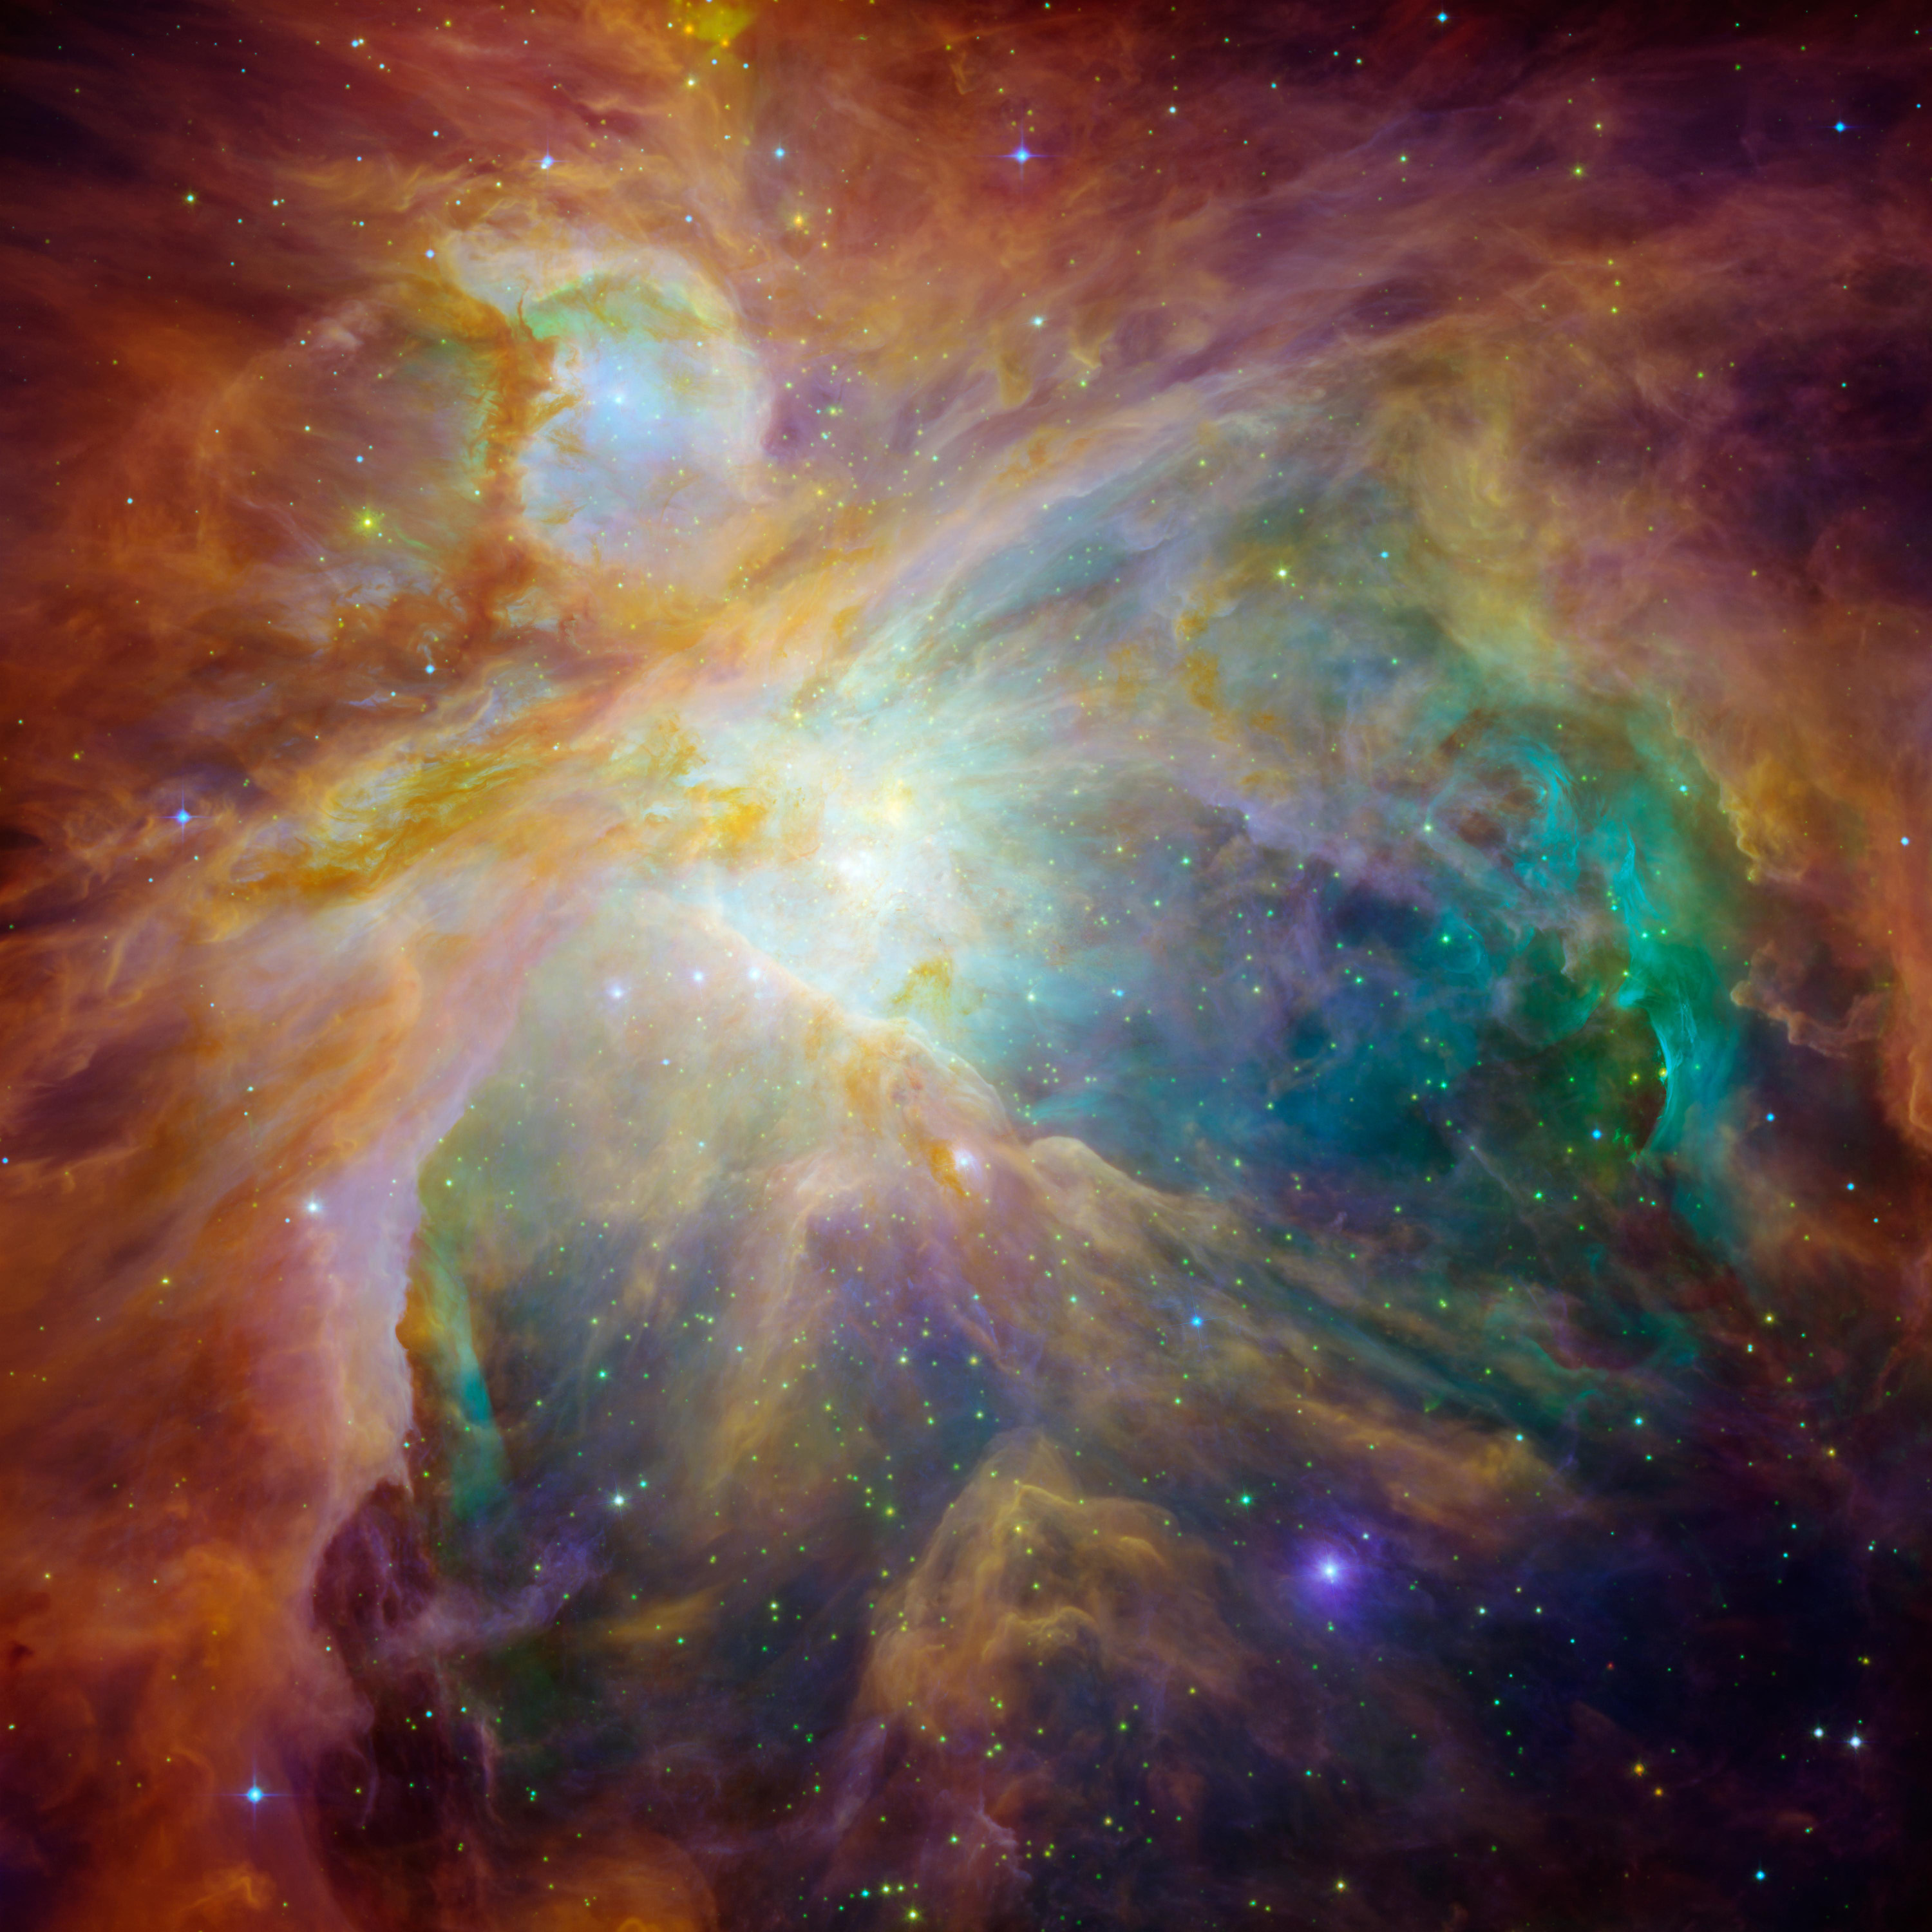
\includegraphics[width=\textwidth]{Figures/orion_nebula}
 \captionsetup{justification=justified,singlelinecheck=false,width=\linewidth}
 \decoRule
 \caption[The Orion Nebula]{The Orion Nebula: a false--color, composite image from NASA's Spitzer Space Telescope (SST) and Hubble Space Telescopes (HST).
			    The SST used its Infrared Array Camera (IRAC), while HST's Advanced Camera for Surveys (ACS) probed in the visible spectrum.
			    Amongst several others, the common H$\alpha$, SII and OIII filters were used to map the observations to rgb colors.\\
			    \textit{Image credit: NASA/JPL--Caltech/STScI}}
 \label{fig:Orion_nebula}
\end{figure}

% Description of the picture ----------------------------------------------------------------------------------------
The right side of the picture shows green and blue regions of heated, ionized gas intensely emitting ultraviolet radiation, evidence for sulfur and hydrogen.
In the left part there are darker clouds in yellow, orange and red color from infrared radiation, showing fewer stars due to the high column density of dust blocking all light below visible wavelengths.
The center shows a very massive, newly formed star cluster, identifiable as a bright yellow smudge, emitting radiation which erodes the region around it, while its stellar winds blow the gas even further away.
This extraordinarily massive cluster is even suspected to hold a black hole, roughly 200 times more massive than our Sun; see \citet{Orion_BH}.
\\[6pt]
%
% ISM ----------------------------------------------------------------------------------------
Molecular clouds are found in the interstellar medium (hereafter ISM), the material between star systems in galaxies.
The ISM is still quite mysterious and there is a considerable number of unsolved problems involving it, yet the physics of the ISM has been subject to research for a long time; see \citet{Draine, Unsolved_Problems}.
It is primarily composed of hydrogen, in atomic, ionized, and molecular form, usually denoted by HI, HII, and H$_{2}$, which leads to a separation into roughly three phases governed by the very different cooling mechanisms which are dominant for each kind.
Although the three--phase theory of the ISM was published over 35 years ago by \citet{ISM_3Phases}, it is still the prevailing model and hasn't been changed drastically since.
Each phase is thought to be in thermal pressure equilibrium, where heating and cooling rates are balanced.
Their equilibrium temperatures are around $10^{6}$ K, $10^{4}$ K, and $10$ K respectively, and their typical densities are $10^{-1}$ H/cc, $1$ H/cc, and $10^{3}$ H/cc.
\\[6pt]
%
% Numbers for MC ----------------------------------------------------------------------------------------
In the broad morphology of molecular clouds, some properties, like total mass, can vary widely and over several orders of magnitude.
Giant molecular clouds can have masses in the range of $10^{4}$--$10^{6}$~M$_{\odot}$ and stretch up to 200 pc in diameter; see \citet{GMC_Masses} and \citet{MC_Masses}.
The main constituent part of the clouds, as their name leads to presume, is molecular hydrogen H$_{2}$.
Typical temperatures in these clouds are around 10 K.
This low--temperature, high--density phase of the ISM is necessary in order to form dense enough regions to offset the balance between gravity and thermal pressure, thereby initiating gravitational collapse to form stars.
Higher temperatures would result in a thermal expansion and consequently in a reduction of the gas density.

% Observation ----------------------------------------------------------------------------------------
Even though the Orion Nebula can partially be seen on clear winter nights due to emission from ionization, most parts of molecular clouds are usually invisible to the naked eye.
The medium is much too cold to radiate in the visible spectrum.
Thus, in the exploration of molecular clouds radio and infrared astronomy is indispensable.
With measurements of radio emission from tracer molecules, such as CO, the structure of the gas clouds can be probed; see \citet{CO_tracing, Lada, Cham_cores_ALMA, Orion_cores}.

% Dust ----------------------------------------------------------------------------------------
Apart from gas, molecular clouds are also laced with dust, small solid grains which are able to absorb radiation below wavelengths of 1 $\mu$m quite efficiently.
The case of extremely high dust column densities blocking all the light from background stars defines another type of molecular cloud, the dark clouds.
Radiation from already formed, highly luminous star clusters in these clouds can excite the dust particles and raise their temperature to almost 100 K.
At the same time, these particles cool and prevent further climbing of their temperature by radiating in the infrared spectrum, which presents another possible method of observation.
\\[6pt]
%
% Turbulence ----------------------------------------------------------------------------------------
Molecular clouds are always highly turbulent, which is probably the main aspect of their beauty, but makes the life of a scientist so much harder; see \citet{Turbulence, KolmogorovC,KolmogorovB,KolmogorovA}.
Completely describing turbulence is a fairly difficult affair, so difficult in fact that it is still one of the unsolved problems in physics.
The origin of turbulence in the ISM is also still an open question.
Nevertheless, it is widely agreed upon that turbulence is a key factor in star formation; see \citet{Turbulence_key}.
Through turbulence energy is cascaded down the scale ladder, which makes star formation a multi--scale process.
How turbulent a cloud is, thus determines the dynamical scale on which the regulatory physics of star formation lie.
As long as turbulence is supersonic, which is observationally confirmed (\citealt{Turbulence_supersonic}), it represents the main contribution of opposing forces in the equilibrium with gravity.
However as turbulence dissipates on smaller scales due to shocks and viscosity, the cloud begins to fragment into clumps: compressed, denser regions, where the turbulent pressure is not strong enough and gravity takes hold.
This fragmentation process can happen repeatedly on different scale levels until gravitationally bound, homogeneous clumps remain.
These smallest clumps are called dense cores~\footnote{in some literatures also called molecular or in early stages starless cores} and ultimately collapse to protostars; usually they result in a whole set of protostars, called star cluster, but rarely in single stars.
\\[6pt]
%
% Importance of radiation ----------------------------------------------------------------------------------------
Once the star clusters have formed the demise of the molecular cloud is imminent.
One might be tempted to think that after the protostars have formed, they start to accrete the remaining gas in the cloud until all the material is consumed and only fully grown stars are left.
Observations and some theoretical considerations tell us another story: star formation is a very inefficient process in the sense that only a small fraction of the total cloud's mass is channeled into collapsing protostars, while most of it is blown outwards to repopulate the diffuse ISM; see \citet{SF_regulation, Padoan_PP}.
An enormous release of kinetic energy within a very short time span, such as a supernova explosion, could be responsible for the disruption of molecular clouds.
Observational estimates for the lifetime of molecular clouds however, are usually much shorter than the time, when the first supernova explosions occur; see \citet{MC_Masses, MC_supernovas}.
Currently the favored scenario which is thought to be responsible for the disruption of molecular clouds, is the ionizing radiation feedback from massive star clusters; see \citet{MC_disruption, Ionizing_disruption}.

\begin{figure}[ht]
 \centering
 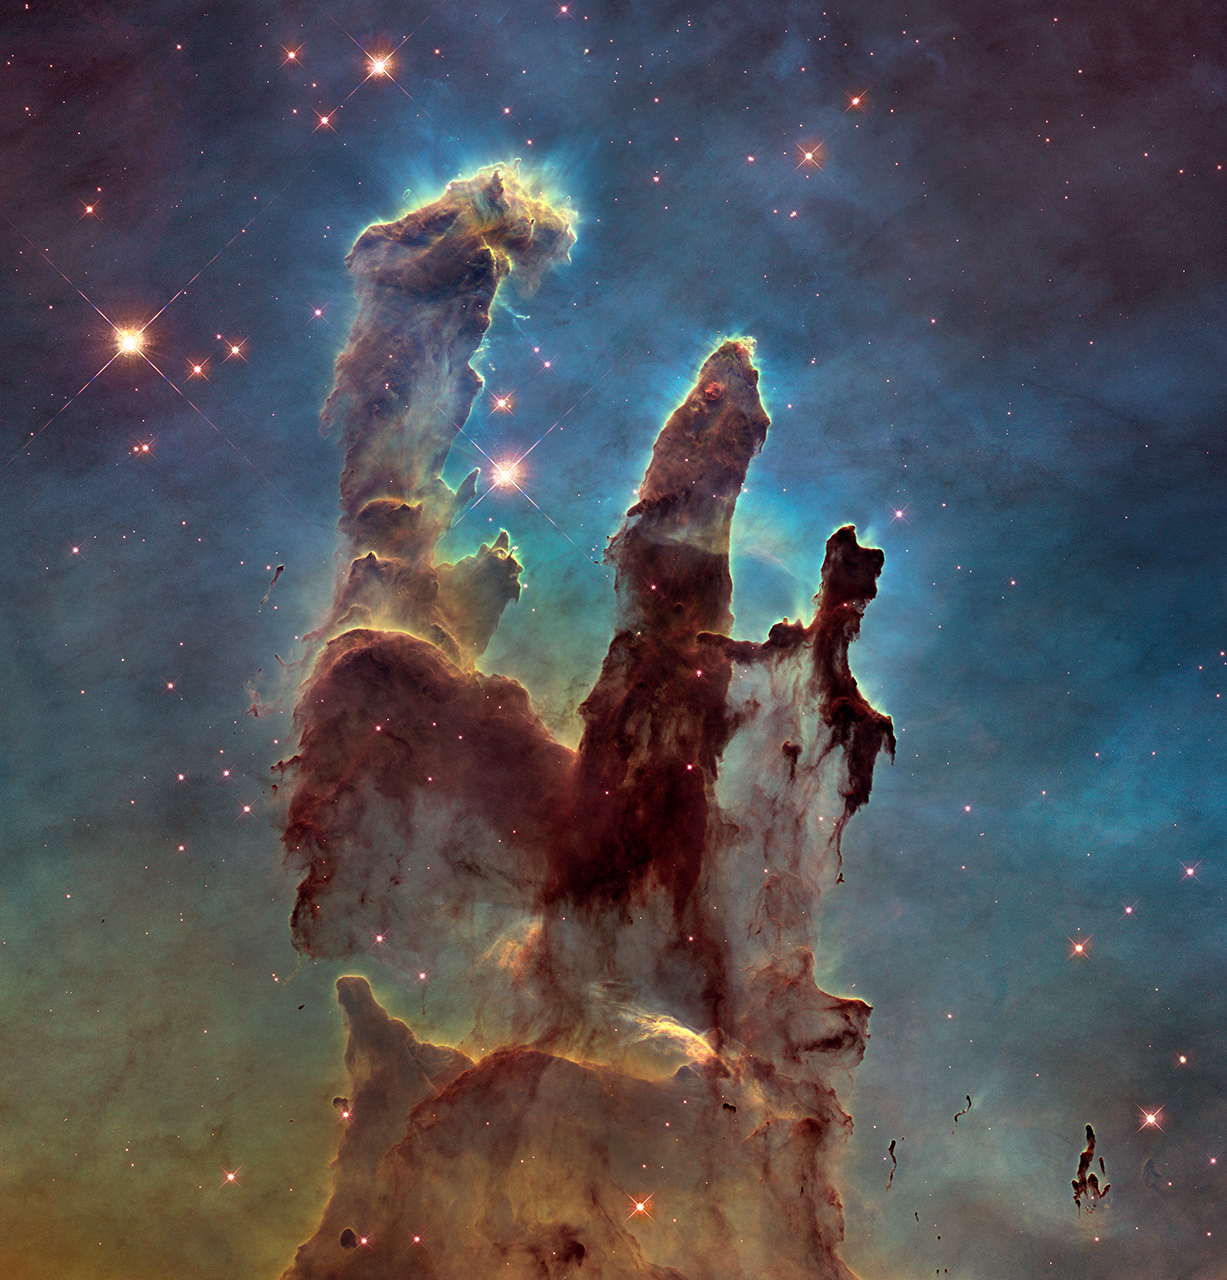
\includegraphics[width=\textwidth]{Figures/pillars_of_creation}
 \captionsetup{justification=justified,singlelinecheck=false,width=\linewidth}
 \decoRule
 \caption[Pillars of Creation]{A high-definition shot of NASA's iconic scenery, the 'Pillars of Creation', found in the Eagle nebula (M16).
          The name epitomizes the speculation that our own sun formed under a very similar nascent environment.
          All physical key processes of star formation are collected in a single picture:
          The pillar--like structure shows the turbulent nature of molecular clouds, while the gleaming tips of the towers show evidence of erosion by the hidden star cluster's radiation. \\
          \textit{Image credit: NASA, ESA/Hubble and the Hubble Heritage Team}
 }
 \label{fig:Pillars_of_creation}
\end{figure}

The influence and importance of radiative feedback is clearly shown in \figfigref{fig:Orion_nebula}{fig:Pillars_of_creation} both.
In \figref{fig:Orion_nebula} the region around the star cluster was already evacuated by its ionizing radiation, whereas in \figref{fig:Pillars_of_creation} the radiation just begun to erode the gas at the top of the pillars.

A standing goal of many computational astrophysicists is to reproduce the formation and evolution of whole galaxies and similar astronomical objects.
Over the years, a great deal of insight has been gained from hydrodynamical simulations, but there are still many open problems and a complete, physical simulation has yet to be run.
However these simulations also made it clear that radiation feedback has to be included and accurately modeled to make it one step further towards a realistic simulation.

% ----------------------------------------------------------------------------------------
\section{More and more questions}

After this short introductory overview on the birth places of stars, we will go into some important aspects of the very complex topic of star formation in more detail in the next few chapters.
To this date, the overall theory of the process of star formation is roughly outlined and in the star formation community to most parts accepted, the details are somewhat vague and debatable at times.
Some aspects have already been tested by numerical simulations --- a strong tool available to theoretical astrophysicists, when dealing with complex multi--physical scenarios ---, others have only now become possible to explore thanks to increasing computing power, and highly scalable and efficient astrophysical hydrodynamics codes.
\\[6pt]
%
% Personal learning process and structure ----------------------------------------------------------------------------------------
This thesis will be a recount of all the things I learned in the past year while working in computational astrophysics on the topic of star formation.
Thus, the following discussions will first cover the basics and impart analytical tools for processes involving hydrodynamical and radiative effects in astrophysics in general.
Due to a very limited starting knowledge in astrophysics when I began in this field of research, I had to ask very basic and at first glance maybe simple, but nonetheless important questions:
\\[-9pt]
\begin{itemize}
  \item Where and under what conditions do stars form? \\[3pt]
        Some answers to this question were outlined in this chapter; see \secref{sec:MolecularClouds}.
        Knowing where stars form, gives insights into the circumstances leading to star formation, which in turn determines the predominant physics involved.
        Once the driving forces are uncovered, the construction of physical models can commence, and raises subsequent question.\\[-9pt]

  \item How does a fluid, particularly molecular gas, move in a self--gravitational potential? \\[3pt]
        In the next \chapref{Chapter2}, \secref{sec:HydrodynamicEquations}, we will see idealized mathematical descriptions of the kinematics of fluids.
        These descriptions can be solved for equilibrium solutions, which give hints to possible configurations favorable for star formation and their instabilities; see \secref{subsec:Hydrostatic_equilibrium}. \\[-9pt]

  \item How does molecular gas collapse and fragment? \\[3pt]
        Behind this question lies importance for physics as well as for computational science.
        Fragmentation, or the lack thereof, can be the result of a multitude of physical processes.
        Investigating all of them is beyond the scope of this thesis.
        Thus, this thesis lays the focus on a single specific effect, which is also part of the next question.
        Of special relevance for fragmentation are mass, length and time scales and conditions for gravitational stability of gas.
        These are also of particular importance for the resolution requirements of (sub--)grid models in computer simulations.
        \secref{subsec:Instabilities} will explain the relevant physics of gravitational collapse and gas fragmentation.
        The description of some of the grid models and their specific requirements are discussed in \secref{sec:AMR}. \\[-9pt]

  \item How does an initially rotating sphere evolve into a star forming core? \\[3pt]
        This question addresses the issue of initial conditions and simplification of given problems.
        The choice of initial conditions depends on the part of the problem one wants to focus on.
        When setting up a simulation for instance, there are important aspects one has to consider in order to realistically reproduce the problem or process.
        What cases are even possible to simulate? Where can simplifications be made without the loss of physics in focus?
        \secref{subsec:Larson_cores}, explains the simplified model which still considers the basic physics involved in star formation.
        \secref{subsec:Initial_conditions}, describes how the initial conditions for these models were numerically implemented. \\[-9pt]

  \item How does radiation and other physical modes influence molecular gas? \\[3pt]
        The second part of the next chapter, \secref{sec:RadiativeTransfer}, introduces the basic theory how radiation interacts with matter.
        Knowing in detail how radiation affects the gas (see \secref{subsec:Coupling_to_HD}) during a certain phase in prestellar collapse could explain some discrepancies between simulations and observations of young star clusters. \\[-6pt]
\end{itemize}

These questions represent my thinking and learning process and should give a common thread through star formation theory.
This thesis consists of part theoretical physics which is structured through the questions above, and part computational science which is discussed in \chapref{Chapter3}.
Computational astrophysicists have already realized that the theory of star formation and radiation hydrodynamics are intertwined, but including radiation in hydrodynamics simulations requires much more computational resources, which is why one often relied on computationally cheaper, but inexact sub--grid models.
To date simulations including both are considered state--of--the--art.
Methods working towards this objective are discussed in \secref{sec:Godunov}, (\ref{sec:MUSCL}), (\ref{sec:Source_terms}) and (\ref{sec:AMR}).

In \chapref{Chapter2} and (\ref{Chapter3}) I gather and present the necessary common knowledge in order to be able to investigate star formation with computer simulations.
These simulations and their results are presented and discussed in \chapref{Chapter4}.
%TODO
The main goal of this thesis was to test the numerical model for radiation hydrodynamics (see \chapref{Chapter4}), specifically the infrared radiation treatment for star formation, which was already implemented in the adaptive mesh refinement code RAMSES, mentioned in \secref{sec:RAMSES}.
The final result of this test will be the simulation of an entire molecular cloud; see \secref{sec:MC}.

% !TEX root = ../main.tex
% Chapter 2 - Theory
\chapter{Radiation Hydrodynamics} % Main chapter title
\label{Chapter2} % For referencing the chapter elsewhere, use \ref{Chapter2}

% Introduction ----------------------------------------------------------------------------------------
The subject discussed in this chapter extends over a large number of disciplines in physics, as its spatial scales of importance can range from microns in high--density plasmas to light years in astrophysical shocks.
Given the right conditions, e.g., in sufficiently hot or dense matter, radiation can carry a large fraction of momentum and energy density in hydrodynamic flows.
In these situations the interaction between radiation and matter becomes non--negligible and the theory describing these effects is referred to as \textit{radiation hydrodynamics}.
% \\[6pt]

Nowadays, many problems, especially in astrophysics, are limited by our understanding of, and ability to model, radiation hydrodynamic effects.
One of the major difficulties is the presence of multiple time scales, which, in a numerical point of view, leads to build explicit--implicit schemes in time.
Since it cuts across a wide range of topics in physics, a technical difficulty consists in finding an informative, and self--contained discussion of the subject, although there are some great works out there; see \citet{Mihalas}, \citet{Rybicki_Lightman}, \citet{Shu_1} and \citet{Castor}.
\\[6pt]
%
Thus, I will divide the following discussion and the rest of this chapter into two parts.
The first part will give a general introduction to non--radiating fluids, and the second part will describe the physics of radiation and its interaction with matter.
\\[6pt]
%
This chapter provides an introduction to the theoretical background needed to describe and understand astrophysical fluids and their dynamics in star formation.


% ----------------------------------------------------------------------------------------
\section{Hydrodynamics equations}
\label{sec:HydrodynamicEquations}
Fluid as in its original meaning, derived from the Latin verb \textit{flu\u{e}re} --- to flow, describes a general form of matter as well as the nature of the object itself.
In fluids the matter is free to flow, meaning that internal stresses, contrary to solids, are primarily isotropic and depend on the local mass and energy density.

% Euler vs. Lagrange ----------------------------------------------------------------------------------------
The way how a flow of a fluid will change the state of matter is determined by the mass density parameter, whereas the velocity field is the parameter which determines the motion of the fluid.
When describing the motion of a fluid, we have to decide, how we choose our point of view; generally this can be done in two ways.
Either, we lay a fixed grid over the fluid and describe each grid point by its determining parameters --- usually given by the thermodynamic functions density, pressure and/or internal energy --- as the fluid flows through the grid, or we define parcels of the fluid and follow them, as their determining parameters change over time.
In classical field theory, these descriptions are called Eulerian, resp. Lagrangian, specification of the flow field.

% microscopic description ----------------------------------------------------------------------------------------
Classically, a coarse--graining assumption is also applied to the fluid picture, i.e. the macroscopic fluid is a result and average of microscopic, statistical motions of particles.
This also means that a particle may have a much higher velocity than the average which is the fluid velocity, but the total distance it covers is much smaller than the cell size; in other words, the free mean path of the particle is much smaller than the cell size, which holds if we are in a relatively high density regime.
\\[6pt]
%
In the following, I will provide a more detailed, analytical approach, to what is discussed above, similar to \citet{Mihalas} or \citet{Shu_2}.
For a not so mathematical, and generally simpler introduction which is more focused on the physical applications, I refer to \citet{Castor}.
\\[6pt]
%
% Boltzmann equation ----------------------------------------------------------------------------------------
The classical and easiest way to introduce hydrodynamics is to consider a microscopic description of the fluid particles.
Describing the evolution of an infinitesimally small fluid element through its particle distribution function $f(\textbf{x}, \textbf{v}, t)$ in phase--space, leads to the so--called Vlaslov (no collision integral) or Boltzmann equation

\begin{equation}
  \frac{\partial f}{\partial t} + \dot{\textbf{x}} \frac{\partial f}{\partial \textbf{x}} + \dot{\textbf{v}} \frac{\partial f}{\partial \textbf{v}} = \Big(\frac{\mathrm{D}f}{\mathrm{D}t}\Big)_{\text{coll.}}
\label{eq:BoltzmannEQ}
\end{equation}

where $\big(\frac{\mathrm{D}f}{\mathrm{D}t}\big)_{\text{coll.}}$ denotes the collision integral of the distribution function.

Under molecular chaos assumption (velocities of particles are uncorrelated prior to collision and independent of position) the collision term can be written with one-particle distribution functions

\begin{equation}
  \Big(\frac{\mathrm{D}f}{\mathrm{D}t}\Big)_{\text{coll.}} = \int_{4\pi}\int_{\mathbb{R}^{3}}\int_{\mathbb{R}^{3}} (f'_{1}f'_{2} - f_{1}f_{2})\, \sigma\, v\, \mathrm{d}\Omega\, \mathrm{d}^{3}v_{1}\, \mathrm{d}^{3}v_{2}
\label{eq:collisionInt}
\end{equation}

where the primed functions denote post--collision one-particle distributions $(f'_{i}=f(v'_{i},t) $ for $ i = 1,2)$, non--primed functions are pre--collision one--particle distribution functions $(f_{i}=f(v_{i},t) $ for $ i = 1,2)$, $\sigma$ is the cross section of the collision, and $v = \lvert v_{1}-v_{2} \rvert = \lvert v'_{1}-v'_{2} \rvert$ the relative velocity.

Assuming detailed balance, i.e., processes or transitions are exactly canceled by its inverse, the material is driven towards local thermodynamic equilibrium (hereafter LTE), where the collisional integral vanishes, since $f_{1}f_{2} = f'_{1}f'_{2}$, and the distribution becomes Maxwellian.
By taking the moments in velocity space of \eqnref{eq:BoltzmannEQ}, and consequently of the particle distribution function, the microscopic nature of the equation is averaged out and the ideal hydrodynamic Euler equations are recovered; see Appendix~\ref{AppendixA} for detailed derivation or \citet{Mihalas}, and \citet{Shu_2}.

% Moments ----------------------------------------------------------------------------------------
The moments of the particle distribution function (multiplied by the mass $m$) are

\begin{align}
  m\cdot \int_{\mathbb{R}^{3}} f(\textbf{x}, \textbf{v}, t)\,\mathrm{d}^{3}v &= \rho(\textbf{x},t) \label{eq:fmoment1} \\
  m\cdot \int_{\mathbb{R}^{3}} \textbf{v} f(\textbf{x}, \textbf{v}, t)\,\mathrm{d}^{3}v &= \rho(\textbf{x},t) \cdot \textbf{u} \label{eq:fmoment2}
\end{align}

where $\rho(\textbf{x},t)$ is the density, and $\textbf{u}$ is the average velocity of the fluid.

% Euler equations ----------------------------------------------------------------------------------------
This leads to the Euler equations in Eulerian form

\begin{align}
  \frac{\partial \rho}{\partial t} &+ \nabla\cdot (\rho\textbf{u})= 0 \label{eq:EulerMass} \\
  \frac{\partial (\rho\textbf{u})}{\partial t} &+ \nabla\cdot (\rho(\textbf{u} \otimes \textbf{u}) + \mathbb{P}) = \rho \textbf{a} \label{eq:EulerMomentum}\\
  \frac{\partial E}{\partial t} &+ \nabla \cdot (E + \mathbb{P}) \textbf{u} = \rho \textbf{a} \textbf{u} \label{eq:EulerEnergy}
\end{align}

where $\mathbb{P} = \int m f w_{i} w_{j}\,d^{3}v$ is the pressure tensor consisting of the outer product of the thermal velocity $\textbf{w} = \textbf{v} - \textbf{u}$, and the fluid's total energy density $E = \frac{1}{2}\,\rho\,\textbf{u}^{2} + \rho\,\epsilon$ as sum of the kinetic energy density and internal energy density $\epsilon$.

With every moment of the Boltzmann equation, a new flux term is introduced.
This procedure could go on infinitely, unless we find a way to cut off the loop, also called closure hierarchy.
In the case for the kinetic Boltzmann equation, one often uses an equation of state (hereafter EOS) to approximate and relate the pressure scalar (and consequently tensor with $\mathbb{P} \approx P\cdot\mathbb{I}$) to the energy or mass density.

At times \eqnref{eq:EulerMass} is also called continuity equation, and describes the conservation of mass in a flow, in fact, all of the equations above describe a conservation law, i.e., for mass, momentum and energy, which is equally important and convenient, when it comes to numerical methods and discretization; see \chapref{Chapter3}.
Similarly, had we considered a non--ideal system, i.e., not at LTE, but with a perturbation in the particle distribution function to first order, we could have recovered the Navier--Stokes equation which has an additional momentum flux term representing viscosity, and in the energy conservation law a heat flux term; see \citet{Enskog_Chapman}.
\\[6pt]
%
% Euler equations in Lagrangian form ----------------------------------------------------------------------------------------
Using the Reynolds transport theorem~\footnote{the three--dimensional generalization of the Leibniz integral rule:
          \begin{equation}
            \frac{\mathrm{d}}{\mathrm{d}t}\int_{\Omega}\textbf{f}\,\mathrm{d}V = \int_{\Omega}\frac{\partial\textbf{f}}{\partial t}\,\mathrm{d}V + \int_{\partial\Omega}(\textbf{v}\cdot\textbf{n})\textbf{f}\,\mathrm{d}A
          \end{equation}
          where $\Omega$ is a time--dependent volume, $\partial\Omega$ its boundary, $\textbf{n}$ the normal vector pointing outwards from the volume surface and $\textbf{f}$ a scalar, vector or tensor.
}
to relate the partial derivatives in space and time to the Lagrangian derivative operator $\frac{\mathrm{D}}{\mathrm{D}t} \equiv \frac{\partial}{\partial t} + \textbf{v} \cdot \nabla$ (sometimes also called material derivative), we can rewrite the Euler equations in their Lagrangian form; see Appendix \ref{AppendixA} for details.
\begin{align}
  \frac{1}{\rho} \frac{\mathrm{D}\rho}{\mathrm{D}t} &= -\nabla \cdot \textbf{u} \label{eq:EulerMassL} \\
  \rho \frac{\mathrm{D}\textbf{u}}{\mathrm{D}t} &= -\nabla \cdot \mathbb{P} + \rho \textbf{a} \label{eq:EulerMomentumL} \\
  \rho \frac{\mathrm{D}\epsilon}{\mathrm{D}t} &= -\mathbb{P}\, \nabla \cdot \textbf{u} \label{eq:EulerEnergyL}
\end{align}
These Eqs.~\eqref{eq:EulerMassL}, \eqref{eq:EulerMomentumL} and \eqref{eq:EulerEnergyL} deal with nonconservative variables and are therefore not as convenient to implement in numerical codes.
Opposed to the Eulerian form, this form of the equations doesn't emphasize the conservation of the specific quantities.
\eqnref{eq:EulerMassL} rather expresses the compression of the fluid, when its motion converges.
The second equation \eqref{eq:EulerMomentumL} essentially summarizes Newton's first law, while the third equation \eqref{eq:EulerEnergyL} describes the first law of thermodynamics, i.e., the mechanical work done by the adiabatic compression of the fluid.
Computationally speaking, when there is a large dynamic range in density, and one needs higher resolution in high density regions, Lagrangian methods tend to be more powerful, whereas when they have to deal with shock relations, they accumulate large errors; see \citet{SPH_shock}.
Nevertheless, there are for astrophysical simulations widely--used Lagrangian codes, e.g., so--called smoothed--particle hydrodynamics codes, exploiting the fact that fluid elements do not require any explicit topology relating them; see \citet{Gadget} for an example of an SPH code.

% Hydrostatic equilibrium ----------------------------------------------------------------------------------------
\subsection{Hydrostatic equilibrium}
\label{subsec:Hydrostatic_equilibrium}

In astrophysics it is always good to have an idea of the given system's equilibrium states.
The system we want to focus upon henceforth naturally is the topic of this thesis, stars.
To be able to analytically derive such an equilibrium solution for stars, i.e. where forces are in exact balance and cancel each other to zero, we have to start from the very simplest case.
To this end, it is fitting to assume a self--gravitating fluid in which motion is absent altogether.
With the additional assumption of spherical symmetry, i.e. $\rho = \rho(r)$, $\mathbb{P} = P(r)$ and $\textbf{a} = \frac{\partial\phi}{\partial r}$, the momentum Euler equation reads

\begin{equation}
  \frac{1}{\rho}\frac{\partial P}{\partial r} = -\frac{\partial\phi}{\partial r}
\label{eq:Hydrostatic_equilibrium}
\end{equation}

where the gravitational potential is given by the Poisson equation, linking it to the mass density

\begin{equation}
  \Delta\phi = 4\pi G\rho
\end{equation}

\eqnref{eq:Hydrostatic_equilibrium} is called the hydrostatic equilibrium equation.
It holds when a fluid is either totally at rest or its flow velocity constant at each point.
Here the gravitational force is balanced by the pressure gradient force.
Pressure gradient forces are an incorporation of Newton's second law and for instance are the reason why our Earth's atmosphere does not collapse under gravity.
Recalling the form of the Laplacian for spherically symmetric systems ($\Delta = r^{-2} \partial_{r}(r^{2}\partial_{r})$), we can combine the hydrostatic equilibrium equation with the Poisson equation and yield the so--called (dimensional) \textit{Lane--Emden} equation

\begin{equation}
  \frac{1}{r^{2}} \frac{\partial}{\partial r} \big( \frac{r^{2}}{\rho} \frac{\partial P}{\partial r} \big) = -4\pi G\rho
\end{equation}

Using an isothermal EOS ($P=c_{s}^{2}\rho$) to connect pressure to the mass density and the sound speed $c_{s}$, we can further derive the isothermal Lane--Emden equation

\begin{equation}
  \frac{1}{r^{2}} \frac{\partial}{\partial r} \big(r^{2} \frac{\mathrm{d}ln\,\rho}{\mathrm{d}r} \big) = \frac{-4\pi G\rho}{c_{s}^{2}}
\end{equation}

This equation has an exact solution for $\rho \to 0$ at $r \to \infty$, which is called the \textit{singular isothermal sphere} profile

\begin{equation}
  \rho(r) = \frac{2c_{s}^{2}}{4\pi Gr^{2}}
\label{eq:SIS}
\end{equation}

This profile has a non--physical singularity at the center of the sphere, i.e. for $r \to \infty$.
To avoid this problem we can impose appropriate boundary conditions and introduce a 'core' radius $r_{0} = \sqrt{\frac{c_{s}^2}{4\pi G\rho_{c}}}$, such that the profile behaves like

\begin{equation}
  \rho(r) = \frac{\rho_{c}}{1+\big(\frac{r}{r_{0}}\big)^{2}}
\end{equation}

where the density within the core radius is $\frac{\rho_{c}}{2}$.
The integrated mass with radius $r \to \infty$ for this profile is nonetheless still infinite, scaling linearly with $r$.
This can be resolved by introducing another radius which truncates the profile.
The resulting non--singular Lane---Emden solution is then called \textit{Bonnor--Ebert} sphere, independently derived by \citet{Bonnor} and \citet{Ebert}.
\\[6pt]
%
Due to the asymptotic behavior for $r \gg r_{0}$ all configurations approach the singular isothermal sphere, especially if they have a high density contrast between center and edge, as it is the case for molecular cores.

Even though the isothermal assumption is the simplest case imaginable, it seems to be well-founded.
In molecular cores the temperature is determined by heating and cooling processes.
On the edge of very dense cores the heating comes from UV radiation of O and B stars and cosmic rays, dominating the cooling from fine--structure, dust, and H$_{2}$ emission.
There, temperatures can reach almost 100 Kelvin, but observations tell us that towards the core center the medium starts to become optically thick such that the heating and cooling rates are balanced out and the temperature is almost constant at 10 Kelvin; see \citet{Goldsmith_cooling, Wolfire_10K}.

% Instabilities ----------------------------------------------------------------------------------------
\subsection{Instabilities and gravitational collapse}
\label{subsec:Instabilities}

To have a feasible analytical description of star formation from core collapse, we need to introduce perturbations to the equilibrium solutions to test its stability.
We therefore start from a self--gravitating equilibrium state with $\rho_{0}$, $v=0$, and an isothermal EOS.
For sake of simplicity we use the one--dimensional Euler equations

\begin{align}
  \frac{\partial\rho}{\partial t} + \rho\frac{\partial u}{\partial x} + u\frac{\partial\rho}{\partial x} &= 0 \\
  \frac{\partial u}{\partial t} + u\frac{\partial u}{\partial x} + \frac{c_{s}^{2}}{\rho}\frac{\partial\rho}{\partial x} &= \frac{\partial\phi}{\partial x}
\end{align}

we only obtain a viable equilibrium state if the background density, a static medium surrounding the state, is ignored.
This has come to be known as the 'Jeans Swindle' and is only valid in Cosmology or rotating systems.

Now small perturbations in density, velocity and potential ($\delta\rho$, $\delta u$, and $\delta\phi$) are introduced to the Euler equations.
By linearizing and combining the equations, we obtain

\begin{equation}
  \frac{\partial^{2}\delta\rho}{\partial t^{2}} - c_{s}^{2}\frac{\partial^{2}\delta\rho}{\partial x^{2}} - 4\pi G\rho_{0}\delta\rho = 0
\end{equation}

Comparing this equation to the general formula of a wave equation, we find the same with an additional term of $-4\pi G\rho_{0}\delta\rho$.
Thence we use a planar wave ansatz $\sim\exp(i(kx-\omega t))$ and recover the dispersion relation

\begin{equation}
  \omega^{2} = c_{s}^{2}k^{2} - 4\pi G\rho_{0}
\end{equation}

Here this additional term has profound ramifications.
Since this argument is negative, it is possible for $\omega^{2}$ to become negative for some $k$.
The planar wave consequently has a real exponent $i\omega$, which means that the oscillatory behavior is replaced by exponential growth.
Therefore any perturbation with k leading to a $\omega^{2}<0$ grows in amplitude, increasing the density more and more.

This happens when the wavenumber $k$, or rather the wavelength $\lambda = 2\pi/k$, exceeds the critical value, known as \textit{Jeans length}

\begin{equation}
  \lambda_{J} = c_{s}\sqrt{\frac{\pi}{G\rho_{0}}}
\end{equation}

Any scale larger than the Jeans length is therefore gravitationally unstable.
\\[6pt]
%
\citet{Shu_paper} did a similar analysis of a core collapse using an expansion wave solution.
The molecular core has initially a singular isothermal sphere profile as in \eqnref{eq:SIS}.
He found that if a perturbation occurs, the sphere starts to collapse from the center outwards, forming a propagating collapse front which moves with the sound speed $c_{s}$.
Since the sphere was in hydrostatic equilibrium at first, it remains static until the collapse front arrives.
This way shell by shell collapses to the center core within a free fall time.

\begin{equation}
  t_{ff} = \frac{\lambda_{J}}{c_{s}} = \sqrt{\frac{\pi}{G\rho_{0}}}
\end{equation}

The core thus grows with a constant mass accretion rate of $\dot{M}_{acc} = \frac{c_{s}^{3}}{G}$.

Typical numbers for molecular cores are $10^{3}\,\text{cm}^{-3}$ for number density, $10\,\text{K}$ for temperature and a sound speed of around $0.2\,\text{km}/\text{s}$.
A Jeans length can also be translated into a critical mass.

\begin{equation*}
  \lambda_{J} \sim 1.0\,\text{pc}\,\,\big(\frac{T}{10\,\text{K}}\big)^{\frac{1}{2}}\,\big(\frac{n}{10^{3}\,\text{cm}^{-3}}\big)^{-\frac{1}{2}} \quad\text{ translates to }\quad M_{J} \sim 26\,\text{M}_{\odot}\,\,\big(\frac{T}{10\,\text{K}}\big)^{\frac{3}{2}}\,\big(\frac{n}{10^{3}\,\text{cm}^{-3}}\big)^{-\frac{1}{2}}
\end{equation*}

As the density in the core rises, its temperature stays roughly the same as long as it remains optically thin to the cooling radiation.
As a result, the Jeans length and critical mass decrease and the collapsing object slowly~\footnote{for human standards, for astronomical standards a free fall time is actually rather quick} fragments into smaller and smaller pieces.

An important conclusion to draw from this is that no minimal limit for star masses has yet been introduced.

% Larson's cores ----------------------------------------------------------------------------------------
\subsection{Larson's cores}
\label{subsec:Larson_cores}

Many different numerical experiments of protostar collapse in molecular cores have shown that the core profile indeed corresponds to the one of a singular isothermal sphere in the early stages of collapse.
\citet{Larson_thesis} investigated in his PhD thesis this topic in great detail, numerically as well as analytically.
In an successive paper \citet{Larson_paper} postulated that due to the self--similar behavior of the Lane--Emden equation, the gravitational collapse proceeds as such.
A dens core forms in the center of the sphere, which has come to be known as the \textit{first Larson core}.

Subsequently the core steadily and isothermally grows in density until the medium becomes optically thick to its cooling radiation, meaning the density reaches the threshold beyond which photons are trapped inside the core and begin to heat up their surroundings.

This threshold is called opacity limit, where the optical depth $\tau \simeq 1$.
Optical depth describes the measure of impenetrability to radiation due to absorption and scattering processes along a path through a medium and is defined as

\begin{equation}
 \mathrm{d}\tau = \kappa_{R}\rho\mathrm{d}x
\end{equation}

where $\rho$ is the gas density, $\mathrm{d}x$ the infinitesimal path length through the medium, and $\kappa_{R}$ the Rosseland opacity average according to \citet{Davisetal}.
The state of the gas, i.e. its temperature, the dust grain size in the gas, and the radiation's wave frequency are all components determining this opacity.

The opacity limit finally introduces a physical length scale for the gravitational collapse of protostellar cores.
It can also be translated to a threshold density for a core which is optically thick to radiation.

\begin{equation}
 \lambda \sim \frac{c_{s}^{2}\kappa_{R}}{G} \sim 4 \text{AU} \qquad \Rightarrow \qquad \rho \sim 10^{-13} \text{g/cc}
\end{equation}

Beyond the threshold the second phase of star formation is initiated, in which the core compression approximately becomes adiabatic.
The core density still rises, but simultaneously the core starts to heat up.
Consequently the internal pressure becomes sufficient enough to decelerate and even stop the collapse at the center, while the outer material is still getting accreted isothermally.
Due to the density contrast of the now hydrostatically equilibrated core and the infalling shells, a shock wave can form.
While the mass linearly grows, gravity causes the core to slowly contract again.

When the core reaches a temperature of around $10^{3}\,\text{K}$ the H$_{2}$ molecules begin to dissociate.
Due to the energy consumption which goes into the molecule dissociation, the collapse turns quasi--isothermal again.
When all the molecules have been disbanded the \textit{second Larson core} forms.
Once again the core pressure becomes sufficient enough to produce a core in hydrostatic equilibrium at around $10^{4}\,\text{K}$.
Similarly to the first time, another shock front arises, when the infalling material crashed onto it.

When all the material has fallen onto the second core and its density and temperature have reached stellar values, the star initiates nuclear fusion.
The evolutionary sequence described by Larson is of course only approximative and does not account for electro--magnetic effects, like ambipolar diffusion, influences from dust, rotation, or other 3D effects.


% ----------------------------------------------------------------------------------------
\section{Radiative transfer}
\label{sec:RadiativeTransfer}
At the turn of the 20th century M. Planck, A. Einstein, L. de Broglie, and many other physicists began to realize that the classical notions 'particle' or 'wave' on their own fail to fully explain quantum--scale objects.
This fact is referred to as particle--wave duality and justifies the idea of describing radiation as a highly relativistic fluid of particles with zero rest mass.
Hence, we can precede in a similar way as in \secref{sec:HydrodynamicEquations} and use a microscopic description of the fluid given by a photon distribution function and infer macroscopic behavior and quantities by taking moments.
Yet, the velocity of a photon is a universal constant $c$, and position and momentum are connected by Heisenberg's uncertainty principle; thus, we cannot use $\textbf{v}$ as a phase--space variable and have to fall back on describing the state of a photon with its frequency $\nu$ and direction it travels $\hat{\textbf{n}}$ instead.

% Intensity ----------------------------------------------------------------------------------------
This leads to the definition of the specific radiation intensity, conveniently expressed in terms of the photon distribution function; see Appendix~\ref{AppendixB} for derivation.
\begin{equation}
  I_{\nu}(\textbf{x}, \hat{\textbf{n}}, t) = \frac{h^{4}\nu^{3}}{c^{2}} f(\textbf{x}, \hat{\textbf{n}}, \nu, t)\,.
\label{eq:spec_intensity}
\end{equation}
In some literatures, like \citet{Rybicki_Lightman}, the specific radiation intensity is rather defined over simple dimensional arguments
\begin{equation}
 \mathrm{d}E = I_{\nu}\,\mathrm{d}S\,\mathrm{d}t\,\mathrm{d}\nu\,\mathrm{d}\Omega
\label{eq:dE_intensity}
\end{equation}


% Moments ----------------------------------------------------------------------------------------
The moments of the specific radiation intensity over solid angle~\footnote{moments of the specific radiation intensity over solid angle and frequency are self--consistently defined as \begin{align*}
															E_{\text{rad}}(\textbf{x}, t) = \int_{\nu} E_{\nu}\,\mathrm{d}\nu \,; \quad\qquad
															\textbf{F}_{\text{rad}}(\textbf{x}, t) = \int_{\nu} \textbf{F}_{\nu}\,\mathrm{d}\nu \,; \quad\qquad
															\mathbb{P}_{\text{rad}}(\textbf{x}, t) = \int_{\nu} \mathbb{P}_{\nu}\,\mathrm{d}\nu
														       \end{align*}
} are
\begin{align}
  cE_{\nu} &= \int_{4\pi} I_{\nu}(\textbf{x}, \hat{\textbf{n}}, t)\,\mathrm{d}\Omega \label{eq:spec_energy} \\
  \textbf{F}_{\nu} &= \int_{4\pi} \hat{\textbf{n}}\,I_{\nu}(\textbf{x}, \hat{\textbf{n}}, t)\,\mathrm{d}\Omega \label{eq:spec_flux} \\
  c\mathbb{P}_{\nu} &= \int_{4\pi} \hat{\textbf{n}}\otimes\hat{\textbf{n}}\,I_{\nu}(\textbf{x}, \hat{\textbf{n}}, t)\,\mathrm{d}\Omega \label{eq:spec_press}
\end{align}

% Radiative transfer equation (homogeneous) ----------------------------------------------------------------------------------------
Given the relation between the specific radiation intensity and the photon distribution function (from \eqnref{eq:spec_intensity}), the Boltzmann equation reads

\begin{equation}
  \frac{\partial I_{\nu}}{\partial t} + c\cdot\hat{\textbf{n}}\cdot\nabla I_{\nu} = 0
\end{equation}

where we disregarded the source term at first.
Commonly this equations is known as the \textit{radiative transfer} equation.
\\[6pt]
%
% Source terms ----------------------------------------------------------------------------------------
To include the source term, we consider $\Delta I_{\nu}$ a change of intensity $I_{\nu}$ along the direction of propagation of a light ray through a medium laced with dust grains.
The radiation along this path over a small distance $\Delta s$ can change through several interaction processes between the photons and the dust grains.

Absorption being an example of such a process, in which radiative energy from photons is used to heat up the dust.
Another 'loss of energy'~\footnote{not meaning a violation of the first law of thermodynamics, but rather an idiomatic expression for the transformation of energy, which is afterwards not contributing to the process in focus.} represents the scattering process, in which a shortly induced excited grain state decays and re--emits a photon.
The photon is usually re--emitted in a deflected angle of the same frequency which can be externally observed with a slight Doppler shift.

We assume all intensity--diminishing effects behave similarly and are proportional to $\Delta s$.
The removal of photons should also vary linearly with the intensity $\Delta I_{\nu}$ itself.
Moreover, it should be proportional to a given total mass density of the gas--dust admixture.
Depending on the incident radiation frequency and the grain size, it is more or less likely that a photon interacts with the dust.
This effect summarized by the opacity parameter $\kappa_{\nu}$.
Thus, the negative contribution amounts to $-\kappa_{\nu}\rho I_{\nu}\Delta s$.

Note that $\kappa_{\nu}$ has units of $cm^2\,g^{-1}$, while $\rho$ has the units of $g\,cm^{-3}$.
The inverse product of both is the photon mean free path $\lambda_{\nu} \equiv \alpha_{\nu}^{-1} \equiv (\kappa_{\nu}\rho)^{-1}$ with units of $cm$.
$\alpha_{\nu}$ is called the absorption coefficient.
The fraction of the traveled path $\Delta s$ to this mean free path is called the optical depth $\Delta\tau_{\nu} \equiv \alpha_{\nu}\Delta s$.
It is a property of the medium in which the radiation travels and is often used to model dust effects without including actual particles in simulations.
If the optical depth is $<1$ the medium is called \textit{optically thin}, whereas if $\tau_{\nu}>1$ it is called \textit{optically thick}.

An increase of radiation along its path is of course also possible.
An example of such a process is thermal emission, in which heated dust grains emit photons to cool down, usually in the infrared spectrum.

We summarize all growth contributions in the definition of the emissivity $j_{\nu}$.
Since $I_{\nu}$ is defined per unit area, we can describe the positive change simply by $j_{\nu}\Delta s$.

% Radiative transfer equation (inhomogeneous) ----------------------------------------------------------------------------------------
This is summed up to

\begin{equation}
  \Delta I_{\nu} = -\kappa_{\nu}\rho I_{\nu}\Delta s + j_{\nu}\Delta s
\label{eq:Source_term_derivation}
\end{equation}

By division of $\Delta s$, we obtain the inhomogeneous radiation transfer equation in the infinitesimal limit

\begin{equation}
  \frac{\mathrm{d}I_{\nu}}{\mathrm{d}s} \equiv \frac{1}{c}\frac{\partial I_{\nu}}{\partial t} + \hat{\textbf{n}}\cdot\nabla I_{\nu} = j_{\nu} - \alpha_{\nu}I_{\nu}
\label{eq:Radiative_transfer}
\end{equation}

where $\frac{\mathrm{d}}{\mathrm{d}s} \equiv \frac{1}{c}\frac{\partial}{\partial t} + \hat{\textbf{n}}\cdot\nabla$ denotes the Lagrangian--like derivative, analogously to the hydrodynamical case.
It actually denotes an absolute derivative of $I_{\nu}$ with respect to path length $s$ along a ray, which is a geodesic in spacetime.
Despite using a specific example to motivate this derivation, this equation holds generally and characterizes the radiation transport through a medium with sink and source effects.
\\[6pt]
%
% Radiative equation moments ----------------------------------------------------------------------------------------
To describe further conservation properties, we again take moments of \eqnref{eq:Radiative_transfer}.
This time, we do not require them to be taken over collisional invariants, but take angular moments $\int_{4\pi}\mathrm{d}\Omega$ and $\int_{4\pi}\hat{\textbf{n}}\,\mathrm{d}\Omega$; again see Appendix~\ref{AppendixB} for derivation.

\begin{align}
  \frac{\partial E_{\nu}}{\partial t} \,+\, \nabla\cdot\textbf{F}_{\nu} &= 4\pi j_{\nu}\,-\, \alpha_{\nu}cE_{\nu} \label{eq:Radiative_energy_moment} \\
  \frac{1}{c^{2}}\frac{\partial\textbf{F}_{\nu}}{\partial t} \,+\, \nabla\cdot\mathbb{P}_{\nu} &= - \frac{\alpha_{\nu}\textbf{F}_{\nu}}{c} \label{eq:Radiative_flux_moment}
\end{align}

These equations connect the radiation specific energy density to the radiation flux and pressure tensor.
The first equation describes the radiation energy conservation, to which both emissivity as well as absorption/scattering processes contribute.
This is not so in the second, momentum conservation equation.
There is no momentum contribution from $j_{\nu}$, since we assumed isotropy of the source emissivity and every term is canceled by its contribution from the opposite direction.

Numerically solving these equations for the whole frequency spectrum would be computationally expensive.
An analytical integration over the whole spectrum is therefore useful.
If an investigation does require a distinction of different kinds of photons, a compromising procedure is to discretize the spectrum into different \textit{groups of photons}.
Those groups follow separate sets of moment equations, which means that the computational effort rises with each photon group.

Integral averages of radiation energy density, flux, and pressure can be simply substituted with their average values $E_{rad}$, $\textbf{F}_{rad}$, and $\mathbb{P}_{rad}$ on the given frequency range individual to each photon group.~\footnote{for simplicity we do not use indices for different photon groups and continue as if we had only a single group}
The opacity frequency--spectrum for real materials is very complicated and must be modeled carefully.
Therefore the absorption coefficients should be weighted differently in averages, depending in which moment equation they appear.

There are several approximations for the mean absorption coefficients, solving different regimes, all with their own advantages and drawbacks.
Two very popular methods are the \textit{Rosseland mean} $\alpha_{R}$ and \textit{Planck mean} $\alpha_{P}$.

\begin{align}
  \frac{1}{\alpha_{R}} &= \frac{\int_{0}^{\infty}\frac{1}{\alpha_{\nu}}\frac{\partial B_{\nu}}{\partial T}\mathrm{d}\nu}{\int_{0}^{\infty}\frac{\partial B_{\nu}}{\partial T}\mathrm{d}\nu} \\
  \alpha_{P} &= \frac{\int_{0}^{\infty}\alpha_{\nu}B_{\nu}\mathrm{d}\nu}{\int_{0}^{\infty}B_{\nu}\mathrm{d}\nu}
\end{align}

where $B_{\nu}$ is the intensity of blackbody radiation, discussed in the next \secref{subsec:LTE}.
Using these means in the frequency--integrated moment equations implies that one assumes the spectral energy distribution of a Planckian, and also that the radiation together with the fluid medium is close to LTE.
This is only possible in optically thick regions, where the mean free path of photons is very short.
They have the advantage that in LTE both can be computed as a function of the local state variables once and for all, as $B_{\nu}$ is a function of temperature, while $\alpha_{\nu}$ depends on density and temperature.

% ----------------------------------------------------------------------------------------
\subsection{Thermal radiation}
\label{subsec:LTE}

Once again analogously to the hydrodynamical equations, the moment hierarchy for the radiative transfer equation can be infinitely continued and has to be closed with some kind of approximation.

To find such a closure relation, we look at a radiation field in LTE.
Since blackbody radiation meets the thermal equilibrium condition by its very definition, we know that radiation intensity is a function depending on only one state variable, the absolute temperature: $I_{\nu} = B_{\nu}(T)$.
This function is determined by the well--known Planck's law.

\begin{equation}
  B_{\nu}(T) = \frac{h\nu^{3}}{c^{2}} \frac{2}{e^{\frac{h\nu}{k_{B}T}} - 1}
\end{equation}

This can also be shown by using the radiation intensity definition from \eqnref{eq:spec_intensity}, and recalling that photons are bosons following the Bose--Einstein statistics $N=2 / (e^{\frac{h\nu}{k_{B}T}} - 1)$, such that the photon distribution function is $f\sim N$ per unit 'Planck volume' $h^{3}$.

If dust or gas interacts with the radiation and is in LTE, by definition their source and sink terms in the radiative transfer equation must cancel.
Then the emitted radiation is also in LTE and we recover Kirchhoff's law.

\begin{equation}
  j_{\nu} = \alpha_{\nu}B_{\nu}
\end{equation}

This is the condition for \textit{thermal radiation}, which is radiation emitted by materials in LTE.
We also recall that integrals over functions like $B_{\nu}$ result in factors proportional to the forth Riemann zeta function.
With \eqnref{eq:spec_energy} and averaging over a certain frequency--range $\Delta\nu$, we recover the Stefan--Boltzmann law

\begin{equation}
  S \equiv \int_{\Delta\nu}\int_{4\pi}j_{\nu}\mathrm{d}\nu\mathrm{d}\Omega = \alpha_{P}caT^{4}
\end{equation}

where $S$ is the angular moment of the frequency--integrated emissivity and $a$ the radiation constant.
The Planck mean $\alpha_{P}$ is only a valid approximation if the photon group covers a sufficiently large frequency range $\Delta\nu$.
Commonly this approximation is applied to a photon group in the infra--red range coupling to dust grains, thereby treating dust as a sub--grid model.

% ----------------------------------------------------------------------------------------
\subsection{Coupling to hydrodynamics}
\label{subsec:Coupling_to_HD}

The radiative transfer equation and its moments does describe the propagation of the light in a fluid medium, but the effect of the radiation on the dynamics of the gas is not yet accounted for.
To that end, we have to couple the radiation equations to the Euler equations.
This is done over the source and sink terms.
For every absorbed, scattered and re--emitted photon, there must be a corresponding amount of momentum and energy missing from the fluid.
The variable susceptibility of the gas to certain frequencies was already treated in the radiative transfer equations with the absorption coefficient $\alpha_{\nu}$.
So all there is left to do is to obey the laws of physics~\footnote{the first law of thermodynamics to be precise}.
Thus the amount of energy from the source and sink terms have to be frequency--integrated and added to the Euler equations with reversed sign.

\begin{equation}
  \Gamma = \int_{0}^{\infty}\alpha_{\nu}cE_{\nu}\mathrm{d}\nu \qquad\text{ and }\qquad \Lambda = \int_{0}^{\infty}\int_{4\pi}j_{\nu}\mathrm{d}\Omega\mathrm{d}\nu
\end{equation}

The frequency--integrated is source term $\Gamma$ is called \textit{heating function}, while the total sink term $\Lambda$ is contrarily called the \textit{cooling function}.
The Euler equation addressing the energy equation therefore becomes

\begin{equation}
  \frac{\partial E}{\partial t} + \nabla \cdot (E + \mathbb{P}) \textbf{u} = \rho \textbf{a} \textbf{u} + \Gamma - \Lambda
\end{equation}

This way the energy components of the gas and the radiation are linked through the source and sink terms in their moment equations.
Concerning the momentum exchange, the same method is applied with the sole difference that the radiative moment flux equation only has a source and no sink term.
This is due to the fact that emitted radiation field is always isotropic.
Consequently the radiation force $\mathcal{F}$ is the momentum gained through absorption.

\begin{equation}
  \mathcal{F} = \int_{0}^{\infty}\frac{\alpha_{\nu}F_{\nu}}{c}\mathrm{d}\nu
\end{equation}

Again to comply with momentum conservation the same term has to be inserted into the momentum Euler equation with opposite sign

\begin{equation}
  \frac{\partial (\rho\textbf{u})}{\partial t} + \nabla\cdot (\rho(\textbf{u} \otimes \textbf{u}) + \mathbb{P}) = \rho \textbf{a} + \mathcal{F}
\end{equation}

It is worth mentioning that even though this coupling of gas and radiation dynamics seems simple, many complicated, atomic processes play a part in it.
The parameter summarizing all these influences is the absorption coefficient $\alpha_{\nu}$.
It depends on the gas density as well as its temperature.
Depending on these gas states different processes dominate, such as (photo--)ionization, recombination, excitation, and fine--structure transitions just to name a few.
\\[6pt]
%
Since radiation propagates with the speed of light, the important treatment of relativity was omitted.
The opacity variables should be in fact computed in the comoving frame, moving with the fluid system.
This means that the dust is modeled having always the same velocity as the gas.
The radiation on the other hand is computed in the laboratory frame.
This causes Doppler effects due to the relative motions between the different coordinate systems.
The work done by the radiation force consequently includes an anisotropic component from the source term.
Thus the presented equations should have relativistic corrections of the order $v/c$.
A detailed discussion of a relativistic description of the microscopic radiative processes in the comoving frame can be found in \citet{Mihalas}.

% ----------------------------------------------------------------------------------------
\subsection{Diffusive limit}
\label{subsec:Diffusion_limit}

The LTE approximations for the moment radiation equations lay the ground work for one of two physically relevant limits, which have to be correctly resolved in numerical simulations.
Applying them on \eqnref{eq:spec_energy} and \eqref{eq:spec_press}, we obtain a simple relation between the radiation pressure and the radiation energy density

\begin{equation}
  \mathbb{P}_{\nu} = \frac{E_{\nu}}{3}\mathbb{I}
\label{eq:LTE_radiation_press}
\end{equation}

This is called \textit{Eddington closure approximation} and holds for any isotropic radiation distribution.

In the radiation's steady state for which all derivatives with respect to time vanish, we recover the \textit{diffusion limit} with the LTE condition $\tau \gg 1$.
Therefore the moment equation for the radiation flux reads

\begin{equation}
  \nabla\cdot\mathbb{P}_{\nu} = -\frac{\alpha_{R}}{c}\textbf{F}_{\nu}
\end{equation}

Plugging in \eqnref{eq:LTE_radiation_press} and integrating over the whole frequency--range yields

\begin{equation}
  \textbf{F} \simeq -\frac{c\lambda_{R}}{3} \nabla E
\end{equation}

Now the diffusive nature in this limit becomes evident.
Replacing the flux term \eqnref{eq:Radiative_energy_moment}, we get a parabolic partial differential equation of the form of a diffusion equation with diffusive coefficient $c\lambda_{R}/3$.
If the source and sink terms can be neglected temporarily, this diffusion equation describes the radiation as a wave spreading according to $x \sim \sqrt{ct\lambda_{R}/3}$.
This can lead to some unphysical propagation speeds, if e.g., $ct/\lambda_{R} < 1$ and the LTE condition is not fulfilled, which can be related to the fact that radiation transport in reality not diffusive and the flux not limited.
It is only valid as long as the photons' mean free path $\lambda_{R}$ is small, such that $\vert\textbf{F}\vert \ll cE$ and the radiation is quickly relaxed into LTE.

The diffusion limit can already be used to construct a closure relation.
By limiting the flux such that it recovers the appropriate limit for given conditions, be it optically thick or optically thin surroundings, a working radiation transfer model can be recovered.
With this closure approximation method arise some advantages, such as its simplicity and possibility to combine with implicit time stepping methods.
A big disadvantage however is the modeling of the flux direction which points in the direction of the radiation energy gradient.
Due to its diffusive behavior the casting of shadows from optically thick regions is impossible, yet an important physical effect in the formation of stars.

The diffusive limit still holds without perfect LTE.
This can be demonstrated by introducing a slight anisotropy to the Planckian and writing the radiative transport equation as an expansion in this small anisotropy parameter.
A following Chapman--Enskog--like analysis would then yield the same result.
Thus, slight deviations from thermal equilibrium are still relatively well described in the diffusive limit.

% ----------------------------------------------------------------------------------------
\subsection{Free--streaming limit}
\label{subsec:Free_streaming_limit}

If the optical depth approaches the opacity limit $\tau \simeq 1$ and $\vert\textbf{F}\vert \simeq cE$, the photon mean free path becomes larger and unless flux limiters are used, the fluid--radiation system might be far from LTE.
We then move into the \textit{free--streaming limit} where the isotropy in angular space is not given and provides flux comparable to the energy density.
The radiation is hence streaming freely in the direction of the flux \textbf{n} and the energy moment equation for the radiation simplifies to

\begin{equation}
  \frac{\partial E_{\nu}}{\partial t} \,+\, c\nabla\cdot\hat{\textbf{n}}E_{\nu} = 4\pi j_{\nu}\,-\, \alpha_{\nu}cE_{\nu}
\end{equation}

which is a simple, linear advection equation apart from the source terms (hence hyperbolic).

% ----------------------------------------------------------------------------------------
\subsection{Preservation of the asymptotic limits}
\label{subsec:Asymptotic_limits}

It is now clear that models of radiative transfer have to provide an accurate treatment of both previously mentioned limits.
\citet{streaming_vs_trapped} proposed a methodology in the context of neutrino transport, which can similarly be applied to photons for our purposes.
In this procedure, two photon groups on the same frequency range are added, splitting the radiation energy into two components $E=E_{t}+E_{s}$.
$E_{t}$ belongs to the \textit{trapped} photon group, whereas $E_{s}$ describes the \textit{streaming} photon group.
The difference between them is that radiation flux for the trapped photons is assumed to be strictly zero, according to the asymptotic limit of $\lambda_{R}\to 0$.
These are then handled as separate groups with the exception that during every computational time step, their partition is updated; see \citet{Joki_IR}.
\\[6pt]
%
Another important approximation which should be able to recover both asymptotic limits is the closure relation.
The previously mentioned closures have been primarily based on the diffusion limit.

However, the so--called M1 approximation for the pressure tensor provides a closure relation, which takes both limits into account.
The frequency--integrated pressure tensor is herein written as $\mathbb{P} = E\mathbb{D}$, where $\mathbb{D}$ is called the \textit{Eddington tensor}.
It assumes either the form of the identity matrix $\mathbb{D}\to\mathrm{I}/3$ in the diffusion limit, or $\mathbb{D}\to\hat{\textbf{n}}\otimes\hat{\textbf{n}}$ in the free--streaming limit.
This motivates the ansatz as linear combination of both.

\begin{equation}
  \mathbb{D} = \frac{1-\chi}{2}\mathbb{I} + \frac{3\chi-1}{2}\hat{\textbf{n}}\otimes\hat{\textbf{n}}
\end{equation}

where the direction of propagation $\hat{\textbf{n}}=\textbf{F}/\vert\textbf{F}\vert$ and the Eddington factor

\begin{equation}
  \chi = \frac{3+4f^{2}}{5+2\sqrt{4-3f^{2}}}
\end{equation}

depends on the reduced flux

\begin{equation}
  f = \frac{\vert\textbf{F}\vert}{cE}
\end{equation}

\citet{M1_approx} first introduced this approximation, based on the idea that the radiation is a Lorentz--boosted Planckian, symmetric around the flux direction.
It reproduces both limiting cases in the asymptotic limit of $f\to0$ for the diffusive limit and the free streaming case for $f\to1$.
Since it leaves the moment flux equation hyperbolic, another advantage lies in the integrability into the Godunov scheme discussed in the next \chapref{Chapter3}.

% !TEX root = ../main.tex
% Chapter 3 - Numerical methods
\chapter{Numerical methods} % Main chapter title
\label{Chapter3} % For referencing the chapter elsewhere, use \ref{Chapter3}

%----------------------------------------------------------------------------------------
The equations presented in \chapref{Chapter2} are very hard to solve due to highly non--linear terms which cause systems to behave chaotic.
Finding analytical solutions is often only possible for a simple enough initial state, in one dimension, or with many simplifying assumptions regarding the interplay of different physical processes.
Accordingly, numerical simulations are indispensable in the investigation of chaotic dynamical systems.
Then again, numerical methods can also introduce spurious errors and even suppress actual chaos.
It is not clear how far these numerical results can be trusted.

It is therefore important to have accurate and dedicated techniques for solving the hydrodynamical and radiative transfer equations in an astrophysical context.
The close resemblance in mathematical form of these equations can be exploited to construct a generic numerical solver.
Basic compatibility of hydrodynamics and radiative dynamics is consequently an inherited feature of such a technique.
Nevertheless, there are still complications in the combination of different physical dynamics, which numerical code have to withstand.

Unfortunately with numerical calculations 'you always get what you pay for', in the sense that accuracy always comes with considerable cost.
The trade--in for accuracy is a quick and usually simpler approximation.
This is why performance and accuracy of numerical codes always have to find a balance which is mostly determined by the computational resources available.

A great many books and articles have been written on numerical methods seeking to maximize both.
In my opinion, the most informative works to which I refer throughout the entire chapter are \citet{Toro, LeVeque, Romain_numerical}.
\\[6pt]
%
Over the years many excellent astrophysical, and cosmological simulation codes have emerged.
Most of them are based on one of two main techniques.~\footnote{hybrid codes have also been attempted recently, e.g. GIZMO from \citet{GIZMO} and AREPO from \citet{AREPO}}

The first category is called \textit{smoothed--particle hydrodynamics} (SPH hereafter) technique introduced by \citet{SPH_gingold_monaghan, SPH_lucy}.
These codes discretize the fluids into finite mass elements, hence the 'particle' in SPH.
The movement of these particles represents the advection with the fluid's flow.
As a consequence their dynamics is described by the Lagrangian formalism of the Euler equations.
SPH codes therefore come with exceptionally high spatial resolution in high--density regions, which makes them so attractive for astrophysical applications.

This leads to the second category which we will focus on in this thesis, the so--called \textit{adaptive mesh refinement} (AMR hereafter) method by \citet{AMR_colella}.
Codes using this approach discretize their computational domain into finite volumes, cells.
Contrary to SPH codes, the fluid dynamics in the AMR method follows the Eulerian description of hydrodynamics, thereby benefiting of the conservative nature of the equations.
To mimic the sensitivity of SPH codes to the density in regions with different spatial resolution, AMR codes allow the definition of a criterion after which they refine their mesh grid, making their cells smaller and smaller until the criterion is fulfilled.
Moreover, AMR codes actually allow the implementation of more than just one of these criteria (and not just limited to density variable), which makes this approach very versatile.
\\[6pt]
%
The simulations presented in this thesis employed the AMR code RAMSES.
It consists of many different modules, and to explain them all would be worth a thesis of its own.

However, this chapter will give some insight in the most basic and relevant~\footnote{to this thesis' topic} methods used in the AMR approach.
The discussion will end with some words on the actual code in the final \secref{sec:RAMSES}.


% Godunov scheme ----------------------------------------------------------------------------------------
\section{Godunov schemes}
\label{sec:Godunov}

Finite volume methods, such as the Godunov scheme, aim to solve (systems of) hyperbolic partial differential equations of the type:

\begin{equation}
  \frac{\partial\textbf{U}}{\partial t} + \nabla \cdot \textbf{F} = \textbf{S}
\label{eq:Conservation_law}
\end{equation}

These equations are usually interpreted as a form of conservation law, where $\textbf{U}$ is a state vector of conserved quantities, and $\textbf{F}$ the conserving flux vector corresponding to these quantities.
In the general case $\textbf{S}$ describes source or sink terms, also depending on the elements of $\textbf{U}$, but for simplicity or idealization, e.g., using states in thermal equilibrium, this term is often neglected.

Hence for demonstrative purposes, we consider in the following examples $\textbf{U}$ to be a single--component, one--dimensional scalar field $\textbf{U} = u(x, t)$, $\textbf{F} = f(u(x, t))$ and $\textbf{S} = s(u(x, t)) = 0$, reducing \eqnref{eq:Conservation_law} to a one--dimensional advection problem.
The generalization to higher dimensions and additional terms is possible, but non-trivial in most cases.

\begin{equation}
  \frac{\partial u}{\partial t} + \nabla \cdot f(u) = 0
\label{eq:1D_Advection}
\end{equation}

In principle, this general equation can be numerically solved by the well--known finite difference method, where the differential operators are replaced by a summation of values from the neighboring grid cell points.
The resulting approximation would be fine as long as it is applied on smooth functions, whereas for shocks and discontinuities, which are everything else than rare in turbulent flows, the errors become too high and the method becomes numerically unstable.

If \eqnref{eq:1D_Advection} is valid on a certain volume $\Omega \subset \mathbb{R}$ the expression can be discretized by dividing it into a finite number of sub--volumes or cells, $\Omega_{i}$.
Mesh grids constructed by this discretization are usually \textit{structured}, that is, of rectangular shape.
We will assume this hereinafter.
In effect, arbitrarily shaped, \textit{unstructured} mesh grids could be imagined, and are not hard to implement with finite volume methods.
However then other problems may come to play, such as high overhead in computer time and memory, because of the much more complicated calculation of fluxes between cells.

If the fluxes at cell boundaries $\partial\Omega_{i}$ are --- amongst other things --- Lipschitz continuous~\footnote{A function $g: \mathbb{R} \to \mathbb{R}$ is Lipschitz continuous, if there exists a constant $L$, s.t. \begin{center}$\vert g(x_{2}) - g(x_{1}) \vert \leq L\cdot\vert x_{2} - x_{1}\vert\qquad$ with $x_{1}, x_{2} \in \mathbb{R}$.\\ \end{center} This ensures that the function (i) is continuous, and (ii) does not change more than up to a certain limit.}, the divergence theorem can be applied on the flux term when integrating over the cell volume.

\begin{equation}
  \frac{\partial}{\partial t}\int_{\Omega_{i}}u\,\mathrm{d}\Omega = - \int_{\partial\Omega_{i}}f(u)\hat{n}\,\mathrm{d}S
\label{eq:Finite_volume}
\end{equation}

This already shows that the temporal evolution of the conserved quantity only depends on the fluxes through the cell boundaries.
Thus, the integral effectively yields (in one dimension) two terms, inflow and outflow.

The key idea in finite volume methods is to approximate the left hand side of \eqnref{eq:Finite_volume} with the average $u_{i}$ of the conserved analytical quantity within the cell $i$, opposed to only using the point difference at the boundaries of the cell in the finite difference method.

\begin{equation}
  u_{i} = \frac{1}{\vert\Omega_{i}\vert}\int_{\Omega_{i}}u\,\mathrm{d}\Omega
\label{eq:lhs}
\end{equation}

where $\vert\Omega_{i}\vert$ is the volume of the cell.

As a result, the solution for $u$ in the flux terms at the cell interfaces (right hand side in \eqnref{eq:Finite_volume}) have to be reconstructed by using values of this piecewise constant function for $u$ from both sides of the cell boundaries; see \figref{fig:Piecewise}.

\begin{equation}
  \int_{\partial\Omega_{i}}f(u)\hat{n}\,\mathrm{d}S = f(u(x_{i+1/2})) - f(u(x_{i-1/2})) = f(u_{i}, u_{i+1}) - f(u_{i}, u_{i-1})
\label{eq:rhs}
\end{equation}

\begin{figure}[ht]
 \centering
 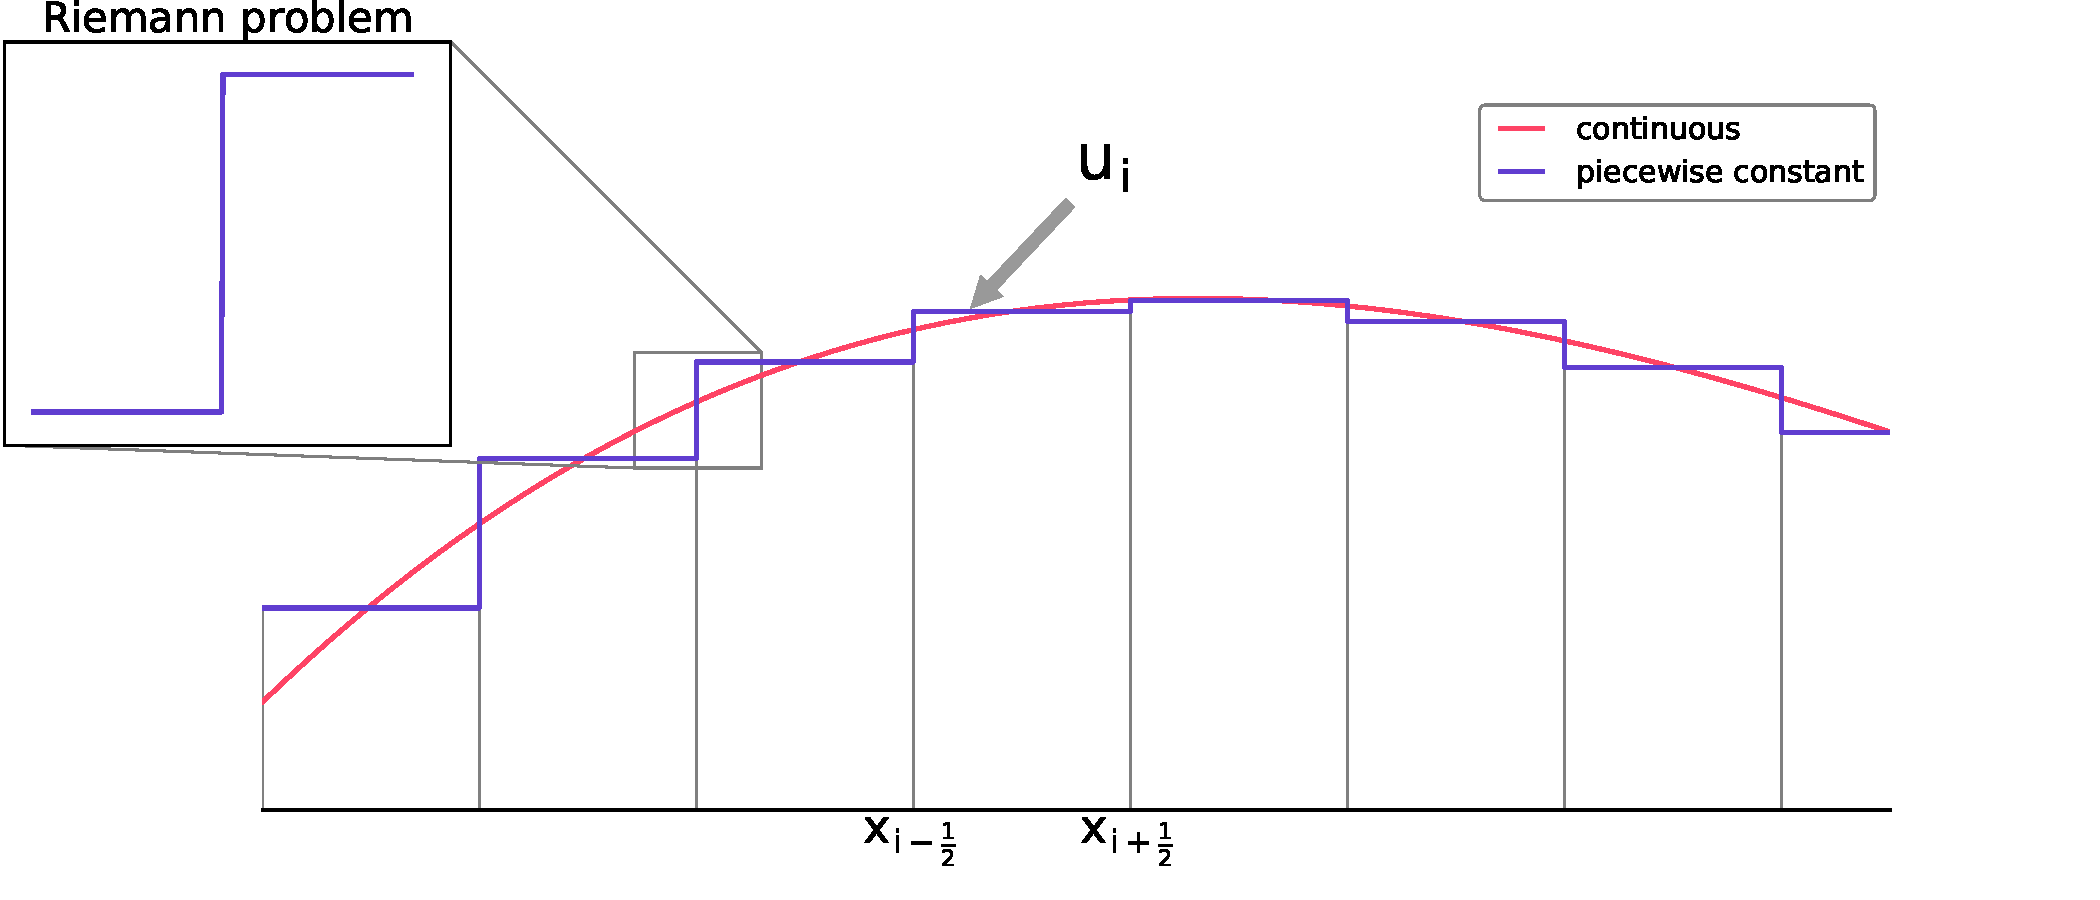
\includegraphics[width=\textwidth]{Figures/piecewise_u}
 \captionsetup{justification=justified,singlelinecheck=false,width=\linewidth}
 \decoRule
 \caption[Piecewise constant function]{A schematic example of the discretization strategy used in finite volume methods.
                                       The continuous function is averaged over the grid cells, resulting in a piecewise constant function, which is stored in memory and used to reconstruct the fluxes in the hyperbolic conservation law.
                                       Each discontinuity at the cell boundaries $x_{i-\frac{1}{2}}, x_{i+\frac{1}{2}}$ etc., describes an individual Riemann problem.}
 \label{fig:Piecewise}
\end{figure}

Inserting Eqs.~\eqref{eq:lhs} and \eqref{eq:rhs} into \eqref{eq:Finite_volume} reads

\begin{equation}
  \frac{\partial u_{i}}{\partial t} =  - \frac{1}{\vert\Omega_{i}\vert} \big(f(u_{i}, u_{i+1}) - f(u_{i}, u_{i-1})\big)
\end{equation}

The complete integral form of this partial differential equation \eqref{eq:1D_Advection} is obtained by another integration in time, propagating the state $u_{i}$ at time $t^{n}$ by a time step $\Delta t = t^{n+1} - t^{n}$

\begin{equation}
  u_{i}(t^{n+1}) - u_{i}(t^{n}) = -\frac{1}{\Delta t} \int_{t^{n}}^{t^{n+1}} \frac{\Delta t}{\vert\Omega_{i}\vert} \big(f(u_{i}, u_{i+1}) - f(u_{i}, u_{i-1})\big)\,\mathrm{d}t
\end{equation}

The above equation is often rewritten in a more algorithmic notation, with upper indices as time step reference and lower indices as cell reference

\begin{equation}
  u_{i}^{n+1} = u_{i}^{n} - \frac{\Delta t}{\Delta x} (f^{n+1/2}_{i+1/2} - f^{n+1/2}_{i-1/2})
\label{eq:Godunov_step}
\end{equation}

where $\vert\Omega_{i}\vert = \Delta x$ is the cell size, $u_{i}$ constant within the cell, and $f^{n+1/2}_{i\pm1/2}$ denotes the flux through the cell boundaries between cell $i$ and $i\pm1$, integrated over a time interval between $t^{n}$ and $t^{n+1}$.
This notation underlines the conservative properties of the equation; in words, the quantity entering through a neighboring cell and the quantity leaving the cell, amount to the change in the quantity itself.
\\[6pt]
%
% Godunov introduction ----------------------------------------------------------------------------------------
It was \citet{Godunov_1959} who first described this kind of finite volume method.
His original scheme uses the analytical solution of the \textit{Riemann problem} which occurs at each cell interface as shown in \figref{fig:Piecewise} (inset), as a building block to calculate the flux terms for \eqnref{eq:Godunov_step}; more in \secref{subsec:Riemann_problem}.
The numerical solution value is updated with the union of all exact Riemann solutions re--averaged over each cell as sketched in \figref{fig:Characteristics}.

In principle, other methods could be used to calculate the numerical flux.
An appropriate flux scheme is best chosen adjusted to the individual problem.
Overall, flux schemes can be classified either as upwind (or Godunov-type) and centered (non-upwind).
The difference between both lies in the explicit use of wave propagation information, which upwind uses, while centered schemes do not.

In the same work Godunov postulated his famous theorem which states that his scheme, and others with constant coefficients preserving monotonicity, can be at most first order accurate.
His work paved the way for many others working on non--linear, high--order schemes, resulting in many variations and extensions of the original Godunov method.


% Riemann problem ----------------------------------------------------------------------------------------
\subsection{Riemann problem}
\label{subsec:Riemann_problem}

A Riemann problem describes an initial value problem for conservation laws like \eqnref{eq:1D_Advection} involving a discontinuity in between two constant regions; see \figref{fig:Piecewise} (inset).
With a discontinuity at $x = 0$ the problem reads

\begin{equation}
  u(x, 0) = \left\{\begin{array}{l l}
            &u_{L} = \text{const.} \hspace{1cm} \text{if} \quad x\leq0\\
            &u_{R} = \text{const.} \hspace{1cm} \text{if} \quad x>0,
            \end{array} \right.
\end{equation}

where $u_{L}$ and $u_{R}$ describe the initial conditions on either side of the discontinuity.
By nature, a variable transform $x' \to cx$ and $t' \to ct$ with $c>0$ preserves the form of the conservation law, such that

\begin{equation}
  u(x, t) = u(\frac{x}{c}, \frac{t}{c}) = u(\frac{x}{t}, 1) \quad \text{for }\,t>0
\end{equation}

This shows that the solution of the Riemann problem is self-similar along constant rays of $\frac{x}{t} = c$, also called characteristics as illustrated in \figref{fig:Characteristics}.

The Godunov flux $f_{i-\frac{1}{2}}$ at $t = 0$  results from an evaluation of $u_{i-\frac{1}{2}}(\frac{x}{t})$ at $\frac{x}{t} = 0$ along the $t$-axis.

\begin{figure}[ht]
 \centering
 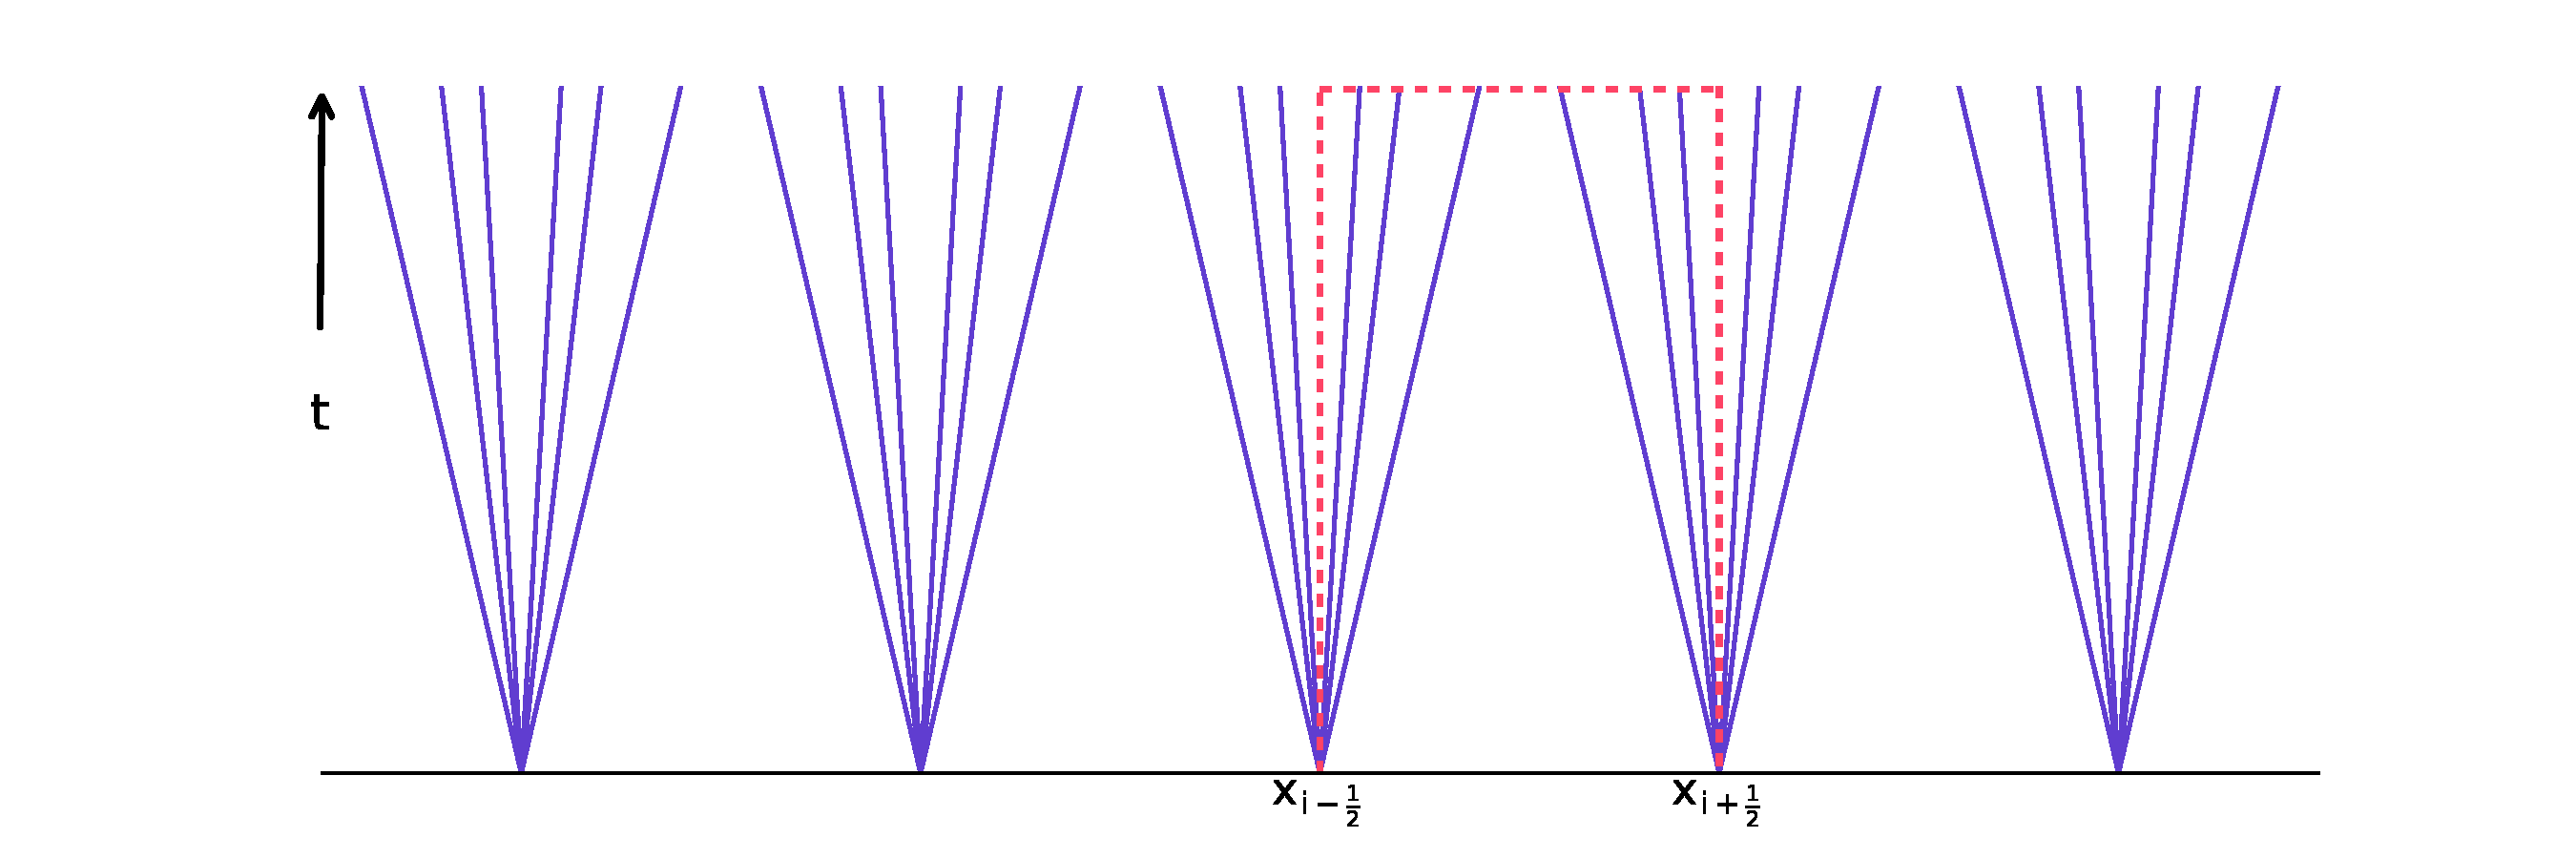
\includegraphics[width=\textwidth]{Figures/characteristics}
 \captionsetup{justification=justified,singlelinecheck=false,width=\linewidth}
 \decoRule
 \caption[Characteristics in Godunov's scheme]{Plot of the characteristics \textit{expansion fans} (blue) of the Riemann problem at each cell interface corresponding to the same discretization as presented in \figref{fig:Piecewise}.
                                               The average of the physical solutions is used to calculate the fluxes in Godunov's scheme (red).}
 \label{fig:Characteristics}
\end{figure}

In its so--called primitive form the conservation law reads

\begin{equation}
  \frac{\partial u}{\partial t} + c\cdot\frac{\mathrm{d}u}{\mathrm{d}x} = 0
\label{eq:Primitive_form}
\end{equation}

with $c=\frac{\partial f}{\partial u}$.
We can reconstruct the Godunov fluxes after an infinitesimal amount of time by using the analytical solution for the Riemann problem as described above.
Therefore we have to consider two cases: (i) $u_{L} > u_{R}$ and (ii) $u_{R} > u_{L}$, yielding the flux

\begin{equation}
  f(u_{L}, u_{R}) = \left\{\begin{array}{l l}
                    &\underset{u_{L}>u>u_{R}}{\text{max}}\big\{f(u)\big\} \hspace{1cm} \text{if} \quad u_{L}>u_{R}\\
                    &\,\underset{u_{L}<u<u_{R}}{\text{min}}\big\{f(u)\big\} \hspace{1cm} \text{if} \quad u_{L}<u_{R}
                    \end{array} \right.
\end{equation}

Since this solution has to be evaluated for every cell interface at every time step, it makes the most computationally expensive task of the whole Godunov method.

Thus, to simplify the process and reduce overhead, Riemann solvers often settle for approximations.
In the following, a few important approximative solvers are mentioned.
\\[6pt]
%
% Roe ----------------------------------------------------------------------------------------
\citet{Roe} for example writes the conservation law, or rather a whole system of conservation laws, in its primitive form as in \eqnref{eq:Primitive_form}, recovering a quasi--linear system with the Jacobian $c=\frac{\partial f}{\partial u}$.
He proceeds by locally replacing $c$ with a piecewise constant matrix for each interval $\tilde{c}(u_{L}, u_{R})$ satisfying the conditions that $\tilde{c}(u_{L}, u_{R})$ (i) is diagonalizable with real eigenvalues, (ii) is consistent with c(u) when $u_{L}, u_{R} \to u$, and (iii) conservative in the flux difference $f(u_{L}) - f(u_{R}) = \tilde{c}(u_{L}, u_{R})\,(u_{L} - u_{R})$.
This way, he achieves linearization of the system.
The flux difference thus depends on the eigenvalues, eigenvectors and characteristics of $\tilde{c}(u_{L}, u_{R})$.
The total flux is then approximated with the so--called upwinding central flux scheme $f_{i-\frac{1}{2}} = \frac{1}{2}(f_{i-1} + f_{i})$, adding these flux difference components.
\\[6pt]
%
% Osher ----------------------------------------------------------------------------------------
Similarly, Osher adds an approximation for $c$ (in \eqnref{eq:Primitive_form}) to the upwinding central flux scheme.
While Roe uses the discontinuities to approximate the Riemann solution, Osher uses $\vert c(u)\vert$, integrated on $u_{R}$ to $u_{L}$ intervals in phase space over simple wave solutions $\int_{u_{R}}^{u_{L}}\vert c(u)\vert\,\mathrm{d}u$; see \citet{Osher_Engquist, Osher_Solomon}.
\\[6pt]
%
% HLL/HLLC ----------------------------------------------------------------------------------------
The approach of \citet{HLL} (HLL hereafter) uses an even simpler approximation.
Whereas Roe and Osher approximate solutions with $N$ intermediate states for a system of $N$ conservation laws, they proposed an approximation of the Riemann solution consisting of two waves separated by three constant states.

\begin{figure}[ht]
 \centering
 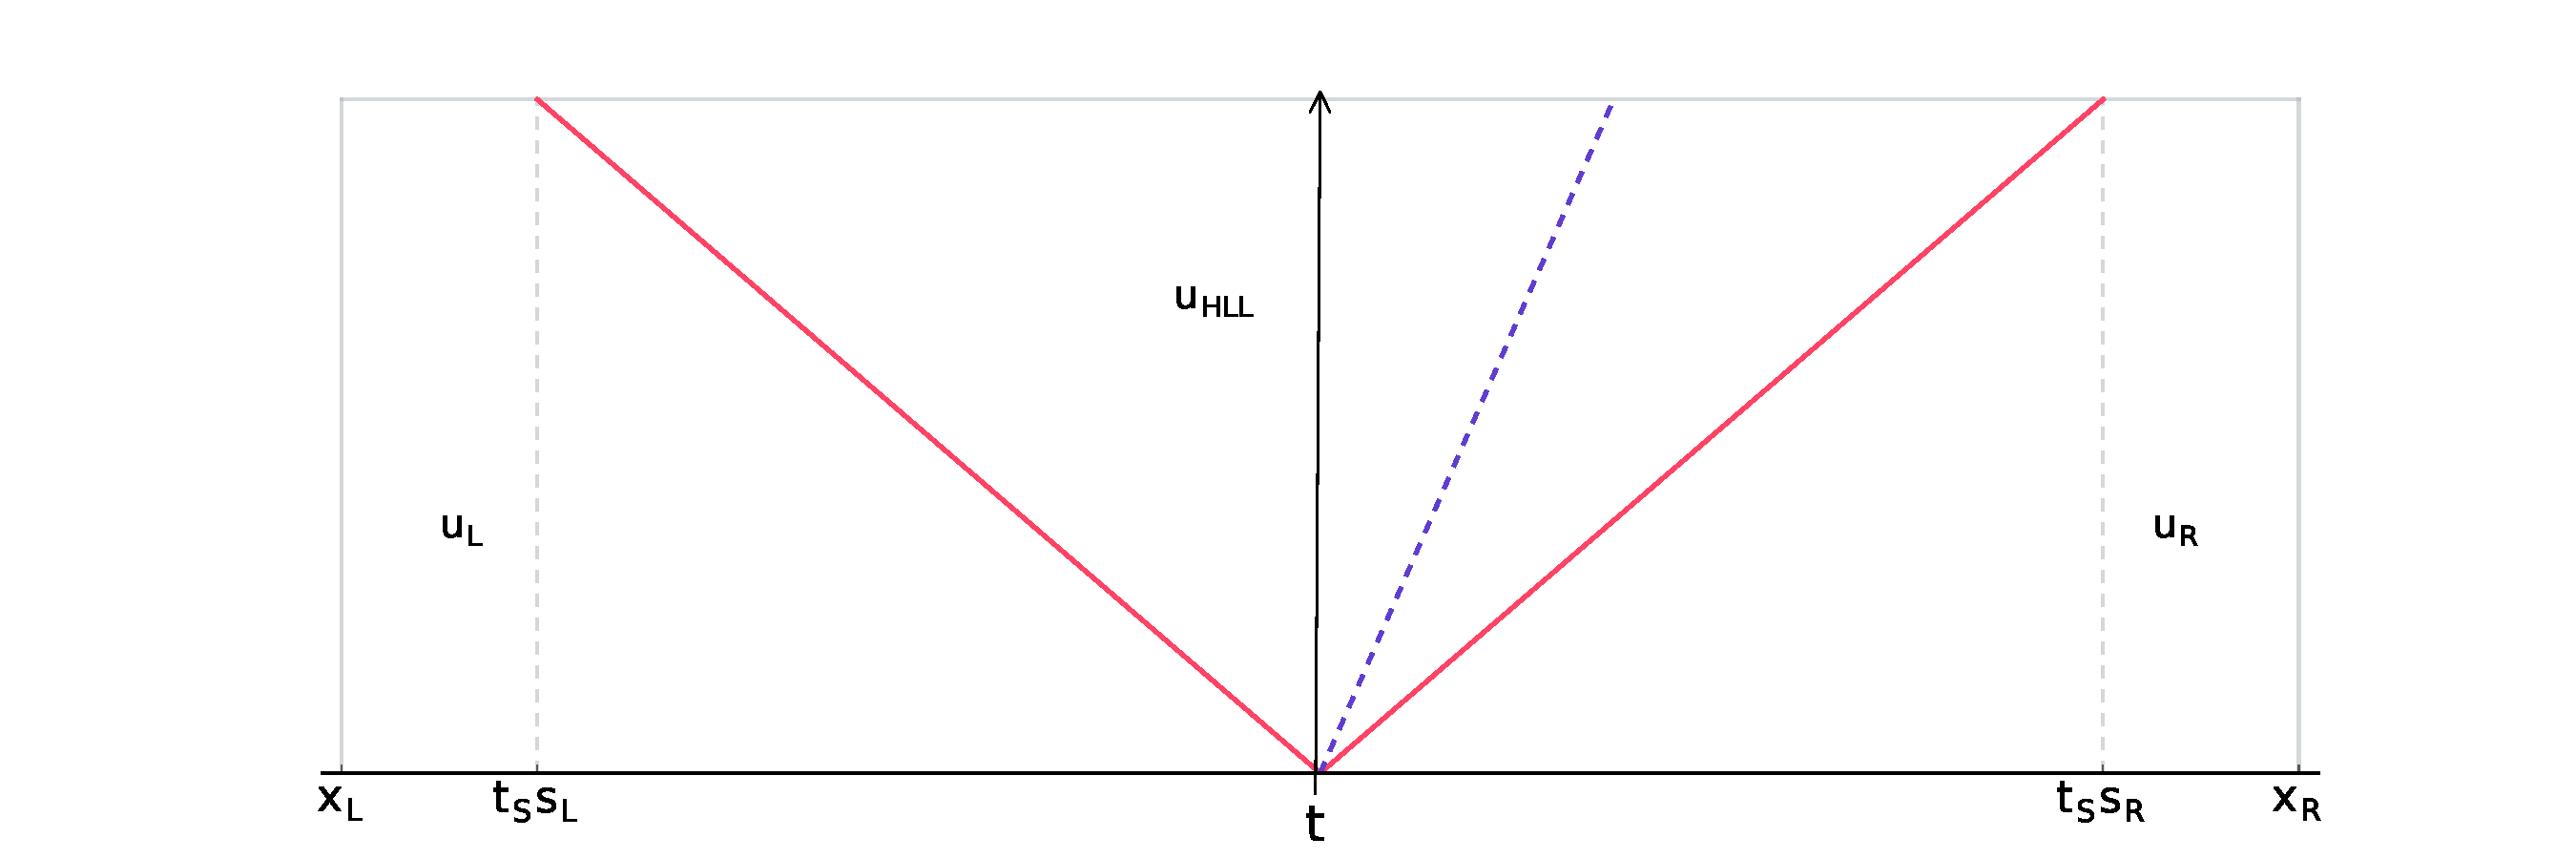
\includegraphics[width=\textwidth]{Figures/hll_regions}
 \captionsetup{justification=justified,singlelinecheck=false,width=\linewidth}
 \decoRule
 \caption[Volume partition in HLL]{The smallest and largest speeds at time $t_{s}$ divide the control volume $[x_{L}, x_{R}]\times[0, t_{s}]$ into three regions.
                                  Here, the limiting characteristics (red) are shown in an $x$--$t$ plot with an example characteristic (blue) in the $u_{HLL}$ state.}
 \label{fig:HLL_regions}
\end{figure}

Choosing a time $t_{s}>0$ the characteristics with speeds $s_{L}$ and $s_{R}$ divide a control volume $[x_{L}, x_{R}]\times[0, t_{s}]$ into three regions according to \figref{fig:HLL_regions} with

\begin{equation}
  x_{L} \leq t_{s}s_{L}\,;\qquad x_{R} \geq t_{s}s_{R}
\end{equation}

where $s_{L}$ and $s_{R}$ are the smallest and largest speeds of a signal resulting from the solution of the Riemann problem.

On this volume the integral form of the conservation law reads

\begin{equation}
  \int_{x_{L}}^{x_{R}} u(x, t_{s})\,\mathrm{d}x = \int_{x_{L}}^{x_{R}} u(x, 0)\,\mathrm{d}x + \int_{0}^{t_{s}} \big(f(u(x_{L}, t)) - f(u(x_{R}, t))\big)\,\mathrm{d}t
\label{eq:Integral_form}
\end{equation}

The integral on the left hand side split into these three regions also yields

\begin{align}
  \int_{x_{L}}^{x_{R}} u(x, t_{s})\,\mathrm{d}x &= \int_{x_{L}}^{t_{s}s_{L}} u(x, t_{s})\,\mathrm{d}x + \int_{t_{s}s_{L}}^{t_{s}s_{R}} u(x, t_{s})\,\mathrm{d}x + \int_{t_{s}s_{R}}^{x_{R}} u(x, t_{s})\,\mathrm{d}x \\
  &= (t_{s}s_{L} - x_{L}) u_{L} + \int_{t_{s}s_{L}}^{t_{s}s_{R}} u(x, t_{s})\,\mathrm{d}x + (x_{R} - t_{s}s_{R}) u_{R}
\label{eq:Integral_split}
\end{align}

Comparing \eqnref{eq:Integral_form} and \eqref{eq:Integral_split}, evaluating the flux integrals with $f_{L,R} = f(u(x_{L,R}, t_{s}))$, and dividing by the width of the wave system of the solution of the Riemann problem between the slowest and the fastest signal $t_{s}(s_{R} - s_{L})$, gives

\begin{equation}
  u_{HLL} \equiv \frac{1}{t_{s}(s_{R} - s_{L})}\int_{t_{s}s_{L}}^{t_{s}s_{R}} u(x, t_{s})\,\mathrm{d}x = \frac{s_{R}u_{R} - s_{L}u_{L} + f_{L} - f_{R}}{s_{R} - s_{L}}
\label{eq:u_HLL}
\end{equation}

The approximate solution to the Riemann problem is therefore defined over this intermediate state $u_{HLL}$.

\begin{equation}
  \tilde{u}(x, t) = \left\{\begin{array}{l l l}
            u_{L} \hspace{1cm} &\text{if} \quad \frac{x}{t}\leq s_{L}\\
            u_{HLL} \hspace{1cm} &\text{if} \quad s_{L}\leq\frac{x}{t}\leq s_{R}\\
            u_{R} \hspace{1cm} &\text{if} \quad \frac{x}{t}\geq s_{R}
            \end{array} \right.
\end{equation}

The corresponding HLL inter--cell flux is then given by the above solution for $\frac{x}{t} \to 0$ same as for the Godunov flux.

\begin{equation}
  f_{HLL} = \left\{\begin{array}{l l l}
            f_{L} \hspace{1cm} &\text{if} \quad 0\leq s_{L}\\
            \frac{s_{R}f_{L} - s_{L}f_{R} + s_{R}s_{L}(u_{R} - u_{L})}{s_{R} - s_{L}} \hspace{1cm} &\text{if} \quad s_{L}\leq 0 \leq s_{R}\\
            f_{R} \hspace{1cm} &\text{if} \quad 0\geq s_{R}
            \end{array} \right.
\end{equation}

It should be noted that the intermediate state $u_{HLL}$ is the mean value of the exact Riemann solution (by definition, see \eqnref{eq:u_HLL}), and if $u_{L}$ and $u_{R}$ are connected by a shock, the correct shock speed is obtained and the solution is exact.

\citet{HLLC} modified the HLL scheme by using an approximate Riemann solution of three waves resulting in two intermediate states, naming it the HLLC scheme.
This way, they achieve the restoration of contact surfaces and shear waves in the Euler equations.

The estimates for the signal wave speeds $s_{L}$ and $s_{R}$ remain to be determined.
They may be evaluated directly over the exact Riemann solution.
Another possibility is to use the averaged eigenvalues of Roe's as estimates.
Or the minimal eigenvalues from the left state and the maximal eigenvalue from the right state could be used to determine $s_{L}$ and $s_{R}$.
The easiest way however is to use the global, maximal signal speed of the simulation on both sides of the discontinuity with corresponding signs (e.g., $s_{L}\equiv-c$ and $s_{R}\equiv c$).
This method is called \textit{global Friedrich--Lax scheme} (GFL hereafter), for which the flux term is finally described by

\begin{equation}
  f_{GFL} = \frac{f_{L}+f_{R}}{2} - c\frac{u_{R}-u_{L}}{2}
\end{equation}


% Numerical diffusion ----------------------------------------------------------------------------------------
\subsection{Numerical diffusion}
\label{subsec:Numerical_diffusion}

The hydrodynamical Euler equations are a set of idealized conservation laws and do thus not describe realistic, physical behavior of a fluid.
They are only valid in the equilibrium state and to obtain a more realistic description, a perturbative treatment leading to higher--order corrections would be needed.

Fortunately, the Godunov scheme (using the GFL method) casts the ideal conservation laws into a modified form.
This is similar to using an infinite Taylor expansion of the conservation law in the finite difference scheme.
Since numerical methods do not work with infinite series~\footnote{unless they converge, which is unlikely}, we have to cut the Taylor expansion at some point.
This introduces a truncation error, often referred to as \textit{numerical diffusion}.
The 'actual' equation solved by the Godunov scheme is a combination of a hyperbolic and a parabolic partial differential equation.

\begin{equation}
  \frac{\partial\textbf{U}}{\partial t} + \nabla\cdot\textbf{F} = \nu_{num}\Delta\textbf{U}
\end{equation}

In GFL this numerical diffusion coefficient $\nu_{num} = \frac{c\Delta x}{2}$ is maximal (for hydrodynamics usually estimated with the sound speed $c_{s}$ as $c = \mathrm{max}\big\{ \vert v_{L}\vert + c_{s}, \vert v_{R}\vert + c_{s} \big\}$).
It is desirable to minimize the truncation error as much as possible, although without any numerical diffusion at all the time integration becomes unstable.


% MUSCL ----------------------------------------------------------------------------------------
\section{MUSCL scheme}
\label{sec:MUSCL}

% Godunov advantages ----------------------------------------------------------------------------------------
The advantage of a Godunov--type scheme is the clear physical picture, it is built on.
Instead of replacing an infinite Taylor series with a truncated one, it conforms a complexly structured physical system to a simple data representation.
This data is exactly evolved for a time step.
The result is then re--simplified similarly as before, preparing it for the next temporal propagation.

However, Godunov himself proved that stable, linear schemes achieve at most first order accuracy.
Hence it can be very diffusive and smearing around discontinuities.
On the other hand, higher order classical schemes which produce sharper discontinuities, but also spurious oscillations around them, possibly attain unphysical values.

From a physical point of view, it is thus immensely appealing to use a Godunov-type scheme's advantages and still carry the accuracy of the data description to higher orders to gain structural resolution.
\\[6pt]
%
% Piecewise linear ----------------------------------------------------------------------------------------
This is achieved by changing the averaging of cell states by moving from a piecewise constant function to another function, say a piecewise linear function as depicted in \figref{fig:Piecewise_linear}.
Such type of method is called MUSCL scheme (Monotonic Upstream--centered Scheme for Conservation Laws), although it was originally the name of P. Woodward's program incorporating B. van Leer's ideas.
There are approaches which extend the idea even further and replace it by a piecewise parabolic function; see \citet{PPM_Colella}.

The new description of the data representation could look something like

\begin{equation}
  u_{i}(x) = \bar{u}_{i} + \frac{\Delta_{i} u}{\Delta x} (x - x_{i})
\end{equation}

where $\bar{u}_{i}$ is the piecewise constant value from the Godunov scheme, $x_{i}$ the center coordinate of the cells, $\Delta x$ the cell size, and $\frac{\Delta_{i} u}{\Delta x}$ the slope, which remains to be determined.

There were several proposals from \citet{MUSCL_1, MUSCL_2} how to express the slope

\begin{itemize}
  \item either the Godunov averaged cell values $\Delta_{i} u = \frac{1}{2}(u_{i+1} - u_{i-1})$
  \item or the difference of the underlying continuous function $\Delta_{i} u = u(x_{i+\frac{1}{2}}, t) - u(x_{i-\frac{1}{2}}, t)$ at the cell interfaces
  \item or using a combination like $\Delta_{i} u = \frac{12}{(\Delta x)^{2}}\int_{x_{i-\frac{1}{2}}}^{x_{i+\frac{1}{2}}} u(x, t) (x - x_{i}) dx$
\end{itemize}

\begin{figure}[ht]
 \centering
 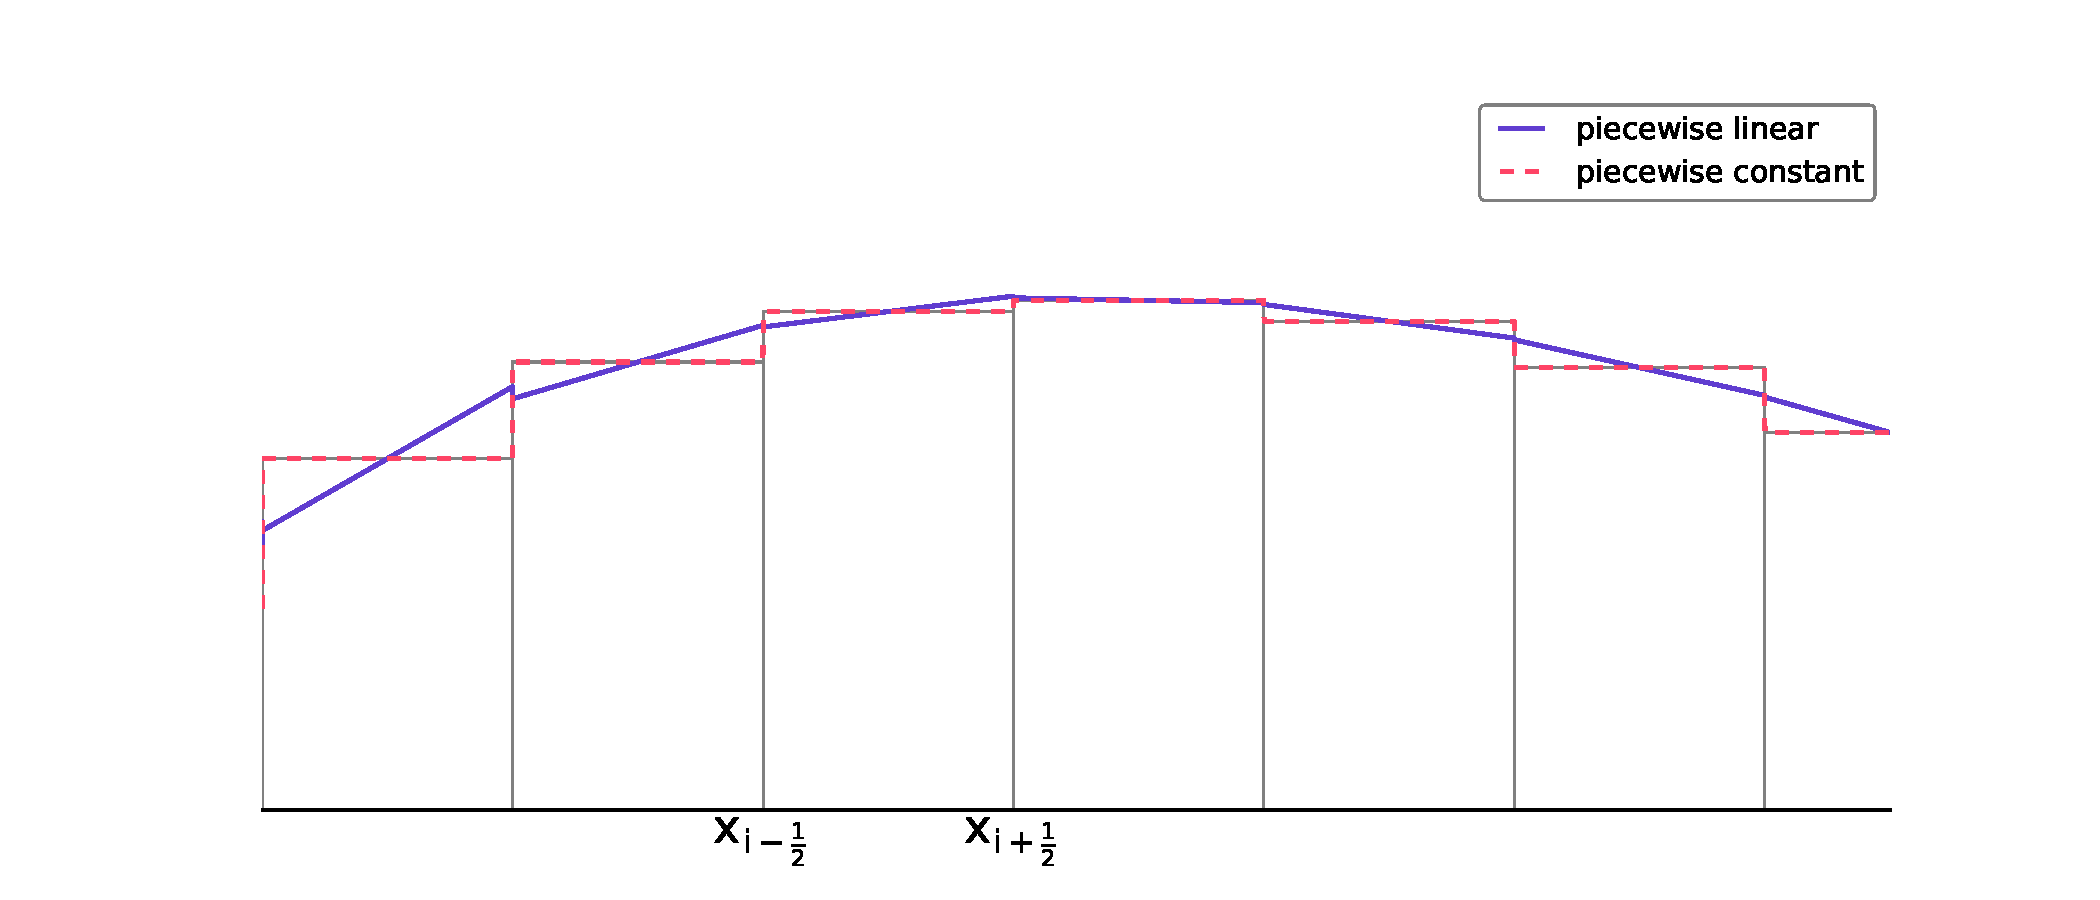
\includegraphics[width=\textwidth]{Figures/pw_linear}
 \captionsetup{justification=justified,singlelinecheck=false,width=\linewidth}
 \decoRule
 \caption[Piecewise linear function]{A schematic example of the extension from first order Godunov scheme to higher orders.
                                     The piecewise constant data representation is replaced by a piecewise linear function, moving up from first order to higher accuracy.}
 \label{fig:Piecewise_linear}
\end{figure}

These lift the accuracy up to second order.
However, there is a catch to changing the data representation, which often renders the method unstable.

% TVD ----------------------------------------------------------------------------------------
To make possible problems more evident, we consider a property of discretization schemes introduced by \citet{Harten_TVD}.
The discretized total variation is

\begin{equation}
  TV(u) = \sum_{i} \vert u_{i} - u_{i-1}\vert
\end{equation}

If the total variation decreases or at least stays the same with time steps, i.e. $TV(u^{n+1}) \leq TV(u^{n})$, the scheme is called \textit{total variation diminishing} (TVD hereafter).
Harten proved that numerical schemes are called \textit{monotonicity preserving} if they are TVD and vice versa.

To outline differences between piecewise constant and piecewise linear schemes, we consider an underlying analytical function with local extrema.
The piecewise constant data representation of the underlying function generally underestimates the absolute value of local extrema provided sufficient spatial resolution.
In the case of a piecewise linear scheme it is possible that the values are overestimated assuming the curvature around the extrema is relatively high.
This causes non--physical oscillations with growing amplitudes around the extrema, rendering the scheme potentially unstable.
Such oscillations increase the total variation, thereby breaking the TVD property.
As follows, total variation evidently makes an excellent monitor of a scheme's oscillatory behavior.
Thus, a monotonicity preserving scheme of higher order is desirable.
\\[6pt]
%
% slope delimiters ----------------------------------------------------------------------------------------
To preserve monotonicity in otherwise monotonicity destroying schemes, but to still profit of higher order strategies, \textit{slope limiters} are introduced.
As the name gives away, they define a limit for the slope of $u$ beyond which the improving scheme is locally reverted back to a piecewise constant scheme, i.e. with a slope equal to zero.

\citet{vanLeer_fluxlimiter} defined his symmetrically monotonized central slope limiters (MonCen hereafter) as

\begin{equation}
  (\Delta_{i} u)_{\text{MonCen}} = \left\{\begin{array}{l l}
                                    \text{sgn}(\Delta_{i} u)\text{min}\big\{ 2\vert\Delta u_{i-\frac{1}{2}}\vert, \vert\Delta_{i} u\vert, 2\vert\Delta u_{i+\frac{1}{2}}\vert \big\} \hspace{1cm} & \text{if} \quad \text{sgn}(\Delta u_{i-\frac{1}{2}}) = \text{sgn}(\Delta u_{i+\frac{1}{2}}) \\
                                    0 \hspace{1cm} &\text{otherwise}
                                   \end{array}\right.
\end{equation}

where $\Delta u_{i\pm\frac{1}{2}} = \pm(u_{i} - u_{i\pm1})$ are the slopes to the left, resp. right side.
These limiters prevent the slope to exceed the range of values of neighboring cell averages
Would the slope take values outside the range between the limits, it instead reverts to the first order description.
This way monotonicity is preserved by excluding the problematic cases.
The limits work for any of the choices for $\Delta_{i} u$ from above.

For the first choice of slope the limiter can be written as

\begin{equation}
  \phi_{VL}(r_{i}) = \frac{r_{i} + \vert r_{i}\vert}{1 + \vert r_{i}\vert}
\end{equation}

where $r_{i} \equiv \frac{u_{i-\frac{1}{2}}}{u_{i+\frac{1}{2}}} = \frac{u_{i} - u_{i-1}}{u_{i+1} - u_{i}}$ is the ratio of slopes on the left and the right.
Unfortunately, in certain situations the MUSCL scheme is still unstable with MonCen limiters.

Another much less aggressively restrictive strategy is the MinMod limiter by Roe; see \citet{Sweby}.

\begin{equation}
  (\Delta_{i} u)_{\text{MinMod}} = \left\{\begin{array}{l l}
                                   \text{min}\big\{ \vert\Delta u_{i-\frac{1}{2}}\vert, \vert\Delta u_{i+\frac{1}{2}}\vert \big\} \hspace{1cm} & \text{if} \quad \text{sgn}(\Delta u_{i-\frac{1}{2}}) = \text{sgn}(\Delta u_{i+\frac{1}{2}}) \\
                                   0 \hspace{1cm} &\text{otherwise}
                                   \end{array}\right.
\end{equation}

If the signs of the slopes on the left and right are the same, the one with the minimal modulus is chosen, otherwise the scheme locally reverts to first order.

With any higher order Godunov--extension scheme, the Riemann problems have to be generalized.
States flanking the discontinuity due to the particular discretization strategy are not constant anymore.
This breaks the self-similarity of the constant Riemann problem, thereby causing the characteristics to bend.
The flux cannot be described by \eqnref{eq:rhs}, which makes exact flux reconstruction harder.
In this case, a predictor step is usually used to approximate the values of the conserved quantities at cell edges at $t+\Delta t/2$.
These predicted values are then used to non--linearly reconstruct the fluxes and update the solution to $t+\Delta t$.
By doing so, a higher--order reconstruction is used for a linear scheme, which does not violate Godunov's theorem.

There are many schemes carrying the idea of extending the Godunov method even further, making modifications in many aspects.


% Source terms  ----------------------------------------------------------------------------------------
\section{Source terms}
\label{sec:Source_terms}

Traditionally source terms refer to inhomogeneous contributions in (hyperbolic) partial differential equations, as in \eqref{eq:Conservation_law}.
So far these terms have been ignored for sake of simplicity.

Sometimes it is appropriate to write the source term as a relaxing deviation from an equilibrium state

\begin{equation}
  \textbf{S}(\textbf{U}) = \frac{\textbf{U}_{eq} - \textbf{U}}{t_{relax}}
\end{equation}

where $\textbf{U}_{eq}$ is the equilibrium state, such that $\textbf{S}(\textbf{U}) \to 0$ for $\textbf{U} \to \textbf{U}_{eq}$, and $t_{relax}$ of the order of a relaxation time scale.
%This can be approximated with the characteristic linear slope of the source term.
%
% \begin{equation}
%   t_{relax} = \big(\mathrm{Tr}(\frac{\partial\textbf{S}}{\partial\textbf{U}})\big)^{-1}
% \end{equation}

With the Godunov solver (especially simple with GFL) we associate another intrinsic time scale, determined by the so--called \textit{Courant factor}

\begin{equation}
  \Delta t = \frac{\Delta x}{c}
\end{equation}

where $c$ is the maximal signal speed in the characteristics associated to a Riemann problem.

Incorporating the source term with the 'homogeneous' Godunov solver is therefore only possible in certain situations.
If the Godunov time scale is smaller than the relaxation time, $t_{relax} > \Delta t$, then the process of the homogeneous part of the conservation law (e.g. the hydrodynamical flow) is much faster compared to the physical process given by the source term.
If on the other hand $t_{relax} < \Delta t$, the source term needs to be carefully coupled to the homogeneous part.
If so, the source term is called \textit{stiff}.
\\[6pt]
%
In the non--stiff regime the most common method to solve hyperbolic partial differential equations with source terms is the \textit{operator--splitting approach}.
Its basic idea is to use fractional steps, splitting the full non--homogeneous conservation law into the homogeneous equation supplemented by the ordinary differential equation

\begin{equation}
  \frac{\mathrm{d}\textbf{U}}{\mathrm{d}t} = \textbf{S}(\textbf{U})
\end{equation}

alternatively solving one then the other equation within a full time step.
First a temporary state is calculated with the previously mentioned Godunov scheme.

\begin{equation}
  \textbf{U}^{n+\frac{1}{2}} = \textbf{U}^{n} - \Delta t \nabla \cdot \textbf{F}(\textbf{U}^{n})
\end{equation}

In an explicit time step the temporary state is used to account for the source term.

\begin{equation}
  \textbf{U}^{n+1} = \textbf{U}^{n+\frac{1}{2}} + \Delta t \textbf{S}(\textbf{U}^{n})
\end{equation}

If the source term tends to stiffness, a much more suited implementation of the source term is an implicit time step, in which the source term depends on the solution of the following time step.

\begin{equation}
  \textbf{U}^{n+1} = \textbf{U}^{n+\frac{1}{2}} + \Delta t \textbf{S}(\textbf{U}^{n+1})
\end{equation}

This obviously complicates the calculation.
Solving for the still unknown solution $\textbf{U}^{n+1}$ then often requires iterative Newton--Raphson root finding algorithms for possibly, highly non-linear terms and fast approximators for the Jacobian which is required for the algorithm.

In the particular case when the source term describes heating and cooling functions, the implicit source--term--related time step is often referred to as \textit{thermochemistry step}.
If the Newton--Raphson algorithm in this case does not converge, one commonly resorts to a subcycling method.
Herein the time step is again split into a number of substeps with the condition that the final result does not increase more than up to a predefined limit.
This limit is usually defined over the factor of $0.1$, accordingly called the \textit{10\% rule}.

\begin{equation}
  \vert \textbf{U}^{n+1}-\textbf{U}^{n}\vert \leq 0.1\times\textbf{U}^{n}
\end{equation}

With these methods the strict conservation of the state variables may not apply anymore.
If this is of special interest, there is almost no choice left, but to directly include the source term in the Godunov scheme in a single implicit time step, thereby leaving the operator--splitting approach.

\begin{equation}
  \textbf{U}^{n+1} = \textbf{U}^{n} - \Delta t \nabla \cdot \textbf{F}(\textbf{U}^{n+1}) + \Delta t \textbf{S}(\textbf{U}^{n+1})
\end{equation}

\citet{LeVeque_source_balancing} proposed an alternative approach to deal with source terms which he called \textit{source--balancing}.
His basic idea was to introduce another discontinuity in the center of each cell through a decomposition of the piecewise constant values into $\textbf{U}_{i}^{-}$ and $\textbf{U}_{i}^{+}$.
If somehow possible, this should be done conservatively such that

\begin{equation}
  \textbf{F}(\textbf{U}_{i}^{+}) - \textbf{F}(\textbf{U}_{i}^{-}) = \Delta x\textbf{S}(\textbf{U}_{i})
\end{equation}

If the decomposition was chosen appropriately, as a consequence the source term in the cell is exactly canceled by the newly introduced Riemann problem.
The source term can therefore be excluded in the Godunov solver, which now simply has doubled workload.
\\[6pt]
%
How to deal with source terms and their stiffness is of course also dependent on the individual problem at hand.
In the following, some important source term versions are briefly discussed.


% Gravitational source terms  ----------------------------------------------------------------------------------------
\subsection{Self--gravity}
\label{subsec:Gravity_source}

The probably most important source term in astrophysics is gravity.
For a very massive group of bodies, gravity dominates over all other forces and is the bonding force, which holds the group together.
Such a group of bodies is then referred to as \textit{self--gravitating}.

Since gravity is a long--range force and practically ubiquitous, it is usually by default already accounted for in the hydrodynamical Euler equations as an external force field; see \eqnref{eq:EulerMomentum} and \eqref{eq:EulerEnergy}.
It is specified by the gravitational potential gradient which in turn is related to the mass density through the Poisson equation.

\begin{equation}
  \textbf{a} = -\nabla\phi \qquad\text{ and }\qquad \Delta\phi = 4\pi G\rho
\end{equation}

These source terms can be solved with the previously mentioned operator--splitting method.

Before the gravitational acceleration, resp.~work done by gravity, can be included in the second half of the split time step, the Poisson equation has to be solved.
This is accomplished with a standard Poisson solver using an iterative relaxation method.
Due to the fact that in physics Poisson equations are omni--present, many excellent methods have been developed over the years with the aim of providing fast and efficient solutions.

For AMR codes a natural choice is the multi--grid methods described in \citet{Multigrid_Poisson}.
It uses a hierarchy of decreasing discretization levels, for which the spatial resolution increases for each higher level.
Each of these levels require boundaries of only one--cell thickness, which may be arbitrarily complex.
This makes it especially suited for parallelization through computational domain decomposition.
Whereas others, classical methods' convergence depends on the grid size, this methods convergence properties do not.
Another advantage which distinguishes this method from others is that no initial guesses are required, since the coarsest level can be taken as initial condition.
The coarse levels' potential is then interpolated to finer levels.

Due to this hierarchical structure of the mesh grid, AMR codes often use an adaptive time stepping method which allows finer levels to subcycle coarser ones.
This can come in conflict with the Poisson solver and cause a delay effect, since finer levels are interpolated from the not--yet--advanced coarse level.
This effect is particularly noticeable in high--resolution, high--density regions.

For hydrodynamical simulations which combine gas and particle dynamics, the source density has to be prepared first.
This can be done by projecting particles onto the coarse grid using a particle shape function and adding it to the gas density.

After the Poisson solver did its work the gravitational acceleration can be easily calculated using a standard finite difference gradient operator, which is then inserted into the second half of the split time step.


% Radiation source terms  ----------------------------------------------------------------------------------------
\subsection{Radiation source terms}
\label{subsec:Radiation_source}

In computer simulations in which more than one dynamical system is being modeled, it is always important to compare the corresponding signal velocities.
This is especially crucial for the case in which radiative waves and material waves (e.g.,~molecular hydrogen) interact, because their propagation speeds differ by a factor of $\sim 150\,000$.
In the diffusion limit, mentioned in \secref{subsec:Diffusion_limit}, radiation and matter are both close to LTE and the mean free path of photons is very small.
Regarding numerical methods, it is accordingly interesting to investigate how numerical diffusion $\nu_{num}$ compares to the physical, radiative diffusion $\nu_{rad}$.

\begin{equation}
  \nu_{num} = \frac{c\Delta x}{2} \qquad\text{ and }\qquad \nu_{rad} = \frac{c\lambda}{3}
\end{equation}

In optically thick media, the mean free path $\lambda$ of a photon is very small compared to the length scale associated with the numerical scheme.~\footnote{The modified radiative energy moment equation which is actually solved by the Godunov scheme correspondingly reads
\begin{equation}
  \frac{\partial E}{\partial t} - \frac{c\lambda}{3}\Delta E - \frac{c\Delta x}{2}\Delta E = \frac{caT^{4} - cE}{\lambda}
\end{equation}
}
Consequently the numerical diffusion becomes larger than the diffusion of the radiation, and the numerical scheme inaccurate.
The source term whence becomes stiff.

To resolve this issue one has several choices.
\begin{itemize}
  \item In an AMR method there is the possibility to simply refine the grid and thereby reducing $\Delta x$.
  If this can be done often enough the inequality $\nu_{num} < \nu_{rad}$ might be reached.
  However AMR codes can only go so far and the refinement of the mesh grid might not be enough to alleviate the problem.
  \item \citet{Berthon_diff_flux} presented another method in which the Godunov flux is modified similarly to the flux, resp. slope, limiters discussed in \secref{sec:MUSCL}.
  Here, the fluxes are changed such that radiation diffusion is explicitly corrected for in the Riemann solver.
  \item Another possibility was already discussed in the last chapter in \secref{subsec:Asymptotic_limits}.
  By splitting a photon group into a streaming and a trapped subgroup, we identify the photons for which the source term becomes stiff, the trapped photon group.
  We can use the ordinary Godunov solver for the streaming photon group to perform the advection.
  The source terms for the whole photon group are then included in a thermochemistry step (see \secref{sec:Source_terms}) and coupled to the hydrodynamics.
  This way the photons are advected such that the diffusion limit is correctly accounted for.
\end{itemize}

Furthermore, if the source term is still non--stiff, the explicit time integration (in the operator--splitting method) of the radiative source term would slow down the entire simulation.
Hence an important approximation is usually applied in radiation hydrodynamics simulations, the RSLA (Reduced Speed of Light Approximation).
As the name already indicates, herein the speed of light is reduced, usually by a factor of $\sim10^{2}$ to $\sim10^{3}$.
This is only valid if the light crossing time is still short compared to the sound speed's time scale.
If the RSLA is not valid, one has to rely on the implicit time integration methods mentioned above.


% Adaptive mesh refinement  ----------------------------------------------------------------------------------------
\section{Adaptive mesh refinement}
\label{sec:AMR}

Adaptive mesh refinement was introduced by \citet{AMR_colella}.
The basic idea of the AMR technique arises quite naturally in the investigation of numerical diffusion.

As already mentioned in \secref{subsec:Numerical_diffusion}, numerical diffusion occurs due to truncation errors from a numerical scheme.
For a stable and physically accurate numerical scheme, we have to require that the numerical diffusion term is much smaller than the physical flux from the conservation law.
If the numerical diffusion becomes too large, we have to find ways to reduce it.
One way to do this is to switch to a higher--order numerical scheme.

But if we look at the the numerical diffusion coefficient (from Godunov scheme using GFL) again, perhaps another much more natural way may come to mind.

\begin{equation*}
  \nu_{num} = \frac{c\Delta x}{2} \qquad\quad\text{with}\qquad c = \mathrm{max}\big\{ \vert v_{L}\vert + c_{s}, \vert v_{R}\vert + c_{s} \big\}
\end{equation*}

It is possible to reduce numerical diffusion by simply decreasing $\Delta x$, the grid spacing.
Locally decreasing the cell size in AMR is achieved by simply partitioning it into $2^{ndim}$ smaller (evenly spaced) cells.

This mixing of different grid spacings brings complications.
The classical Godunov solver has to be adapted to more complex interface fluxes due to the varying mesh geometry.
For instance on refinement boundaries it is possible to have a flux coming from one side, and to the other side a flux leaving to more than a single cell.
Therefore, interpolations and averages are frequently employed in the adjustment of the Godunov solver to adaptive refinement, which introduces accuracy errors and might render the scheme not perfectly conservative anymore.

All this results in a \textit{refinement criterion} for the limitation of numerical diffusion.

\begin{equation}
  \epsilon_{num} < \frac{\Delta x\,\vert\Delta \textbf{U}\vert}{\vert\nabla\cdot\textbf{F}\vert}
\end{equation}

However, refinement criteria are not limited to the minimization of numerical diffusion, but can be expanded to other physical conditions one wishes to enforce.

An SPH--like strategy for example defines another refinement criterion which sets a minimal mass $M_{SPH}$ within a cell of given size.

\begin{equation}
  M_{SPH} < \rho\,(\Delta x)^{3}
\end{equation}

Especially relevant for star formation is another variant of refinement criterion

\begin{equation}
  \epsilon_{Jeans} < \frac{\Delta x}{\lambda_{J}}
\end{equation}

where $\lambda_{J}$ is the Jeans length (see \secref{subsec:Instabilities}).
If a gravitational instability occurs the cells are refined in order to better resolve the spatial scale set by the sound speed.
This can result in a problematic cascade of refinements, which is often stopped with so--called \textit{sink particles}.
\\[6pt]
%
If one of the above criteria is fulfilled, a region around the cell is locally refined.
The efficiency parameters $\epsilon_{num}$, $\epsilon_{courant}$, $M_{SPH}$, and $\epsilon_{Jeans}$ determine the aggressiveness of the refinement strategy.
Their values have to be adjusted to reach reasonable accuracy given the available computational resources.

So--called \textit{patch--based} AMR algorithms expand this region more generously in patches, whereas \textit{tree--based} algorithms interpret refinement strategies in a much smaller neighborhood.
Patches have rectangular buffer zones around the cell center in which a criterion actually triggered refinement.
Cells of these buffer zones are refined even though the criterion might have not been fulfilled individually for each.
The advantage of patches lies in the simpler form of the resulting mesh grid, which simplifies flux calculations and thereby the construction of higher--oder schemes.
Tree--based algorithms on the other hand are more conserving with computational resources and trace only physically relevant structures, provided the refinement criteria are based on physical conditions.


% RAMSES  ----------------------------------------------------------------------------------------
\section{RAMSES}
\label{sec:RAMSES}

RAMSES~\footnote{acronym for 'Raffinement Adaptatif de Mailles Sans Efforts Surhumains' --- AMR for non--superhumans} is a general hydrodynamics simulator that encompasses all the numerical methods previously mentioned in this chapter.
It is an open--source code initially created and developed by \citet{Romain_RAMSES}.~\footnote{\url{http://www.bitbucket.org/rteyssie/ramses}}
Its original purpose was to study the cosmological evolution of dark--matter under self--gravity in a large--scale context.
But over the years, it attracted a considerable group of users and contributors all over the world and its foundation was extended to satisfy each and everyones needs.
By now it provides a basic tool for astrophysical simulations involving self--gravitating hydrodynamical flows which interact with several physical components, such as magnetic fields or radiation.

The program's source code is written in the programming language \code{FORTRAN90} and includes the \code{MPI} library~\footnote{\url{http://www.mpi-forum.org/}; a standardized message passing interface designed for parallel computers} for parallel execution.
RAMSES is parallelized with a complicated domain decomposition strategy which conforms with its AMR data structures.
It is therefore capable of simultaneously running on hundreds of CPUs on high--performance, super--computing clusters.

The core modules of RAMSES can be split into 4 parts.

\begin{itemize}
  \item \code{ramses/amr/} provides AMR service routines and constructs the fundamental data structure, a \textit{fully threaded tree}; see \citet{Fully_Threaded_Tree}.
  Its basic elements are called \textit{octs} and consist of $2^{ndim}$ cells, where $ndim$ is the chosen number of dimensions (1, 2, or 3).
  These octs are assigned to different refinement grid levels $l$, which go from the coarsest base level $0$ to a definable maximum level.
  They are sorted in a double linked list, pointing to a parent cell at $l-1$, the parent's $2\times ndim$ neighboring cells, and to its children cells at $l+1$.
  The sorting is done with a \textit{Hilbert key} which is especially advantageous for parallelization purposes.
  This way routines requiring information from neighboring cells can quickly access their data.
  It also limits memory usage to 17 integers per oct (in 3 dimensions).
  \item \code{ramses/pm/} contains the Particle Mesh routines.
  It includes the description of particles, such as dark matter particles, star particles, or so--called sinks.
  The dynamics of these particles is calculated by standard grid--based N--body schemes.
  A particle belongs to a certain oct if its position fits into the oct's boundaries.
  The mass of particles is projected onto the grid using a smoothing window~\footnote{with a CIC (cloud--in--cell) interpolation scheme} to be integrated into the Poisson solver.
  \citet{Andreas_sinks} had a main contribution to the \textit{sink particle} integration to RAMSES.
  In this thesis sink particles were used to represent collapsing, accreting and luminous protostars.
  They represent point masses, whose creation is triggered if a cell mass density reaches a certain threshold.
  \item \code{ramses/poisson/} contains the Poisson solver as mentioned in \secref{subsec:Gravity_source}.
  \item \code{ramses/hydro/} contains hydrodynamics solver routines.
  The Godunov scheme builds the foundation for this module; see \secref{sec:Godunov}.
  It is upgraded to a second--order scheme using the MUSCL scheme and several flux limiter implementations, the MinMod limiter being the most stable amongst them; see \secref{sec:MUSCL}.
\end{itemize}

In order to simulate star formation an important extension to RAMSES was used.
\citet{Joki_RT, Joki_IR} implemented a radiative transfer module (\code{/ramses/rt/}), renaming it RAMSES--RT.
It couples radiative transfer with the hydrodynamics according to \chapref{sec:RadiativeTransfer} and particularly \secref{subsec:Coupling_to_HD}.
RAMSES--RT provides 3 photon groups, of which only the IR (infrared) photon group was utilized in this thesis.
With an M1 approximation for the radiative pressure tensor the diffusion limit as well as the streaming limit are relatively well resolved.


% Sink particles  ----------------------------------------------------------------------------------------
\subsection{Sink particles}
\label{subsec:Sink_particles}

RAMSES(--RT) uses so--called sink particles to represent collapsing protostars and fully grown stars.

In \secref{subsec:Larson_cores} the density threshold of an optically thick core of around $10^{-13}$ g/cc with a Jeans length of around 4 AU has been physically motivated.
Ideally, the entire collapse procedure should be computed using multi--group radiation hydrodynamics to obtain the proper behavior up to the formation of the second Larson core or even to the point when nuclear fusion is supposed to initiate in the innermost core.
However, since these simulations require very high resolution, their demand of computational resources would be enormous.

Simply replacing the collapsing object with a point mass particle after it went through the formation of the first core, therefore presents an acceptable compromise.
After its formation the sink is removed from the hydrodynamical simulation and its gravitational potential computed as a source term in the Euler equations.
This way, the sink particle formation is physically founded and simultaneously preserves valuable computational resources.

Yet, some simulations cannot even afford to resolve a length scale of 4 AU.
In this case, the sink particle is chosen to form in a Jeans length bigger than, but still as close to 4 AU as possible.
The density threshold is then determined with

\begin{equation}
 \rho_{sink} = \frac{c_{s}^{2}}{16G(\Delta x)^{2}}
 \label{eq:rho_sink}
\end{equation}

where $c_{s}$ is the sound speed, $G$ the gravitational constant and $\Delta x$ the maximal resolution of the simulation.

As soon as the density within a cell reaches the defined threshold, it is flagged by the clump finder and investigated for star formation criteria.
After the sink particle has formed, it provides a considerable gravitational potential well, which causes the gas in the vicinity to fall onto it.
The sinks therefore also accrete and grow in mass.
In the RT module, the sinks even act as radiation source depending on their mass accretion.

% !TEX root = ../main.tex
% Chapter 4 - Simulations
\chapter{Simulations} % Main chapter title
\label{Chapter4} % For referencing the chapter elsewhere, use \ref{Chapter4}

% Introduction ----------------------------------------------------------------------------------------
Over the years RAMSES with all its extensions grew to a broad and sizable tool for astrophysical hydrodynamics simulations.
The interplay of a great deal of routines and modules makes it hard not to lose track.
Thus, it is sometimes hard to tell whether or not the program actually does what the user intended.
It is therefore important to know how parameters of the program influence each other.

The primary objective of this thesis entailed simulating the infrared feedback of protostars in a full--sized molecular cloud.
To that end, hydrodynamics and radiative transfer had to be coupled with RAMSES--RT.
However, combining both hydrodynamics and radiative transfer while maintaining a good enough spatial resolution to resolve star formation, commands a high price in computational resources.
Simulations can even come to a seemingly complete halt, if the stiffness of the radiation source terms becomes too high due to extremely optically thick regions and the time steps have to be decreased to almost zero.
Luckily, there are means to accelerate these direct radiation hydrodynamics calculations, to which some numerical approaches have been discussed in \chapref{Chapter3}.
These approximations are usually very crude and it remained still unclear whether their use in high--resolution simulations investigating star formation is appropriate.

In this chapter, I will first present simulations performed in the investigation of these approximations.
The very popular example of an idealized isothermal sphere collapse helps here.
Using corresponding initial conditions to mimic this collapse simplifies their interpretation, since it can also be solved analytically in the asymptotic limit.
To start, some parameters from the RAMSES namelist are explained.
Their adjusted values build a reference of pure hydrodynamics simulations which can be compared with radiative transfer simulations afterwards.
Then, the focus was changed to the radiative transfer module.
Here, parameters of the RSLA (see \secref{subsec:Radiation_source}) and the subcycling of the thermochemistry step (see \secref{sec:Source_terms}) are investigated in great detail.
A non--official RAMSES--RT routine was also tested, in the hope it would provide considerable speed--up without too much loss of accuracy.
These tests are very technical which is why it can be found in the Appendix~\ref{AppendixD}.
The isothermal collapse simulations were repeated, only this time including the radiative transfer module.~\footnote{which turns the collapse non--isothermal}
Changing as little as possible from one simulation to the next ensures the comparability of the simulation and makes the influence of each parameter become apparent.

To be able to move from sphere collapses of the order of a few solar masses to the collapse of clouds of several thousands or millions of solar masses, it is equally important to know how changes in mass influence spatial resolution.
Therefore, the mass in the singular isothermal sphere was increased from the previous 4 M$_{\odot}$ to 100 M$_{\odot}$, for which both purely hydrodynamical and radiation hydrodynamical simulations with high and low resolution were performed.

Finally, the results of the molecular cloud simulation are shown and analyzed.

A summary of all the relevant simulation runs performed for this thesis are listed in Appendix~\ref{sec:Overview}.

%\newpage
% Setup ----------------------------------------------------------------------------------------
\section{Setup}
\label{sec:Setup}

%\newpage
% Parameters ----------------------------------------------------------------------------------------
\subsection{Parameters}
\label{subsec:Parameters}


When the RAMSES program is started, it searches for a namelist file.
Inside it, all parameters can be assigned a value, and if they are not mentioned, they are assigned a default value.
The namelist is divided in parameter groups, which correspond to different modules and sorts them in their functionality.

Here, I list only the most important parameters for this thesis with a short description of their function and the values they were assigned in the simulations.
For a more detailed list see Appendix~\ref{AppendixC}. \\[-3pt]

\begin{itemize}
  \item \code{\&AMR\_PARAMS} \quad--- contains parameters for the AMR grid \\[-9pt]
  \begin{itemize}
    \item \code{levelmin=7-8} --- the minimum level of refinement; corresponds to a base grid of $128^{ndim}$ cells (usually 7, but for smaller runs sometimes also 8) \\[-9pt]
    \item \code{levelmax=11-16} --- the maximum level of refinement; corresponds to a fully refined grid of $8192^{ndim}$ cells with a minimal grid spacing of $\Delta x_{max} = L/2^{\ell_{max}}$, where $L$ is the simulation's box length (usually \code{levelmax} is as low as is acceptable, for bigger runs occasionally higher to reach higher spatial resolution) \\[-3pt]
  \end{itemize}
  \item \code{\&RT\_PARAMS} \quad--- contains global parameters which mostly activate modules\\[-9pt]
  \begin{itemize}
    \item \code{rt\_c\_fraction=0.00048167} --- fraction of reduced to actual speed of light from the RSLA; see \secref{subsec:Radiation_source} (is usually calculated based on the optical depth, sound speed, and maximal flow velocity according to \citet{Skinner_Ostriker})\\[-9pt]
    \item \code{rt\_nsubcycle=1-100} --- a parameter for the subcycling routine of the radiative transfer solver; represents the maximal number of possible subcycling steps, however if the solver converges before, the subcycling stops before the limit (values from 1 to 100 were tested, once also the biggest possible integer)\\[-3pt]
  \end{itemize}
  \item \code{\&SINK\_PARAMS} \quad--- holds the specification parameters for the sink particles\\[-9pt]
  \begin{itemize}
    \item \code{rho\_sink=1.d-13} --- sets the density threshold for sink creation in g/cc (usually \code{1.d-13} is used, sometimes also less, depending on the opacity and the spatial resolution)\\[-9pt]
    \item \code{merging\_timescale=5000} --- activates merging of sinks of ages within the timescale in units of years; the idea is that cores collapsing to a first Larson core, which have not yet taken form and are still in a gaseous--like state, could theoretically still merge; in the simulated cases this timescale is about $\sim5$ kyrs.\\[-9pt]
    \item \code{mass\_sink\_seed=0.001419} --- sets sink seed mass at creation in units of M$_{\odot}$ (is usually set to a fraction of the possible maximal mass within a cell, i.e. $\sim\rho_{sink}\Delta x_{max}^{3}$)\\[-3pt]
  \end{itemize}
\end{itemize}

The AMR parameters are extremely important and had to be adjusted for every single simulation in order to have comparable simulation results.
Runs with physically different resolutions may have diverging outcomes, even if the exact same initial conditions were used.

The RT parameters represent most exclusively methods to handle the time stepping between the RT--solver and the HYDRO--solver.


%\newpage
% Initial conditions ----------------------------------------------------------------------------------------
\subsection{Initial conditions}
\label{subsec:Initial_conditions}

In the early 70's, molecular cores were modeled with singular isothermal sphere profiles; see \citet{Larson_paper, Shu_paper}.
Similarly in this thesis, the initial conditions for the hydrodynamical isothermal sphere collapses and later on also collapses including radiative transfer, were singular isothermal sphere profiles following \eqnref{eq:SIS}.
To obtain a finite edge of the sphere, the singular isothermal sphere profile was truncated at a radius $R_{trunc}$, and set to an almost vanishing value around 4 orders of magnitude smaller beyond that radius.
Furthermore, a minimal radius $R_{min}$ was introduced to avoid the singularity at the core center.
This results in a profile with

\begin{equation}
  \rho(r) = \frac{M}{4\pi G R_{trunc}(r^{2} + R_{min}^{2})}
\label{eq:nsis}
\end{equation}

where $\rho(r>R_{trunc}) = 0$ and $\rho(r=R_{min})=\rho(0)/2$.

With the final goal of simulating an entire molecular cloud of the order of $10^{4}$ M$_{\odot}$ in mind, the mass was the most important difference to the simulations performed in the beginning, which were 4 M$_{\odot}$ core collapse simulations.
Therefore, the initial conditions for the singular isothermal sphere profiles were changed to sphere profiles of around 100 M$_{\odot}$.

This offered several new problems.
Due to the increased mass, two kinds of profiles could be chosen.
Either a singular isothermal sphere profile with the same core density as the simulated spheres before had and therefore with high resolution, or a sphere profile with a decreased core density with low resolution to make the sphere collapse completely self--similar to the low mass collapses.
The runs with the same core density were designated with \code{scaled\_up}, while the high--mass, low--resolution simulations were named \code{self\_similar}; further information to these runs can be found in Table \ref{tab:scaled} and \ref{tab:selfsim}.
Since the core density in the high--mass, high--resolution runs stayed by construction the same, the $R_{min}$ parameter had not to be changed.
However, increasing the mass and leaving the density at the same value meant an increase in spatial resolution, to account for the same factor in the third power.
In this case, the mass was increased by a factor of 25, which roughly equals an increase of the maximal refinement level by at least 5 levels.
To increase the mass, the outer radius $R_{trunc}$ was increased to about 0.485 pc.
In the high--mass, low--resolution runs the inner radius $R_{min}$ was adjusted to maintain the same refinement level as for low--mass runs.
To have a completely self--similar collapse and because of the low resolution, the sink density threshold also had to be adjusted to a lower value.
Again, the outer radius $R_{trunc}$ also had to be adjusted to increase the mass of the sphere, and was set to the same value as for the high--resolution runs.

\figref{fig:nsis} shows the plot of such singular isothermal sphere profiles for both low and high mass setups.
The low mass sphere profile was truncated such that its total mass amounts to 4 M$_{\odot}$, whereas the high mass setup has a much bigger truncation radius and comes to 100 M$_{\odot}$.

These profiles were used for all the runs in Table \ref{tab:hydro_pure}, \ref{tab:var_rt}, \ref{tab:const_rt}, \ref{tab:scaled}, and \ref{tab:selfsim} in Appendix~\ref{sec:Overview}, where an overview of all the runs can be found.

\figref{fig:nsis} also shows that for the center parts the respective density profiles already cross the threshold density $\rho_{sink}$ for sink formation.
Therefore, as soon as RAMSES refines the central region to the maximum level, a sink particle forms.
\\[6pt]
%
Although the isothermal core collapse according to \eqnref{eq:nsis} is already interesting on its own, we gave it a 'spin'~\footnote{quite literally}.
The low mass sphere was additionally initiated with a solid body rotation.

\begin{equation}
  \textbf{v}_{rot}=\begin{pmatrix}
                    0       & -\omega  & 0\\
                    \omega  & 0        & 0\\
                    0       & 0        & 0
                   \end{pmatrix}\cdot\begin{pmatrix}
                   r_{x}\\
                   r_{y}\\
                   r_{z}
                   \end{pmatrix}
                   \qquad\qquad \text{with}\qquad \omega=\sqrt{\frac{9MG\alpha}{R_{trunc}^{3}}}=const.
\label{eq:rot_vel}
\end{equation}

where $r_{x,y,z}$ are the distances from the center of the simulation box and $\alpha\sim0.3$ the fraction of rotational to gravitational energy.
The rotational velocity profile corresponding to \eqnref{eq:rot_vel} is shown in \figref{fig:rot_vel}.
The effect of the rotation has no influence on the gas' free--fall towards the center along the z--axis, but due to the accumulation of angular momentum in the z=0--plane, there is enough rotational energy to oppose the gravitational pull of the core and create an equilibrium state, an axis--symmetrical disk.

Increasing the outer radius for the high--mass simulations makes this method of initiating rotation invalid.
The solid body rotation of a sphere as large as the high--mass spheres would produce velocities magnitudes higher as the escape velocity.
Therefore the solid body rotation profile was changed to smoothly connect to and saturate at 10\% of the escape velocity.

\begin{figure}[!htb]
 \centering
 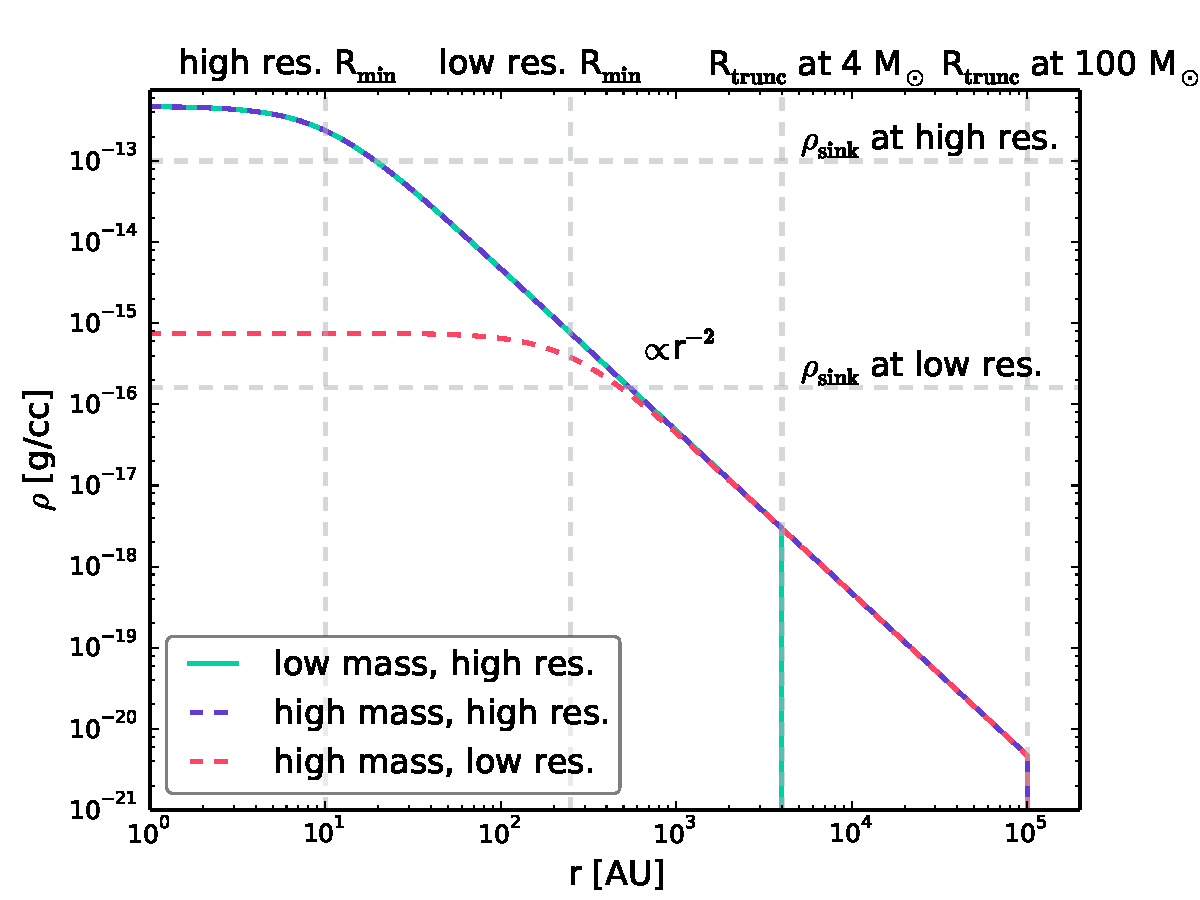
\includegraphics[width=0.85\textwidth]{Figures/new_nsis}
 \captionsetup{justification=justified,singlelinecheck=false,width=\linewidth}
 \decoRule
 \caption[Singular isothermal sphere profile]{The singular isothermal sphere profiles: The turquoise line shows the particular singular isothermal sphere profile of the low mass setup.
                                              The dashed lines in blue/red show the initial conditions for high mass spheres of 100 M$_{\odot}$.
                                              Radius parameters R$_{min}$ limit the central core densities and adjust the maximal resolutions of the collapse simulations.
                                              They were set to 10 AU for high resolution and 250 AU for low resolution.
                                              Truncation radii $R_{trunc}$ were set to 4000 AU and 0.485 pc, for low and high mass spheres respectively.}
\label{fig:nsis}
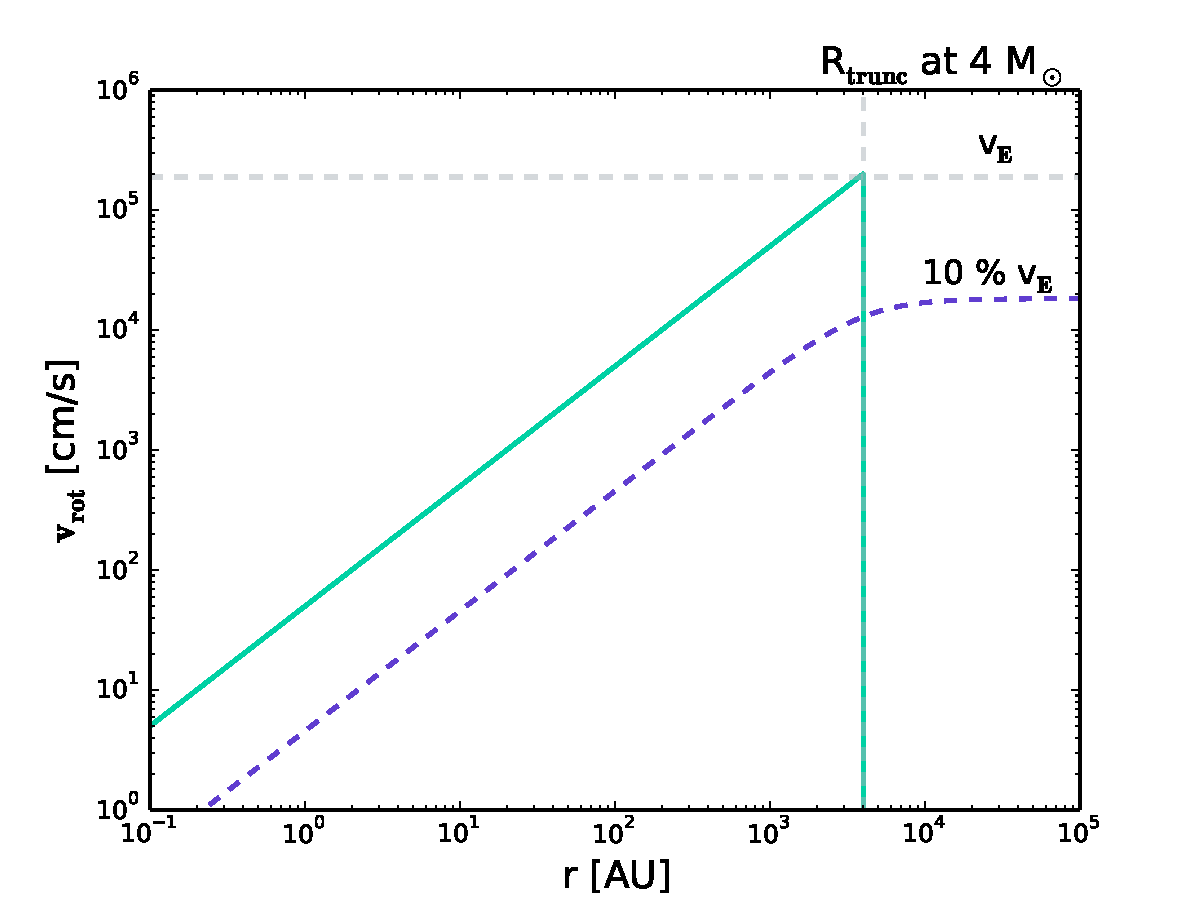
\includegraphics[width=0.85\textwidth]{Figures/solid_rot}
\captionsetup{justification=justified,singlelinecheck=false,width=\linewidth}
\decoRule
\caption[Rotational velocity profile]{The rotational velocity profiles: This plot shows the absolute of rotation velocities in the z=0--plane.
                                      Such a profile was used for all the runs with a mass of $4\,M_{\odot}$ and a truncated radius of $R_{trunc}=4000\,\text{AU}$.
                                      $v_{E}$ is the escape velocity, which is the minimal velocity an object needs to break free of the gravitational potential of the orbited central body.
                                      Later on, when the high--mass isothermal sphere collapses were investigated, these rotation profiles had to be changed for bigger spheres in order to avoid unrealistically high velocities.
                                      The velocity profiles were therefore smoothly connected to a value of 10 \% of the escape velocity and kept constant throughout the rest of the spheres.}
\label{fig:rot_vel}
\end{figure}
\FloatBarrier


%\newpage
% Reference runs ----------------------------------------------------------------------------------------
\section{Reference runs}
\label{sec:Reference_runs}

Pure--hydrodynamical simulations build a base line, to which the simulations including radiative transfer can be compared.
For all such simulations a polytropic equation of state was implemented; see \figref{fig:isotropic_hack}.
Of course, this equation of state is inspired by the behavior expected in star formation.
This allows the simulations to mimic the formation of the first Larson core where the medium becomes optically thick to radiation and consequently heats up without actually including radiative transfer.
In the low--resolution simulations however, the sink density threshold had to be lowered to account for the low resolution, which made them effectively isothermal.
For those runs that could resolve the Jeans length at the opacity limit, the temperature climbed to maximally 16 K.

Since this method is based on an idealized model, the first phase during the collapse maintains a very symmetric fragmentation pattern of which the \code{scaled\_up\_isoknee\_sink} run shows a nice example in \figref{fig:isotropic_binaries}.
Although some of the simulations produced expected behavior such as very symmetric binary--like fragmentation patterns, this indirect method of modeling star formation is not realistic.

Other reference simulations have been also performed and can be found in the same Table \ref{tab:hydro_pure}, all with \code{rt=.false.}
Some of them were evolved for so long that the rotating disk is totally destroyed by fragmentation.

The disks in purely--hydrodynamical simulations start to fragment due to the fact that without radiation the gas cannot reach high enough temperatures to prevent fragmentation and there are no steady, opposing forces to keep gravity at bay.
Thus, the results are very high sink particle numbers with low masses on average.
After around 100 kyrs, all pure--hydrodynamical simulations have converted at least 50\% of gas mass into sinks.

\begin{figure}[!htb]
 \centering
 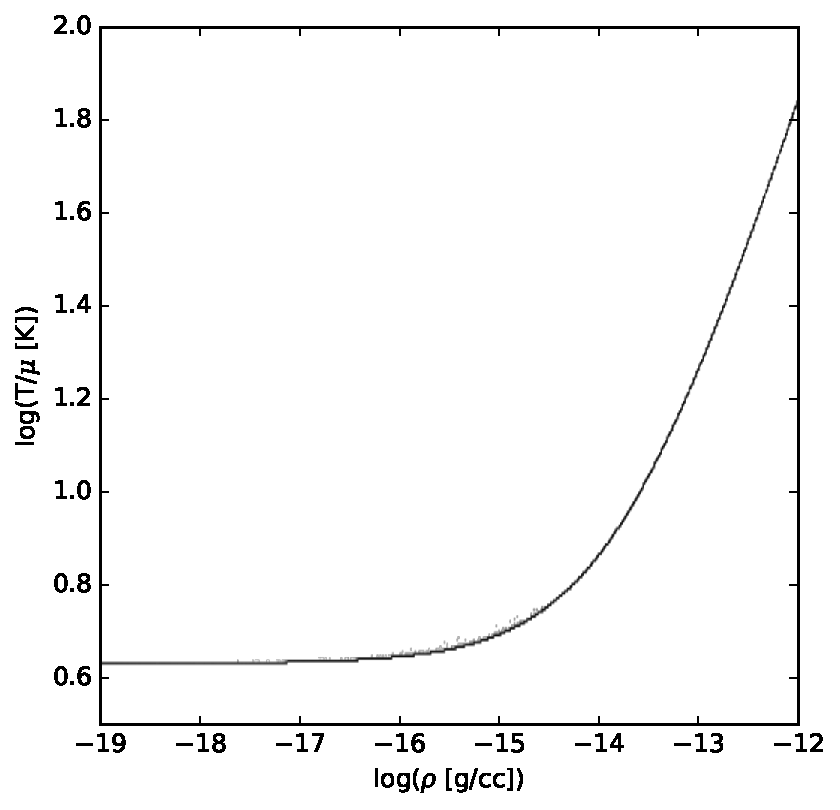
\includegraphics[width=0.8\textwidth]{Figures/isotropic_hack}
 \captionsetup{justification=justified,singlelinecheck=false,width=\linewidth}
 \decoRule
 \caption[Polytropic EOS]{The density--temperature phase plot of run \code{scaled\_up\_isoknee\_sink} at around 10.4 kyrs.
                          At the knee density of $10^{-14}$ g/cc the temperature increases quasi--adiabatically.
                          The EOS is the same for all purely--hydrodynamical runs.
                          It presents a poor--mans version of radiative transfer as it imitates the formation of the first Larson core at the opacity limit without actually performing radiative transfer.}
\label{fig:isotropic_hack}
\end{figure}
\FloatBarrier

\begin{figure}[!htb]
 \centering
 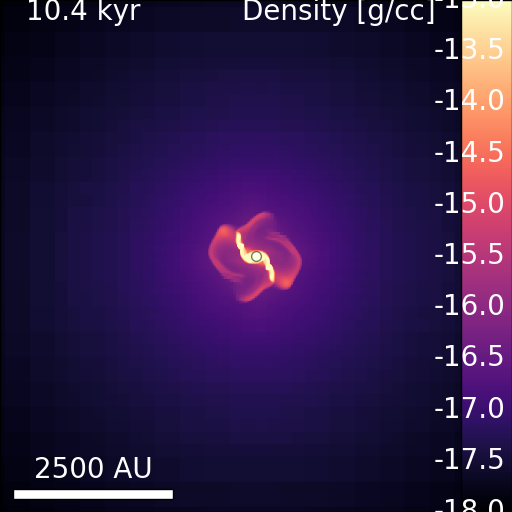
\includegraphics[width=0.6\textwidth]{Figures/isotropic_binaries}
 \captionsetup{justification=justified,singlelinecheck=false,width=\linewidth}
 \decoRule
 \caption[Fragmentation pattern]{A single snapshot of run \code{scaled\_up\_isoknee\_sink} which is a high--resolution, high--mass run.
                                 The symmetrical fragmentation patter is similar to those observed by \citet{Commercon_binaries}.
                                 This confirms the purely--hydrodynamical simulations and validates their use in comparison with radiation hydrodynamics simulations later.}
\label{fig:isotropic_binaries}
\end{figure}
\FloatBarrier

The reference runs also show another interesting feature which was already predicted in \secref{subsec:Instabilities}.
The self--similarity of the profile of a singular isothermal sphere implies that free--fall of matter towards the center is always steady.
\figref{fig:smaccm_selfsim} shows only one of many confirmations that isothermally collapsing cores are accreting with a constant rate of $\dot{M}_{acc} \sim \frac{c_{s}^{3}}{G}$.
During the whole simulation, the accretion rate seems to be fairly steady until most of the gas has been consumed and the sink reaches a maximal mass.

\begin{figure}[!htb]
 \centering
 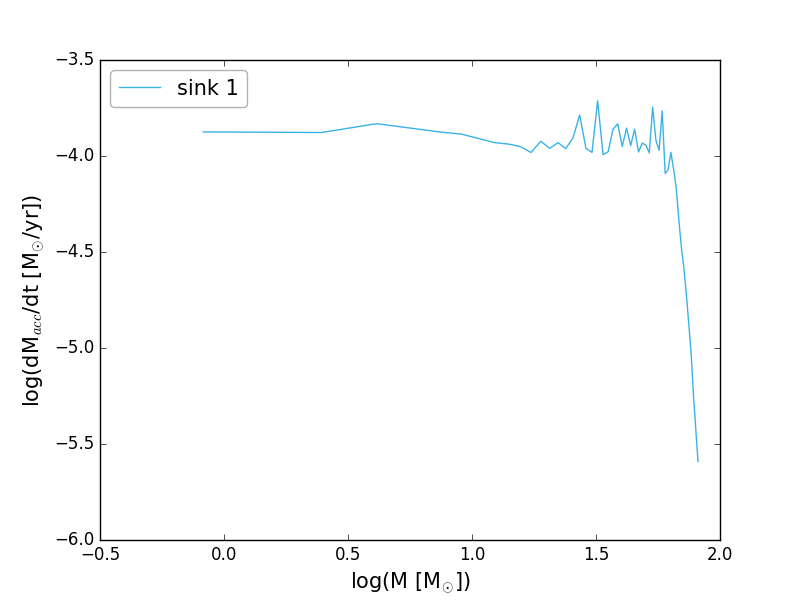
\includegraphics[width=0.75\textwidth]{Figures/smacc_m_selfsim_merge}
 \captionsetup{justification=justified,singlelinecheck=false,width=\linewidth}
 \decoRule
 \caption[Sink accretion rate plot of a pure--hydrodynamics run]{Accretion rate plot of the most massive sink formed in the high--mass low--resolution simulation \code{self\_similar\_iso\_merge}.
                                                                 Due to the isothermal sphere collapse, the accretion rate is steady at around $10^{-4}$ M$_{\odot}$ per year.
                                                                 Once most of the gas mass is consumed, the sink mass settles at a final value.}
\label{fig:smaccm_selfsim}
\end{figure}
\FloatBarrier

%\newpage
% Core collapse simulations - Comparison of HD with RHD ----------------------------------------------------------------------------------------
\section{Disk fragmentation}
\label{sec:Idealized_core_collapses}

For all variants of initial conditions (low--mass high--resolution, high--mass high--resolution, and high--mass low--resolution simulations) pure--hydrodynamics as well as radiation hydrodynamics simulations have been conducted.

\figref{fig:hydro_purePt2} shows snapshots of such a reference simulation, in which the low--mass, high--resolution initial conditions were used.
The excessive fragmentation can clearly be seen in the second panel on the left side.
Further details can be found in the overview in Appendix~\ref{sec:Overview} in Table \ref{tab:hydro_pure} under \code{ref\_run}.

In \figref{fig:rhd_snapshots} the same simulation with radiation can be seen.
The differences of both are enormous.
While in the reference run the disk already totally fragmented after 20 kyrs and formed many low mass sink particles, the simulation with radiation formed only one massive sink in the center of a fairly stable disk.

The need for radiation hydrodynamics is not just evident by this problem mentioned above.
Fragmentation of isothermal, hydrodynamical collapse simulations is excessive and produces too many sink particles.
To show and analyze the difference between pure--hydrodynamics and radiation hydrodynamics simulations, we introduce the \textit{Toomre parameter}

\begin{equation}
  Q = \frac{\omega c_{s}}{\pi G\Sigma}
\end{equation}

where $\omega$ is the epicyclic frequency of the central sink, $c_{s}$ the local sound speed in the gas and $\Sigma$ the surface density of the disk.
The Toomre criterion states that for $Q>1$ the disk can be considered stable against further collapse, whereas for $Q<1$ it is unstable.

It combines the parameter to express the balance between radiation, rotation and gravity.
The parameter $\omega$ describes the orbital frequency of the sink produced by rotation.
The greater the rotational velocity is, the more stable the disk is against gravitational collapse.
If $\omega$ increases, so does the Toomre parameter.
Radiation is another component opposing gravity.
$c_{s}$ is proportional to the temperature of the gas.
Accordingly, if the disk heats up and increases $c_{s}$ due to either internal friction or radiation, $Q$ increases.
The surface density term $G\Sigma$ incorporates the gravitational strength and tendency of the disk to collapse.

The criterion also indirectly represents a trend of the disk to regulate and stabilize itself.
If $Q<1$, the gravitational collapse proceeds and $\Sigma$ increases.
However, in this case there is more mass for the sink to accrete in the center.
Since the radiation emitted at the sink, the accretion luminosity, is proportional to the mass, the radiation subsequently increases also.
The parameter $c_{s}$ therefore increases and works towards the stabilization of the disk.

The Toomre parameter analysis for the collapsed disks of the low--resolution and high--resolution simulations reveals interesting properties.
\figfigref{fig:Toomre_hydro}{fig:Toomre_rt} show Toomre profiles of two runs with the mere difference that one of them is purely--hydrodynamical (not radiative transfer, simply a polytropic EOS), while the other involves radiative transfer.
In the comparison of both, it can be seen that the run with radiative transfer is more stable, especially in the range of radii for which the pure--hydrodynamical simulations tend to be unstable.
In fact, this is a trend detectable with all self--similar and scaled--up runs for which a pure--hydrodynamical and radiative transfer version was performed.
In the region where the central sink heats up the gas by irradiating it in the infrared spectrum, the Toomre parameter is raised and therefore the disk around the sink tends to be more stable.

This is also recognizable in the direct snapshots of the simulations in \figfigref{fig:hydro_purePt2}{fig:rhd_snapshots}, each on the left side of the second panel.
There, the influence of radiation can be observed through the gas' appearance.
Though radiation the gas' temperature rises, appears therefore more diffuse, and does not collapse to filaments and clumps at all or not as fast as in pure--hydrodynamics simulations.

\begin{figure}[!htb]
 \centering
 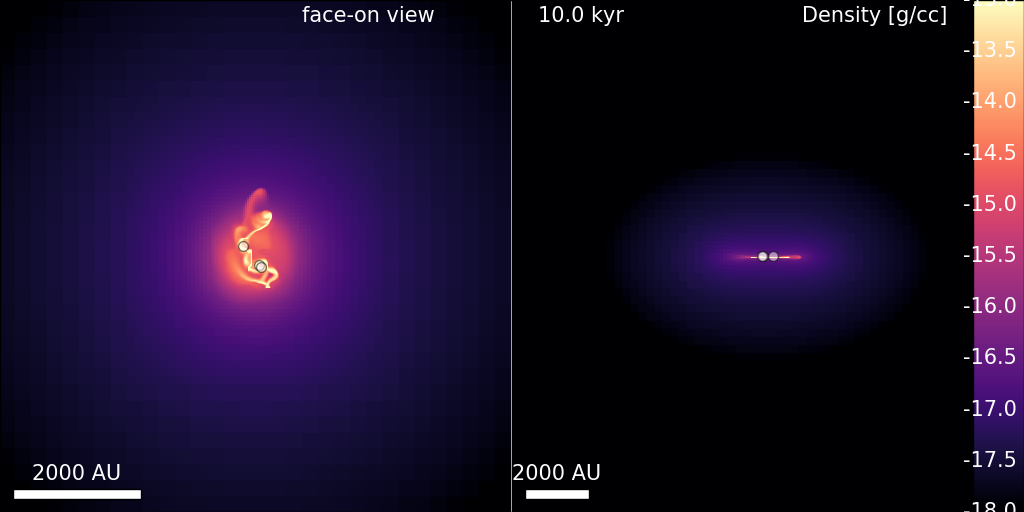
\includegraphics[width=0.95\textwidth]{Figures/hydro_pure/pure_hydro_1}
 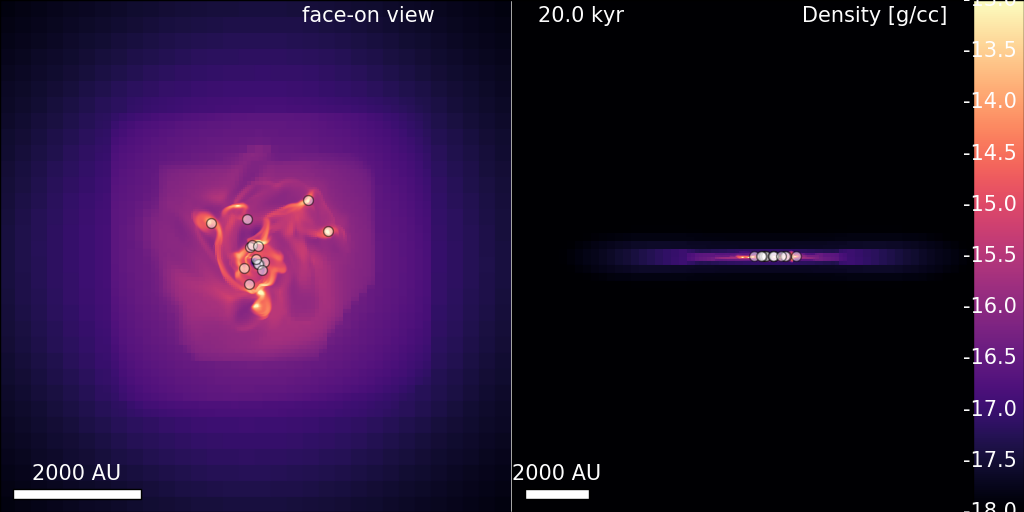
\includegraphics[width=0.95\textwidth]{Figures/hydro_pure/pure_hydro_2}
 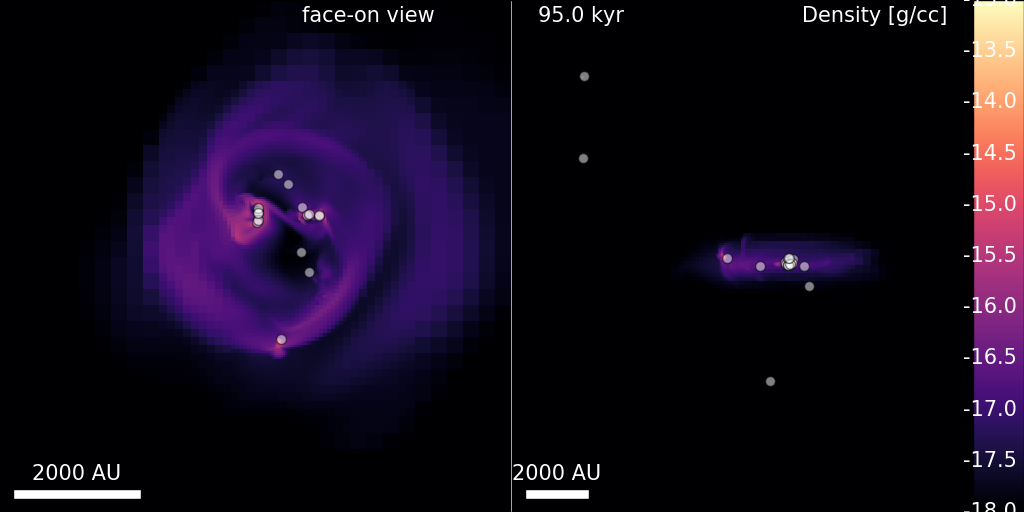
\includegraphics[width=0.95\textwidth]{Figures/hydro_pure/pure_hydro_3}
 \captionsetup{justification=justified,singlelinecheck=false,width=\linewidth}
 \decoRule
 \caption[Hydrodynamical isothermal sphere collapse]{Snapshots of a high--resolution, low--mass pure--hydrodynamics reference run \code{ref\_run}.
                                                     Its initial conditions correspond to a rotating singular isothermal sphere profile as described in \secref{subsec:Initial_conditions}.
                                                     The right side of each panel shows the formation of a disk due to the angular momentum of the gas while falling onto the sink which was formed in the beginning.
                                                     Fragmentation sets in almost immediately after the formation of the first sink as there are no opposing forces against gravity.
                                                     The result is a very turbulent disk with a high sink formation rate.}
\label{fig:hydro_purePt2}
\end{figure}
\FloatBarrier

\begin{figure}[!htb]
 \centering
 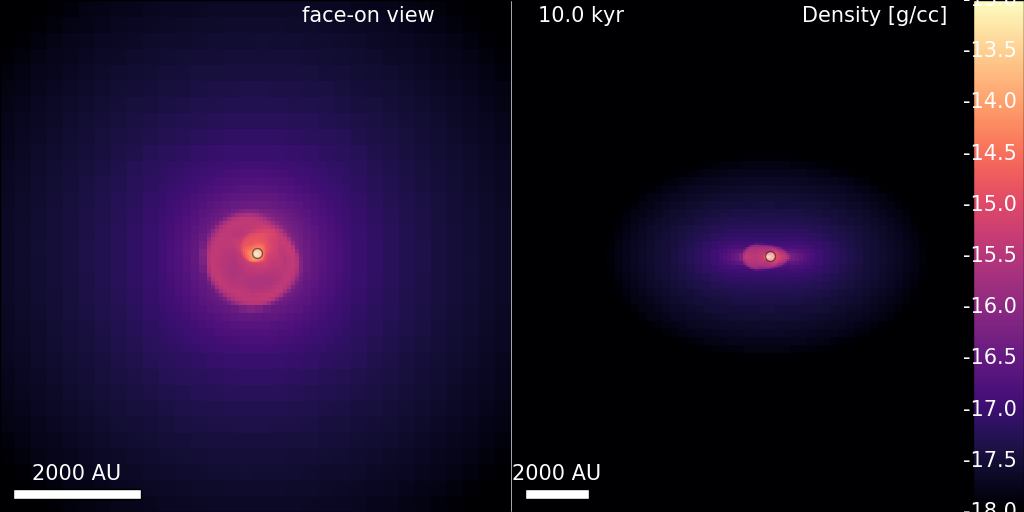
\includegraphics[width=0.95\textwidth]{Figures/rhd/multi_00039}
 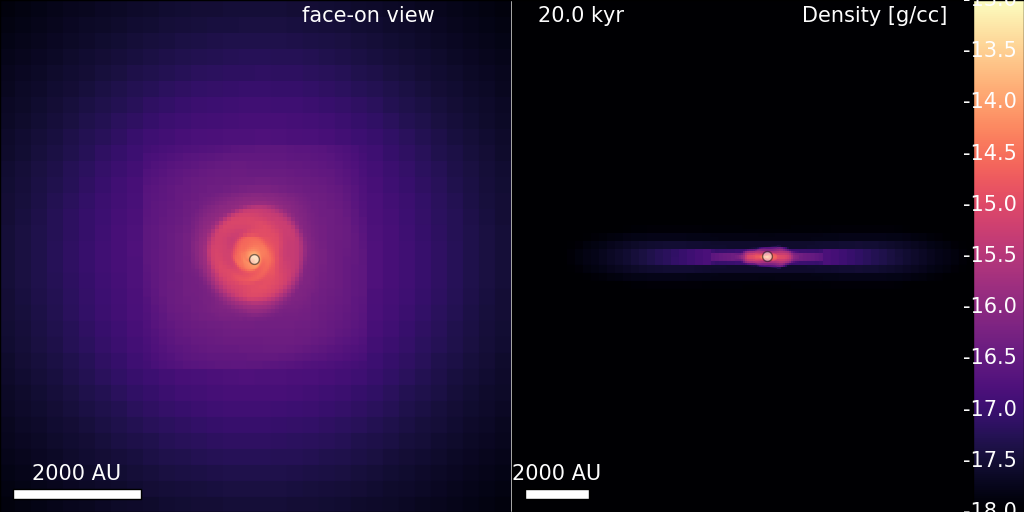
\includegraphics[width=0.95\textwidth]{Figures/rhd/multi_00079}
 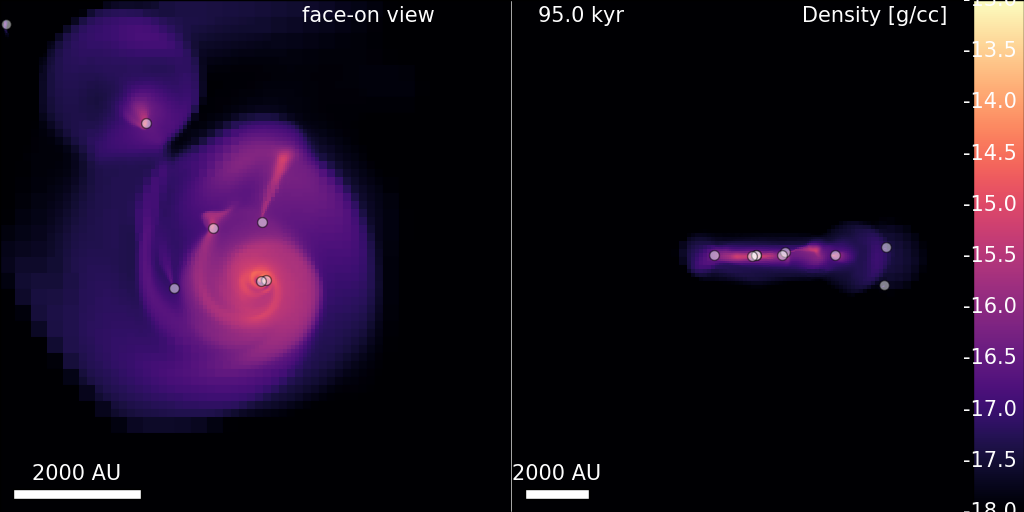
\includegraphics[width=0.95\textwidth]{Figures/rhd/multi_00379}
 \captionsetup{justification=justified,singlelinecheck=false,width=\linewidth}
 \decoRule
 \caption[Radiation hydrodynamical sphere collapse]{Snapshots of a high--resolution, low--mass radiation hydrodynamics run \code{nsub\_const\_rtc}.
                                                    This run's only difference to the one in \figref{fig:hydro_purePt2} is that radiative transfer is included.
                                                    In comparison of both, we see that here the resulting disk is thicker and its gas smoother due to the heat induced by the infrared radiation from the central sink.
                                                    Fragmentation only happens far from the central sink where the radiation has not heated the gas.
                                                    These fragments form sinks and return to the center due to dynamical friction and the gravitational attraction of the central sink.
                                                    This is easily noticeable in the last panel as wakes tracing the sinks' paths.}
\label{fig:rhd_snapshots}
\end{figure}
\FloatBarrier


\begin{figure}[!htb]
 \centering
 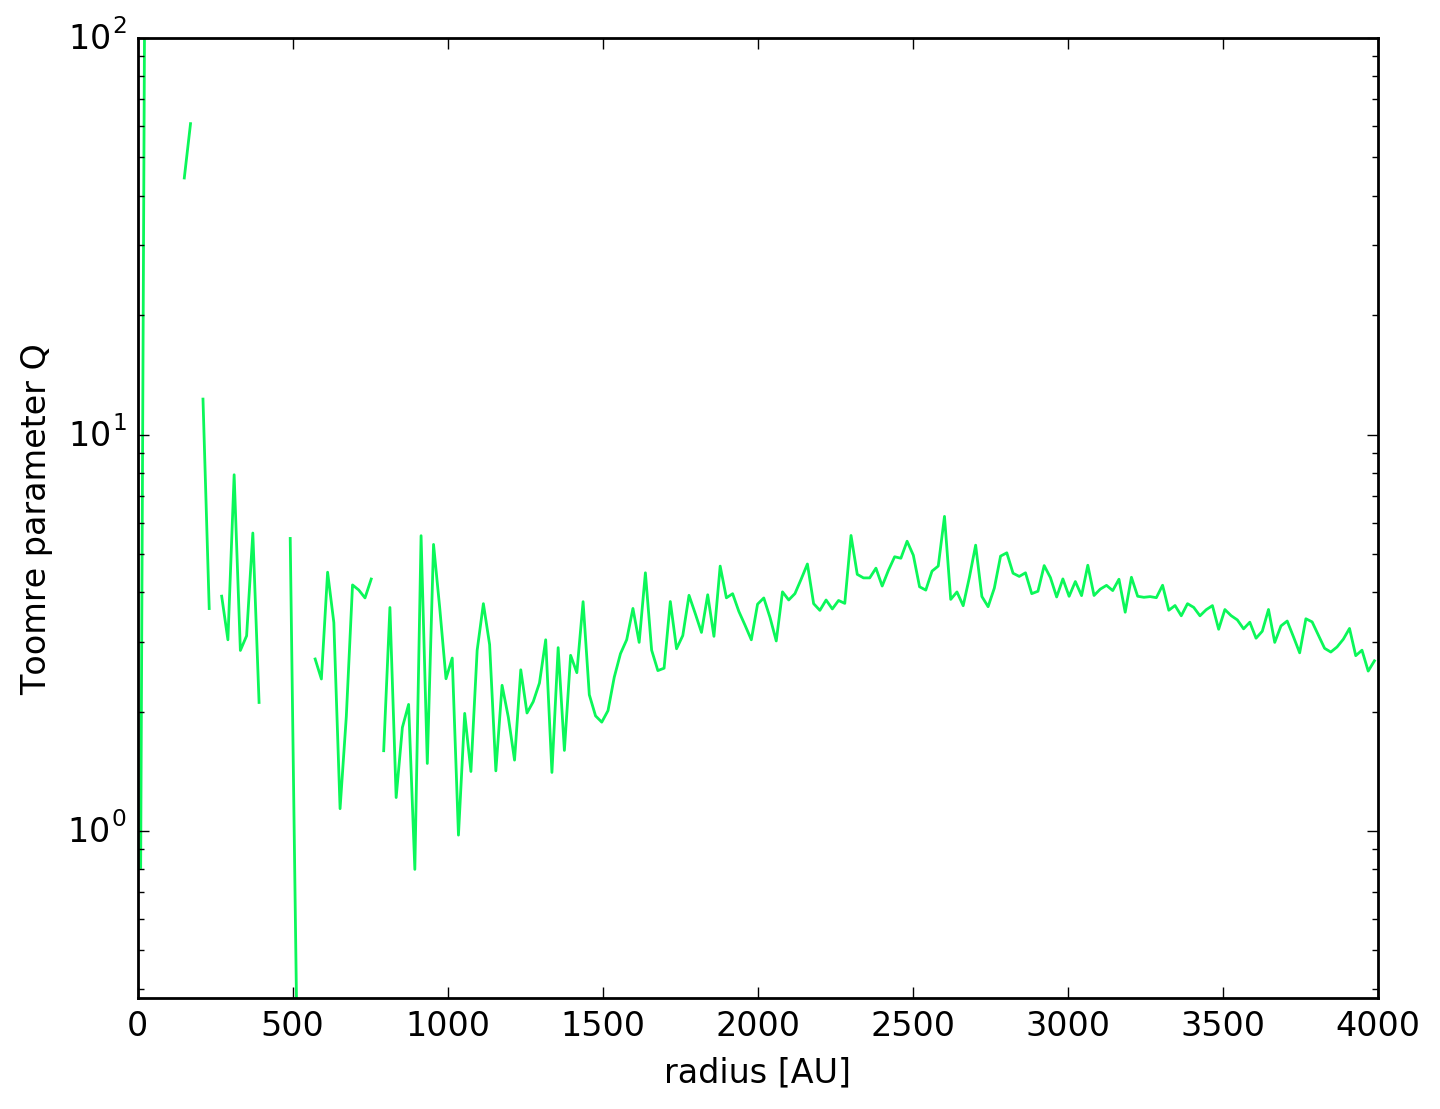
\includegraphics[width=0.85\textwidth]{Figures/toomre_hydro}
 \captionsetup{justification=justified,singlelinecheck=false,width=\linewidth}
 \decoRule
 \caption[Toomre profile of a pure--hydrodynamics run]{A Toomre profile of run \code{self\_similar\_iso\_merge}, a high--mass low--resolution simulation at a time of 1.24 Myrs, centered around the most massive sink.
                                                       It is a purely--hydrodynamical simulation, which showed a high degree of fragmentation.
                                                       It shows a tendency of gravitational instability around the radii between 500 and 1000 AU.}
\label{fig:Toomre_hydro}
\end{figure}
\FloatBarrier

\begin{figure}[!htb]
 \centering
 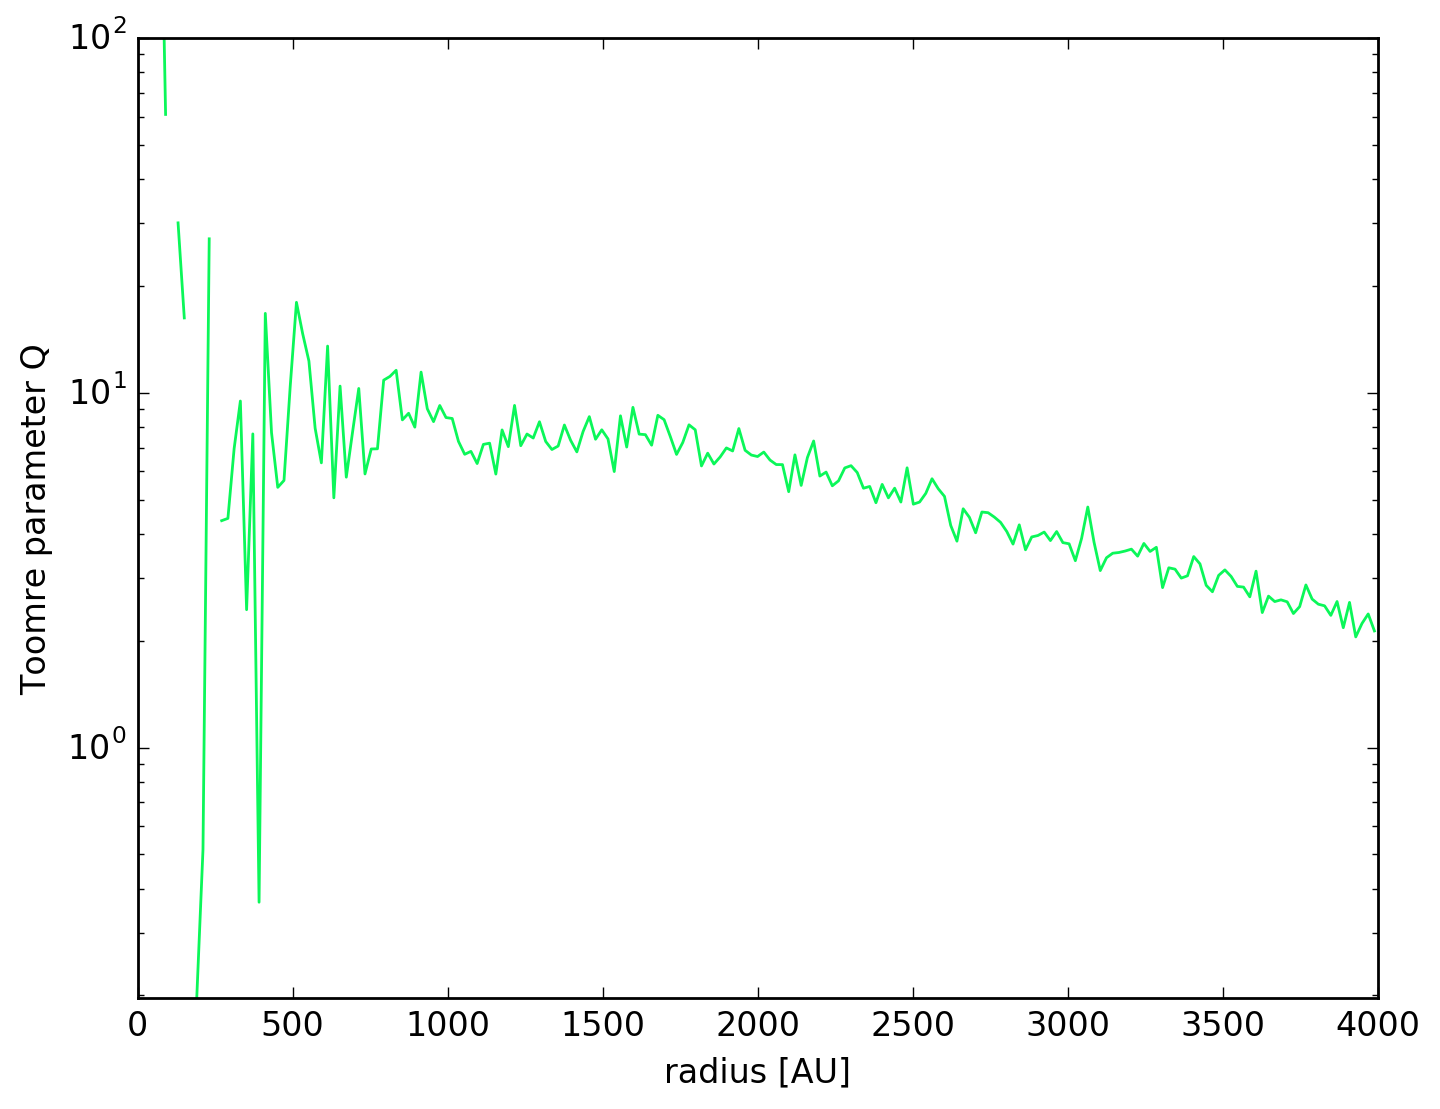
\includegraphics[width=0.85\textwidth]{Figures/toomre_rt}
 \captionsetup{justification=justified,singlelinecheck=false,width=\linewidth}
 \decoRule
 \caption[Toomre profile of a radiative transfer run]{A Toomre profile of run \code{self\_similar\_merge}, a high--mass low--resolution simulation at a time of 1.24 Myrs, centered around the most massive sink.
                                                      The same initial conditions were implemented as for the run in \figref{fig:Toomre_hydro} with the exception that this simulation included radiative transfer.
                                                      When compared to the previous \figref{fig:Toomre_hydro}, most of the values of $Q$ are clearly above 1, indicating gravitational stability.}
\label{fig:Toomre_rt}
\end{figure}
\FloatBarrier


%\newpage
% Cloud simulation----------------------------------------------------------------------------------------
\section{Molecular cloud}
\label{sec:MC}

Having thoroughly tested the numerical and physical influence of radiation onto an astrophysical fluid, the initial conditions for an entire molecular cloud simulation were prepared.

In the evaluation of the previous tests, especially of the runs' duration, it was deemed unnecessary to utilize the implementation of variable speed of light, since there is almost no speed--up, and in some cases it even prolonged the simulations.
However the subcycling of the RT routines seemed to provide a considerable gain in simulation speed without a grave loss in accuracy.
Again, only infrared radiation was used in the simulation.
Hence, the parameters of the radiative transfer module were calibrated such that the radiation travels at a constant fraction of the actual speed of light.

The RSL was calculated according to \citet{Skinner_Ostriker}.
They calculated the reduced speed of light depending on the maximum of the initial turbulent velocity dispersion $\sigma$, the sound speed $c_{s}$ and the optical depth of the initial uniform cloud $\tau$.

\begin{equation}
  \tilde{c} \geq (\sigma + c_{s})\mathrm{max}(\tau, 1) \qquad\quad \text{with} \quad \tau\equiv\frac{3}{2}\kappa_{P}\Sigma_{cloud}
\label{eq:Skinner_Ostriker_RSLA}
\end{equation}

where $\Sigma_{cloud}$ is the surface density of the initial cloud configuration determined by its mass M$_{cloud}$ and radius R$_{cloud}$.
The initial total gas mass of the cloud amounted to around M$_{cloud} \sim 2.4\times10^{4}$ M$_{\odot}$.
This mass was distributed in a spherical configuration with radius R$_{cloud} \sim 5$ pc.
The calculation of the optical depth for these parameters suggests that the global initial state of the cloud is quite far in the optically thin regime.
Therefore, the opacity limit $\tau = 1$ was applied in the approximation of the reduced speed of light.
The proportionality constant in the previous relation can be adjusted to the simulation.
In our case, a factor of 10 was used to stay on the more conservative side in the approximation.

Since highly turbulent gas flows are observed in almost all molecular clouds, they are a key component in such cloud simulations.
For this purpose, the sphere of mass M$_{cloud}$ and radius R$_{cloud}$ was actually carved out from another simulation and restarted.
In that simulation, the velocity field was driven by Gaussian random perturbations with a standard Kolmogorov power spectrum $E(k) \propto k^{-5/3}$.
Then, the simulation was run without self--gravity until nice groups of filaments formed, which roughly resemble actual observations of molecular clouds.
At that point, the relevant data within the sphere was saved in grafic--files, which can be read in by RAMSES as initial conditions.

The molecular cloud simulation took several weeks to complete, and even then it only progressed to around 1.5 Myrs.
Still, the simulation results reveal interesting properties.
Further information to some important parameters are listed below, in Table \ref{tab:cloud}.

\begin{table}[!htb]
\begin{adjustbox}{width=\textwidth}
\begin{tabular}{lccccccc}
\toprule
Name ID & rt & hydro\_only & isothermal & sink & scheme & riemann & slope\_limiter \\
\midrule
ir\_cloud & .true. & .false. & .false. & .true. & muscl & hllc & MinMod \\
\bottomrule
\toprule
\quad  & L [pc] & levelmin & levelmax & ncpu & time [Myr] & duration [h] & merging [kyr] \\
\midrule
\quad & 20 & 7 & 13 & 256 & 1.4921 & 384.42 & 5 \\
\bottomrule
\toprule
\quad & N$_{sinks}$ & M$_{tot}$ [M$_{\odot}$] & M$_{sink}$ [M$_{\odot}$] & RSL [km/s] & rt\_nsubcycle & $\kappa_{P}$ [cm$^{2}$/g] & $\kappa_{R}$ [cm$^{2}$/g] \\
\midrule
\quad & 104 & 12885.4389 & 1152.8 & 14.44 & 100 & 0.1 & 0.035 \\
\bottomrule
\end{tabular}
\end{adjustbox}
\captionsetup{justification=justified,singlelinecheck=false,width=\linewidth}
\caption[Cloud simulation parameter info]{Parameter information on the molecular cloud run at the end of the simulation.}
\label{tab:cloud}
\end{table}
\FloatBarrier

\figref{fig:CloudPt3} shows snapshots of the cloud simulation as it progresses.
Rather than displaying the radiation density, it was converted into radiation temperature $T_{rad}$ with
\begin{equation}
  T_{rad} = \Big(\frac{c n_{\gamma} \langle \epsilon \rangle}{c a}\Big)^{1/4}
\end{equation}

where $n_{\gamma}$ is the stored photon number density data, $\epsilon$ the average energy of the particular photon group, $a$ the radiation constant, and $c$ the speed of light.
This makes the radiation temperature comparable to the gas temperature.


\newpage
\thispagestyle{empty}
\begin{figure*}[!htb]
 \centering
 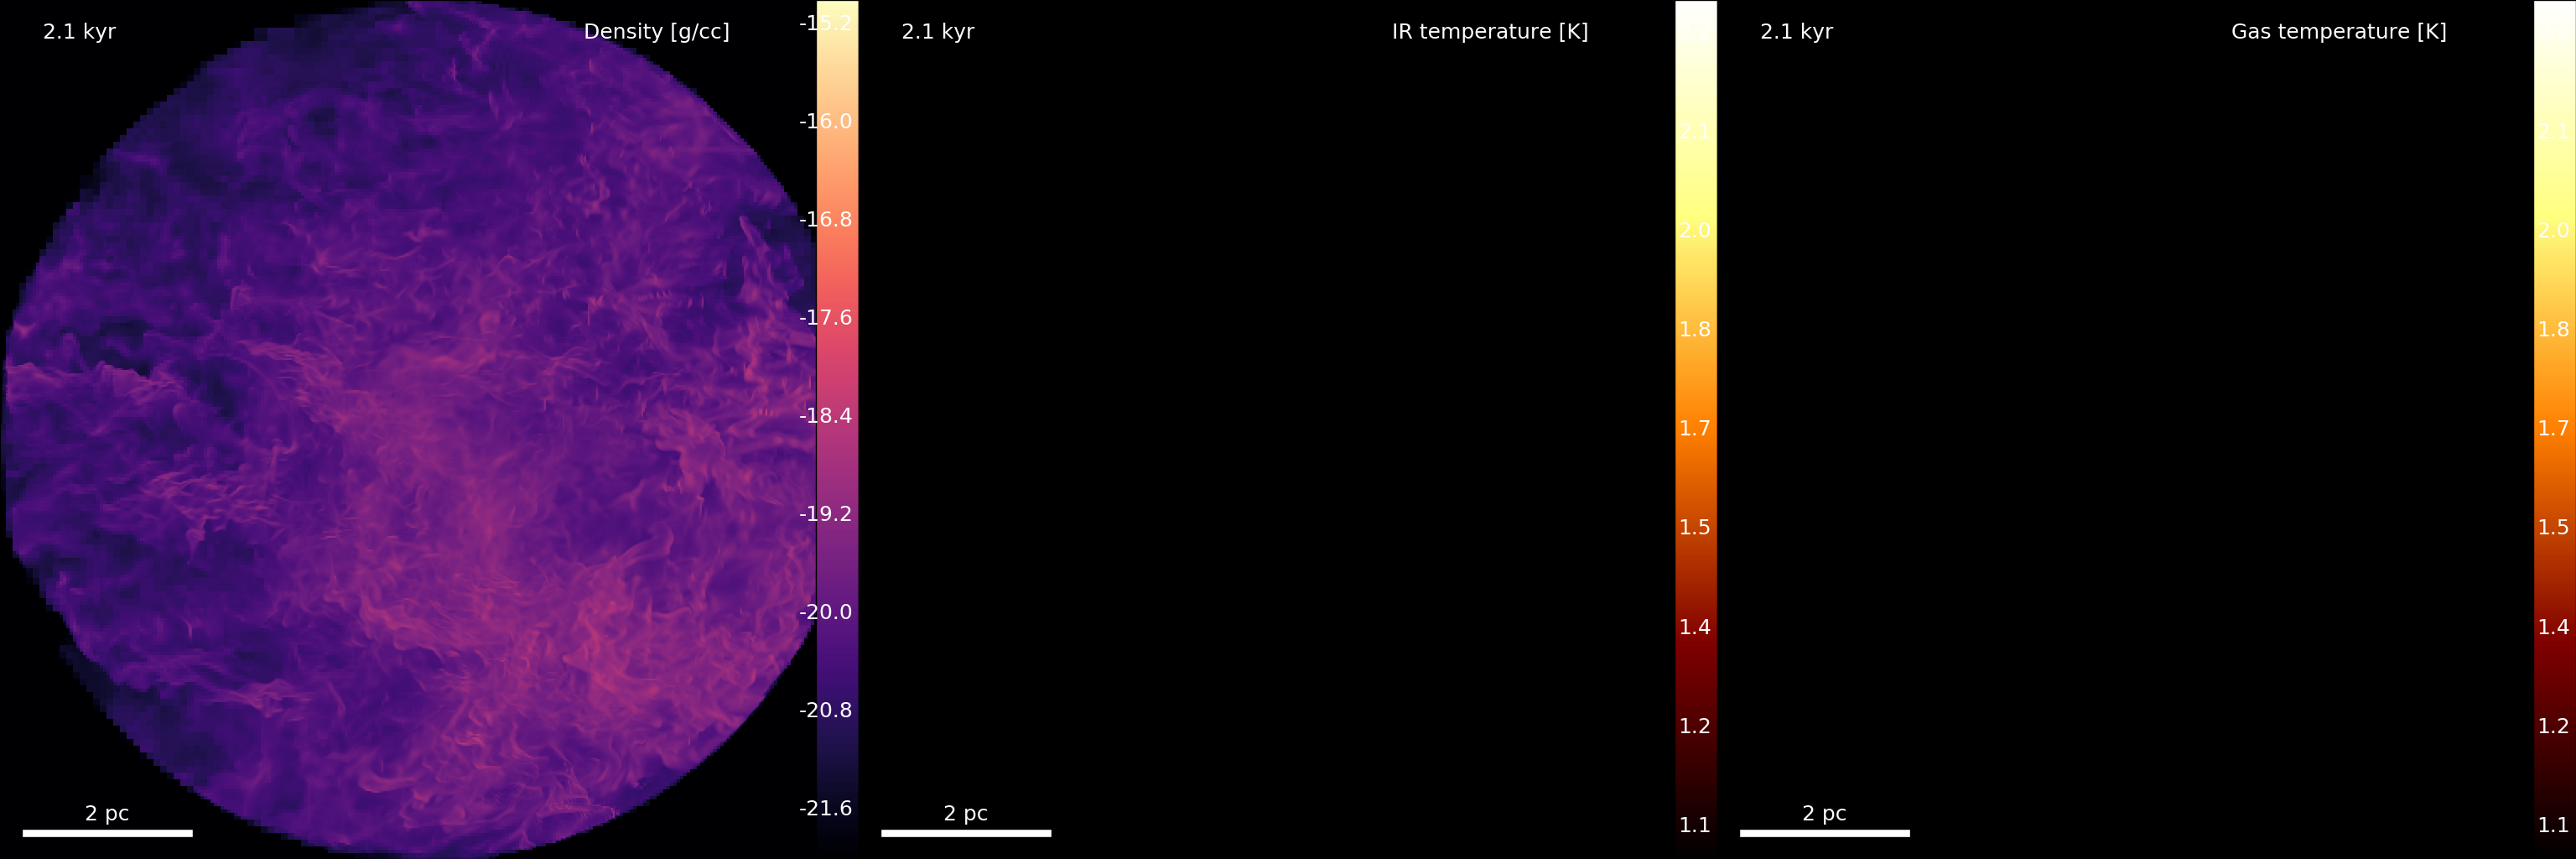
\includegraphics[width=1.05\textwidth]{Figures/cloud_snapshots/multi_00000}
 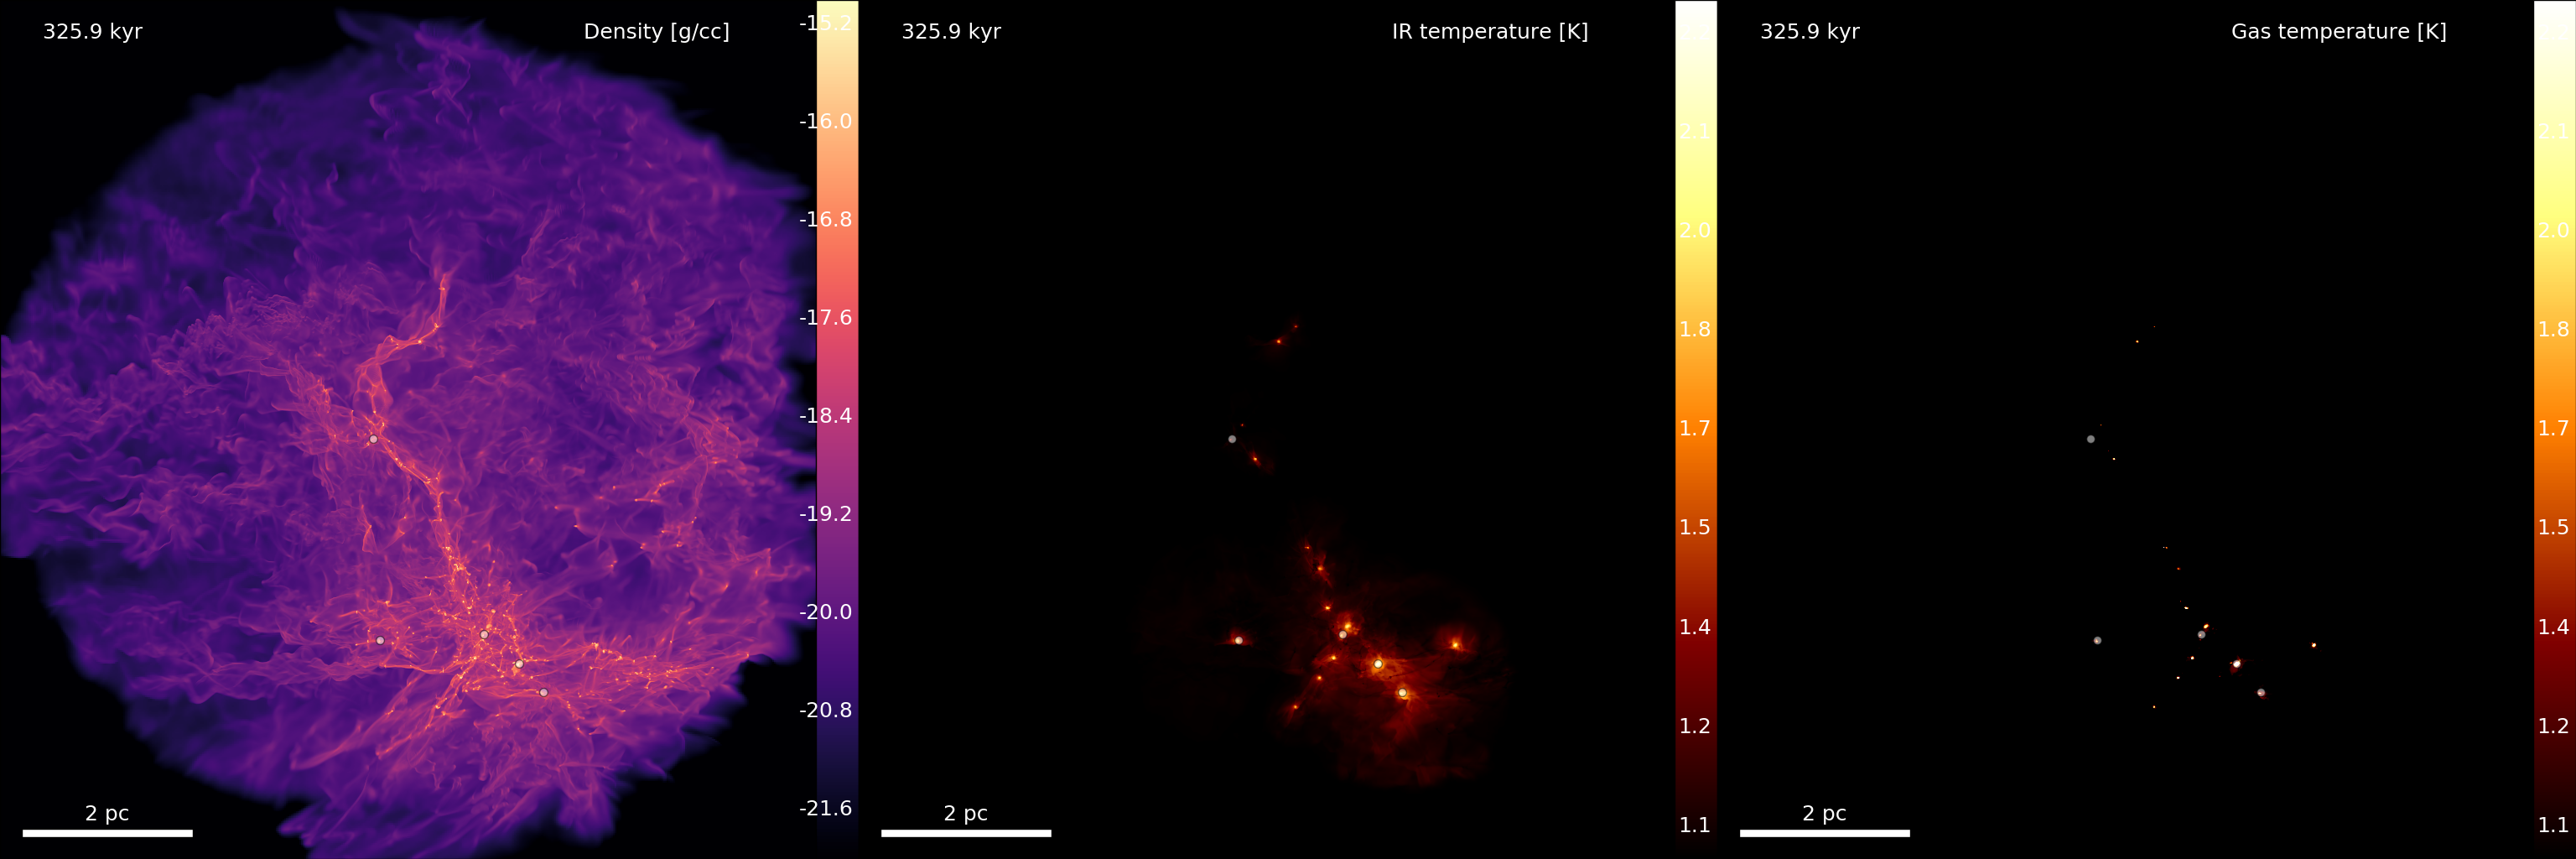
\includegraphics[width=1.05\textwidth]{Figures/cloud_snapshots/multi_00175}
 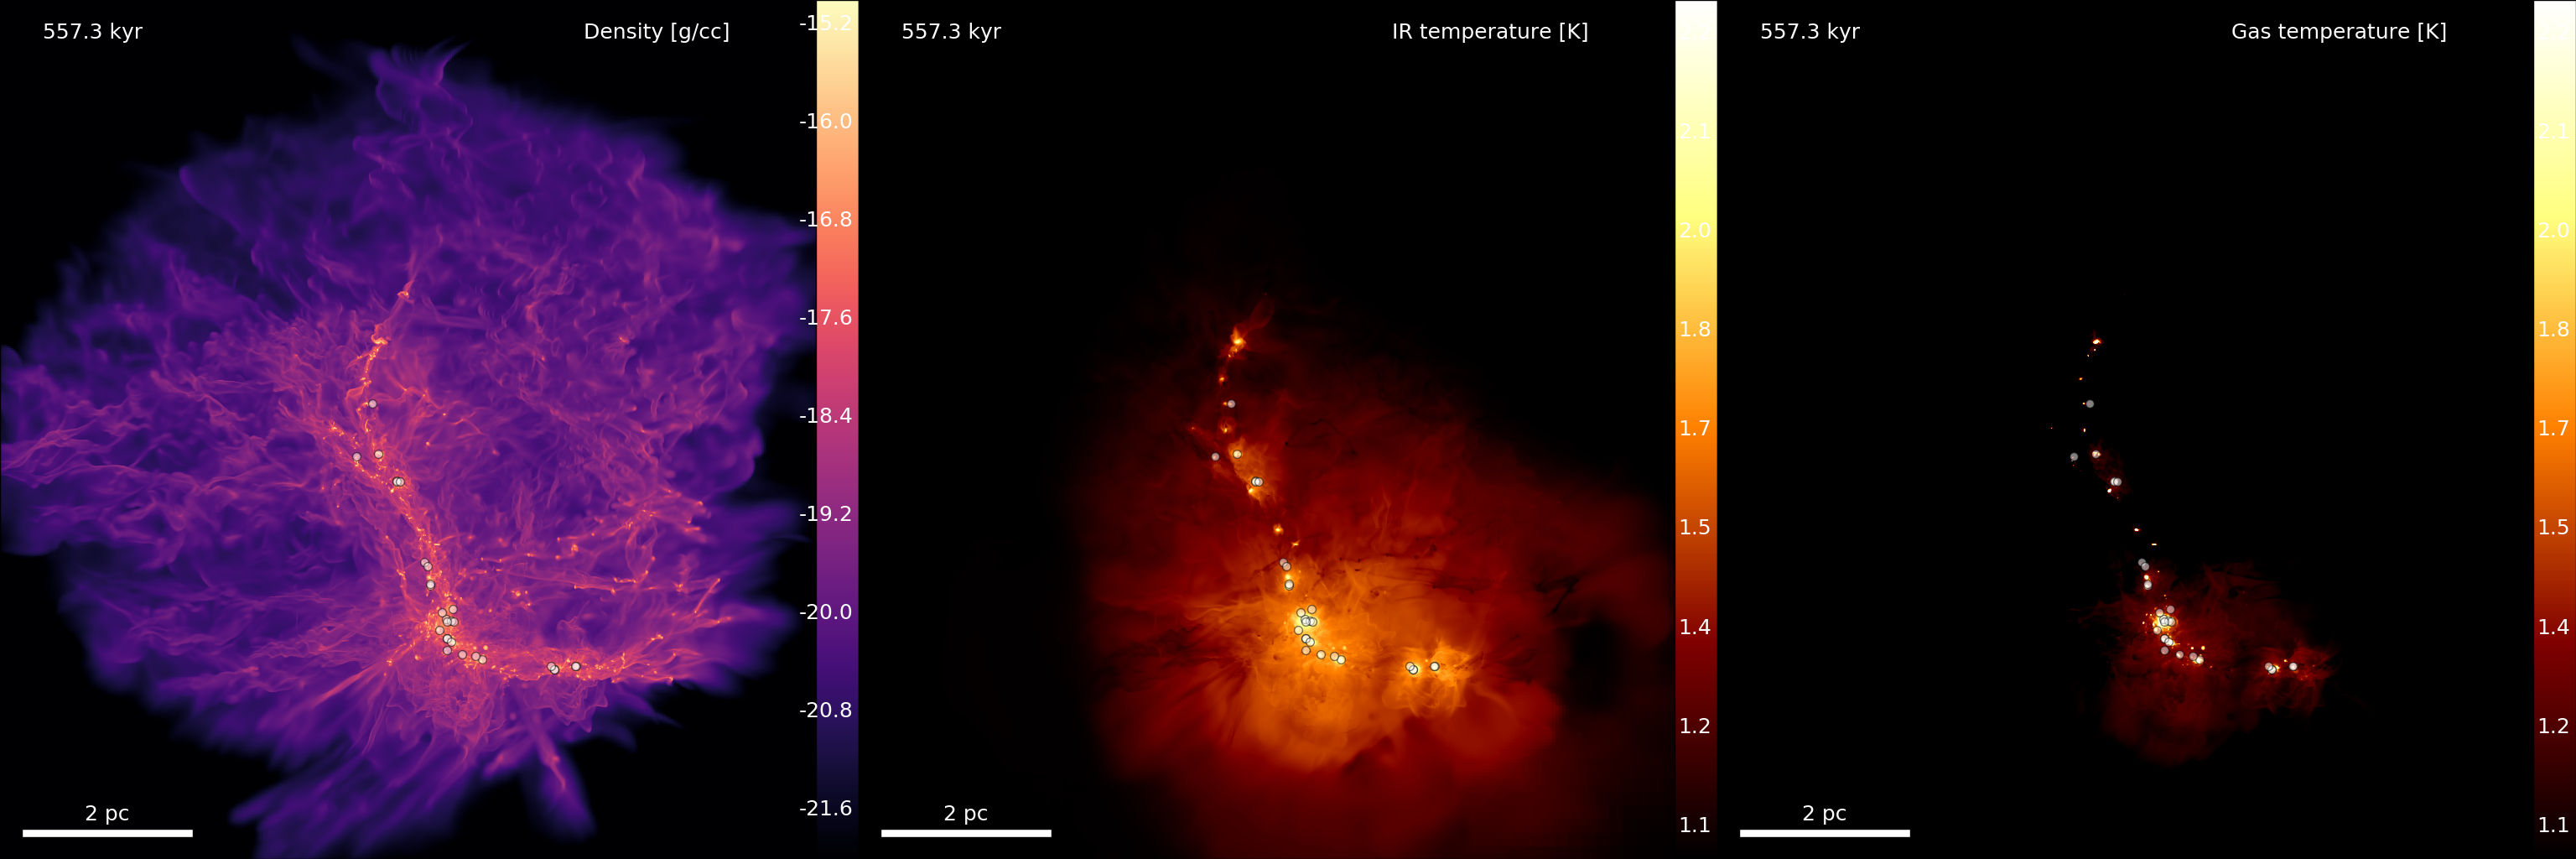
\includegraphics[width=1.05\textwidth]{Figures/cloud_snapshots/multi_00300}
 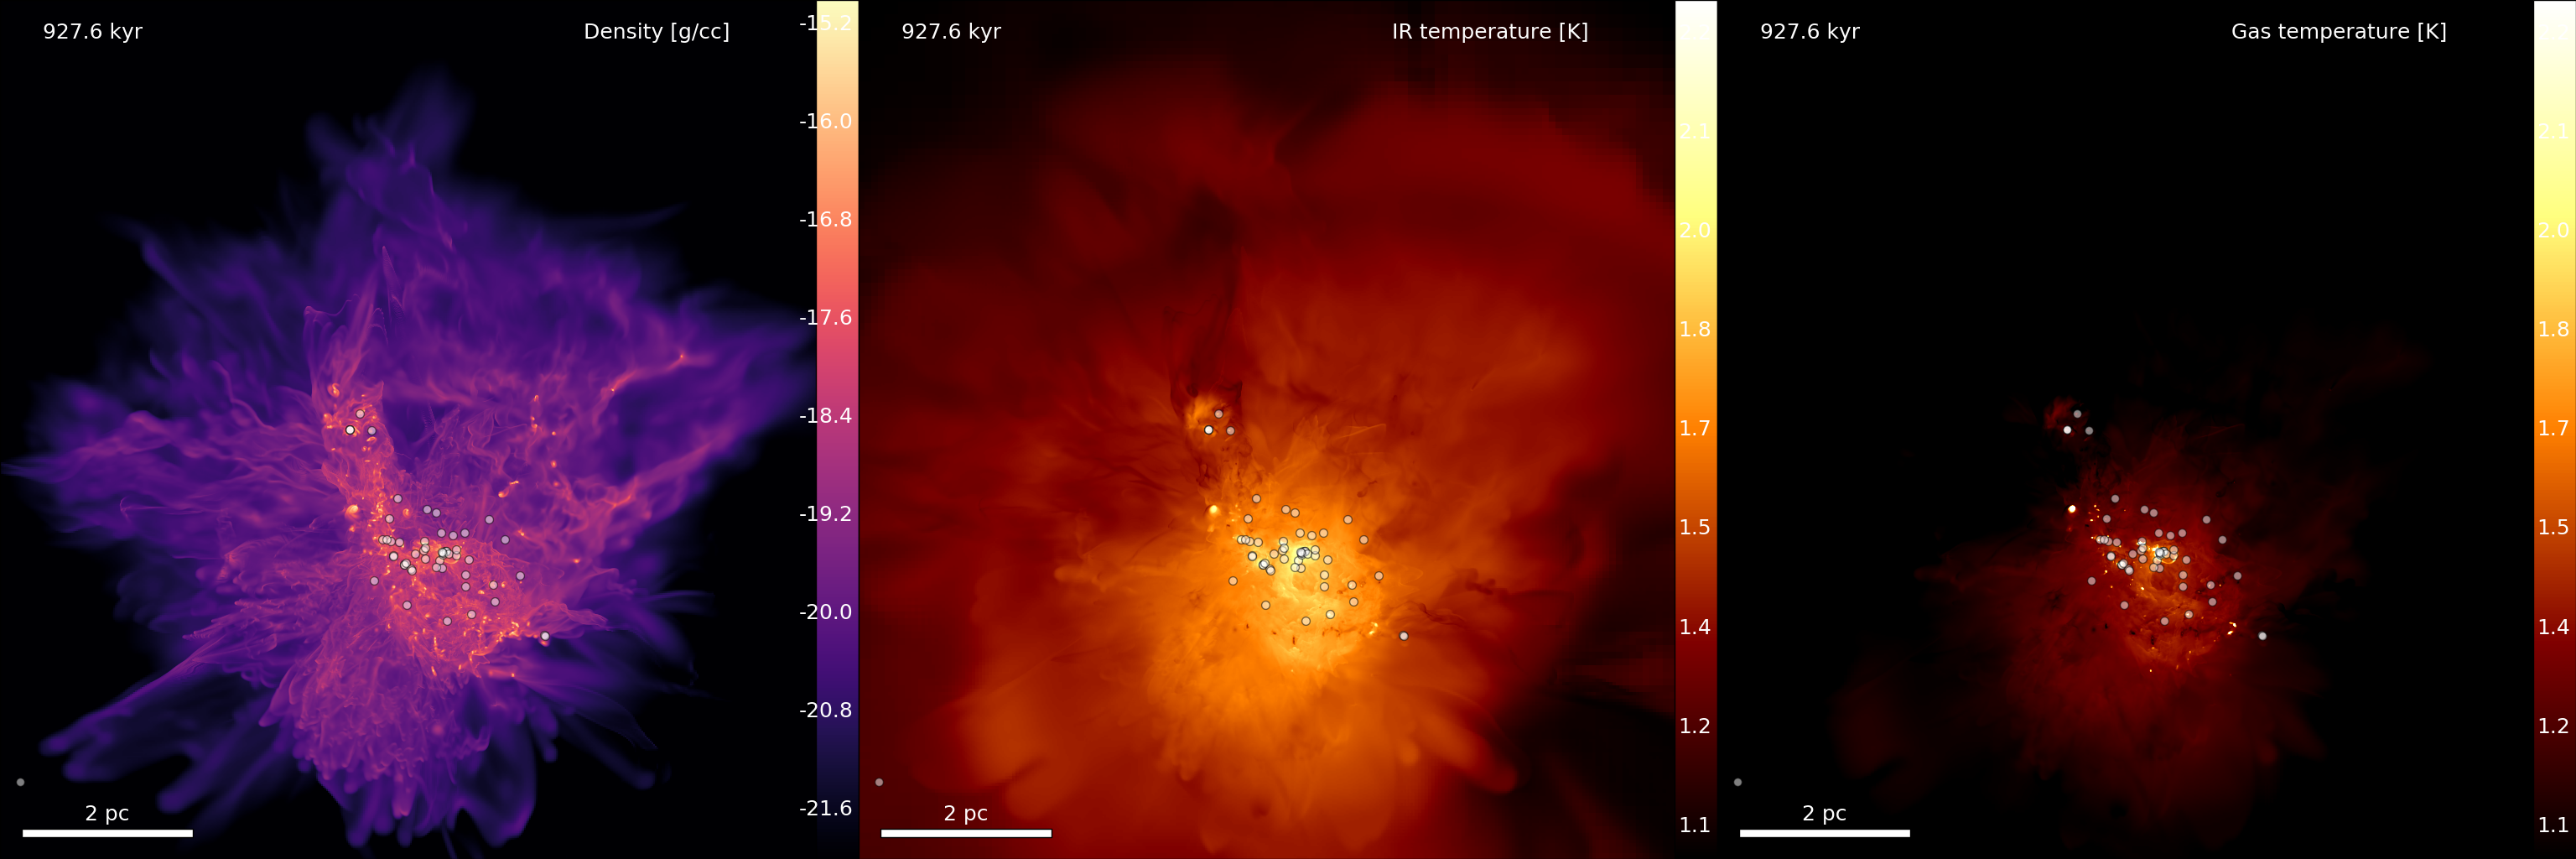
\includegraphics[width=1.05\textwidth]{Figures/cloud_snapshots/multi_00500}
 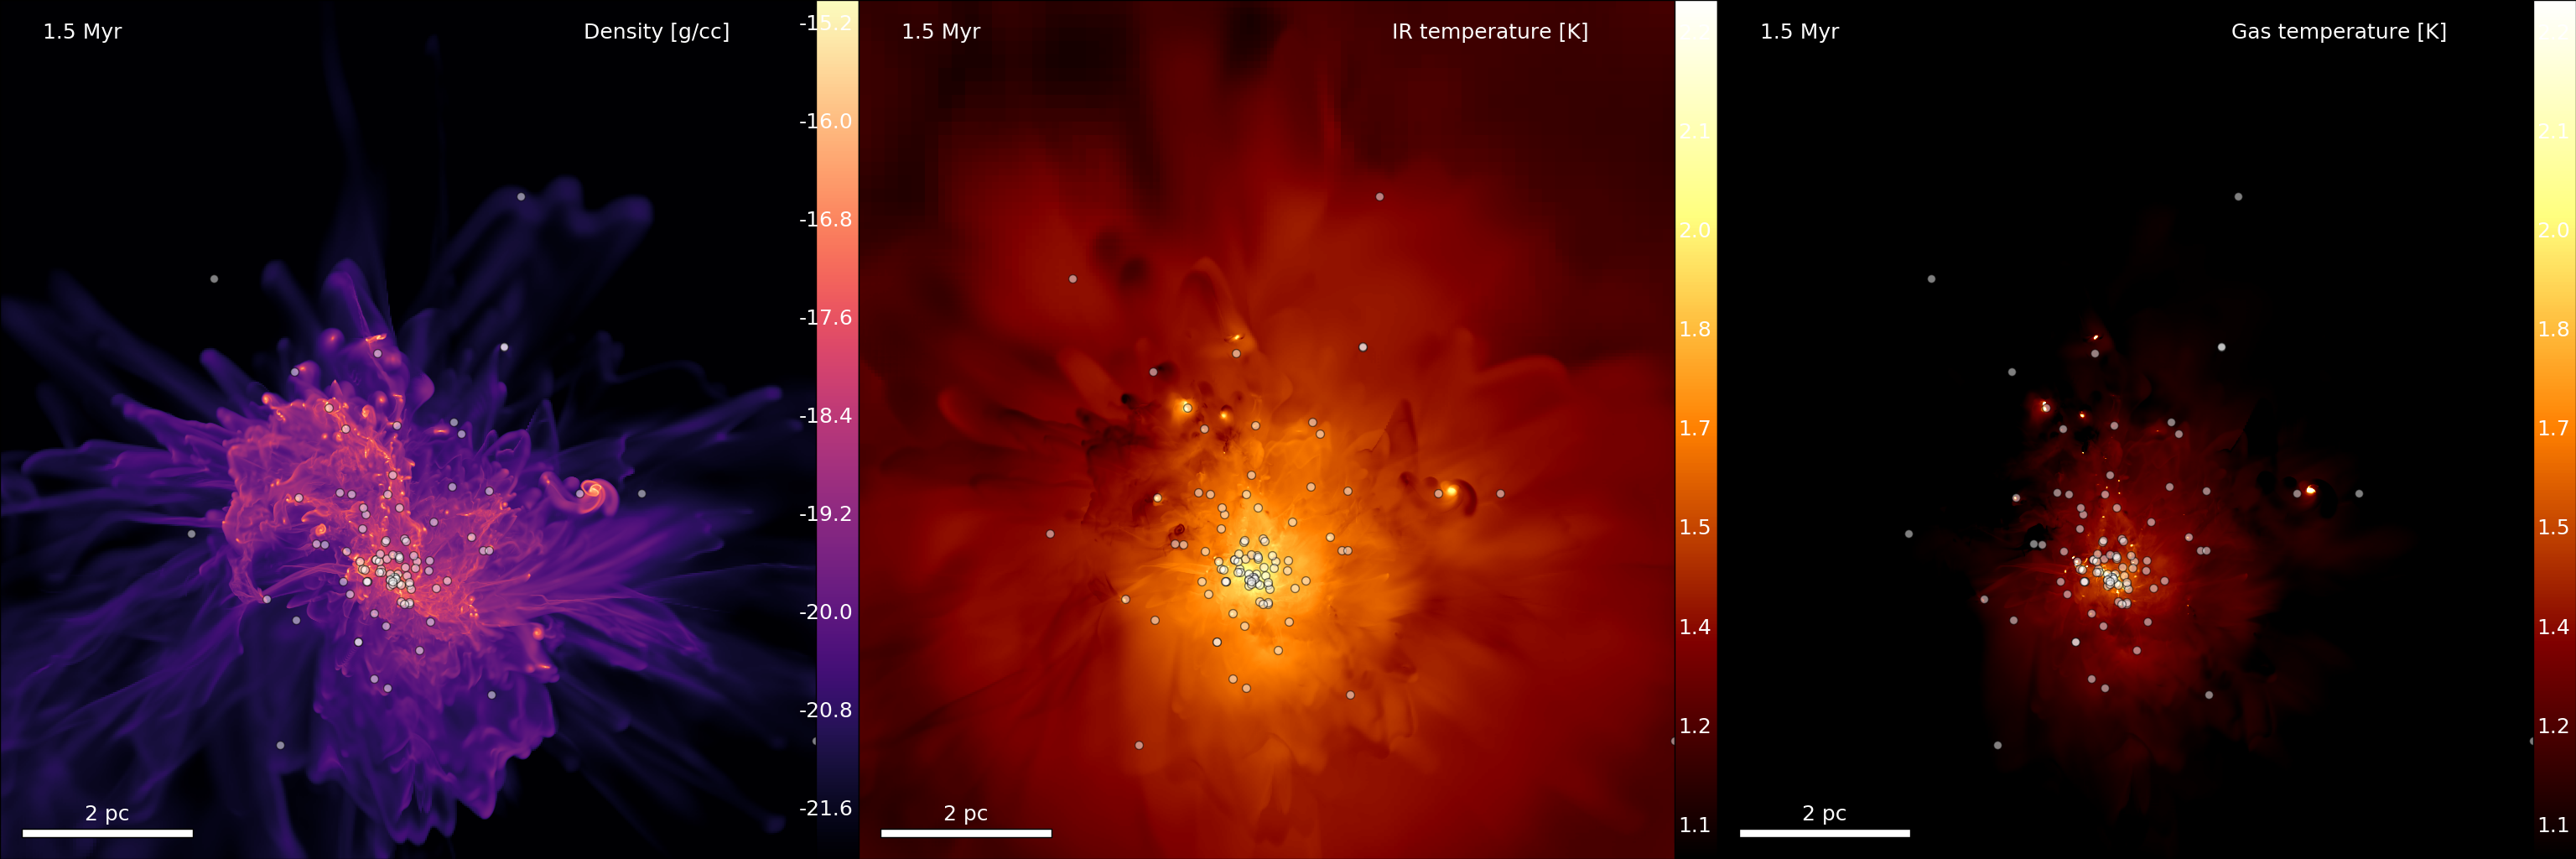
\includegraphics[width=1.05\textwidth]{Figures/cloud_snapshots/multi_00800}
 \captionsetup{justification=justified,singlelinecheck=false,width=\linewidth}
 \decoRule
 \caption[Molecular cloud simulation snapshots]{Snapshots of the molecular cloud's density, radiation and gas temperature.}
 \label{fig:CloudPt3}
\end{figure*}
\FloatBarrier


% Eddington ratio----------------------------------------------------------------------------------------
\subsection{Eddington analysis}
\label{subsec:Eddington_ratio}

\citet{Skinner_Ostriker} used in the analysis of their simulated cloud the Eddington ratio to quantify how strong radiation opposes gravity.
To follow their example we introduce the Eddington ratio

\begin{equation}
  f_{Edd}(r) = \frac{\kappa\rho F_{rad}}{c \rho g}
\label{eq:Eddington_ratio}
\end{equation}

where $\kappa$ is the frequency--averaged opacity, $F_{rad}$ the total radiation flux, and $g$ the gravitational acceleration towards the center.
It represents the fraction between radiational and gravitational force~\footnote{in this form, it actually describes a ratio of \textit{force densities}} exerted on the gas in the cloud.
Are the two forces in equilibrium the Eddington ratio is 1.
A value of the Eddington ratio $< 1$ indicates that the gas in the cloud feels a net inward force and vice versa.

In the simulation, sink particles act as radiation sources as a resulting effect of the mass accretion.
Therefore their luminosity $L_{rad}$ can be used as approximation for the radiation flux

\begin{equation}
  F_{rad} = \frac{L_{rad}}{4\pi r^{2}}
\end{equation}

This approximation unfortunately only holds further away from the sink in the optically thin regime.
For the optically thick regime, the diffusion limit has to be taken into account; see in \secref{subsec:Diffusion_limit}.

The diffusive limit with the assumption that gas and radiation are roughly in thermal equilibrium, fixes the flux in the optically thick regime.

\begin{equation}
  F_{rad} \simeq -\frac{c\lambda_{R}}{3} \nabla E \simeq - \frac{4ca}{3\kappa\rho} T^{3} \nabla T
\end{equation}

where $a$ is the radiation constant and $T$ the temperature of the gas.

The Eddington ratio as described by \eqnref{eq:Eddington_ratio} indicates the net force of two opposing forces, namely radiation and gravity.
Thereby, other influences have been neglected such as gas pressure gradients or centrifugal forces.

\begin{equation}
  \rho \frac{GM}{r^{2}} = \frac{4}{3}a T^{3}\nabla T + \rho \frac{k_{B} \nabla T}{\mu m_{H}} + \rho \frac{v_{\theta}^{2}}{r}
\end{equation}

Here, the left hand side describes the strong gravitational term, on the right hand side we have the radiation term, the gas pressure term, and the centrifugal term (in order).
Due to the temperature's high exponent in the radiation force term, radiation pressure gradients dominate over all other forces already at around 200 K for a gas at $10^{-15}$ g/cc.

This means that other force contribution might still play a role on the outskirts of the cloud, where the temperature is still very close to the modeled ISM temperature, but towards the center the radiation pressure dominates.

Figures~\ref{fig:Cloud_density}, \ref{fig:Cloud_temperature} and \ref{fig:Cloud_tau} show profiles of the cloud at a late time in the simulation.
At that time, already almost hundred sinks have formed and removed a considerable amount of gas mass from the cloud.
The center part of the cloud moved from an optically thin regime to a optical depth well beyond 1.
With the rise in sink number more and more radiation sources appeared.
The radiation emitted by them got trapped by the optically thick gas and heated the gas to the order of $\sim10^{2}$ K.

In combining these profiles according to \eqnref{eq:Eddington_ratio}, the Eddington ratio profile can be calculated; see \figref{fig:Cloud_eddington}.
It shows two Eddington ratio profiles, one with the flux approximated with the diffusion limit, the other with an optically thin flux approximation.
Their lines almost perfectly match, where the optical depth crosses the value 1.
The curves in their valid regimes are almost consistently below the Eddington limit, which indicates that a majority of the gas in the cloud still feels a net inward force.
This also agrees well with the findings of \citet{Skinner_Ostriker}.
However, the temperature of the cloud only started to rise towards $10^{2}$ K, which means other forces might still have some considerable influence on the gas.

\begin{figure}[!htb]
 \centering
 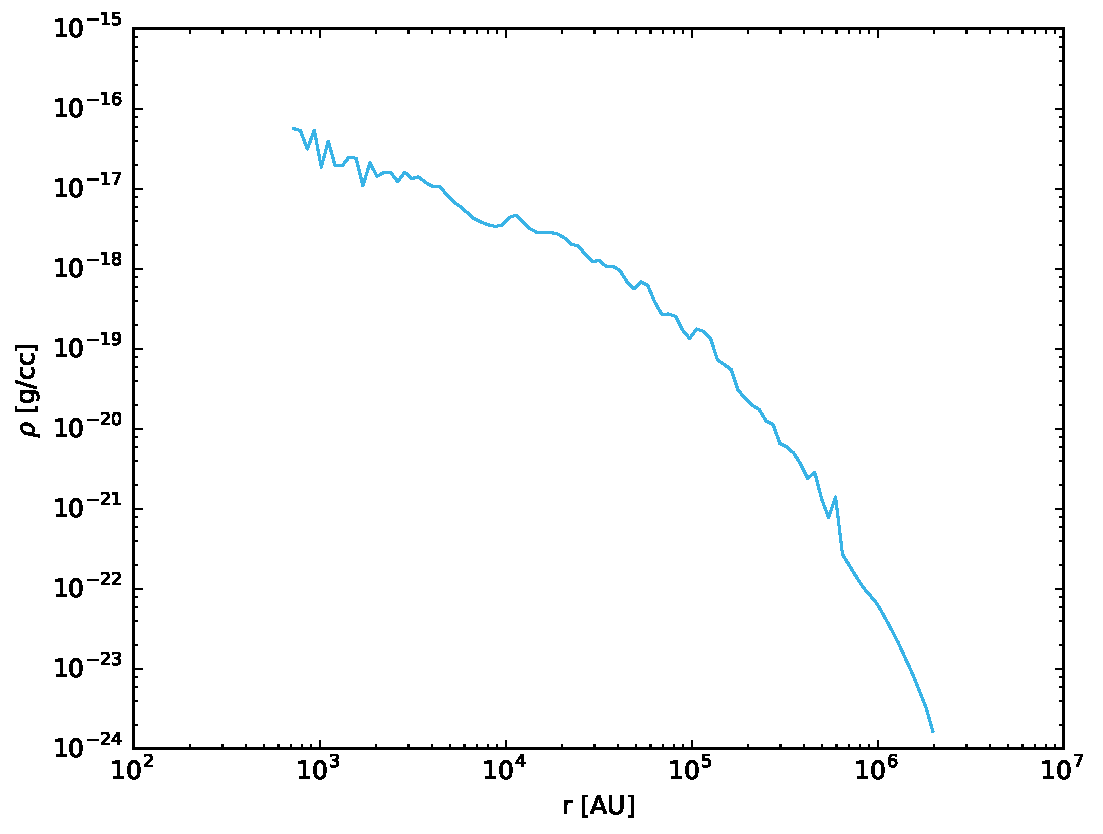
\includegraphics[width=0.9\textwidth]{Figures/cloud_profiles/density_profile}
 \captionsetup{justification=justified,singlelinecheck=false,width=\linewidth}
 \decoRule
 \caption[Cloud density profile]{The simulated cloud's density profile at a simulated time of 1.3724 Myrs.
                                 It includes the entire cloud's gas mass, but omits sink particle masses.}
 \label{fig:Cloud_density}
\end{figure}

\FloatBarrier

\begin{figure}[!htb]
 \centering
 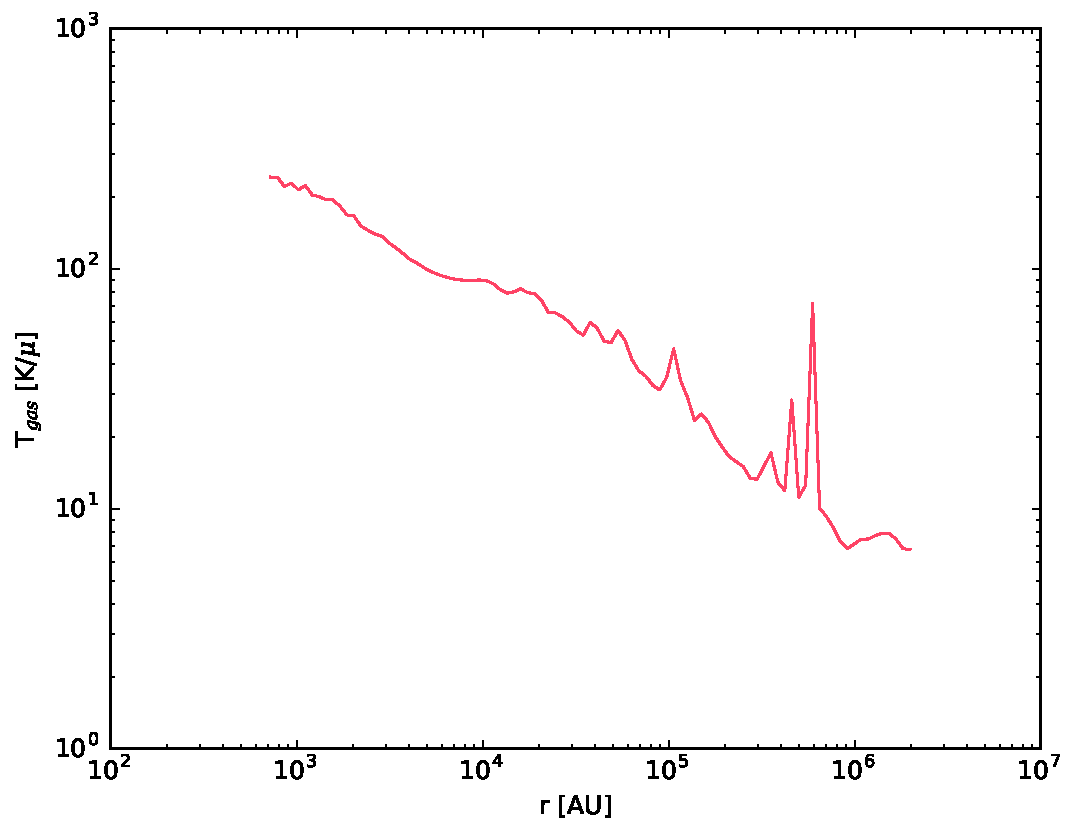
\includegraphics[width=0.9\textwidth]{Figures/cloud_profiles/temp_profile}
 \captionsetup{justification=justified,singlelinecheck=false,width=\linewidth}
 \decoRule
 \caption[Cloud temperature profile]{The simulated cloud's temperature profile at a simulated time of 1.3724 Myrs.
                                     Radiation emitted from sinks in the center of the cloud heat up the gas to almost 200 K.
                                     The peaks at $5\cdot10^{5}$ and $7\cdot10^{5}$ AU are due to very massive sinks with high luminosities heating the gas in their proximity.}
 \label{fig:Cloud_temperature}
\end{figure}

\FloatBarrier

\begin{figure}[!htb]
 \centering
 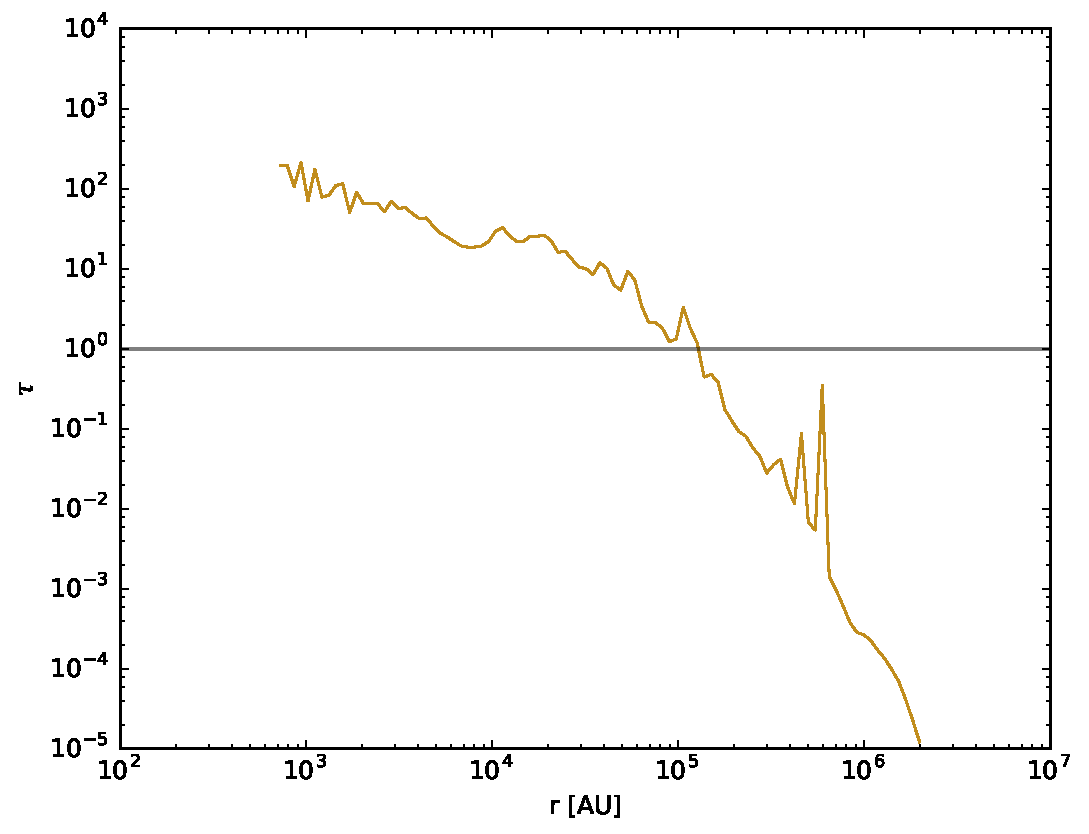
\includegraphics[width=0.9\textwidth]{Figures/cloud_profiles/tau_profile}
 \captionsetup{justification=justified,singlelinecheck=false,width=\linewidth}
 \decoRule
 \caption[Cloud's optical depth profile]{The simulated cloud's optical depth profile at a simulated time of 1.3724 Myrs.
                                         It is calculated according to \eqnref{eq:Skinner_Ostriker_RSLA}, with an opacity profile $\kappa\propto T^{2}$ according to \citet{Davisetal}.}
 \label{fig:Cloud_tau}
\end{figure}

\FloatBarrier

\begin{figure}[!htb]
 \centering
 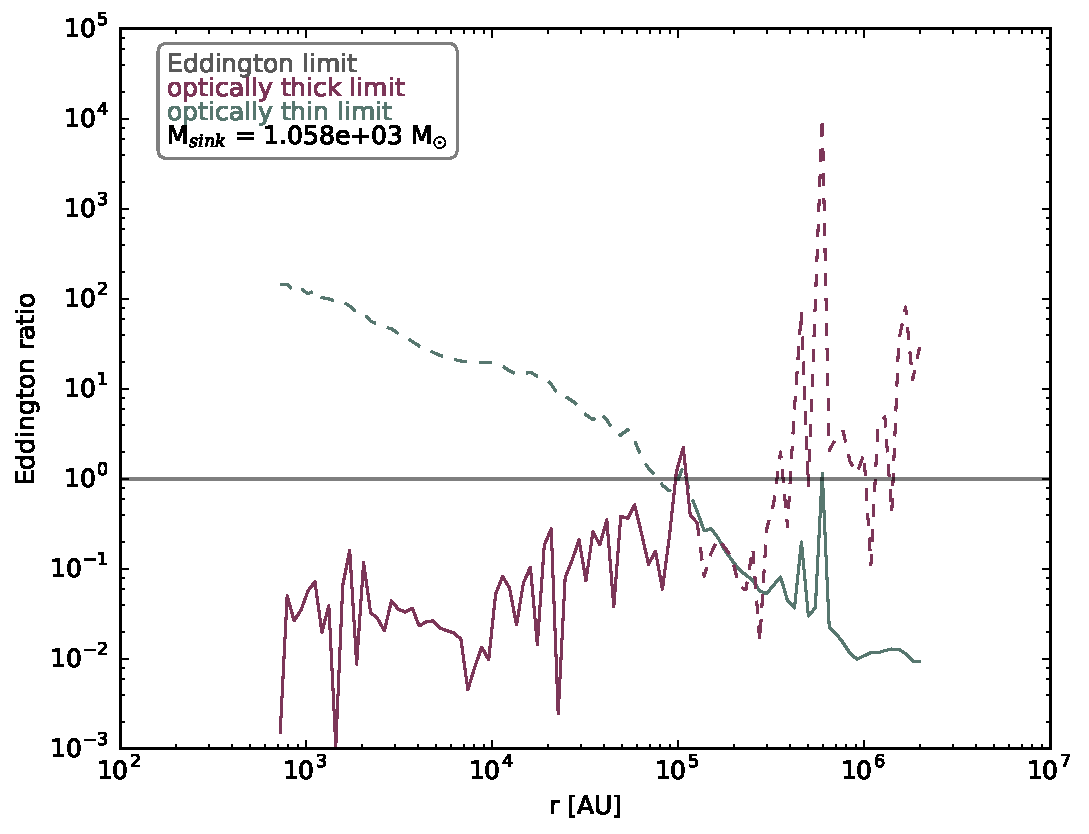
\includegraphics[width=0.9\textwidth]{Figures/cloud_profiles/eddington_limits}
 \captionsetup{justification=justified,singlelinecheck=false,width=\linewidth}
 \decoRule
 \caption[Cloud's Eddington ratio profile]{The simulated cloud's Eddington ratio profile at a simulated time of 1.3724 Myrs.
                                           Throughout the cloud the Eddington ratio lies below 1, indicating that a majority of the gas mass still feels the gravitational pull towards the center.}
 \label{fig:Cloud_eddington}
\end{figure}
\FloatBarrier


% Star cluster----------------------------------------------------------------------------------------
\subsection{Star cluster}
\label{subsec:Star_cluster}

The analysis of the star cluster in the center of the cloud reveals interesting circumstances.
At the end of the simulation, roughly half of the cloud's gas mass has been converted into sink particles.
The mass range of these particles goes from $\sim0.1$ M$_{\odot}$ up to $\sim1000$ M$_{\odot}$.
This range unfortunately does not conform with the initial stellar mass function described by \citet{Charbier, Kroupa}.
In the last snapshot of \figref{fig:CloudPt3} the most massive sink in the simulation can be seen leaving the cloud on the upper right.

The escape of the most massive sink from the cluster has grave consequences.
It throws the cluster off balance and de--virializes the system.
To understand the virialization of clusters, we introduce the virial parameter

\begin{equation}
  \alpha = \frac{2 E_{kin}}{E_{pot}} \sim \frac{2\cdot(1/2)M\sigma^{2}}{(3/5)GM^{2}R^{-1}} = \frac{5\sigma^{2}R}{3GM}
\end{equation}

where $\sigma$ is the cluster's velocity dispersion, $M$ the collective sink mass and $R$ the cluster's radius.

\figref{fig:Cluster_virial} presents the virial analysis of the simulation's cluster.
It shows what already was mentioned above.
The first panel describes the virial parameter of the cluster during the most critical time in the simulation.
At around 1 Myr a jump appears in the evolution of the virial parameter and disrupts the the cluster's equilibration.
This can be accredited to the escape of a massive sink, in fact the most massive in the simulation.
By leaving the cluster, it removes a considerable fraction of mass from the cluster.
Therefore, the virial parameter increases.
After a while the cluster tends to virialize again.
It is barely visible in the plot, however in the end of the simulation two medium sized sinks escape the cluster again which would increase the virial parameter again.
The second panel shows the rate with which the the gas is converted into sinks.
The rate is kept relatively steady and agrees well with the third panel.
It describes the similarly steady rate with which the sink particle number increases, or in a few cases decreases in which the sink particles merge.

The cloud simulation also shows some interesting differences to the reference run of the cloud with an polytropic EOS, we performed.
The pure--hydrodynamics reference run displays much higher sink numbers; see \figref{fig:Cluster_HDvirial}.
Gas to sink mass conversion percentages and relative sink count of the reference run are much higher in comparison, and the average sink mass is smaller by almost a factor of 6.
This also agrees with the findings of the idealized core collapses, where it was found that sink masses are much higher when radiation is included.
There the radiation slows down the collapse by heating the center region and thus supports the resulting disks, which enables the sinks to slowly form, accrete mass with a steady rate and consequently grow to a higher mass.
In the reference runs without radiation, the collapse is much faster, leading to fragmentation and therefore smaller sink masses.
Contrary to the reference run which shows no tendency to virialize, the star cluster of the RT--simulation tends to equilibrate.
It seems that the collapse of the cloud is 'quieter' and slower when radiation is involved, which enables the resulting star cluster to possibly equilibrate.
However, without radiation the collapse is much too fast and violent, which causes the emerging star cluster to explode.
This can also be seen in the beginning in the first panels of both figures.
Within 0.4 Myrs the star cluster from the reference run already reached the virial equilibrium line, whereas the star cluster with radiation
Nevertheless, based on the virial parameters at the end of both simulations alone, both clusters have very similar virial parameters and should disperse.

The heating effect might also be the explanation for another curiosity.
In the reference simulation were much fewer binary and no ternary systems at all.
Higher temperatures help in the stabilization and virialization of multi--body systems.

Unfortunately, it is not clear how much influence the radiation force has on the star clusters, since we simply have not enough data to draw supported conclusions.

\begin{figure}[!htb]
 \centering
 \includegraphics[width=0.9\textwidth]{Figures/cloud_plots/virial_IRcloud}
 \captionsetup{justification=justified,singlelinecheck=false,width=\linewidth}
 \decoRule
 \caption[The star cluster's virial analysis]{The virial analysis of the simulated cloud's star cluster.
                                              The first panel shows the evolution of the virial parameter during the whole simulation.
                                              Panel 2 displays the relative sink to gas mass fraction.
                                              Panel 3 displays the difference of sink count at a particular time step and at the previous time step.
                                              The forth panel shows the average sink mass at a particular time in the simulation.}
 \label{fig:Cluster_virial}
 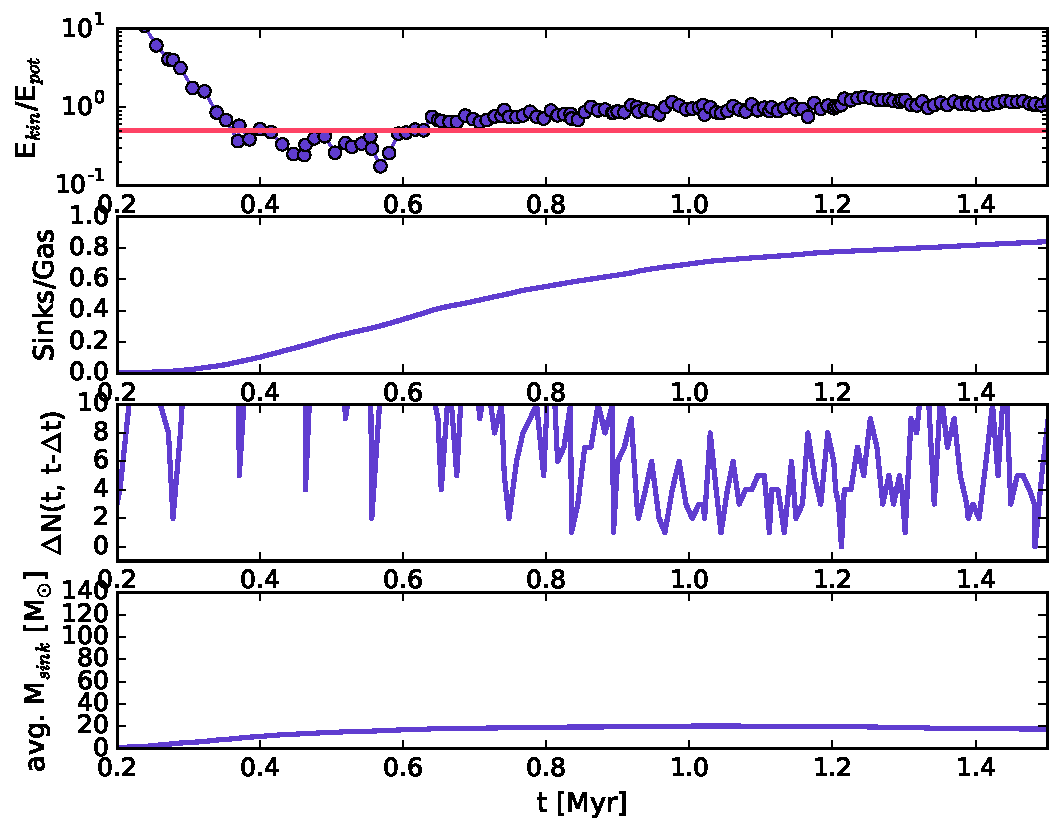
\includegraphics[width=0.9\textwidth]{Figures/cloud_plots/virial_noRTcloud}
 \captionsetup{justification=justified,singlelinecheck=false,width=\linewidth}
 \decoRule
 \caption[Reference run's virial analysis]{The virial analysis of the simulated cloud's star cluster in the reference run.
                                           In comparison with \figref{fig:Cluster_virial} we can see that at around 1.4 Myrs the reference run has already converted 80\% of all the present gas into sinks, while the RT--simulation has converted only 50\%.
                                           The overall sink formation rate also seems to be much higher.
                                           However, the average sink mass is lower in the reference run by almost a factor of 6.}
 \label{fig:Cluster_HDvirial}
\end{figure}
\FloatBarrier


%\newpage
% Conclusion ----------------------------------------------------------------------------------------
\section{Conclusion}
\label{sec:Conclusion}

% %TODO Conclusion chapter

In this thesis, radiation hydrodynamics simulations of sphere collapses and ultimately of a molecular cloud were presented.

After an introduction to the morphology of molecular clouds, the birth places of stars and star formation in general, the radiation hydrodynamics theory was construed.
The importance of the radiation's influence on star formation has been acknowledged by the astrophysics community since long and computer simulations gradually became efficient enough to numerically model radiation hydrodynamics directly.

To that end, in a subsequent chapter some numerical methods were described, which help implementing the radiation hydrodynamics theory into astrophysical simulation tools.
With the introduction of such a program, called RAMSES, which was used to perform the simulations in this thesis, the chapter was finished.
\\[6pt]
%
Here, in the last chapter, details to the different kinds of performed simulations were explained.

\begin{itemize}
  \item First, pure--hydrodynamics of core collapses were tested without radiation.
        Excessive fragmentation and a high number of low--mass sinks were typical outcomes of these simulations.
        However, this behavior was expected.
        They were intended to serve as reference for following tests to compare to and improve on.
  \item The second phase of runs involved and focused on the radiative transfer module of RAMSES, and in particular two parameters whose purpose were to optimize the numerical scheme.
        These parameters control the update of the reduced speed of light approximation and subcycling of the thermochemistry step, which calculates the effect of the (infrared) radiation onto matter.
        Although the computing times were almost doubled compared to the reference runs, an improvement concerning fragmentation could be observed.
        Around the sinks which act as radiation sources, the gas appeared much more diffuse due to the heat transfered by the infrared radiation.
        However, this effect is at most mid--ranged and fragmentation was not stopped in the outskirts of the spheres.
        The routines calculating the updates for the reduced speed of light approximation were deemed ineffective and not worth the computational resources.
  \item Subsequently, the disk stability of initially rotating singular isothermal sphere profiles was investigated with pure--hydrodynamics as well as radiative transfer simulations.
        Several variants of singular isothermal spheres were used as initial conditions with different masses and resolutions.
        Ulterior motives of these tests were to prepare to move to entire molecular clouds with a mass of the order of $\sim10^{4}$ M$_{\odot}$.
        The Toomre parameter analysis showed that disks are more stable when their gas is heated by the radiation.
        When the gas stays at 10 K, fragmentation causes disk instabilities.
  \item Finally, an entire molecular cloud with a mass of around $2.3\cdot10^{4}$ M$_{\odot}$ was simulated.
        Only a single photon group in the infrared spectrum was employed to investigate its isolated behavior.
        In the investigation of the radiation force from the most massive sink inside the cloud, it was concluded that even though the effect is slight, the force from radiation is able to withstand gravity to some degree.
        In comparison to the reference run of the same cloud, the sink particle number appeared to be considerably lower after $1.4$ Myrs, while the sink masses were much higher.
        It could be concluded that the infrared radiation effectively delays sink particle formation by heating the cloud's gas.
        The rise in gas temperature due to infrared radiation also must have affected the dynamics of the sink systems.
        Contrary to reference runs, several stable ternary systems were observed.
\end{itemize}

These simulations alone unfortunately are not enough to explain the low observed star formation efficiencies in our and nearby galaxies.
However, combined with higher energy photons in the ultraviolet spectrum from more massive stars, simulated star formation efficiencies could already approach the observed numbers.
Nevertheless, radiation definitely improves our understanding of star formation.
In the future, radiative transfer routines will definitely be improved through either utilization of GPUs or improvements in numerical schemes such as faster implicit time stepping methods.
It might even not be long until simulations involving radiation hydrodynamics and magnetohydrodynamics can be efficiently performed to gain even deeper understanding in star formation.

%\include{Chapters/Chapter5}

%----------------------------------------------------------------------------------------
%	THESIS CONTENT - APPENDICES
%----------------------------------------------------------------------------------------

\appendix % Cue to tell LaTeX that the following "chapters" are Appendices

% Include the appendices of the thesis as separate files from the Appendices folder

% Uncomment the lines as you write the Appendices

% !TEX root = ../main.tex
% Appendix A

\chapter{Derivation of the Euler equations} % Main appendix title

\label{AppendixA} % For referencing this appendix elsewhere, use \ref{AppendixA}

The Euler equations Eqs.~\eqref{eq:EulerMass}, \eqref{eq:EulerMomentum}, and \eqref{eq:EulerEnergy} are derived by taking moments, i.e., $m\cdot\int_{\mathbb{R}^{3}} \mathrm{d}^{3}v$, $m\cdot\int_{\mathbb{R}^{3}}\,\textbf{v}\,\mathrm{d}^{3}v$ and $m\cdot\int_{\mathbb{R}^{3}}\,\frac{v^{2}}{2}\,\mathrm{d}^{3}v$, of the Boltzmann equation \eqref{eq:BoltzmannEQ}.

\begin{equation*}
  \frac{\partial f}{\partial t} + \dot{\textbf{x}} \frac{\partial f}{\partial \textbf{x}} + \dot{\textbf{v}} \frac{\partial f}{\partial \textbf{v}} = \Big(\frac{Df}{Dt}\Big)_{\text{coll.}}
\end{equation*}

Since these moments represent collisional invariants, the collision integral is averaged to zero (see \secref{sec:HydrodynamicEquations}).
\begin{itemize}
 \item The first moment ($m\cdot\int \mathrm{d}^{3}v$) of the Boltzmann equation reads
 \begin{align*}
  &0 = m \int\,\frac{\partial f}{\partial t}\,\mathrm{d}^{3}v \,+\, m \int\,\dot{\textbf{x}}\,\frac{\partial f}{\partial \textbf{x}}\,\mathrm{d}^{3}v \,+\, m \int\,\dot{\textbf{v}}\,\frac{\partial f}{\partial \textbf{v}}\,\mathrm{d}^{3}v \\
  \Longleftrightarrow\qquad
  &0 = \frac{\partial}{\partial t} \underbrace{ \int\,m  f\,\mathrm{d}^{3}v }_{\rho(\textbf{x}, t)} \,+\, \underbrace{ \frac{\partial}{\partial \textbf{x}} }_{\nabla} \int\,m \underbrace{ \dot{\textbf{x}} }_{\textbf{v}} f\,\mathrm{d}^{3}v \,+\, m \int\,\underbrace{ \dot{\textbf{v}} }_{\textbf{a}} \frac{\partial f}{\partial \textbf{v}}\,\mathrm{d}^{3}v \\
  \Longleftrightarrow\qquad
  &0 = \frac{\partial}{\partial t} \rho(\textbf{x}, t) \,+\, \nabla \underbrace{ \int\,m \textbf{v} f\,\mathrm{d}^{3}v }_{\rho(\textbf{x}, t)  \textbf{u}} \enskip+\enskip m\,\textbf{a} \underbrace{ \int\,\frac{\partial f}{\partial \textbf{v}}\,\mathrm{d}^{3}v }_{ \mathclap{[f(\infty) - f(-\infty)] \rightarrow 0} }
 \end{align*}
 In the first step, we have used the Leibniz integral rule, whereas in the second step we have used the moments of the distribution function itself, see Eqs.~\eqref{eq:fmoment1} and \eqref{eq:fmoment2}.
 Since $f$ is a well--behaved distribution function, it has the property: $f \rightarrow 0$ for $\textbf{v} \rightarrow \pm \infty$, from which follows $[f(\textbf{v} = \infty) - f(\textbf{v} = -\infty)] \rightarrow 0$.
 This yields the first Euler equation \eqref{eq:EulerMass}, representing the conservation of mass.
 \begin{align*}
  \Aboxed{\frac{\partial\rho}{\partial t} \,+\, \nabla(\rho\textbf{u}) = 0}
 \end{align*}

 \item The second moment ($m \int\,\textbf{v}\,\mathrm{d}^{3}v$) of the Boltzmann equation reads
 \begin{align*}
  &0 = m \int\,\textbf{v}\frac{\partial f}{\partial t}\,\mathrm{d}^{3}v \,+\, m \int\,\textbf{v}\,\dot{\textbf{x}}\,\frac{\partial f}{\partial \textbf{x}}\,\mathrm{d}^{3}v \,+\, m \int\,\textbf{v}\,\dot{\textbf{v}}\,\frac{\partial f}{\partial \textbf{v}}\,\mathrm{d}^{3}v \\
  \Longleftrightarrow\qquad
  &0 = \frac{\partial}{\partial t} \underbrace{ \int\,m \textbf{v}f\,\mathrm{d}^{3}v }_{\rho(\textbf{x}, t)\textbf{u}} \,+\, \underbrace{ \frac{\partial}{\partial \textbf{x}} }_{\nabla} \int\,m \underbrace{ \textbf{v}\,\dot{\textbf{x}} }_{\textbf{v}\otimes\textbf{v}} f\,\mathrm{d}^{3}v \,+\, m \int\,\textbf{v}\,\underbrace{ \dot{\textbf{v}} }_{\textbf{a}} \frac{\partial f}{\partial \textbf{v}}\,\mathrm{d}^{3}v \\
  \Longleftrightarrow\qquad
  &0 = \frac{\partial(\rho \textbf{u})}{\partial t} \,+\, \nabla \int\,m \big(\textbf{v}\otimes\textbf{v}\big) f\,\mathrm{d}^{3}v \,+\, m \textbf{a}\,\underbrace{ \int\,\textbf{v}\,\frac{\partial f}{\partial \textbf{v}}\,\mathrm{d}^{3}v }_{\mathclap{\int\,\alpha\beta'\,\mathrm{d}s = \alpha\beta\mid_{-\infty}^{\infty} - \int\,\alpha'\beta\,\mathrm{d}s}}
 \end{align*}
 Again, we have used the Leibniz integral rule and the definitions of the distribution function's moments.
 Here, the second term can be written with $\textbf{v} = \textbf{u} + \textbf{w}$, where $\textbf{w}$ describes the thermal velocity with an average of $\langle \textbf{w}\rangle = 0$, such that the average fluid velocity still remains $\langle \textbf{v}\rangle = \textbf{u}$.
 Using integration by parts on the third term with $\alpha = \textbf{v}$, $\alpha' = 1$, $\beta' = \frac{\partial f}{\partial\textbf{v}}$, and $\beta = f$, we get
 \begin{align*}
 \Longleftrightarrow\qquad
  &0 = \frac{\partial(\rho \textbf{u})}{\partial t} \,+\, \nabla \int\,m \big(\textbf{v}\otimes\textbf{v}\big) f\,\mathrm{d}^{3}v \,+\, m \textbf{a}\,\big(\underbrace{ \textbf{v}\,f\mid_{-\infty}^{\infty} }_{\mathclap{f \rightarrow 0 \text{ for } \textbf{v} \rightarrow \pm \infty}} - \underbrace{ \int\,f\mathrm{d}^{3}v }_{n(\textbf{x}, t)}\big)
 \end{align*}
 where $n(\textbf{x}, t) = \frac{\rho(\textbf{x}, t)}{m}$ is the number density.
 Again, the distribution function is well--behaved, which is why the first term in the parenthesis goes to zero.
 From this point on, the second term is easier to understand if we make use of Einstein's notation
 \begin{align*}
 \Longleftrightarrow\qquad
  &0 = \frac{\partial(\rho u_{i})}{\partial t} \,+\, \nabla \int\,m \,\underbrace{ \big(v_{i}v_{j}\big) }_{\mathclap{u_{i}u_{j} + w_{i}w_{j} + u_{i}w_{j} + u_{j}w_{i}}} f\,\mathrm{d}^{3}v \,-\, \rho\,a_{i} \\
  \Longleftrightarrow\qquad
  &0 = \frac{\partial(\rho u_{i})}{\partial t} \,+\, \nabla \int\,m \,\big(u_{i}u_{j} + w_{i}w_{j} + u_{i}w_{j} + u_{j}w_{i}\big) f\,\mathrm{d}^{3}v \,-\, \rho\,a_{i} \\
  \Longleftrightarrow\qquad
  &0 = \frac{\partial(\rho u_{i})}{\partial t} \,+\, \nabla m \,\big( \int u_{i}u_{j} f\,\mathrm{d}^{3}v + \int w_{i}w_{j} f\,\mathrm{d}^{3}v \\
   &\hspace{76pt} + \int u_{i}w_{j} f\,\mathrm{d}^{3}v + \int u_{j}w_{i} f\,\mathrm{d}^{3}v\big) \,-\, \rho\,a_{i} \\
  \Longleftrightarrow\qquad
  &0 = \frac{\partial(\rho u_{i})}{\partial t} \,+\, \nabla m \,\big( \int u_{i}u_{j} f\,\mathrm{d}^{3}v + \int w_{i}w_{j} f\,\mathrm{d}^{3}v \\
   &\hspace{66pt} + u_{i} \underbrace{ \int w_{j} f\,\underbrace{ \mathrm{d}^{3}v }_{\mathrm{d}^{3}w} }_{n(\textbf{x}, t)\langle \textbf{w}\rangle = 0} \,+\, u_{j} \underbrace{ \int w_{i} f\,\underbrace{ \mathrm{d}^{3}v }_{\mathrm{d}^{3}w} }_{n(\textbf{x}, t)\langle \textbf{w}\rangle = 0}\big) \,-\, \rho\,a_{i} \\
  \Longleftrightarrow\qquad
  &0 = \frac{\partial(\rho u_{i})}{\partial t} \,+\, \nabla m \,\big( \underbrace{ \int u_{i}u_{j} f\,\mathrm{d}^{3}v }_{(u_{i}u_{j})n(\textbf{x}, t)} + \int w_{i}w_{j} f\,\mathrm{d}^{3}v\big) \,-\, \rho\,a_{i} \\
  \Longleftrightarrow\qquad
  &0 = \frac{\partial(\rho u_{i})}{\partial t} \,+\, \nabla \big( \rho(u_{i}u_{j}) + \underbrace{ \int m  w_{i}w_{j} f\,\mathrm{d}^{3}v}_{\equiv \mathbb{P}_{ij}} \big) \,-\, \rho\,a_{i}
 \end{align*}
 In the last step, we used the definition for the pressure tensor $\mathbb{P}_{ij} \equiv \int m  w_{i}w_{j} f\,\mathrm{d}^{3}w$.
 Rewriting this final equation again in vectorial form, recovers the second Euler equation \eqref{eq:EulerMomentum}.
 \begin{align*}
  \Aboxed{\frac{\partial(\rho \textbf{u})}{\partial t} \,+\, \nabla \big( \rho(\textbf{u}\otimes\textbf{u}) + \mathbb{P} \big) = \rho\,\textbf{a}}
 \end{align*}

 \item The third moment ($m \int_{\mathbb{R}^{3}}\,\frac{v^{2}}{2}\,\mathrm{d}^{3}v$) of the Boltzmann equation reads
 \begin{align*}
  &0 = m \int\,\underbrace{ \frac{v^{2}}{2} }_{\mathclap{\frac{u^{2}}{2}+\frac{w^{2}}{2}+\textbf{u}\cdot\textbf{w}}}\frac{\partial f}{\partial t}\,\mathrm{d}^{3}v \,+\, m \int\,\underbrace{ \frac{v^{2}}{2} }_{\mathclap{\frac{u^{2}}{2}+\frac{w^{2}}{2}+\textbf{u}\cdot\textbf{w}}}\,\underbrace{ \dot{\textbf{x}} }_{\textbf{v}}\,\frac{\partial f}{\partial \textbf{x}}\,\mathrm{d}^{3}v \,+\, m \int\,\frac{v^{2}}{2}\,\underbrace{ \dot{\textbf{v}} }_{\textbf{a}}\,\frac{\partial f}{\partial \textbf{v}}\,\mathrm{d}^{3}v \\
  \Longleftrightarrow\qquad
  &0 = \frac{\partial}{\partial t}\Big( \int m \frac{u^{2}}{2}f\,\mathrm{d}^{3}v + \underbrace{ \int\,m \frac{w^{2}}{2}f\,\underbrace{ \mathrm{d}^{3}v }_{\mathrm{d}^{3}w} }_{\mathclap{\equiv\,\rho\epsilon}} + m\,\textbf{u}\underbrace{ \int m\,\textbf{w}\,f\,\underbrace{ \mathrm{d}^{3}v }_{\mathrm{d}^{3}w} }_{n(\textbf{x}, t)\langle \textbf{w}\rangle = 0} \Big) \\
   &\hspace{3pt} +\, \underbrace{ \frac{\partial}{\partial\textbf{x}} }_{\nabla}\Big( \int m\,\frac{u^{2}}{2}\textbf{v}\,f\,\mathrm{d}^{3}v + \int\,m\,\frac{w^{2}}{2}\textbf{v}\,f\,\mathrm{d}^{3}v + \int\,m\,\big(\textbf{u}\cdot\textbf{w}\big)\textbf{v} f\,\mathrm{d}^{3}v \Big) \\
   &\hspace{3pt} +\, m\,\textbf{a} \underbrace{\int\,\frac{v^{2}}{2}\,\frac{\partial f}{\partial \textbf{v}}\,\mathrm{d}^{3}v }_{\mathclap{\int\,\alpha\beta'\,\mathrm{d}s = \alpha\beta\mid_{-\infty}^{\infty} - \int\,\alpha'\beta\,\mathrm{d}s}}
 \end{align*}
 As in the derivations before, we have made use of the Leibniz integral rule, the thermal velocity $\textbf{w} = \textbf{v} - \textbf{u}$ with $\langle \textbf{w}\rangle = 0$, and the definitions of the distribution function's moments.
 In the third term, we --- again --- integrate by parts, with $\alpha = \frac{v^{2}}{2}$, $\alpha' = \textbf{v}$, $\beta' = \frac{\partial f}{\partial\textbf{v}}$, and $\beta = f$, and subsequently remember that $f \rightarrow 0$ for $\textbf{v} \rightarrow \pm \infty$, since $f$ is a distribution.
 \begin{align*}
  \Longleftrightarrow\qquad
  &0 = \frac{\partial}{\partial t}\Big( \frac{u^{2}}{2}\underbrace{ \int m\,f\,\mathrm{d}^{3}v }_{\rho(\textbf{x}, t)} + \rho\epsilon \Big) \\
   &\hspace{3pt} +\, \nabla\Big( \frac{u^{2}}{2}\underbrace{ \int m\,\textbf{v}\,f\,\mathrm{d}^{3}v }_{\rho(\textbf{x}, t)\textbf{u}} + \int\,m\,\underbrace{ \textbf{v} }_{\mathclap{\textbf{u}+\textbf{w}}} \frac{w^{2}}{2}f\,\mathrm{d}^{3}v + \int\,m\,\big(\textbf{u}\cdot\textbf{w}\big)\underbrace{ \textbf{v} }_{\mathclap{\textbf{u}+\textbf{w}}} f\,\mathrm{d}^{3}v \Big) \\
   &\hspace{3pt} +\, m\,\textbf{a} \big( \underbrace{ \frac{v^{2}}{2}\,f\mid_{-\infty}^{\infty} }_{\mathclap{f \rightarrow 0 \text{ for } \textbf{v} \rightarrow \pm \infty}} - \underbrace{ \int\textbf{v}\,f\,\mathrm{d}^{3}v }_{n(\textbf{x}, t)\textbf{u}} \big) \\
  \Longleftrightarrow\qquad
  &0 = \frac{\partial}{\partial t}\Big( \frac{1}{2}\rho\,u^{2} + \rho\epsilon \Big) \\
   &\hspace{3pt} +\, \nabla\Big( \frac{1}{2}\rho\,u^{2}\,\textbf{u} + \underbrace{ \int\,m\,\big(\textbf{u}+\textbf{w}\big) \frac{w^{2}}{2}f\,\mathrm{d}^{3}v }_{I_{1}} + \underbrace{ \int\,m\,\big(\textbf{u}\cdot\textbf{w}\big)\big(\textbf{u}+\textbf{w}\big) f\,\mathrm{d}^{3}v }_{I_{2}} \Big) \\
   &\hspace{3pt} -\, \rho\,\textbf{a}\,\textbf{u}
 \end{align*}
 For sake of simplicity, we now look at the integrals $I_{1}$ and $I_{2}$ separately. And again, for $I_{2}$ we use Einstein's notation
 \begin{align*}
  I_{1} &= \int m\,\big(\textbf{u}+\textbf{w}\big)\frac{w^{2}}{2}\,f\,\mathrm{d}^{3}v \\
	&= \int m\,\textbf{u}\,\frac{w^{2}}{2}\,f\,\mathrm{d}^{3}v \,+\, \int m\,\textbf{w}\,\frac{w^{2}}{2}\,f\,\mathrm{d}^{3}v \\
	&= \textbf{u}\underbrace{ \int m\,\frac{w^{2}}{2}\,f\,\underbrace{ \mathrm{d}^{3}v }_{\mathclap{\mathrm{d}^{3}w}} }_{\mathclap{\equiv\,\rho\epsilon}} \,+\, \underbrace{ \int m\,\textbf{w}\,\frac{w^{2}}{2}\,f\,\mathrm{d}^{3}v }_{\equiv \textbf{Q}} \\
	&= \rho\epsilon\cdot\textbf{u} + \textbf{Q} \\
  \\
  I_{2} &= \int\,m\,\big(\textbf{u}\cdot\textbf{w}\big)\big(\textbf{u}+\textbf{w}\big) f\,\mathrm{d}^{3}v \\
	&= \int\,m\,\big(\textbf{u}\cdot\textbf{w}\big)\,\textbf{u}\,f\,\mathrm{d}^{3}v \,+\, \int\,m\,\big(\textbf{u}\cdot\textbf{w}\big)\,\textbf{w}\,f\,\mathrm{d}^{3}v \\
	&= \int\,m\,u_{i}\,w_{i}\,u_{j}\,f\,\mathrm{d}^{3}v \,+\, \int\,m\,u_{i}\,w_{i}\,w_{j}\,f\,\mathrm{d}^{3}v \\
	&= u_{i}\,u_{j}\underbrace{ \int\,m\,w_{i}\,f\,\mathrm{d}^{3}v }_{n(\textbf{x}, t)\langle \textbf{w}\rangle = 0} \,+\, \underbrace{ u_{i}\int\,m\,w_{i}\,w_{j}\,f\,\mathrm{d}^{3}v }_{\equiv \mathbb{P}_{ij}\,u_{i}} \\
	&= \mathbb{P}_{ij}\,u_{i} \,=\, \mathbb{P}\,\textbf{u}
 \end{align*}
 Re--substituting both expressions for the integrals $I_{1}$ and $I_{2}$ into the equation before, yields
 \begin{align*}
  &0 = \frac{\partial}{\partial t}\underbrace{ \Big( \frac{1}{2}\rho\,u^{2} + \rho\epsilon \Big) }_{\equiv E} \,+\, \nabla\Big( \underbrace{ \big(\frac{1}{2}\rho\,u^{2} + \rho\epsilon\big) }_{\equiv E} \textbf{u} + \mathbb{P}\,\textbf{u} + \textbf{Q} \Big) \,-\, \rho\,\textbf{a}\,\textbf{u}
 \end{align*}
 The energy density is defined as $E = \frac{1}{2}\rho\,u^{2} + \rho\,\epsilon$ and is the conserved quantity in the third Euler equation \eqref{eq:EulerEnergy} which is the equation above, if one neglects the heat flux term $\textbf{Q}$.
 \begin{align*}
  \Aboxed{\frac{\partial E}{\partial t} \,+\, \nabla\Big(E + \mathbb{P}\Big)\,\textbf{u} = \rho\,\textbf{a}\,\textbf{u}}
 \end{align*}

 \item From this point, knowing that the Lagrangian derivative $\frac{D}{Dt} \equiv \frac{\partial}{\partial t} + \textbf{u} \cdot \nabla$ is also linear, going from Eulerian to Lagrangian form of the equations is not hard.

 \eqref{eq:EulerMass} to \eqref{eq:EulerMassL}:
 \vspace{-0.5cm}
 \begin{align*}
  &\frac{\partial\rho}{\partial t} \,+\, \underbrace{ \nabla(\rho\textbf{u}) }_{\mathclap{\rho\,\nabla\cdot\textbf{u} + \textbf{u}\cdot\nabla\,\rho}} = 0 \\
  \Longleftrightarrow\qquad
  &\underbrace{ \frac{\partial\rho}{\partial t} \,+\, \textbf{u}\cdot\nabla\,\rho }_{\frac{D\rho}{Dt}} \,+\, \rho\,\nabla\cdot\textbf{u} = 0 \\
  \Longleftrightarrow\qquad\!\!
  \Aboxed{&\frac{1}{\rho}\frac{D\rho}{Dt} = -\nabla\cdot\textbf{u}}
 \end{align*}
 \eqref{eq:EulerMomentum} to \eqref{eq:EulerMomentumL}:
 \vspace{-0.5cm}
 \begin{align*}
  &\frac{\partial(\rho \textbf{u})}{\partial t} \,+\, \nabla \big( \rho(\textbf{u}\otimes\textbf{u}) + \mathbb{P} \big) = \rho\,\textbf{a} \\
  \Longleftrightarrow\qquad
  &\textbf{u}\frac{\partial\rho}{\partial t} + \rho\frac{\partial\textbf{u}}{\partial t} \,+\, \underbrace{ \nabla\big(\rho(\textbf{u}\otimes\textbf{u})\big) }_{\mathclap{\rho\big(\textbf{u}(\nabla\cdot\textbf{u}) + (\textbf{u}\cdot\nabla)\textbf{u}\big) + \textbf{u}\big(\textbf{u}\cdot\nabla\,\rho\big)}} = -\nabla\mathbb{P} + \rho\,\textbf{a} \\
  \Longleftrightarrow\qquad
  &\underbrace{ \textbf{u}\frac{\partial\rho}{\partial t} + \textbf{u}\big(\textbf{u}\cdot\nabla\,\rho\big) }_{\mathclap{\textbf{u}\frac{D\rho}{Dt} = \,-\rho\textbf{u}\big(\nabla\cdot\textbf{u}\big)}} \,+\, \underbrace{ \rho\frac{\partial\textbf{u}}{\partial t} + \rho(\textbf{u}\cdot\nabla)\textbf{u} }_{\mathclap{\rho\frac{D\textbf{u}}{Dt}}} \,+\, \rho\textbf{u}(\nabla\cdot\textbf{u}) = -\nabla\mathbb{P} + \rho\,\textbf{a} \\
  \Longleftrightarrow\qquad
  &\rho\frac{D\textbf{u}}{Dt} \,-\, \rho\textbf{u}\big(\nabla\cdot\textbf{u}\big) \,+\, \rho\textbf{u}(\nabla\cdot\textbf{u}) = -\nabla\mathbb{P} + \rho\,\textbf{a} \\
  \Longleftrightarrow\qquad\!\!
  \Aboxed{&\rho\frac{D\textbf{u}}{Dt} = -\nabla\mathbb{P} + \rho\,\textbf{a}}
 \end{align*}
 \eqref{eq:EulerEnergy} to \eqref{eq:EulerEnergyL}:
 \begin{align*}
  &\frac{\partial E}{\partial t} \,+\, \underbrace{ \nabla\big(E+\mathbb{P}\big)\textbf{u} }_{\mathclap{\textbf{u}\cdot\nabla E + E(\nabla\cdot\textbf{u}) + \textbf{u}\cdot\nabla\mathbb{P} + \mathbb{P}\,\nabla\cdot\textbf{u}}} = \rho\textbf{a}\textbf{u} \\
  \Longleftrightarrow\qquad
  &\underbrace{ \frac{\partial E}{\partial t} + \textbf{u}\cdot\nabla E }_{\mathclap{\frac{DE}{Dt}}} + E(\underbrace{ \nabla\cdot\textbf{u} }_{\mathclap{-\frac{1}{\rho} \frac{D\rho}{Dt}}}) + \textbf{u}\cdot\nabla\mathbb{P} + \mathbb{P}\,\nabla\cdot\textbf{u} = \rho\textbf{a}\textbf{u} \\
  \Longleftrightarrow\qquad
  &\underbrace{ \frac{DE}{Dt} }_{\mathclap{\hspace{75pt}\frac{D}{Dt}\big(\frac{1}{2}\rho u^{2} + \rho\epsilon\big) = \frac{1}{2}u^{2}\frac{D\rho}{Dt} + \rho\textbf{u}\frac{D\textbf{u}}{Dt} + \epsilon\frac{D\rho}{Dt} + \rho\frac{D\epsilon}{Dt} }} - \frac{E}{\rho} \frac{D\rho}{Dt} + \textbf{u}\cdot\nabla\mathbb{P} + \mathbb{P}\,\nabla\cdot\textbf{u} = \rho\textbf{a}\textbf{u} \\
  \Longleftrightarrow\qquad
  &\frac{1}{2}u^{2}\frac{D\rho}{Dt} + \underbrace{ \rho\textbf{u}\frac{D\textbf{u}}{Dt} }_{\mathclap{\textbf{u}\big(-\nabla\mathbb{P} + \rho\textbf{a}\big)}} + \epsilon\frac{D\rho}{Dt} + \rho\frac{D\epsilon}{Dt} - \underbrace{ \frac{E}{\rho} \frac{D\rho}{Dt} }_{\mathclap{\frac{1}{2}u^{2}\frac{D\rho}{Dt} + \epsilon\frac{D\rho}{Dt}}} + \textbf{u}\cdot\nabla\mathbb{P} + \mathbb{P}\,\nabla\cdot\textbf{u} = \rho\textbf{a}\textbf{u} \\
  \Longleftrightarrow\qquad
  &\frac{1}{2}u^{2}\frac{D\rho}{Dt} - \frac{1}{2}u^{2}\frac{D\rho}{Dt} + \epsilon\frac{D\rho}{Dt} - \epsilon\frac{D\rho}{Dt} + \textbf{u}\cdot\nabla\mathbb{P} - \textbf{u}\cdot\nabla\mathbb{P} + \rho\frac{D\epsilon}{Dt} + \mathbb{P}\,\nabla\cdot\textbf{u} = \rho\textbf{a}\textbf{u} - \rho\textbf{a}\textbf{u} \\
  \Longleftrightarrow\qquad\!\!
  \Aboxed{&\rho\frac{D\epsilon}{Dt} = - \mathbb{P}\,\nabla\cdot\textbf{u}}
 \end{align*}
 For \eqnref{eq:EulerMomentumL} the result before was used, i.e., \eqnref{eq:EulerMassL}, and in a similar manner for \eqnref{eq:EulerEnergyL} both results before were used, i.e. Eqs.~\eqref{eq:EulerMassL} and \eqref{eq:EulerMomentumL}.

\end{itemize}

% !TEX root = ../main.tex
% Appendix B

\chapter{Derivation of the radiative transfer equations} % Main appendix title

\label{AppendixB} % For referencing this appendix elsewhere, use \ref{AppendixB}

The radiative transfer equation \eqref{eq:Radiative_transfer} can easily be derived using a common form for the distribution function, applying it to photons, to describe the energy of an infinitesimal 6 dimensional phase--space volume element.
\begin{align*}
 \mathrm{d}N = f(\textbf{x}, \textbf{p}, t)\,\mathrm{d}^{3}x\,\mathrm{d}^{3}p
\end{align*}

We know that the momentum of photons $\textbf{p} = \frac{h\nu}{c}\hat{\textbf{n}}$ can be described by their frequency $\nu$ and the direction they travel $\hat{\textbf{n}}$, while their energy is given by $E = h\nu$.
During their travel, photons, bundled as light rays, cover a certain surface area $\mathrm{d}S$ which determines the spatial volume element through the traveled path $c\mathrm{d}t$, if their curvature can be approximated to be radial, that is if the trajectory of photons is not bent.
The individual volume elements of phase--space are thus
\begin{align*}
 \mathrm{d}^{3}x = \mathrm{d}S\,c\mathrm{d}t\,; \qquad\qquad \mathrm{d}^{3}p &= p^{2}\mathrm{d}p\,\mathrm{d}\Omega = \Big(\frac{h\nu}{c}\Big)^{2}\,\Big(\frac{h\mathrm{d}\nu}{c}\Big)\,\mathrm{d}\Omega\,; \qquad\qquad \mathrm{d}N = \frac{\mathrm{d}E}{h\nu}
\end{align*}
\vspace{-0.75cm}
\begin{align*}
 \Longrightarrow\qquad
 \underbrace{\mathrm{d}N}_{\mathclap{\frac{\mathrm{d}E}{h\nu}}} &= f\,\overbrace{\mathrm{d}^{3}x}^{\mathclap{\mathrm{d}S\,c\mathrm{d}t}}\,\underbrace{\mathrm{d}^{3}p}_{\mathclap{(\frac{h\nu}{c})^{2}\,(\frac{h\mathrm{d}\nu}{c})\,\mathrm{d}\Omega}} \\
 \Longleftrightarrow\qquad
 \mathrm{d}E &= h\nu\,f\,\mathrm{d}S\,c\mathrm{d}t\,\Big(\frac{h\nu}{c}\Big)^{2}\,\Big(\frac{h\mathrm{d}\nu}{c}\Big)\,\mathrm{d}\Omega = \underbrace{\frac{h^{4}\nu^{3}}{c^{2}}f}_{\equiv I_{\nu}}\,\mathrm{d}S\,\mathrm{d}t\,\mathrm{d}\nu\,\mathrm{d}\Omega = I_{\nu}\,\mathrm{d}S\,\mathrm{d}t\,\mathrm{d}\nu\,\mathrm{d}\Omega
\end{align*}
where we used \eqnref{eq:dE_intensity} to identify the specific radiation intensity $I_{\nu}$.
Since the distribution function and specific radiation intensity only scale differently with $\nu$, we can interchange them in the following considerations.
Applying this relation to the Boltzmann equation \eqref{eq:BoltzmannEQ}, and ignoring the collision term for now, gives the radiative transfer equation in vacuum.
\begin{align*}
 &\frac{\partial f}{\partial t} + \overbrace{\textbf{v} }^{\mathclap{c\cdot\hat{\textbf{n}}}}\cdot\nabla f + \underbrace{ \dot{\textbf{v}} }_{\mathclap{\text{no acceleration for photons}}} \frac{\partial f}{\partial \textbf{v}} = 0 \\
 \Longleftrightarrow\qquad
 &\frac{\partial f}{\partial t} + c\cdot\hat{\textbf{n}}\cdot\nabla f = 0 \\
 \Longleftrightarrow\qquad
 &\frac{\partial I_{\nu}}{\partial t} + c\cdot\hat{\textbf{n}}\cdot\nabla I_{\nu} = 0
\end{align*}
Since there is a strong similarity to the Euler equations from kinetic theory, the equation above is sometimes also written in a Lagrangian-like form with the derivative $\frac{\mathrm{d}}{\mathrm{d}s} \equiv \frac{1}{c}\frac{\partial}{\partial t} + \hat{\textbf{n}}\cdot\nabla$.
\begin{align*}
 \Longleftrightarrow\qquad
 &\frac{1}{c}\frac{\partial I_{\nu}}{\partial t} + \hat{\textbf{n}}\cdot\nabla I_{\nu} = 0 \\
 \Longleftrightarrow\qquad
 &\frac{dI_{\nu}}{ds} = 0
\end{align*}

As explained in \secref{sec:RadiativeTransfer} with \eqnref{eq:Source_term_derivation}, the radiative transfer equation \eqref{eq:Radiative_transfer} for a non-vacuum regime is given by the previous equation, except for a non-zero source integral.

Using the same exemplary case, we yield

\begin{align*}
 \Aboxed{\frac{1}{c}\frac{\partial I_{\nu}}{\partial t} + \hat{\textbf{n}}\cdot\nabla I_{\nu} = j_{\nu} - \alpha_{\nu}I_{\nu}}
\end{align*}

This derivation is not without its assumptions and postulates of course.
For instance the assumption that the photon transport can be described by the Boltzmann equation was postulated or that scattering can be averaged over all directions equally.
An alternative derivation is to use the Maxwell equations to obtain the transport equation, if the micro--physical properties of arbitrarily formed, scattering particles are included in the calculations.

The same way as we did for kinetic theory in Appendix~\ref{AppendixA}, we can now take the moments of the radiative transfer equation using the definitions from Eqs.~\eqref{eq:spec_energy}, \eqref{eq:spec_flux} and \eqref{eq:spec_press}, but this time angular moments instead of collisional invariant.
\begin{itemize}
 \item The first moment ($\int_{4\pi} \mathrm{d}\Omega$) of the radiative transfer equation reads
  \begin{align*}
   &\int \frac{1}{c}\frac{\partial I_{\nu}}{\partial t} \,\mathrm{d}\Omega \,+\, \int \hat{\textbf{n}}\cdot\nabla I_{\nu} \,\mathrm{d}\Omega = \int j_{\nu} \,\mathrm{d}\Omega \,-\, \int \alpha_{\nu}I_{\nu} \,\mathrm{d}\Omega \\
   \Longleftrightarrow\qquad
   &\frac{\partial}{\partial t}\Big(\underbrace{ \int \frac{I_{\nu}}{c} \,\mathrm{d}\Omega }_{E_{\nu}}\Big) \,+\, \nabla\cdot\underbrace{ \int \hat{\textbf{n}}I_{\nu} \,\mathrm{d}\Omega }_{\textbf{F}_{\nu}} = j_{\nu}\underbrace{ \int\!\mathrm{d}\Omega }_{4\pi} \,-\, \alpha_{\nu}\underbrace{ \int I_{\nu} \,\mathrm{d}\Omega }_{cE_{\nu}} \\
   \Longleftrightarrow\qquad\!\!
   \Aboxed{&\frac{\partial E_{\nu}}{\partial t} \,+\, \nabla\cdot\textbf{F}_{\nu} = 4\pi j_{\nu}\,-\, \alpha_{\nu}cE_{\nu}}
  \end{align*}
  As always, we used the Leibniz integral rule in the first step, which finally yields the radiation energy conservation equation.

  \item The second moment ($\int_{4\pi}\hat{\textbf{n}}\,\mathrm{d}\Omega$) of the radiative transfer equation reads
  \begin{align*}
   &\int \hat{\textbf{n}}\frac{1}{c}\frac{\partial I_{\nu}}{\partial t} \,\mathrm{d}\Omega \,+\, \int (\hat{\textbf{n}}\otimes\hat{\textbf{n}})\cdot\nabla I_{\nu} \,\mathrm{d}\Omega = \int \hat{\textbf{n}} j_{\nu} \,\mathrm{d}\Omega \,-\, \int \hat{\textbf{n}} \alpha_{\nu}I_{\nu} \,\mathrm{d}\Omega \\
   \Longleftrightarrow\qquad
   &\frac{1}{c}\frac{\partial}{\partial t}\Big(\underbrace{ \int \hat{\textbf{n}}I_{\nu} \,\mathrm{d}\Omega }_{\textbf{F}_{\nu}}\Big) \,+\, \nabla\cdot\underbrace{ \int (\hat{\textbf{n}}\otimes\hat{\textbf{n}}) I_{\nu} \,\mathrm{d}\Omega }_{c\mathbb{P}_{\nu}} = \underbrace{ \int \hat{\textbf{n}} j_{\nu} \,\mathrm{d}\Omega }_{=0 \,(\text{isotropic})} \,-\, \alpha_{\nu}\underbrace{ \int \hat{\textbf{n}}I_{\nu} \,\mathrm{d}\Omega }_{\textbf{F}_{\nu}} \\
   \Longleftrightarrow\qquad
   &\frac{1}{c}\frac{\partial\textbf{F}_{\nu}}{\partial t} \,+\, c\,\nabla\cdot\mathbb{P}_{\nu} = - \alpha_{\nu}\textbf{F}_{\nu} \\
   \Longleftrightarrow\qquad\!\!
   \Aboxed{&\frac{1}{c^{2}}\frac{\partial\textbf{F}_{\nu}}{\partial t} \,+\, \nabla\cdot\mathbb{P}_{\nu} = - \frac{\alpha_{\nu}\textbf{F}_{\nu}}{c}}
  \end{align*}
  The vanishing emission term can also be explained mathematically, if one considers
  \begin{align*}
   \int_{4\pi}\hat{\textbf{n}} j_{\nu}\,\mathrm{d}\Omega &= j_{\nu} \int_{0}^{2\pi}\int_{0}^{\pi}\big(\sin{\theta}\cos{\phi}\,\hat{\textbf{x}} + \sin{\theta}\sin{\phi}\,\hat{\textbf{y}} + \cos{\theta}\,\hat{\textbf{z}} \big)\,\mathrm{d}\theta\sin{\theta}\mathrm{d}\phi \\
   &= j_{\nu} \int_{0}^{2\pi}\int_{0}^{\pi}\big(\underbrace{ \sin^{2}{\theta} }_{\mathclap{\frac{1}{2} - \frac{\cos{2\theta}}{2}}}\cos{\phi}\,\hat{\textbf{x}} + \sin^{2}{\theta}\sin{\phi}\,\hat{\textbf{y}} + \sin{\theta}\cos{\theta}\,\hat{\textbf{z}} \big)\,\mathrm{d}\theta\mathrm{d}\phi \\
   &= j_{\nu} \underbrace{ [\sin{\phi}]_{0}^{2\pi} }_{0}\big[\frac{\theta}{2}-\frac{\sin{\theta}\cos{\theta}}{2}\big]_{0}^{\pi}\,\hat{\textbf{x}} + j_{\nu} \underbrace{ [-\cos{\phi}]_{0}^{2\pi} }_{0}\big[\frac{\theta}{2} - \frac{\sin{\theta}\cos{\theta}}{2}\big]_{0}^{\pi}\,\hat{\textbf{y}} \\
   &\quad\! + 2\pi\underbrace{ \big[-\frac{\cos^{2}{\theta}}{2}\big]_{0}^{\pi} }_{0}\,\hat{\textbf{z}} \\
   &= 0
  \end{align*}

\end{itemize}

% !TEX root = ../main.tex
% Appendix C

\chapter{RAMSES units and parameters} % Main appendix title

\label{AppendixC} % For referencing this appendix elsewhere, use \ref{AppendixC}

\section{User units}
\label{app:Units}

The unit parameters in RAMSES are defined before the compilation.
During the simulation, the program calculates in code units, which are usually numbers not too distant from unity~\footnote{because those are easier to handle and store for computers}, but whenever it writes outputs these parameters can be used to convert code units into CGS units.
There are three base units from which all other units can be derived over fundamental constants.
\begin{itemize}
  \item \code{scale\_d} \quad--- converts to the physical density units in $g\,cm^{-3}$
  \item \code{scale\_t} \quad--- converts to the physical time units in $s$, for runs with self--gravity has to be set to \code{(G*scale\_d)**(1./2)} with the gravitational constant \code{G}
  \item \code{scale\_l} \quad--- converts to the physical length units in $cm$
\end{itemize}

\section{Namelist parameters}
\label{app:Parameters}

The following list contains all important or non--default parameters~\footnote{some non--default and unimportant parameters have been omitted for sake of brevity} used in the RAMSES and RAMSES--RT simulations. \\[-3pt]

\begin{itemize}
  \item \code{\&RUN\_PARAMS} \quad--- contains global parameters which mostly activate modules \\[-9pt]
  \begin{itemize}
    \item \code{hydro=.true.} --- activates hydrodynamics solver \\[-9pt]
    \item \code{rt=.true.}/\code{.false.} --- activates radiation hydrodynamics solver (usually true for RAMSES--RT, except for some reference runs) \\[-9pt]
    \item \code{pic=.true.} --- activates Particle Mesh solver \\[-9pt]
    \item \code{poisson=.true.} --- activates Poisson solver \\[-9pt]
    \item \code{sink=.true.}/\code{.false.} --- activates sink particles \\[-9pt]
    \item \code{clumpfind=.true.} --- activates the Clump Finder (required for sink particle creation) \\[-9pt]
    \item \code{nsubcycle=1-2,1-2,1-2,1-2,1-2,1-2} --- determines how many subcycles per coarse step are used in each level for the hydrodynamics solver, starting from the minimum to the maximum level (were adjusted depending on the required speed for every simulation with either 1 or 2) \\[-9pt]
    \item \code{nremap=1-4} --- calls for the load balancing routine (was adjusted depending on how many CPUs were used) \\[-9pt]
    \item default values were used for the rest \\[-3pt]
  \end{itemize}
  \item \code{\&AMR\_PARAMS} \quad--- contains parameters for the AMR grid \\[-9pt]
  \begin{itemize}
    \item \code{levelmin=7-8} --- the minimum level of refinement; corresponds to a base grid of $128^{ndim}$ cells (usually 7, but for smaller runs sometimes also 8) \\[-9pt]
    \item \code{levelmax=11-16} --- the maximum level of refinement; corresponds to a fully refined grid of $8192^{ndim}$ cells (usually as low as is acceptable, for bigger runs occasionally higher to reach higher resolution) \\[-9pt]
    \item \code{ngridtot=2e6-2e8} --- the memory allocated by processors for all grids in units of octs (usually chosen depending on the number of cpus) \\[-9pt]
    \item \code{nparttot=1e6-1e8} --- the memory allocated by processors for all particles in number of particles (usually chosen depending on the expected number of sinks) \\[-9pt]
    \item \code{nexpand=2*9} --- number of mesh expansions in order to reduce noise in the refinement maps due to exceeding non--linearities in the flow variables \\[-9pt]
    \item \code{boxlen=1.} --- the length of the simulation box in code units \\[-9pt]
    \item default values were used for the rest \\[-3pt]
  \end{itemize}
  \item \code{\&INIT\_PARAMS} \quad--- provides a method to start the simulation from initial conditions \\[-9pt]
  \begin{itemize}
    \item \code{filetype='grafic'} --- states the format of the files containing the initial conditions (only used for the cloud simulation) \\[-9pt]
    \item \code{initfile(*)='path/to/initfile\_part*'} --- tells the program where to search for the files (only used for the cloud simulation) \\[-9pt]
    \item alternatively RAMSES can also be compiled with initial conditions defined in the designated file \code{init\_cond.f90} \\[-3pt]
  \end{itemize}
  \item \code{\&OUTPUT\_PARAMS} \quad--- contains parameters defining output properties\\[-9pt]
  \begin{itemize}
    \item \code{tend=2.0} --- sets the simulation length in user units\\[-9pt]
    \item \code{delta\_tout=0.01} --- sets the interval between outputs\\[-9pt]
    \item \code{foutput=50} --- sets the frequency of outputs in units of coarse time steps\\[-3pt]
  \end{itemize}
  \item \code{\&BOUNDARY\_PARAMS} \quad--- \\[-9pt]
  \begin{itemize}
    \item \code{nboundary=6} --- number of ghost regions at the boundaries\\[-9pt]
    \item \code{bound\_type= 2, 2, 2, 2, 2, 2} --- type of boundary for each region; index 2 means outflow\\[-9pt]
    \item \code{ibound\_min=-1,+1,-1,-1,-1,-1} --- lower left and bottom corner normal coordinates of boundary \code{i}\\[-9pt]
    \item \code{ibound\_max=-1,+1,+1,+1,+1,+1} --- upper right and top corner normal coordinates of boundary \code{i}\\[-9pt]
    \item \code{jbound\_min= 0, 0,-1,+1,-1,-1} --- lower left and bottom corner normal coordinates of boundary \code{j}\\[-9pt]
    \item \code{jbound\_max= 0, 0,-1,+1,+1,+1} --- upper right and top corner normal coordinates of boundary \code{j}\\[-9pt]
    \item \code{kbound\_min= 0, 0, 0, 0,-1,+1} --- lower left and bottom corner normal coordinates of boundary \code{k}\\[-9pt]
    \item \code{kbound\_max= 0, 0, 0, 0,-1,+1} --- upper right and top corner normal coordinates of boundary \code{k}\\[-9pt]
    \item default values were used for the rest \\[-3pt]
  \end{itemize}
  \item \code{\&HYDRO\_PARAMS} \quad --- provides parameters for the hydrodynamical solver\\[-9pt]
  \begin{itemize}
    \item \code{gamma=1.6666} --- sets the adiabatic coefficient for the EOS\\[-9pt]
    \item \code{riemann='hllc'} --- choses the kind of Riemann solver; see \secref{subsec:Riemann_problem}\\[-9pt]
    \item \code{scheme='muscl'} --- choses the specific Godunov scheme; see \secref{sec:MUSCL}\\[-9pt]
    \item \code{slope\_type=1} --- specifies the type of the slope limiters used; index 1 stands for the MinMod limiter\\[-9pt]
    \item \code{courant\_factor=0.8} --- specifies the Courant factor of the hydrodynamics solver\\[-3pt]
  \end{itemize}
  \item \code{\&PHYSICS\_PARAMS} \quad --- \\[-9pt]
  \begin{itemize}
    \item \code{isothermal=.false.}/\code{.true.} --- enforces an isothermal EOS with constant temperature\\[-9pt]
    \item \code{neq\_chem=.true.} --- activates non--equilibrium thermochemistry\\[-9pt]
    \item \code{T2\_star=0.-4.29} --- typical interstellar medium temperature in units of K/$\mu$\\[-9pt]
    \item \code{ir\_feedback=.true.} --- activates infrared radiation feedback\\[-9pt]
    \item \code{ir\_eff=1.0} --- sets the efficiency of infrared radiation feedback\\[-3pt]
  \end{itemize}
  \item \code{\&REFINE\_PARAMS} \quad --- holds parameters for refinement strategies\\[-9pt]
  \begin{itemize}
    \item \code{mass\_sph=2.734d-09} --- minimal mass for the SPH--like refinement strategy; see \secref{sec:AMR}\\[-9pt]
    \item \code{m\_refine=.1,.1,.1,1.,1.,1.,1.,1.,1.,1.,} --- assigning SPH--like refinement criterion to each level\\[-9pt]
    \item \code{jeans\_refine=6*9} --- sets the Jeans refinement criterion for each level in grid spacings\\[-9pt]
    \item \code{interpol\_var=0} --- sets the type of variables for the refinement of cells; index 0 stands for conservative variables (sometimes it is more stable to use index 1 standing for primitive variables)\\[-9pt]
    \item \code{interpol\_type=2} --- sets the type of slope limiters for the refinement interpolation; index 2 stands for van Leers monotonizing limiter\\[-9pt]
    \item \code{x\_refine=.5,.5,.5} --- sets x coordinate for region--based refinement strategy (only used for the cloud simulations)\\[-9pt]
    \item \code{y\_refine=.5,.5,.5} --- sets y coordinate for a region--based refinement strategy (only used for the cloud simulations)\\[-9pt]
    \item \code{z\_refine=.5,.5,.5} --- sets z coordinate for a region--based refinement strategy (only used for the cloud simulations)\\[-9pt]
    \item \code{r\_refine=.85,.80,.75} --- sets radius of the region--based refinement strategy (only used for the cloud simulations)\\[-9pt]
    \item \code{exp\_refine=2.,2.,2.} --- sets shape of the region--based refinement strategy (only used for the cloud simulations)\\[-3pt]
  \end{itemize}
  \item \code{\&SINK\_PARAMS} \quad --- holds the specification parameters for the sink particles\\[-9pt]
  \begin{itemize}
    \item \code{create\_sinks=.true.} --- activates sink creation\\[-9pt]
    \item \code{clump\_core=.true.} --- only core of a clump is used in the sink creation criteria (only used for cloud and self--similar runs)\\[-9pt]
    \item \code{rho\_sink=1.d-13} --- sets the density threshold for sink creation (usually \code{1.d-13} is used sometimes also less depending on spatial resolution)\\[-9pt]
    \item \code{mass\_sink\_seed=0.001419} --- sets sink seed mass at creation (is usually set to a fraction of the possible maximal mass within a cell)\\[-9pt]
    \item \code{accretion\_scheme='flux'} --- determines the accretion scheme\\[-9pt]
    \item \code{nol\_accretion=.false.}/\code{.true.} --- no angular momentum transfer at accretion (sometimes more more stable without transfer)\\[-9pt]
    \item \code{merging\_timescale=5000} --- activates merging of sinks of ages within the timescale in units of years\\[-3pt]
  \end{itemize}
  \item \code{\&RT\_PARAMS} \quad --- contains the many RT--parameters representing radiative transfer effects; see \citet{Joki_RT}\\[-9pt]
  \begin{itemize}
    \item \code{rt\_isIR=.true.} --- activates IR photon group\\[-9pt]
    \item \code{rt\_isIRtrap=.true.} --- splits IR photon group into streaming and trapped photon sub--groups\\[-9pt]
    \item \code{is\_kIR\_T=.true.} --- activates calculation of the opacities depending on temperature according to \citet{Davisetal}\\[-9pt]
    \item \code{rt\_otsa=.true.} --- activates on the spot approximation, which absorbs ionizing radiation inside the same cell it has been emitted\\[-9pt]
    \item \code{rt\_c\_fraction=0.000048167} --- fraction of reduced and the actual speed of light from the RSLA; see \secref{subsec:Radiation_source} (is usually calculated according to \citet{Skinner_Ostriker})\\[-9pt]
    \item \code{rt\_courant\_factor=0.8} --- sets Courant factor of the radiation advection solver\\[-9pt]
    \item \code{rt\_flux\_scheme='glf'} --- specifies the Riemann solver for the radiation advection solver; see \secref{subsec:Riemann_problem}\\[-9pt]
    \item \code{rt\_smooth=.true.} --- smoothing of the operator--splitting scheme\\[-9pt]
    \item \code{Trad\_floor=10.} --- enforces a radiation temperature floor in units of K\\[-9pt]
    \item \code{rt\_nsubcycle=100} --- maximal number of steps of the radiation solver's subcycling\\[-9pt]
    \item \code{c\_frac\_speed\_factor=10.} --- non--official RT--parameter for alleviating the RSLA\\[-3pt]
  \end{itemize}
  \item \code{\&RT\_GROUPS} \quad --- contains the parameters for all photon groups\\[-9pt]
  \begin{itemize}
    \item \code{kappaAbs(:)=0.1} --- Planck average opacities in units of cm$^{2}$/g; see \citet{Davisetal}\\[-9pt]
    \item \code{kappaSc(:)=0.035} --- Rosseland average opacities in units cm$^{2}$/g; see \citet{Davisetal}\\[-9pt]
    \item \code{groupL0=1d-1} --- lower energy boundaries in units of eV\\[-9pt]
    \item \code{groupL1=1d0} --- upper energy boundaries in units of eV\\[-9pt]
    \item \code{group\_egy=1d-1} --- average photon energies in units of eV\\[-3pt]
  \end{itemize}
\end{itemize}

% !TEX root = ../main.tex
% Appendix D

\chapter{Testing the reduced speed of light approximation} % Main appendix title

\label{AppendixD} % For referencing this appendix elsewhere, use \ref{AppendixD}

% Variable speed of light simulations----------------------------------------------------------------------------------------
Pure--hydrodynamical simulations are very fast and due to the parallelization of the code, core collapses of several free--fall times can be finished within hours on 128 cores.
If radiative transfer is added to the simulations, the duration of runs can expand to days or months even with multiple cores.
This calls for optimization methods in the radiative transfer solver.

In the following, simulations are presented investigating methods with exactly this purpose.
They start from the same initial conditions as described by \secref{subsec:Initial_conditions}.
The RT parameters are the same for all runs, except two parameters, which are varied once at a time.
To be specific, the parameter space spanned by \code{rt\_nsubcycle} and \code{c\_frac\_speed\_factor} has been tested for the values [100, 10, 1]$\otimes$[0.1, 1.0, 10.0].

\subsubsection{Correction factor}
In the official RAMSES--RT parameters, the reduced speed of light approximation is set from start and not changed during the simulation.
An as of yet unofficial RAMSES--RT routine involving the parameter \code{c\_frac\_speed\_factor} implements another approach.
With it, the initial fraction of the reduced speed of light (here representatively called \code{new\_rt\_c}) and the actual speed of light is constraint by the global maximal gas velocity, the sound speed and the maximal optical depth in the simulation box.
\begin{equation*}
  \code{new\_rt\_c = c\_frac\_speed\_factor * max(u\_gas\_abs, c\_sound) * max(tau, 1.)}
\end{equation*}
The maximal optical depth \code{tau} and fluid velocity \code{u\_gas\_abs} are evaluated within every MPI--domain and their global maxima are subsequently determined with an \code{MPI\_ALLREDUCE} call.
Thus, whenever a new and higher optical depth or flow velocity occurs in the simulation, the reduced speed of light is updated.

\subsubsection{RT subcycling}
The subcycling of the radiative transfer routine with \code{rt\_nsubcycle} provides a faster solution for very stiff source terms in the thermochemistry steps.
If the optical depth in a simulation is extremely high, the source terms become very stiff and the subcycling the routine might never converge to a solution.
By introducing a limiting step number \code{rt\_nsubcycle} the subcycling is stopped by avoiding further unnecessary steps at an almost converged solution.

Further details on the exact values of the parameters of the simulation runs can be found in the overview in Appendix~\ref{sec:Overview} in Table \ref{tab:var_rt}.
Upon evaluation of the runs' durations, the variable RSLA was regarded unecessary and abandoned afterwards.

\subsubsection{Effects of the parameters}
\figref{fig:var_rt_profile} shows the resulting density and temperature profiles of such a run, with parameters \code{rt\_nsubcycle=1} and \code{c\_frac\_speed\_factor=10.}
There still is a remainder of the singular isothermal sphere profile recognizable, but with some outliers due to secondary sinks on a stable orbit around the center, amassing gas around them.
Near the center, there is also a drop in density, which can be explained by the fast accretion of the central sink, creating a vacuum.
The density of the sinks themselves is not accounted for in these profiles.
The influence of infrared radiation is also clearly visible.
Within an effective radius of around 1000 AU the accretion luminosity of the sink heats up the gas around it and rises the temperature floor of the ISM of 10 Kelvin to roughly 30 to 40 Kelvin.
\\[6pt]
%
While the profiles show thermodynamical properties along the radius of the disk averaged over $2\pi$ radians, it is also interesting to directly compare these properties.
Phase space diagrams have exactly this purpose.
\figref{fig:var_rt_larson_rhoT} shows such a phase space diagram of the same simulation as before (\code{nsub1c10}).
The results are what was expected, similar to \citet{Commercon_collapse} or \citet{Larson_paper}.
At low densities, most of the mass seems to quite efficiently cool down to the floor level of around 10 K.
After the first Larson core formed, the collapse progresses quasi--adiabatically.
At higher densities, the optical depth rises and with it the temperature.

The same and similar plots for the runs in Table \ref{tab:var_rt} with other values for the parameters are found in the Appendix \ref{AppendixD}.

A curious case can be found in runs with lower values of \code{c\_frac\_speed\_factor}.
Here, the lower densities can also be heated up to the same level as gas in the optically thick regime.
A possible explanation for this could be the accretion of sink particles.
Due to the sink's accretion, low--density regions develop around the sink, and its luminosity combined with the low reduced speed of light causes these regions to heat up.

\begin{figure*}[!htb]
 \centering
 %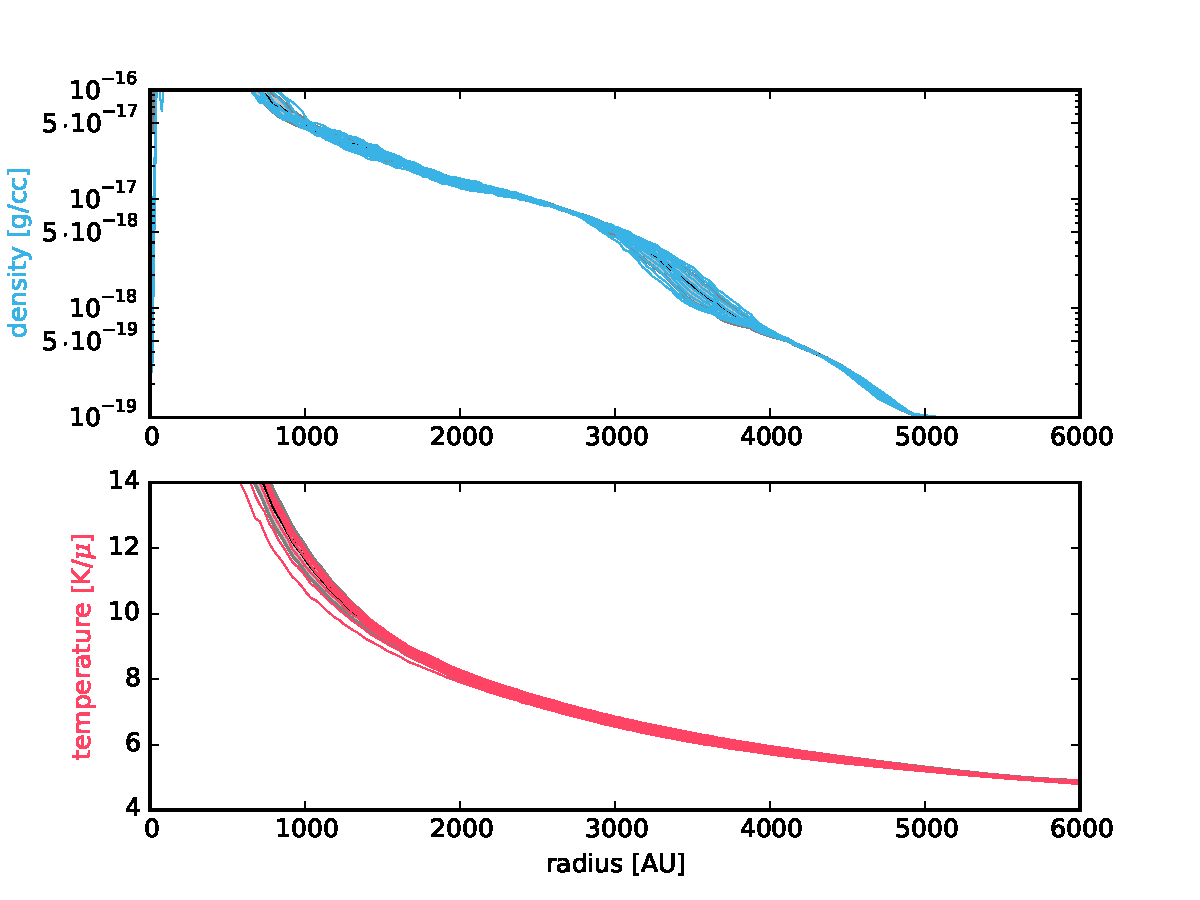
\includegraphics[width=0.99\textwidth]{Figures/var_rt_profiles/timeave_n100c01_6000AU}
 %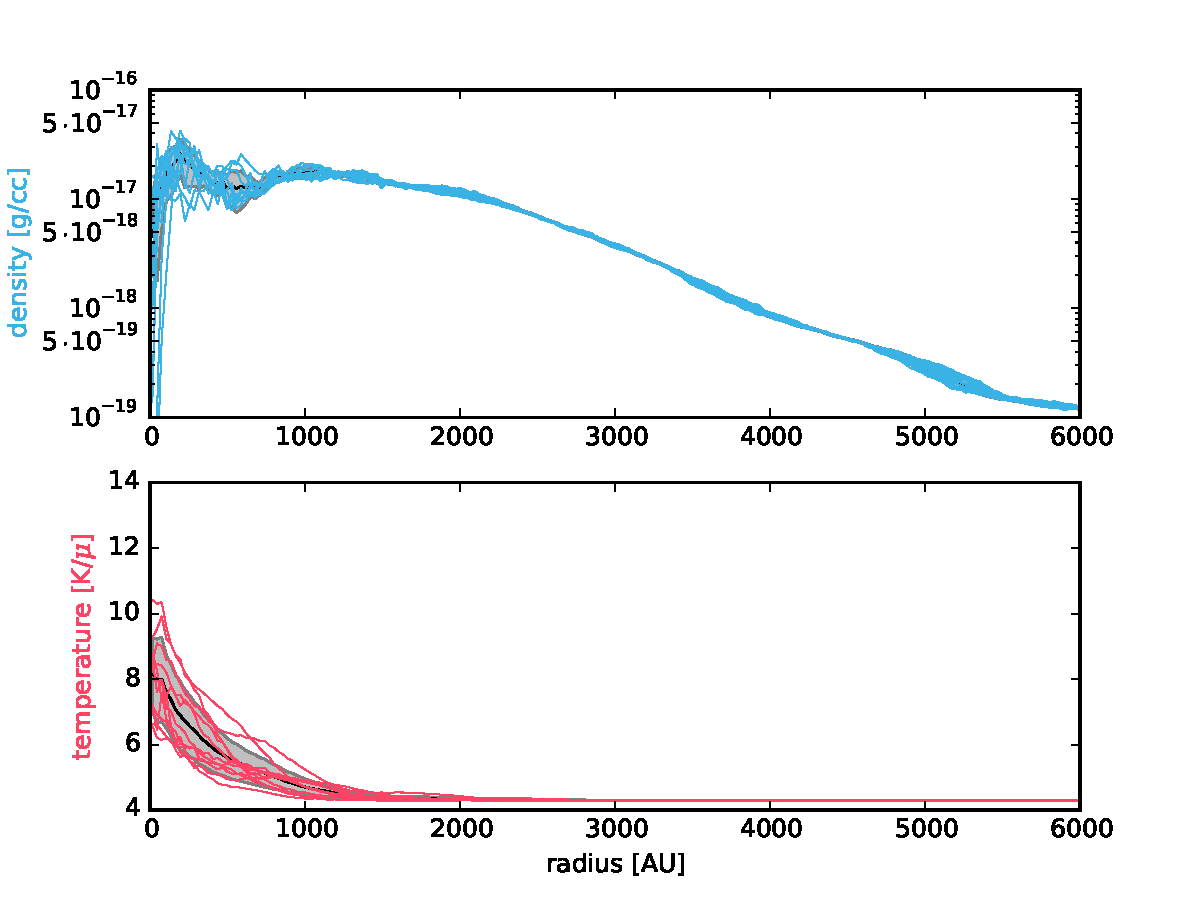
\includegraphics[width=0.99\textwidth]{Figures/var_rt_profiles/timeave_n100c1_6000AU}
 %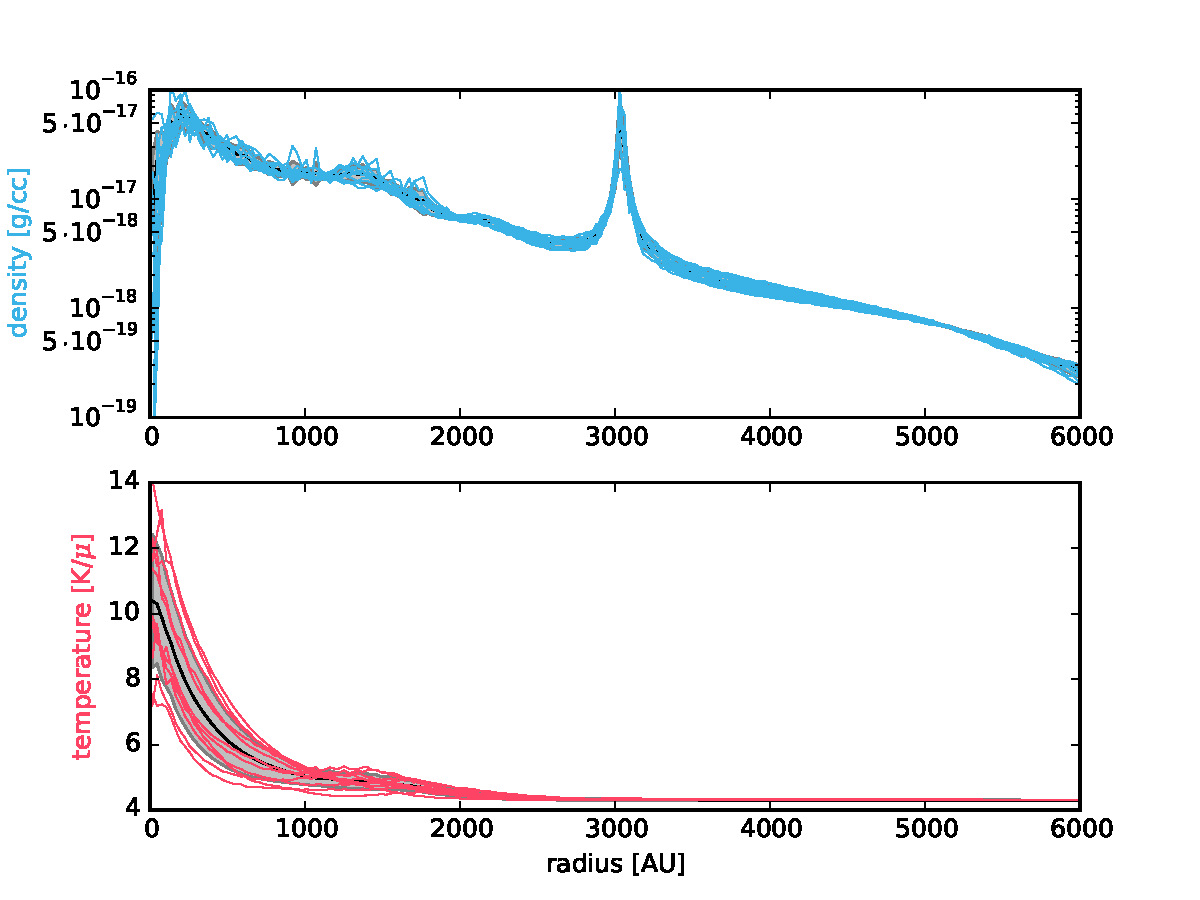
\includegraphics[width=0.99\textwidth]{Figures/var_rt_profiles/timeave_n100c10_6000AU}
 %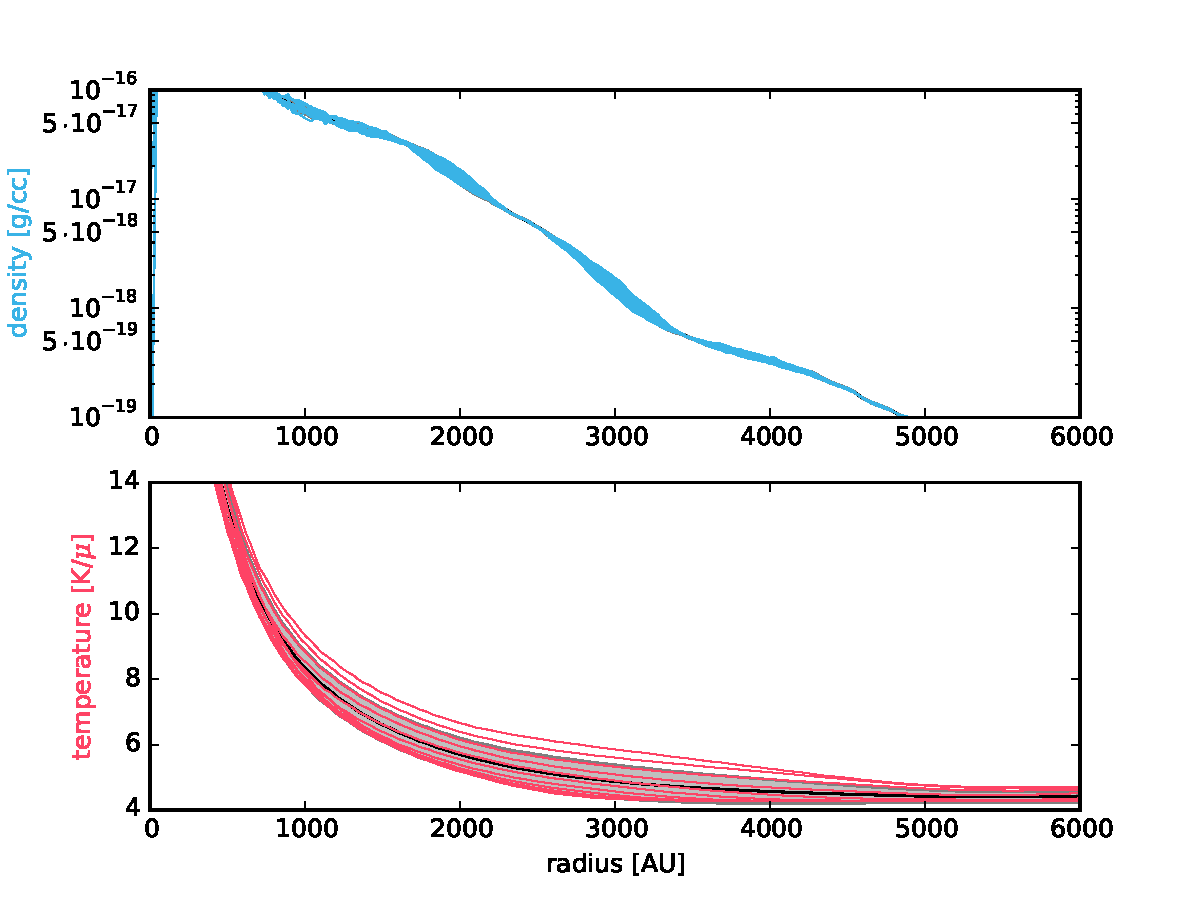
\includegraphics[width=0.99\textwidth]{Figures/var_rt_profiles/timeave_n10c01_6000AU}
 %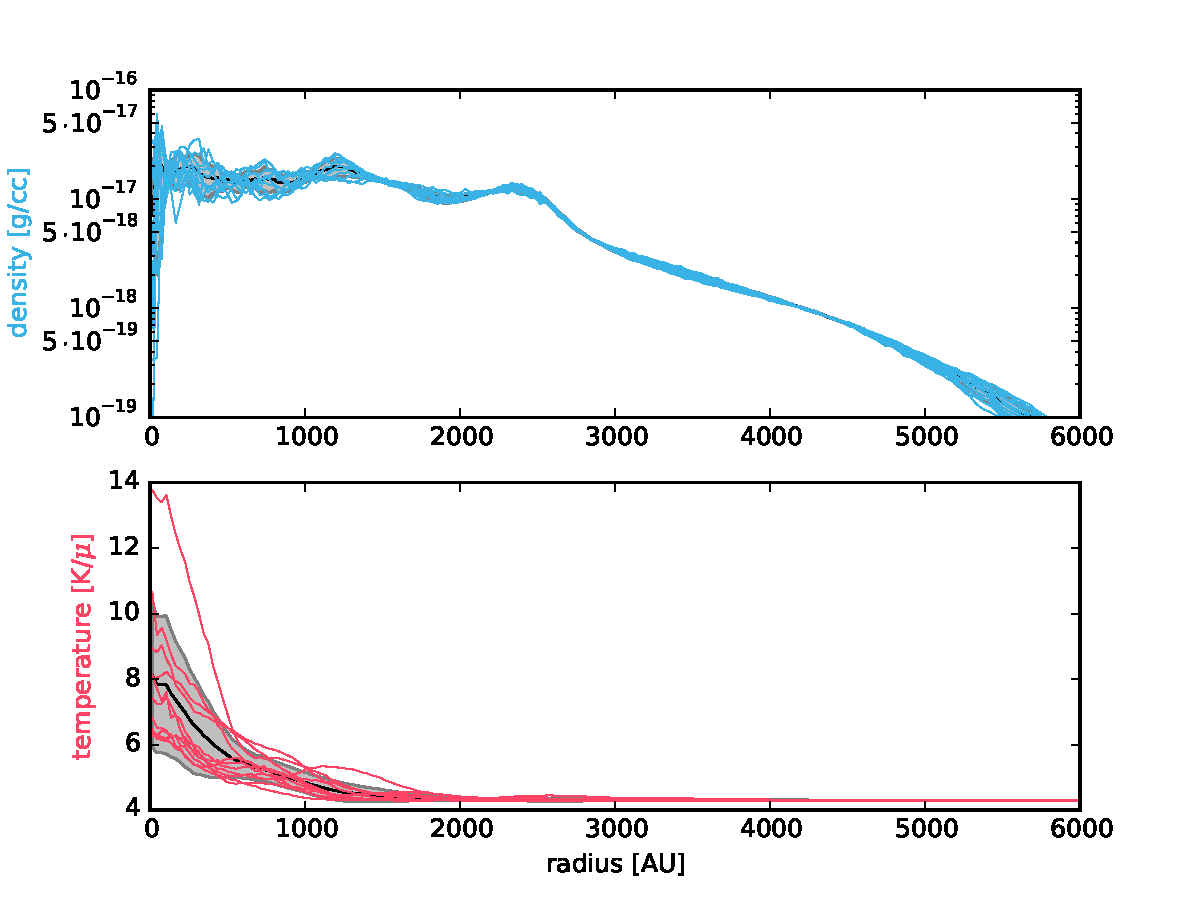
\includegraphics[width=0.99\textwidth]{Figures/var_rt_profiles/timeave_n10c1_6000AU}
 %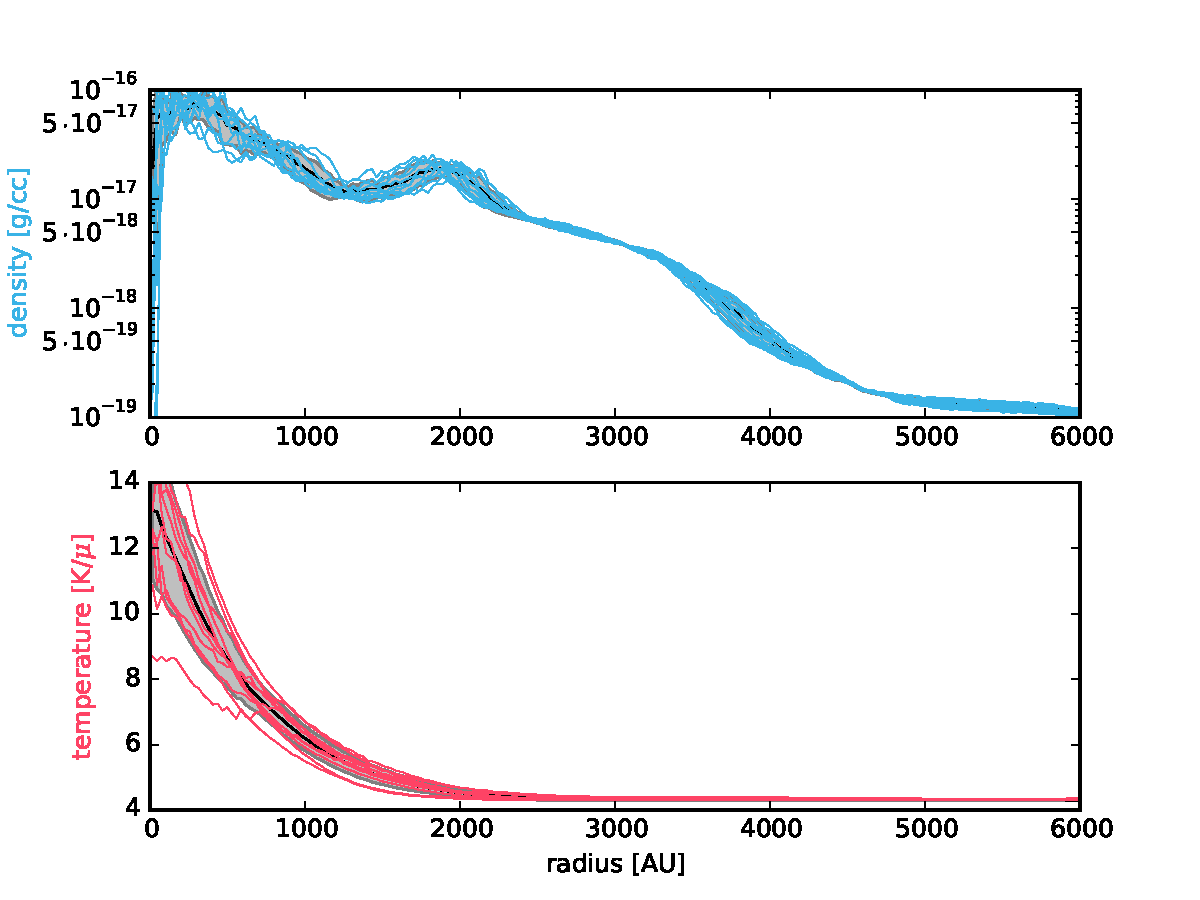
\includegraphics[width=0.99\textwidth]{Figures/var_rt_profiles/timeave_n10c10_6000AU}
 %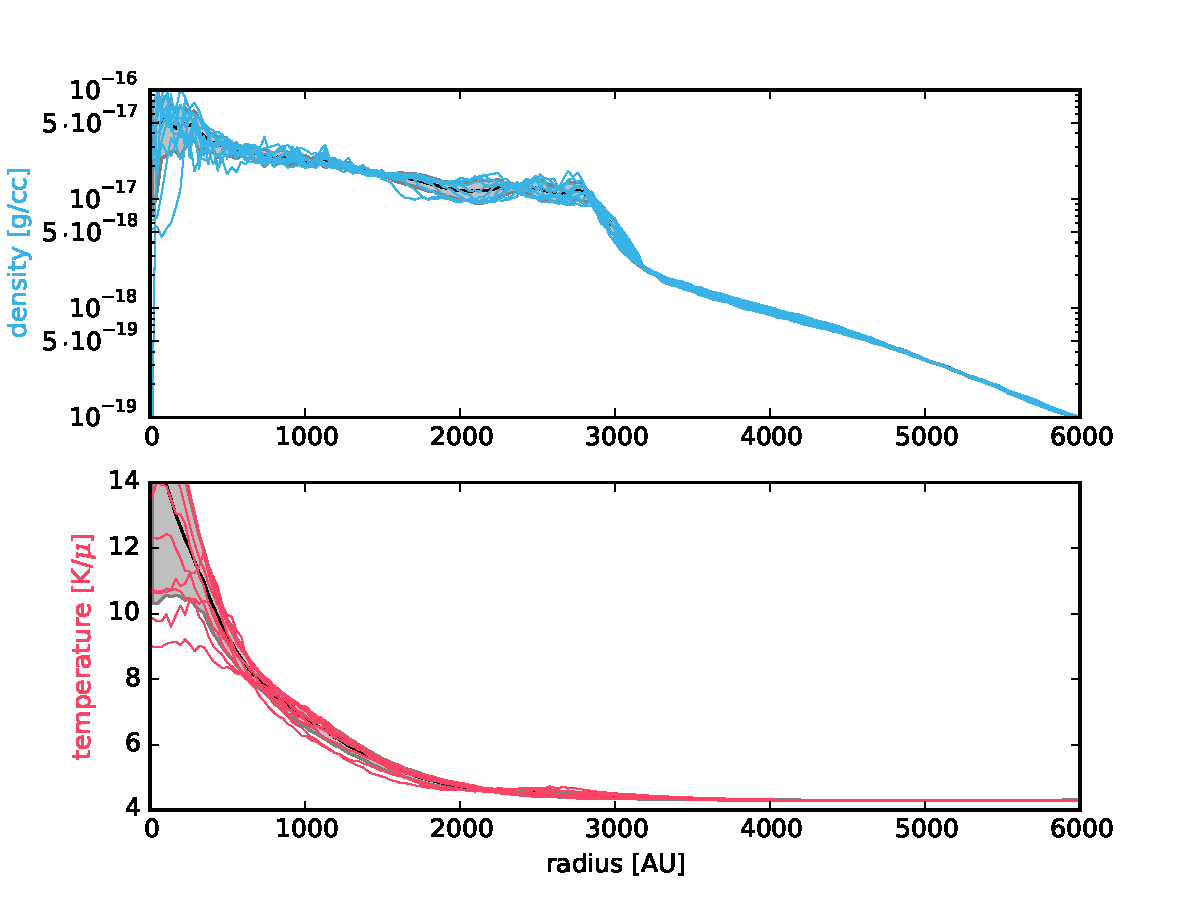
\includegraphics[width=0.99\textwidth]{Figures/var_rt_profiles/timeave_n1c01_6000AU}
 %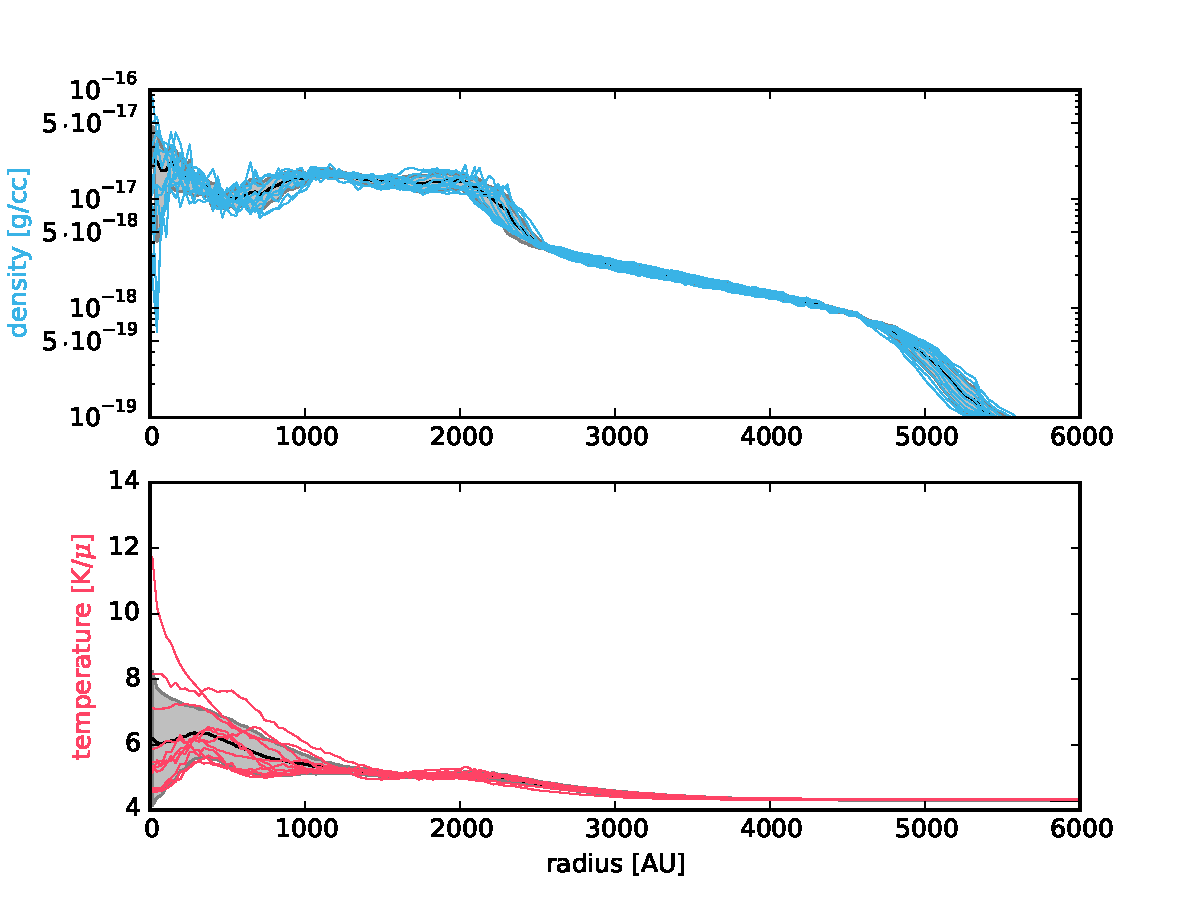
\includegraphics[width=0.99\textwidth]{Figures/var_rt_profiles/timeave_n1c1_6000AU}
 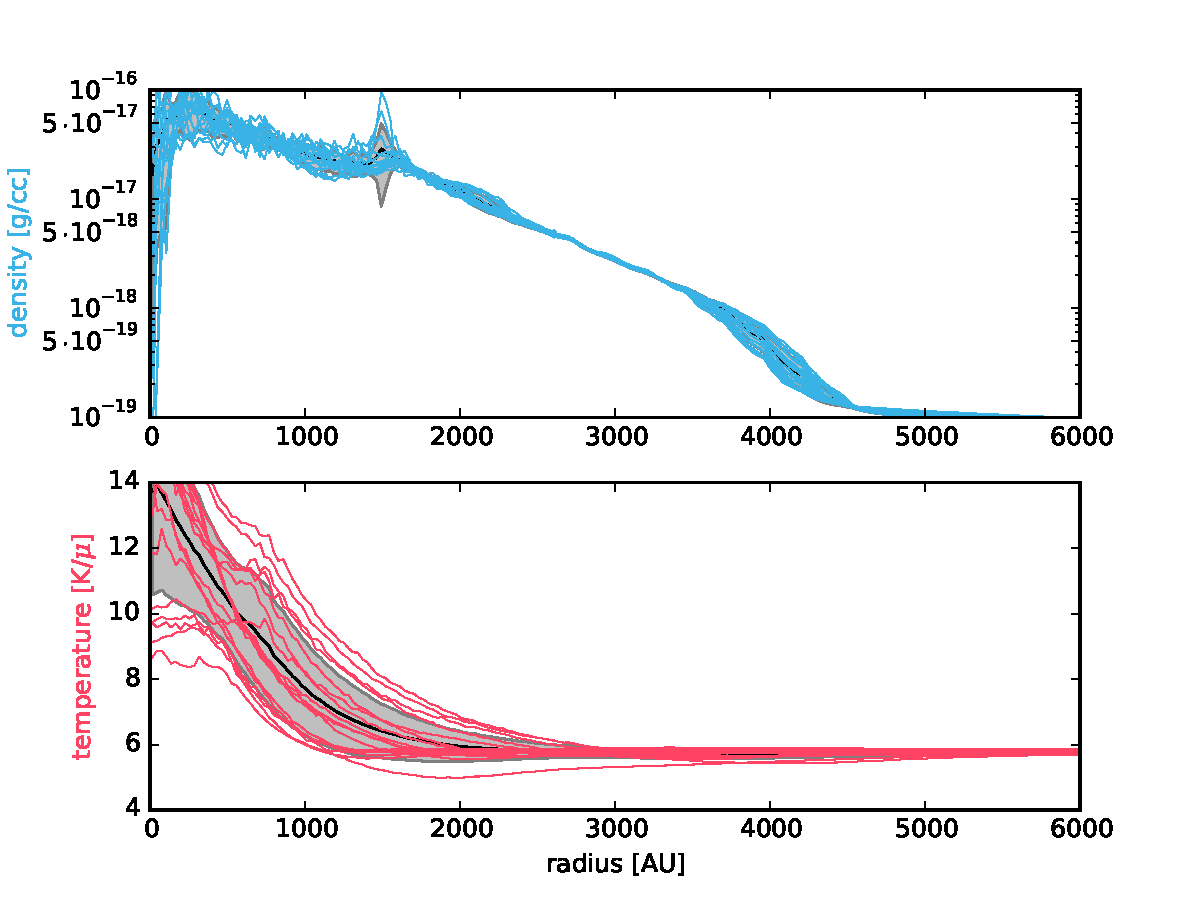
\includegraphics[width=1.0\textwidth]{Figures/var_rt_profiles/timeave_n1c10_6000AU_80_85kyrs}
 \captionsetup{justification=justified,singlelinecheck=false,width=\linewidth}
 \decoRule
 \caption[Density and temperature profiles]{Density and temperature profiles of \code{nsub1c10} run.
                                            The blue/red lines show the density/temperature profiles calculated at the last ten snapshots of the simulation at 80.49 to 85.50 kyrs.
                                            A grey--shaded area denotes the variance around the time--averaged value drawn as a black line.
                                            $\mu$ (with a value of around 2.3) denotes the molecular weight of the gas admixture of H, HII, H$_{2}$, and He.
                                            Centered around the most massive sink, a million points were randomly sampled within a radius of 6000 AU and a disk height of a few AU.
                                            These points were then histogrammed within concentrical shells.}
\label{fig:var_rt_profile}
\end{figure*}
\FloatBarrier

\begin{figure*}[!htb]
 \centering
 %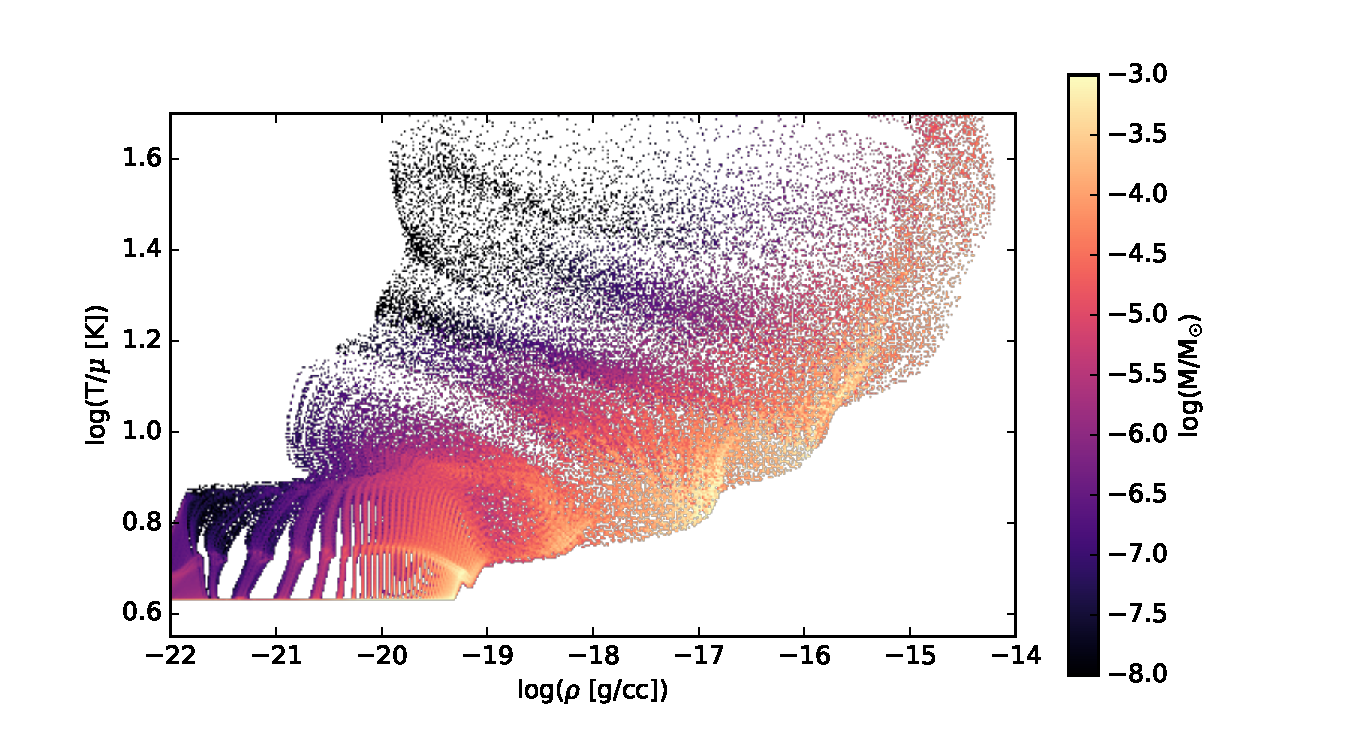
\includegraphics[width=0.99\textwidth]{Figures/var_rt_larson_plots/rho_temp_hist_n100c01}
 %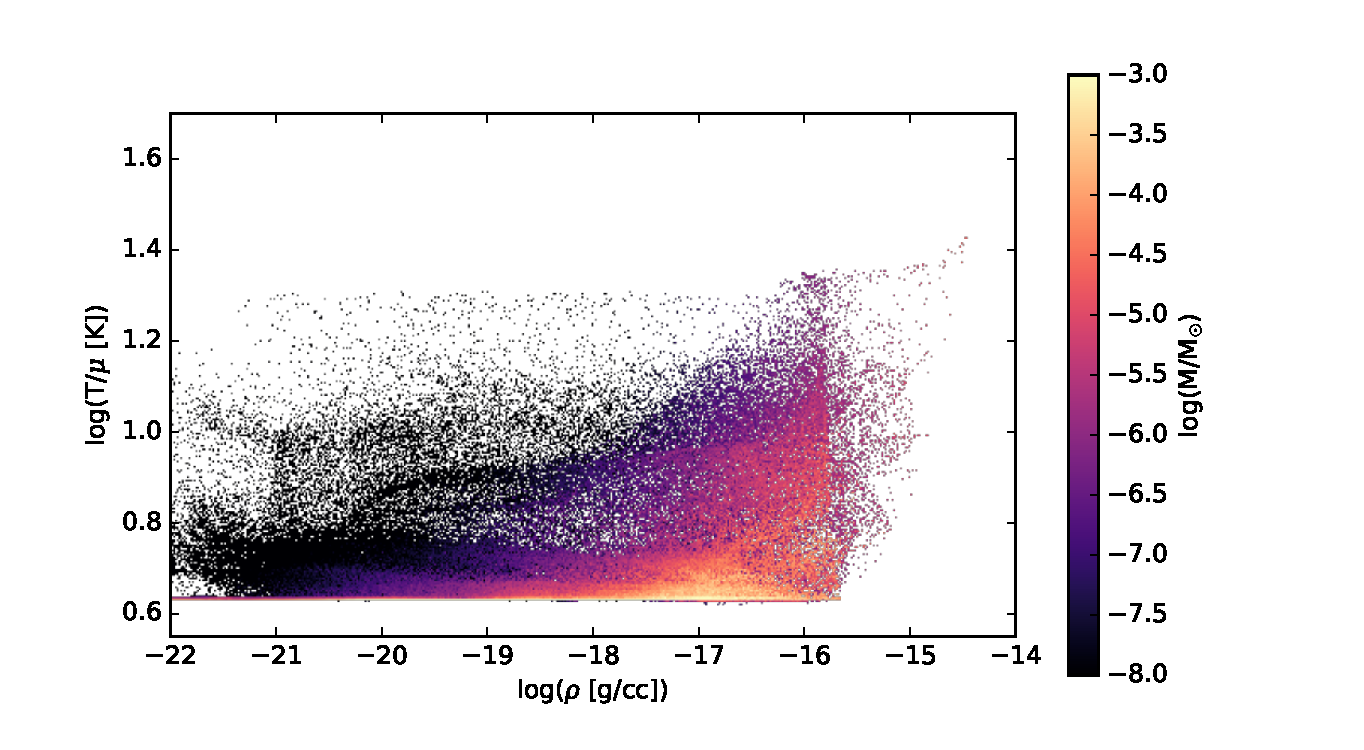
\includegraphics[width=0.99\textwidth]{Figures/var_rt_larson_plots/rho_temp_hist_n100c1}
 %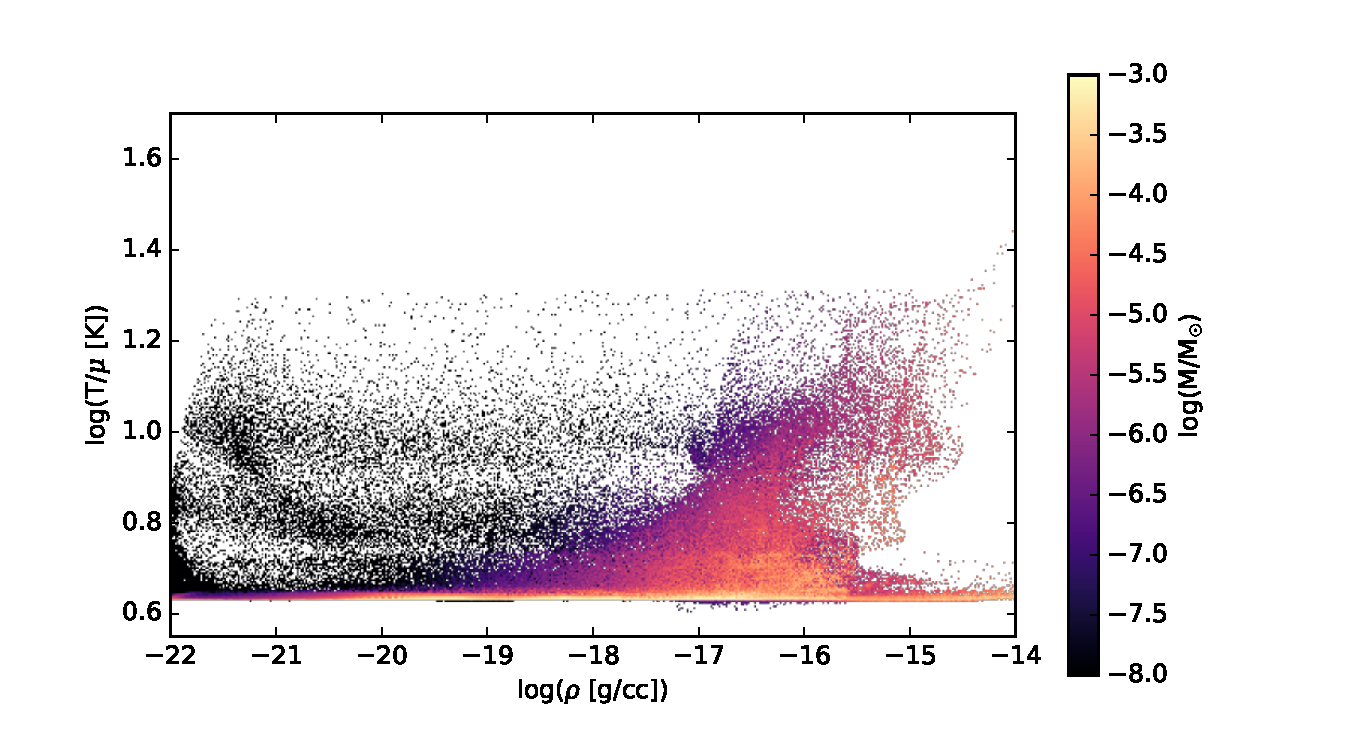
\includegraphics[width=0.99\textwidth]{Figures/var_rt_larson_plots/rho_temp_hist_n100c10}
 %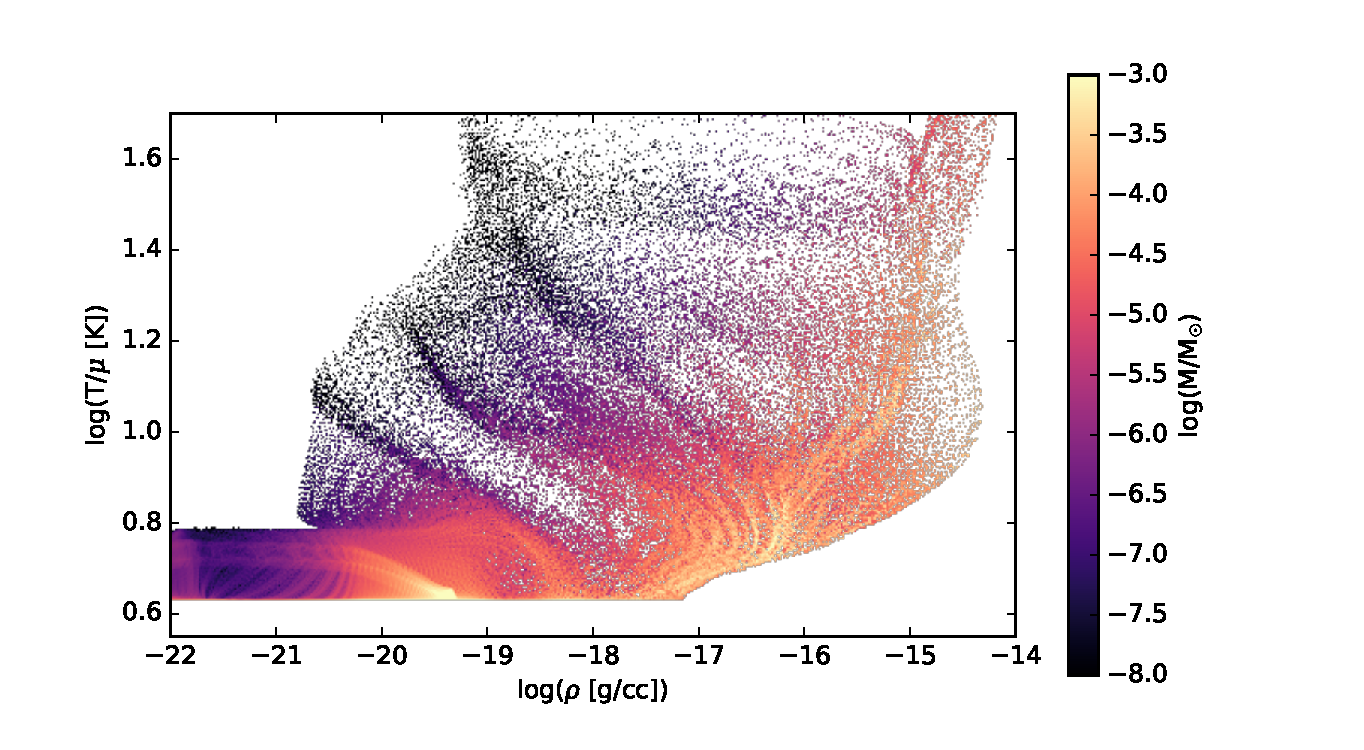
\includegraphics[width=0.99\textwidth]{Figures/var_rt_larson_plots/rho_temp_hist_n10c01}
 %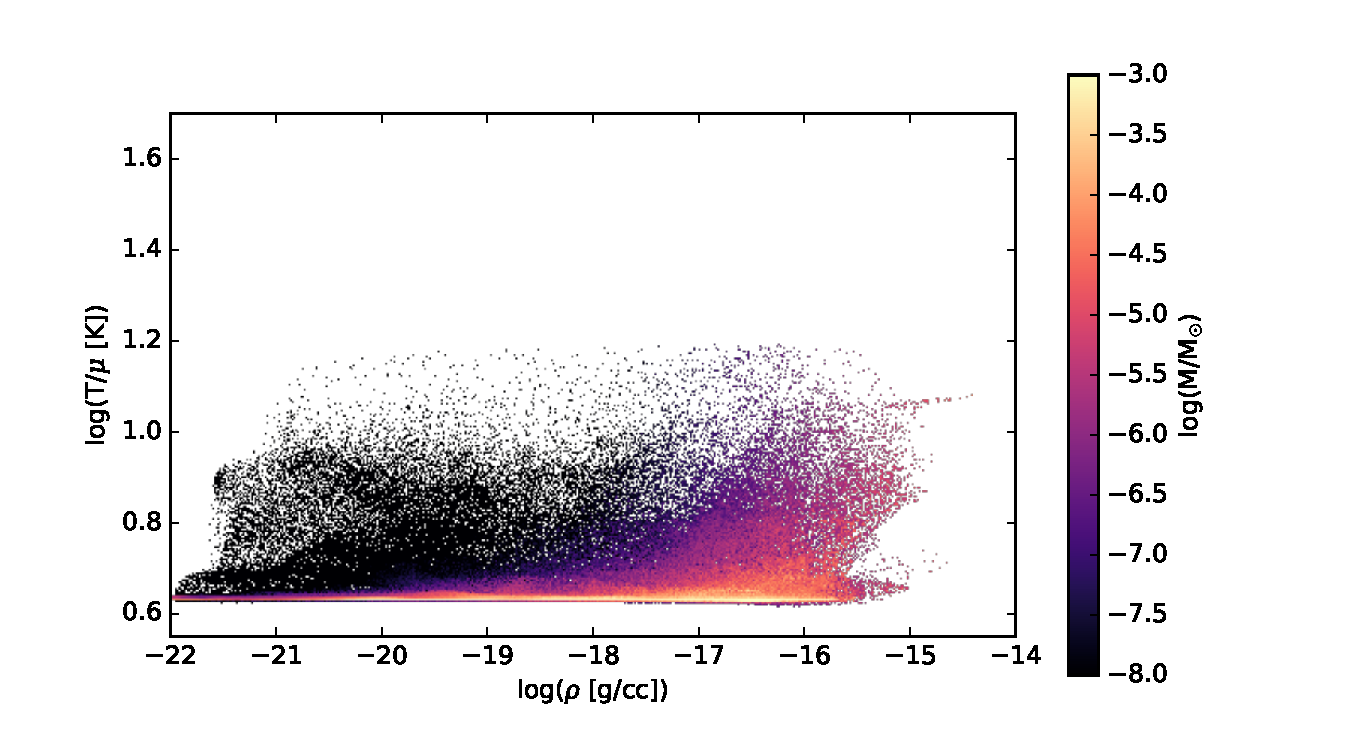
\includegraphics[width=0.99\textwidth]{Figures/var_rt_larson_plots/rho_temp_hist_n10c1}
 %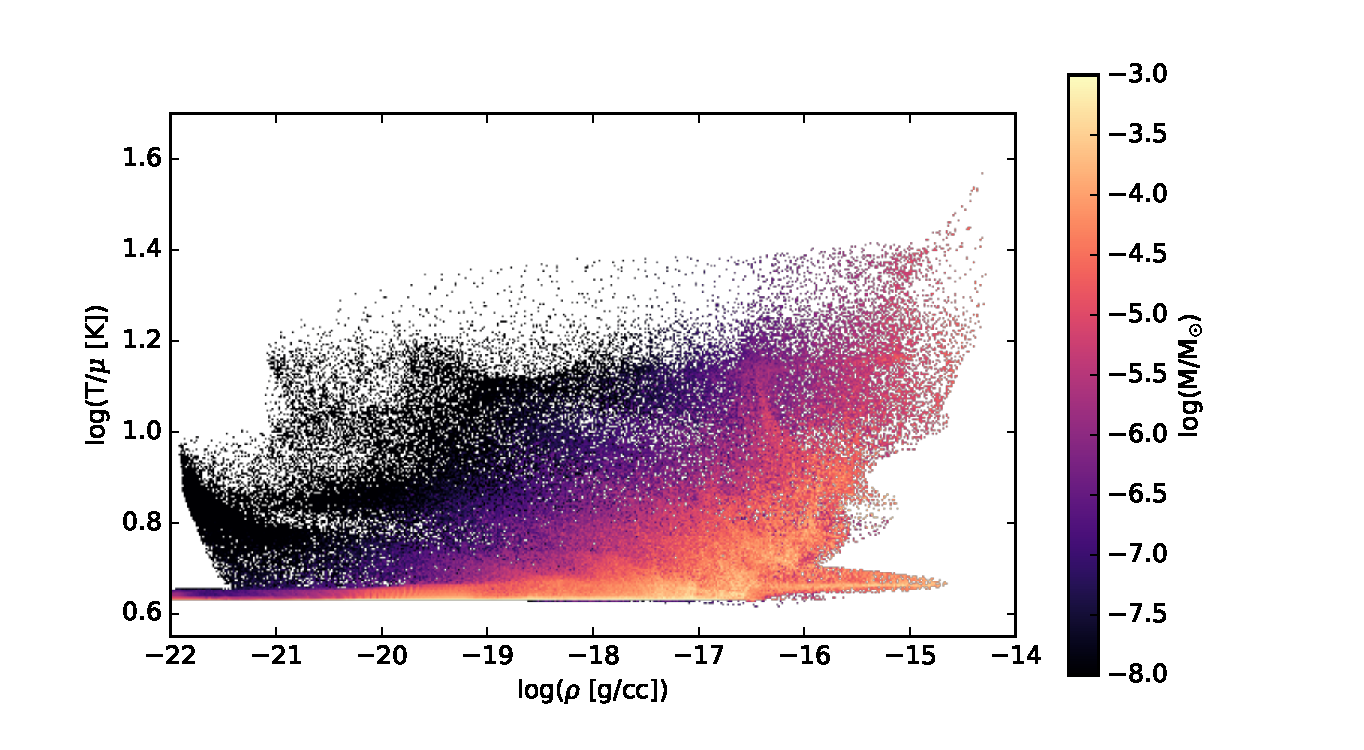
\includegraphics[width=0.99\textwidth]{Figures/var_rt_larson_plots/rho_temp_hist_n10c10}
 %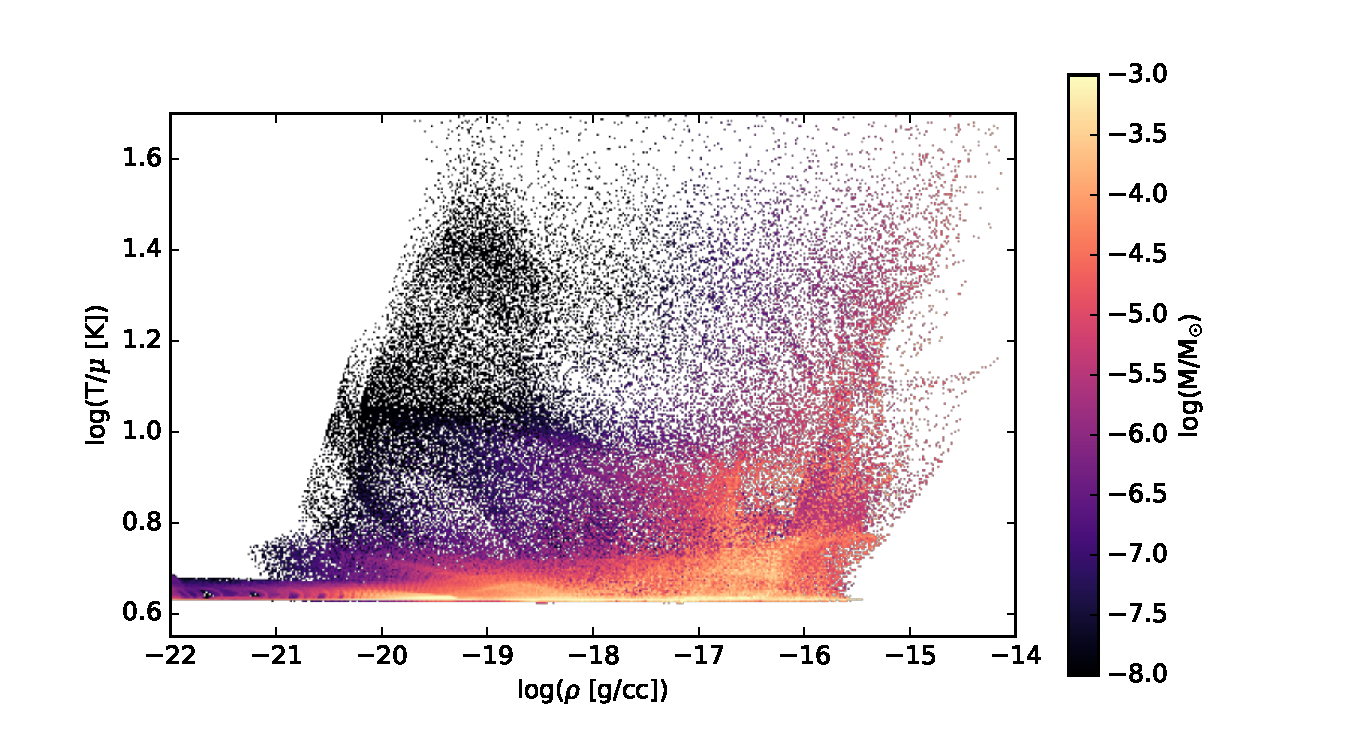
\includegraphics[width=0.99\textwidth]{Figures/var_rt_larson_plots/rho_temp_hist_n1c01}
 %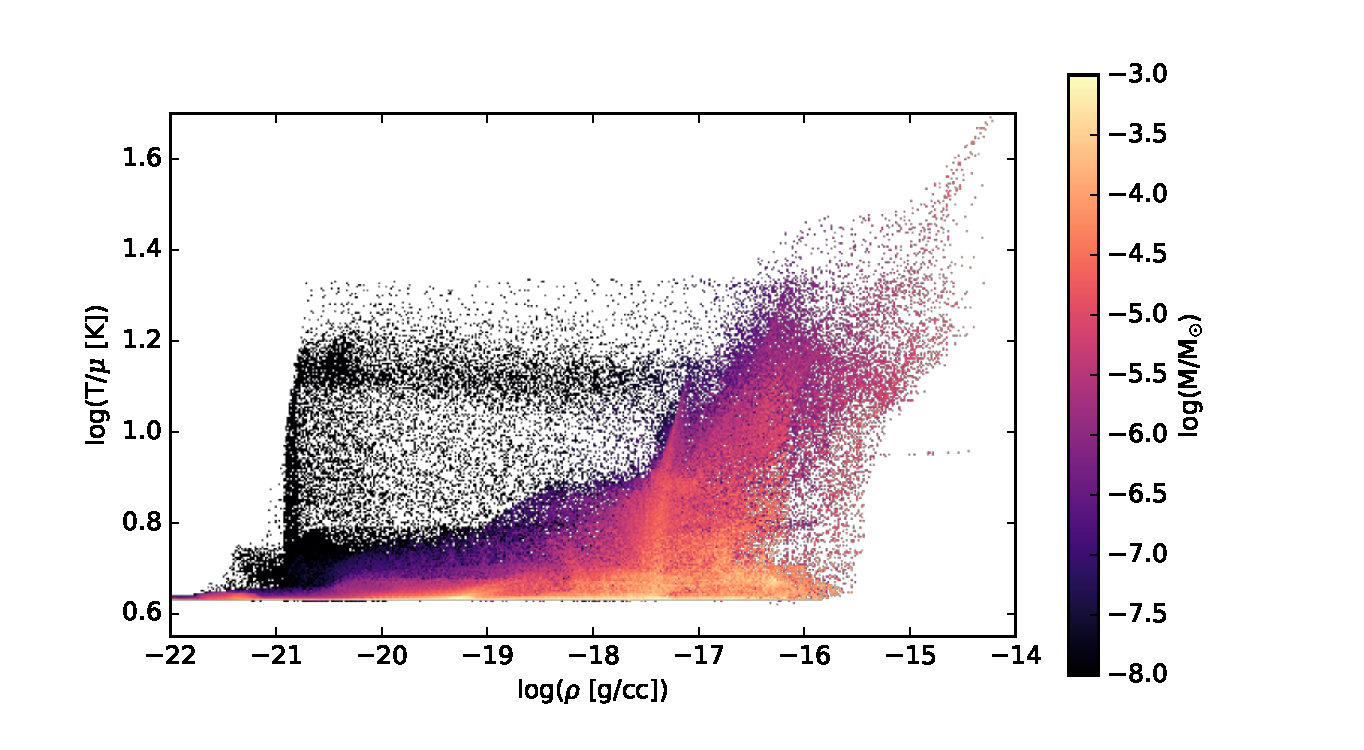
\includegraphics[width=0.99\textwidth]{Figures/var_rt_larson_plots/rho_temp_hist_n1c1}
 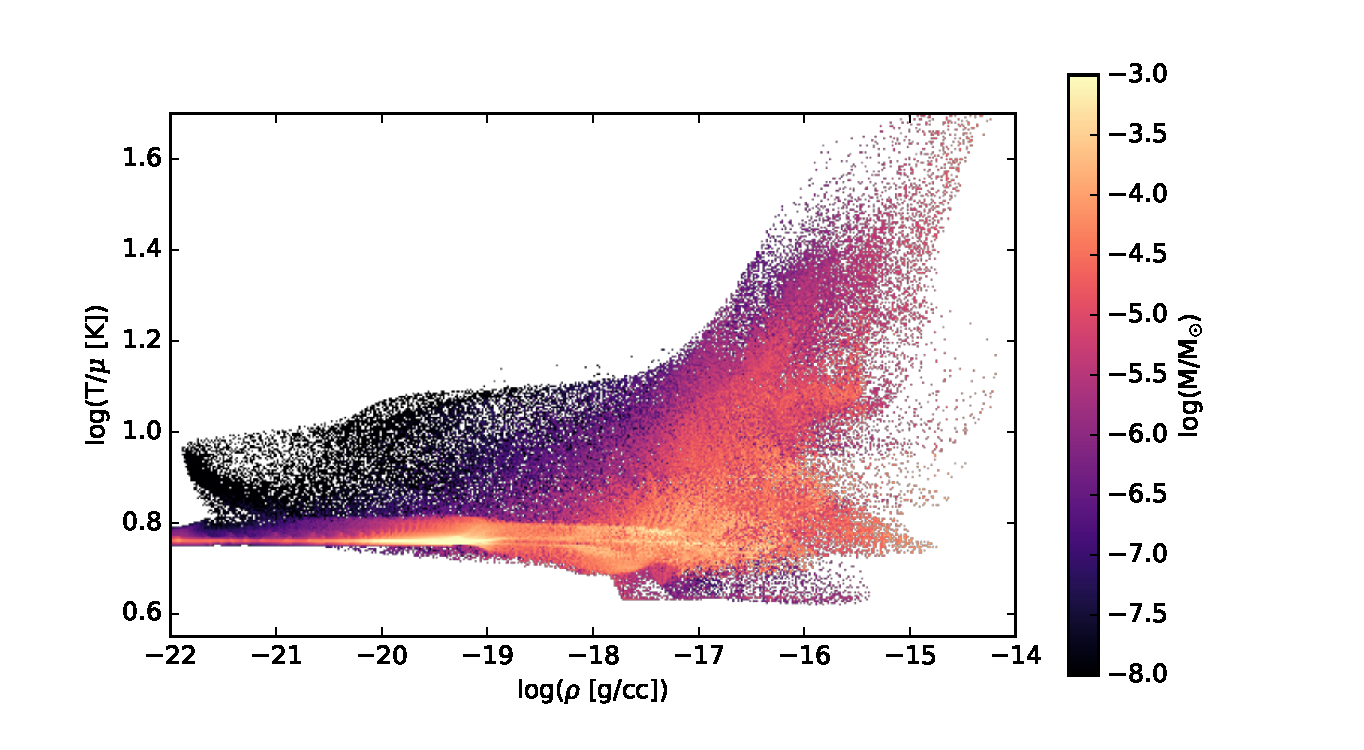
\includegraphics[width=1.0\textwidth]{Figures/var_rt_larson_plots/rho_temp_hist_n1c10}
 \captionsetup{justification=justified,singlelinecheck=false,width=\linewidth}
 \decoRule
 \caption[$\rho$--T phase diagram]{Density--temperature phase space diagram of \code{nsub1c10} run at 85.50 kyrs.
 %TODO
                                   Most of the mass follows on average the profile described by a polytropic EOS; see \secref{sec:Reference_runs}.
                                   At a knee density determined by the point where the optical depth crosses the opacity limit $\tau \simeq 1$, the radiation starts to become trapped and heats up the gas.
                                   At this point the first Larson core has formed; see \secref{subsec:Larson_cores}.}
\label{fig:var_rt_larson_rhoT}
\end{figure*}
\FloatBarrier


% other profiles ----------------------------------------------------------------------------------------
\subsubsection{Compilation of further profiles}
Here, all density and temperature profiles from the runs with variable reduced speed of light are shown.
The profiles are calculated within a disk radius of 6000 AU centered around the most massive sink in each simulation.
Within a relatively low disk height, a million sampling points are randomly selected and histogrammed in concentric shells.

This is done for the last ten snapshots of the simulation, which corresponds to a simulated time of 94.55 to 99.56 kyrs for all simulations, but one.
Run \code{nsub001c10} was unfortunately unable to reach the same time, since the time steps within the simulation became so small that the simulation virtually came to a halt.
Therefore the profiles for \code{nsub001c10} were calculated from a simulated time of 80.49 to 85.50 kyrs.

The blue curves show the density profiles for different snapshots, whereas the red curves show the temperature profiles for the same times.
The grey--shaded area shows the variance of the snapshots centered around the time average in black.

Another interesting analytical tool are phase space diagrams.
Phase space diagrams can show how thermodynamical properties of the simulation are related to each other.
Following the profiles, the mass--weighted phase space diagrams between density, temperature, and radius of the same runs are presented, again centered around the most massive sink.
They are calculated for every cell in a snapshot at a simulation time of 99.56 kyrs, except for the one of run \code{nsub001c10}, which was taken at 85.5 kyrs.
The radial phase space diagrams show peaks at certain radii representing sinks which accrete mass and heat up their surroundings.


% Profiles ----------------------------------------------------------------------------------------
% 0.1 c_frac_speed_factor

\begin{figure*}[!htb]
 \centering
 \includegraphics[width=0.95\textwidth]{Figures/var_rt_profiles/timeave_n100c01_6000AU}
 %\includegraphics[width=0.99\textwidth]{Figures/var_rt_profiles/timeave_n100c1_6000AU}
 %\includegraphics[width=0.99\textwidth]{Figures/var_rt_profiles/timeave_n100c10_6000AU}
 %\includegraphics[width=0.99\textwidth]{Figures/var_rt_profiles/timeave_n10c01_6000AU}
 %\includegraphics[width=0.99\textwidth]{Figures/var_rt_profiles/timeave_n10c1_6000AU}
 %\includegraphics[width=0.99\textwidth]{Figures/var_rt_profiles/timeave_n10c10_6000AU}
 %\includegraphics[width=0.99\textwidth]{Figures/var_rt_profiles/timeave_n1c01_6000AU}
 %\includegraphics[width=0.99\textwidth]{Figures/var_rt_profiles/timeave_n1c1_6000AU}
 %\includegraphics[width=0.99\textwidth]{Figures/var_rt_profiles/timeave_n1c10_6000AU_80_85kyrs}
 \captionsetup{justification=justified,singlelinecheck=false,width=\linewidth}
 \decoRule
 \caption[\code{nsub100c0.1} profiles]{Density and temperature profile of the \code{nsub100c0.1} run}
\label{fig:n100c0.1_profile}
\end{figure*}
\FloatBarrier

\begin{figure*}[!htb]
 \centering
 %\includegraphics[width=0.99\textwidth]{Figures/var_rt_profiles/timeave_n100c01_6000AU}
 %\includegraphics[width=0.99\textwidth]{Figures/var_rt_profiles/timeave_n100c1_6000AU}
 %\includegraphics[width=0.99\textwidth]{Figures/var_rt_profiles/timeave_n100c10_6000AU}
 \includegraphics[width=0.99\textwidth]{Figures/var_rt_profiles/timeave_n10c01_6000AU}
 %\includegraphics[width=0.99\textwidth]{Figures/var_rt_profiles/timeave_n10c1_6000AU}
 %\includegraphics[width=0.99\textwidth]{Figures/var_rt_profiles/timeave_n10c10_6000AU}
 %\includegraphics[width=0.99\textwidth]{Figures/var_rt_profiles/timeave_n1c01_6000AU}
 %\includegraphics[width=0.99\textwidth]{Figures/var_rt_profiles/timeave_n1c1_6000AU}
 %\includegraphics[width=0.99\textwidth]{Figures/var_rt_profiles/timeave_n1c10_6000AU_80_85kyrs}
 \captionsetup{justification=justified,singlelinecheck=false,width=\linewidth}
 \decoRule
 \caption[\code{nsub010c0.1} profiles]{Density and temperature profile of the \code{nsub010c0.1} run}
\label{fig:n10c0.1_profile}
\end{figure*}
\FloatBarrier

\begin{figure*}[!htb]
 \centering
 %\includegraphics[width=0.99\textwidth]{Figures/var_rt_profiles/timeave_n100c01_6000AU}
 %\includegraphics[width=0.99\textwidth]{Figures/var_rt_profiles/timeave_n100c1_6000AU}
 %\includegraphics[width=0.99\textwidth]{Figures/var_rt_profiles/timeave_n100c10_6000AU}
 %\includegraphics[width=0.99\textwidth]{Figures/var_rt_profiles/timeave_n10c01_6000AU}
 %\includegraphics[width=0.99\textwidth]{Figures/var_rt_profiles/timeave_n10c1_6000AU}
 %\includegraphics[width=0.99\textwidth]{Figures/var_rt_profiles/timeave_n10c10_6000AU}
 \includegraphics[width=0.99\textwidth]{Figures/var_rt_profiles/timeave_n1c01_6000AU}
 %\includegraphics[width=0.99\textwidth]{Figures/var_rt_profiles/timeave_n1c1_6000AU}
 %\includegraphics[width=0.99\textwidth]{Figures/var_rt_profiles/timeave_n1c10_6000AU_80_85kyrs}
 \captionsetup{justification=justified,singlelinecheck=false,width=\linewidth}
 \decoRule
 \caption[\code{nsub001c0.1} profiles]{Density and temperature profile of the \code{nsub001c0.1} run}
\label{fig:n1c0.1_profile}
\end{figure*}
\FloatBarrier

% 1.0 c_frac_speed_factor

\begin{figure*}[!htb]
 \centering
 %\includegraphics[width=0.99\textwidth]{Figures/var_rt_profiles/timeave_n100c01_6000AU}
 \includegraphics[width=0.99\textwidth]{Figures/var_rt_profiles/timeave_n100c1_6000AU}
 %\includegraphics[width=0.99\textwidth]{Figures/var_rt_profiles/timeave_n100c10_6000AU}
 %\includegraphics[width=0.99\textwidth]{Figures/var_rt_profiles/timeave_n10c01_6000AU}
 %\includegraphics[width=0.99\textwidth]{Figures/var_rt_profiles/timeave_n10c1_6000AU}
 %\includegraphics[width=0.99\textwidth]{Figures/var_rt_profiles/timeave_n10c10_6000AU}
 %\includegraphics[width=0.99\textwidth]{Figures/var_rt_profiles/timeave_n1c01_6000AU}
 %\includegraphics[width=0.99\textwidth]{Figures/var_rt_profiles/timeave_n1c1_6000AU}
 %\includegraphics[width=0.99\textwidth]{Figures/var_rt_profiles/timeave_n1c10_6000AU_80_85kyrs}
 \captionsetup{justification=justified,singlelinecheck=false,width=\linewidth}
 \decoRule
 \caption[\code{nsub100c1} profiles]{Density and temperature profile of the \code{nsub100c1} run}
\label{fig:n100c1.0_profile}
\end{figure*}
\FloatBarrier

\begin{figure*}[!htb]
 \centering
 %\includegraphics[width=0.99\textwidth]{Figures/var_rt_profiles/timeave_n100c01_6000AU}
 %\includegraphics[width=0.99\textwidth]{Figures/var_rt_profiles/timeave_n100c1_6000AU}
 %\includegraphics[width=0.99\textwidth]{Figures/var_rt_profiles/timeave_n100c10_6000AU}
 %\includegraphics[width=0.99\textwidth]{Figures/var_rt_profiles/timeave_n10c01_6000AU}
 \includegraphics[width=0.99\textwidth]{Figures/var_rt_profiles/timeave_n10c1_6000AU}
 %\includegraphics[width=0.99\textwidth]{Figures/var_rt_profiles/timeave_n10c10_6000AU}
 %\includegraphics[width=0.99\textwidth]{Figures/var_rt_profiles/timeave_n1c01_6000AU}
 %\includegraphics[width=0.99\textwidth]{Figures/var_rt_profiles/timeave_n1c1_6000AU}
 %\includegraphics[width=0.99\textwidth]{Figures/var_rt_profiles/timeave_n1c10_6000AU_80_85kyrs}
 \captionsetup{justification=justified,singlelinecheck=false,width=\linewidth}
 \decoRule
 \caption[\code{nsub010c1} profiles]{Density and temperature profile of the \code{nsub010c1} run}
\label{fig:n10c1.0_profile}
\end{figure*}
\FloatBarrier

\begin{figure*}[!htb]
 \centering
 %\includegraphics[width=0.99\textwidth]{Figures/var_rt_profiles/timeave_n100c01_6000AU}
 %\includegraphics[width=0.99\textwidth]{Figures/var_rt_profiles/timeave_n100c1_6000AU}
 %\includegraphics[width=0.99\textwidth]{Figures/var_rt_profiles/timeave_n100c10_6000AU}
 %\includegraphics[width=0.99\textwidth]{Figures/var_rt_profiles/timeave_n10c01_6000AU}
 %\includegraphics[width=0.99\textwidth]{Figures/var_rt_profiles/timeave_n10c1_6000AU}
 %\includegraphics[width=0.99\textwidth]{Figures/var_rt_profiles/timeave_n10c10_6000AU}
 %\includegraphics[width=0.99\textwidth]{Figures/var_rt_profiles/timeave_n1c01_6000AU}
 \includegraphics[width=0.99\textwidth]{Figures/var_rt_profiles/timeave_n1c1_6000AU}
 %\includegraphics[width=0.99\textwidth]{Figures/var_rt_profiles/timeave_n1c10_6000AU_80_85kyrs}
 \captionsetup{justification=justified,singlelinecheck=false,width=\linewidth}
 \decoRule
 \caption[\code{nsub001c1} profiles]{Density and temperature profile of the \code{nsub001c1} run}
\label{fig:n1c1.0_profile}
\end{figure*}
\FloatBarrier

% 10. c_frac_speed_factor

\begin{figure*}[!htb]
 \centering
 %\includegraphics[width=0.99\textwidth]{Figures/var_rt_profiles/timeave_n100c01_6000AU}
 %\includegraphics[width=0.99\textwidth]{Figures/var_rt_profiles/timeave_n100c1_6000AU}
 \includegraphics[width=0.99\textwidth]{Figures/var_rt_profiles/timeave_n100c10_6000AU}
 %\includegraphics[width=0.99\textwidth]{Figures/var_rt_profiles/timeave_n10c01_6000AU}
 %\includegraphics[width=0.99\textwidth]{Figures/var_rt_profiles/timeave_n10c1_6000AU}
 %\includegraphics[width=0.99\textwidth]{Figures/var_rt_profiles/timeave_n10c10_6000AU}
 %\includegraphics[width=0.99\textwidth]{Figures/var_rt_profiles/timeave_n1c01_6000AU}
 %\includegraphics[width=0.99\textwidth]{Figures/var_rt_profiles/timeave_n1c1_6000AU}
 %\includegraphics[width=0.99\textwidth]{Figures/var_rt_profiles/timeave_n1c10_6000AU_80_85kyrs}
 \captionsetup{justification=justified,singlelinecheck=false,width=\linewidth}
 \decoRule
 \caption[\code{nsub100c10} profiles]{Density and temperature profile of the \code{nsub100c10} run}
\label{fig:n100c10.0_profile}
\end{figure*}
\FloatBarrier


\begin{figure*}[!htb]
 \centering
 %\includegraphics[width=0.99\textwidth]{Figures/var_rt_profiles/timeave_n100c01_6000AU}
 %\includegraphics[width=0.99\textwidth]{Figures/var_rt_profiles/timeave_n100c1_6000AU}
 %\includegraphics[width=0.99\textwidth]{Figures/var_rt_profiles/timeave_n100c10_6000AU}
 %\includegraphics[width=0.99\textwidth]{Figures/var_rt_profiles/timeave_n10c01_6000AU}
 %\includegraphics[width=0.99\textwidth]{Figures/var_rt_profiles/timeave_n10c1_6000AU}
 \includegraphics[width=0.99\textwidth]{Figures/var_rt_profiles/timeave_n10c10_6000AU}
 %\includegraphics[width=0.99\textwidth]{Figures/var_rt_profiles/timeave_n1c01_6000AU}
 %\includegraphics[width=0.99\textwidth]{Figures/var_rt_profiles/timeave_n1c1_6000AU}
 %\includegraphics[width=0.99\textwidth]{Figures/var_rt_profiles/timeave_n1c10_6000AU_80_85kyrs}
 \captionsetup{justification=justified,singlelinecheck=false,width=\linewidth}
 \decoRule
 \caption[\code{nsub010c10} profiles]{Density and temperature profile of the \code{nsub010c10} run}
\label{fig:n10c10.0_profile}
\end{figure*}
\FloatBarrier

\begin{figure*}[!htb]
 \centering
 %\includegraphics[width=0.99\textwidth]{Figures/var_rt_profiles/timeave_n100c01_6000AU}
 %\includegraphics[width=0.99\textwidth]{Figures/var_rt_profiles/timeave_n100c1_6000AU}
 %\includegraphics[width=0.99\textwidth]{Figures/var_rt_profiles/timeave_n100c10_6000AU}
 %\includegraphics[width=0.99\textwidth]{Figures/var_rt_profiles/timeave_n10c01_6000AU}
 %\includegraphics[width=0.99\textwidth]{Figures/var_rt_profiles/timeave_n10c1_6000AU}
 %\includegraphics[width=0.99\textwidth]{Figures/var_rt_profiles/timeave_n10c10_6000AU}
 %\includegraphics[width=0.99\textwidth]{Figures/var_rt_profiles/timeave_n1c01_6000AU}
 %\includegraphics[width=0.99\textwidth]{Figures/var_rt_profiles/timeave_n1c1_6000AU}
 \includegraphics[width=0.99\textwidth]{Figures/var_rt_profiles/timeave_n1c10_6000AU_80_85kyrs}
 \captionsetup{justification=justified,singlelinecheck=false,width=\linewidth}
 \decoRule
 \caption[\code{nsub001c10} profiles]{Density and temperature profile of the \code{nsub001c10} run}
\label{fig:n1c10.0_profile}
\end{figure*}
\FloatBarrier


% Larson rho-T plots ----------------------------------------------------------------------------------------

\begin{figure*}[!htb]
 \centering
 \includegraphics[width=0.99\textwidth]{Figures/var_rt_larson_plots/rho_temp_hist_n100c01}
 %\includegraphics[width=0.99\textwidth]{Figures/var_rt_larson_plots/rho_temp_hist_n100c1}
 %\includegraphics[width=0.99\textwidth]{Figures/var_rt_larson_plots/rho_temp_hist_n100c10}
 \includegraphics[width=0.99\textwidth]{Figures/var_rt_larson_plots/rho_temp_hist_n10c01}
 %\includegraphics[width=0.99\textwidth]{Figures/var_rt_larson_plots/rho_temp_hist_n10c1}
 %\includegraphics[width=0.99\textwidth]{Figures/var_rt_larson_plots/rho_temp_hist_n10c10}
 \includegraphics[width=0.99\textwidth]{Figures/var_rt_larson_plots/rho_temp_hist_n1c01}
 %\includegraphics[width=0.99\textwidth]{Figures/var_rt_larson_plots/rho_temp_hist_n1c1}
 %\includegraphics[width=0.99\textwidth]{Figures/var_rt_larson_plots/rho_temp_hist_n1c10}
 \captionsetup{justification=justified,singlelinecheck=false,width=\linewidth}
 \decoRule
 \caption[\code{nsub*c0.1} $\rho$--T phase diagrams]{Density--temperature phase diagrams of runs \code{nsub100c0.1}, \code{nsub010c0.1} and \code{nsub001c0.1}}
\label{fig:c0.1_r_t_larson}
\end{figure*}
\FloatBarrier


\begin{figure*}[!htb]
 \centering
 %\includegraphics[width=0.99\textwidth]{Figures/var_rt_larson_plots/rho_temp_hist_n100c01}
 \includegraphics[width=0.99\textwidth]{Figures/var_rt_larson_plots/rho_temp_hist_n100c1}
 %\includegraphics[width=0.99\textwidth]{Figures/var_rt_larson_plots/rho_temp_hist_n100c10}
 %\includegraphics[width=0.99\textwidth]{Figures/var_rt_larson_plots/rho_temp_hist_n10c01}
 \includegraphics[width=0.99\textwidth]{Figures/var_rt_larson_plots/rho_temp_hist_n10c1}
 %\includegraphics[width=0.99\textwidth]{Figures/var_rt_larson_plots/rho_temp_hist_n10c10}
 %\includegraphics[width=0.99\textwidth]{Figures/var_rt_larson_plots/rho_temp_hist_n1c01}
 \includegraphics[width=0.99\textwidth]{Figures/var_rt_larson_plots/rho_temp_hist_n1c1}
 %\includegraphics[width=0.99\textwidth]{Figures/var_rt_larson_plots/rho_temp_hist_n1c10}
 \captionsetup{justification=justified,singlelinecheck=false,width=\linewidth}
 \decoRule
 \caption[\code{nsub*c1} $\rho$--T phase diagrams]{Density--temperature phase space diagrams of runs \code{nsub100c1}, \code{nsub010c1} and \code{nsub001c1}}
\label{fig:c1.0_r_t_larson}
\end{figure*}
\FloatBarrier


\begin{figure*}[!htb]
 \centering
 %\includegraphics[width=0.99\textwidth]{Figures/var_rt_larson_plots/rho_temp_hist_n100c01}
 %\includegraphics[width=0.99\textwidth]{Figures/var_rt_larson_plots/rho_temp_hist_n100c1}
 \includegraphics[width=0.99\textwidth]{Figures/var_rt_larson_plots/rho_temp_hist_n100c10}
 %\includegraphics[width=0.99\textwidth]{Figures/var_rt_larson_plots/rho_temp_hist_n10c01}
 %\includegraphics[width=0.99\textwidth]{Figures/var_rt_larson_plots/rho_temp_hist_n10c1}
 \includegraphics[width=0.99\textwidth]{Figures/var_rt_larson_plots/rho_temp_hist_n10c10}
 %\includegraphics[width=0.99\textwidth]{Figures/var_rt_larson_plots/rho_temp_hist_n1c01}
 %\includegraphics[width=0.99\textwidth]{Figures/var_rt_larson_plots/rho_temp_hist_n1c1}
 \includegraphics[width=0.99\textwidth]{Figures/var_rt_larson_plots/rho_temp_hist_n1c10}
 \captionsetup{justification=justified,singlelinecheck=false,width=\linewidth}
 \decoRule
 \caption[\code{nsub*c10} $\rho$--T phase diagrams]{Density--temperature phase space diagrams of runs \code{nsub100c10}, \code{nsub010c10} and \code{nsub001c10}}
\label{fig:c10.0_r_t_larson}
\end{figure*}
\FloatBarrier


% Larson rho-R plots ----------------------------------------------------------------------------------------

\begin{figure*}[!htb]
 \centering
 \includegraphics[width=0.99\textwidth]{Figures/var_rt_larson_plots/rho_R_hist_n100c01}
 %\includegraphics[width=0.99\textwidth]{Figures/var_rt_larson_plots/rho_R_hist_n100c1}
 %\includegraphics[width=0.99\textwidth]{Figures/var_rt_larson_plots/rho_R_hist_n100c10}
 \includegraphics[width=0.99\textwidth]{Figures/var_rt_larson_plots/rho_R_hist_n10c01}
 %\includegraphics[width=0.99\textwidth]{Figures/var_rt_larson_plots/rho_R_hist_n10c1}
 %\includegraphics[width=0.99\textwidth]{Figures/var_rt_larson_plots/rho_R_hist_n10c10}
 \includegraphics[width=0.99\textwidth]{Figures/var_rt_larson_plots/rho_R_hist_n1c01}
 %\includegraphics[width=0.99\textwidth]{Figures/var_rt_larson_plots/rho_R_hist_n1c1}
 %\includegraphics[width=0.99\textwidth]{Figures/var_rt_larson_plots/rho_R_hist_n1c10}
 \captionsetup{justification=justified,singlelinecheck=false,width=\linewidth}
 \decoRule
 \caption[\code{nsub*c0.1} $\rho$--R phase diagrams]{Density--radius phase space diagrams of runs \code{nsub100c0.1}, \code{nsub010c0.1} and \code{nsub001c0.1}}
\label{fig:c0.1_r_R_larson}
\end{figure*}
\FloatBarrier

\begin{figure*}[!htb]
 \centering
 %\includegraphics[width=0.99\textwidth]{Figures/var_rt_larson_plots/rho_R_hist_n100c01}
 \includegraphics[width=0.99\textwidth]{Figures/var_rt_larson_plots/rho_R_hist_n100c1}
 %\includegraphics[width=0.99\textwidth]{Figures/var_rt_larson_plots/rho_R_hist_n100c10}
 %\includegraphics[width=0.99\textwidth]{Figures/var_rt_larson_plots/rho_R_hist_n10c01}
 \includegraphics[width=0.99\textwidth]{Figures/var_rt_larson_plots/rho_R_hist_n10c1}
 %\includegraphics[width=0.99\textwidth]{Figures/var_rt_larson_plots/rho_R_hist_n10c10}
 %\includegraphics[width=0.99\textwidth]{Figures/var_rt_larson_plots/rho_R_hist_n1c01}
 \includegraphics[width=0.99\textwidth]{Figures/var_rt_larson_plots/rho_R_hist_n1c1}
 %\includegraphics[width=0.99\textwidth]{Figures/var_rt_larson_plots/rho_R_hist_n1c10}
 \captionsetup{justification=justified,singlelinecheck=false,width=\linewidth}
 \decoRule
 \caption[\code{nsub*c1} $\rho$--R phase diagrams]{Density--radius phase space diagrams of runs \code{nsub100c1}, \code{nsub010c1} and \code{nsub001c1}}
\label{fig:c1.0_r_R_larson}
\end{figure*}
\FloatBarrier

\begin{figure*}[!htb]
 \centering
 %\includegraphics[width=0.99\textwidth]{Figures/var_rt_larson_plots/rho_R_hist_n100c01}
 %\includegraphics[width=0.99\textwidth]{Figures/var_rt_larson_plots/rho_R_hist_n100c1}
 \includegraphics[width=0.99\textwidth]{Figures/var_rt_larson_plots/rho_R_hist_n100c10}
 %\includegraphics[width=0.99\textwidth]{Figures/var_rt_larson_plots/rho_R_hist_n10c01}
 %\includegraphics[width=0.99\textwidth]{Figures/var_rt_larson_plots/rho_R_hist_n10c1}
 \includegraphics[width=0.99\textwidth]{Figures/var_rt_larson_plots/rho_R_hist_n10c10}
 %\includegraphics[width=0.99\textwidth]{Figures/var_rt_larson_plots/rho_R_hist_n1c01}
 %\includegraphics[width=0.99\textwidth]{Figures/var_rt_larson_plots/rho_R_hist_n1c1}
 \includegraphics[width=0.99\textwidth]{Figures/var_rt_larson_plots/rho_R_hist_n1c10}
 \captionsetup{justification=justified,singlelinecheck=false,width=\linewidth}
 \decoRule
 \caption[\code{nsub*c10} $\rho$--R phase diagrams]{Density--radius phase space diagrams of runs \code{nsub100c10}, \code{nsub010c10} and \code{nsub001c10}}
\label{fig:c10.0_r_R_larson}
\end{figure*}
\FloatBarrier


% Larson T-R plots ----------------------------------------------------------------------------------------

\begin{figure*}[!htb]
 \centering
 \includegraphics[width=0.99\textwidth]{Figures/var_rt_larson_plots/temp_R_hist_n100c01}
 %\includegraphics[width=0.99\textwidth]{Figures/var_rt_larson_plots/temp_R_hist_n100c1}
 %\includegraphics[width=0.99\textwidth]{Figures/var_rt_larson_plots/temp_R_hist_n100c10}
 \includegraphics[width=0.99\textwidth]{Figures/var_rt_larson_plots/temp_R_hist_n10c01}
 %\includegraphics[width=0.99\textwidth]{Figures/var_rt_larson_plots/temp_R_hist_n10c1}
 %\includegraphics[width=0.99\textwidth]{Figures/var_rt_larson_plots/temp_R_hist_n10c10}
 \includegraphics[width=0.99\textwidth]{Figures/var_rt_larson_plots/temp_R_hist_n1c01}
 %\includegraphics[width=0.99\textwidth]{Figures/var_rt_larson_plots/temp_R_hist_n1c1}
 %\includegraphics[width=0.99\textwidth]{Figures/var_rt_larson_plots/temp_R_hist_n1c10}
 \captionsetup{justification=justified,singlelinecheck=false,width=\linewidth}
 \decoRule
 \caption[\code{nsub*c0.1} T--R phase diagrams]{Temperature--radius phase space diagrams of runs \code{nsub100c0.1}, \code{nsub010c0.1} and \code{nsub001c0.1}}
\label{fig:c0.1_T_R_larson}
\end{figure*}
\FloatBarrier

\begin{figure*}[!htb]
 \centering
 %\includegraphics[width=0.99\textwidth]{Figures/var_rt_larson_plots/temp_R_hist_n100c01}
 \includegraphics[width=0.99\textwidth]{Figures/var_rt_larson_plots/temp_R_hist_n100c1}
 %\includegraphics[width=0.99\textwidth]{Figures/var_rt_larson_plots/temp_R_hist_n100c10}
 %\includegraphics[width=0.99\textwidth]{Figures/var_rt_larson_plots/temp_R_hist_n10c01}
 \includegraphics[width=0.99\textwidth]{Figures/var_rt_larson_plots/temp_R_hist_n10c1}
 %\includegraphics[width=0.99\textwidth]{Figures/var_rt_larson_plots/temp_R_hist_n10c10}
 %\includegraphics[width=0.99\textwidth]{Figures/var_rt_larson_plots/temp_R_hist_n1c01}
 \includegraphics[width=0.99\textwidth]{Figures/var_rt_larson_plots/temp_R_hist_n1c1}
 %\includegraphics[width=0.99\textwidth]{Figures/var_rt_larson_plots/temp_R_hist_n1c10}
 \captionsetup{justification=justified,singlelinecheck=false,width=\linewidth}
 \decoRule
 \caption[\code{nsub*c1} T--R phase diagrams]{Temperature--radius phase space diagrams of runs \code{nsub100c1}, \code{nsub010c1} and \code{nsub001c1}}
\label{fig:c1.0_T_R_larson}
\end{figure*}
\FloatBarrier

\begin{figure*}[!htb]
 \centering
 %\includegraphics[width=0.99\textwidth]{Figures/var_rt_larson_plots/temp_R_hist_n100c01}
 %\includegraphics[width=0.99\textwidth]{Figures/var_rt_larson_plots/temp_R_hist_n100c1}
 \includegraphics[width=0.99\textwidth]{Figures/var_rt_larson_plots/temp_R_hist_n100c10}
 %\includegraphics[width=0.99\textwidth]{Figures/var_rt_larson_plots/temp_R_hist_n10c01}
 %\includegraphics[width=0.99\textwidth]{Figures/var_rt_larson_plots/temp_R_hist_n10c1}
 \includegraphics[width=0.99\textwidth]{Figures/var_rt_larson_plots/temp_R_hist_n10c10}
 %\includegraphics[width=0.99\textwidth]{Figures/var_rt_larson_plots/temp_R_hist_n1c01}
 %\includegraphics[width=0.99\textwidth]{Figures/var_rt_larson_plots/temp_R_hist_n1c1}
 \includegraphics[width=0.99\textwidth]{Figures/var_rt_larson_plots/temp_R_hist_n1c10}
 \captionsetup{justification=justified,singlelinecheck=false,width=\linewidth}
 \decoRule
 \caption[\code{nsub*c10} T--R phase diagrams]{Temperature--radius phase space diagrams of runs \code{nsub100c10}, \code{nsub010c10} and \code{nsub001c10}}
\label{fig:c10.0_T_R_larson}
\end{figure*}
\FloatBarrier

% !TEX root = ../main.tex
% Appendix E

\chapter{Overview} % Main appendix title

\label{sec:Overview}

On the next pages, Tables \ref{tab:hydro_pure}, \ref{tab:var_rt}, \ref{tab:const_rt}, \ref{tab:scaled}, and \ref{tab:selfsim} show an overview of all the relevant runs performed for the thesis, except the molecular cloud simulation.
The tables first lists some intrinsic properties of the simulation.
Next to them, the most important AMR parameters are listed.
Subsequently, some simulation results are displayed, such as the total number of sinks N$_{sinks}$, the total mass in sinks M$_{tot}$, or the most massive sink formed during the simulation M$_{sink}$.
rt\_c\_fraction and rt\_nsubcycle are also listed, since these are the parameters most thoroughly investigated.

\newpage
\thispagestyle{plain}
\begin{landscape}
 \begin{table}
\begin{adjustbox}{width=1.8\textheight}
\begin{tabular}{lcccccccccccccccc}
\toprule
Name ID & rt & pure\_hydro & isothermal & sink & merging [kyr] & L [AU] & levelmin & levelmax & ncpu & time [kyr] & duration [h] & N$_{sinks}$ & M$_{tot}$ [M$_{\odot}$] & M$_{sink}$ [M$_{\odot}$] & rt\_c\_fraction & rt\_nsubcycle \\
\midrule
hydro\_pure & .false. & .true. & .true. & .true. & 5 & 31999.92 & 7 & 12 & 32 & 3.03 & 7.89 & 39 & 0.38 & 0.27 & .false. & .false. \\
ref\_run & .false. & .true. & .true. & .true. & .false. & 31999.92 & 7 & 11 & 64 & 99.58 & 1.47 & 19 & 2.18 & 0.65 & .false. & .false. \\
ref\_l12 & .false. & .true. & .true. & .true. & .false. & 31999.92 & 7 & 12 & 32 & 116.47 & 4.30 & 24 & 2.49 & 0.51 & .false. & .false. \\
ref\_l13 & .false. & .true. & .true. & .true. & .false. & 31999.92 & 7 & 13 & 32 & 116.56 & 11.53 & 23 & 2.27 & 0.47 & .false. & .false. \\
ref\_l14 & .false. & .true. & .true. & .true. & 5 & 31999.92 & 7 & 14 & 64 & 112.55 & 35.20 & 25 & 2.11 & 0.83 & .false. & .false. \\
merge\_on & .false. & .true. & .true. & .true. & 5 & 31999.92 & 7 & 12 & 64 & 6.13 & 22.34 & 12 & 0.73 & 0.53 & .false. & .false. \\
no\_merge & .false. & .true. & .true. & .true. & .false. & 31999.92 & 7 & 12 & 64 & 4.59 & 3.47 & 8 & 0.55 & 0.37 & .false. & .false. \\
\bottomrule
\end{tabular}
\end{adjustbox}
\caption[Large--sphere runs]{Summary of all pure--hydrodynamics runs with a 4\,M$_{\odot}$ non--singular isothermal sphere profile. \\
														 These runs can be used as reference for radiation hydrodynamics simulations.}
\label{tab:hydro_pure}
\end{table}

 \begin{table}
\begin{adjustbox}{width=1.8\textheight}
\begin{tabular}{lccccccccccccccccc}
\toprule
Name ID & rt & pure\_hydro & isothermal & sink & merging [kyr] & L [AU] & levelmin & levelmax & ncpu & time [kyr] & duration [h] & N$_{sinks}$ & M$_{tot}$ [M$_{\odot}$] & M$_{sink}$ [M$_{\odot}$] & rt\_c\_fraction & rt\_nsubcycle & c\_frac\_speed\_factor \\
\midrule
nsub001c0.1 & .true. & .false. & .false. & .true. & .false. & 31999.92 & 7 & 11 & 16 & 99.62 & 3.33 & 6 & 1.70 & 1.05 & 1.0000e-05 & 1 & 0.1 \\
nsub001c1 & .true. & .false. & .false. & .true. & .false. & 31999.92 & 7 & 11 & 16 & 99.57 & 39.76 & 10 & 1.97 & 0.99 & 1.0000e-05 & 1 & 1.0 \\
nsub001c10 & .true. & .false. & .false. & .true. & .false. & 31999.92 & 7 & 11 & 128 & 85.56 & 245.81 & 3 & 0.89 & 0.97 & 1.0000e-05 & 1 & 10.0 \\
nsub010c0.1 & .true. & .false. & .false. & .true. & .false. & 31999.92 & 7 & 11 & 16 & 99.60 & 1.13 & 1 & 1.04 & 1.04 & 1.0000e-05 & 10 & 0.1 \\
nsub010c1 & .true. & .false. & .false. & .true. & .false. & 31999.92 & 7 & 11 & 16 & 99.64 & 7.82 & 17 & 1.90 & 1.01 & 1.0000e-05 & 10 & 1.0 \\
nsub010c10 & .true. & .false. & .false. & .true. & .false. & 31999.92 & 7 & 11 & 16 & 99.58 & 106.91 & 11 & 1.62 & 1.01 & 1.0000e-05 & 10 & 10.0 \\
nsub100c0.1 & .true. & .false. & .false. & .true. & .false. & 31999.92 & 7 & 11 & 16 & 99.63 & 1.02 & 1 & 1.01 & 1.00 & 1.0000e-05 & 100 & 0.1 \\
nsub100c1 & .true. & .false. & .false. & .true. & .false. & 31999.92 & 7 & 11 & 16 & 99.59 & 7.97 & 11 & 1.94 & 1.05 & 1.0000e-05 & 100 & 1.0 \\
nsub100c10 & .true. & .false. & .false. & .true. & .false. & 31999.92 & 7 & 11 & 16 & 99.62 & 89.01 & 10 & 1.77 & 1.04 & 1.0000e-05 & 100 & 10.0 \\
\bottomrule
\end{tabular}
\end{adjustbox}
\caption[Variable speed of light runs]{Summary of all runs with variable reduced speed of light and a 4\,M$_{\odot}$ non--singular isothermal sphere profile.}
\label{tab:var_rt}
\end{table}

 \begin{table}
\begin{adjustbox}{width=1.8\textheight}
\begin{tabular}{lcccccccccccccccc}
\toprule
Name ID & rt & pure\_hydro & isothermal & sink & merging [kyr] & L [AU] & levelmin & levelmax & ncpu & time [kyr] & duration [h] & N$_{sinks}$ & M$_{tot}$ [M$_{\odot}$] & M$_{sink}$ [M$_{\odot}$] & rt\_c\_fraction & rt\_nsubcycle \\
\midrule
const\_rtc & .true. & .false. & .false. & .true. & .false. & 31999.92 & 7 & 11 & 64 & 99.58 & 52.11 & 9 & 1.87 & 1.06 & 1.4779e-04 & 1 \\
nsub\_const\_rtc & .true. & .false. & .false. & .true. & .false. & 31999.92 & 7 & 11 & 64 & 99.61 & 11.38 & 9 & 1.65 & 1.01 & 1.4779e-04 & 100 \\
nsub\_fast & .true. & .false. & .false. & .true. & .false. & 31999.92 & 7 & 11 & 64 & 99.61 & 72.30 & 5 & 1.29 & 1.06 & 1.4779e-03 & 100 \\
\bottomrule
\end{tabular}
\end{adjustbox}
\caption[Constant reduced speed of light runs]{Summary of all runs with a constant reduced speed of light and a 4\,M$_{\odot}$ non--singular isothermal sphere profile.}
\label{tab:const_rt}
\end{table}

\end{landscape}

\newpage
\thispagestyle{plain}
\begin{landscape}
 \begin{table}
\begin{adjustbox}{width=1.8\textheight}
\begin{tabular}{lcccccccccccccccc}
\toprule
Name ID & rt & pure\_hydro & isothermal & sink & merging [kyr] & L [AU] & levelmin & levelmax & ncpu & time [kyr] & duration [h] & N$_{sinks}$ & M$_{tot}$ [M$_{\odot}$] & M$_{sink}$ [M$_{\odot}$] & rt\_c\_fraction & rt\_nsubcycle \\
\midrule
scaled\_up\_iso & .false. & .true. & .true. & .true. & .false. & 799998.02 & 7 & 16 & 64 & 194.35 & 17.79 & 24 & 4.80 & 3.09 & .false. & .false. \\
scaled\_up\_iso2 & .false. & .true. & .true. & .true. & .false. & 799998.02 & 7 & 16 & 64 & 214.96 & 23.98 & 60 & 32.20 & 6.83 & .false. & .false. \\
scaled\_up\_iso\_merge & .false. & .true. & .true. & .true. & 5 & 799998.02 & 7 & 16 & 64 & 241.22 & 24.00 & 123 & 36.46 & 4.94 & .false. & .false. \\
scaled\_up\_iso\_merge2 & .false. & .true. & .true. & .true. & 5 & 799998.02 & 7 & 16 & 64 & 228.59 & 23.95 & 83 & 26.38 & 3.79 & .false. & .false. \\
scaled\_up\_plain & .false. & .true. & .true. & .false. & .false. & 799998.02 & 7 & 16 & 64 & 235.45 & 16.46 & 64 & 32.53 & 5.65 & .false. & .false. \\
scaled\_up\_plain\_nosinks & .false. & .true. & .true. & .false. & .false. & 799998.02 & 7 & 16 & 64 & 91.92 & 3.41 & 0 & 0 & 0 & .false. & .false. \\
scaled\_up\_nolacc & .false. & .true. & .true. & .false. & .false. & 799998.02 & 7 & 16 & 64 & 147.72 & 9.99 & 0 & 0 & 0 & .false. & .false. \\
scaled\_up\_test & .false. & .true. & .true. & .true. & 5 & 799998.02 & 7 & 16 & 64 & 267.43 & 23.97 & 55 & 32.81 & 5.29 & .false. & .false. \\
scaled\_up\_isoknee & .false. & .true. & .true.$^{\ast}$ & .false. & .false. & 799998.02 & 7 & 16 & 64 & 328.20 & 21.04 & 0 & 0 & 0 & .false. & .false. \\
scaled\_up\_isoknee\_sink & .false. & .true. & .true.$^{\ast}$ & .true. & 5 & 799998.02 & 7 & 16 & 64 & 328.07 & 20.39 & 17 & 51.45 & 19.39 & .false. & .false. \\
scaled\_up\_periodic & .false. & .true. & .true. & .true. & 5 & 799998.02 & 7 & 16 & 64 & 47.06 & 1.09 & 2 & 2.59 & 1.66 & .false. & .false. \\
scaled\_up\_lmin8 & .false. & .true. & .true.$^{\ast}$ & .false. & .false. & 799998.02 & 8 & 16 & 64 & 279.69 & 27.19 & 0 & 0 & 0 & .false. & .false. \\
scaled\_up\_msph & .false. & .true. & .true.$^{\ast}$ & .false. & .false. & 799998.02 & 7 & 16 & 64 & 296.34 & 23.94 & 0 & 0 & 0 & .false. & .false. \\
scaled\_up\_msphws & .false. & .true. & .true.$^{\ast}$ & .true. & 5 & 799998.02 & 7 & 16 & 64 & 293.94 & 23.98 & 14 & 45.34 & 14.79 & .false. & .false. \\
scaled\_up & .true. & .false. & .false. & .true. & 5 & 799998.02 & 7 & 16 & 256 & 278.84 & 24.00 & 2 & 41.82 & 28.74 & 1.4779e-03 & 100 \\
\bottomrule
\end{tabular}
\end{adjustbox}
\caption[High--resolution runs]{Summary of all runs with a physical resolution of 12.21\,AU and a 100\,M$_{\odot}$ non--singular isothermal sphere profile.\\
				        $^{\ast}$true up to $10^{10}$ H/cc, but with isotropic tail}
\label{tab:scaled}
\end{table}

 \begin{table}
\begin{adjustbox}{width=1.8\textheight}
\begin{tabular}{lcccccccccccccccc}
\toprule
Name ID & rt & pure\_hydro & isothermal & sink & merging [kyr] & L [AU] & levelmin & levelmax & ncpu & time [kyr] & duration [h] & N$_{sinks}$ & M$_{tot}$ [M$_{\odot}$] & M$_{sink}$ [M$_{\odot}$] & rt\_c\_fraction & rt\_nsubcycle \\
\midrule
self\_similar\_iso & .false. & .true. & .true. & .true. & .false. & 799998.02 & 7 & 11 & 64 & 2502.36 & 1.52 & 6 & 93.93 & 67.25 & .false. & .false. \\
self\_similar\_iso\_merge & .false. & .true. & .true. & .true. & 5 & 799998.02 & 7 & 11 & 64 & 2502.82 & 1.37 & 1 & 77.82 & 77.39 & .false. & .false. \\
self\_similar & .true. & .false. & .false. & .true. & .false. & 799998.02 & 7 & 11 & 128 & 2502.19 & 7.38 & 2 & 93.90 & 55.43 & 1.4779e-03 & 100 \\
self\_similar\_merge & .true. & .false. & .false. & .true. & 5 & 799998.02 & 7 & 11 & 128 & 963.21 & 3.08 & 1 & 75.92 & 75.48 & 1.4779e-03 & 100 \\
\bottomrule
\end{tabular}
\end{adjustbox}
\caption[Low--resolution runs]{Summary of all runs with a physical resolution of 390.62\,AU and a 100\,M$_{\odot}$ non--singular isothermal sphere profile.}
\label{tab:selfsim}
\end{table}

\end{landscape}


%----------------------------------------------------------------------------------------
%	BIBLIOGRAPHY
%----------------------------------------------------------------------------------------

\printbibliography[heading=bibintoc]

%----------------------------------------------------------------------------------------

\end{document}
